\documentclass[UTF8,a4paper,12pt]{ctexart}
%\usepackage{ctex}
\usepackage{amsmath}
\numberwithin{equation}{section}
\allowdisplaybreaks[4]       %多行公式中换页
\usepackage{array}
\usepackage[font=small,font=bf,labelsep=none]{caption}
\usepackage{amssymb}
\usepackage{tikz}
\usepackage{amsthm}
\usepackage{mathrsfs}
\usepackage{dutchcal}
\usepackage{color}
\usepackage{graphicx}    %插入图片
\usepackage{times}
%\usepackage{lmodern}
\usepackage{mathptmx}
\usepackage{fancyhdr} %页眉页脚
\usepackage[numbers]{natbib}


\pagestyle{fancy}
\fancyhf{}
\fancyfoot[C]{\thepage}
\usepackage{setspace}
\setlength{\baselineskip}{20pt}
\newcommand*{\circled}[1]{\lower.7ex\hbox{\tikz\draw (0pt, 0pt)%
    circle (.5em) node {\makebox[1em][c]{\small #1}};}}
\usepackage{hyperref}  %目录
\hypersetup{colorlinks=true,linkcolor=black}
\renewcommand {\thetable} {\thesection{}-\arabic{table}}
\renewcommand {\thefigure} {\thesection{}-\arabic{figure}}%设定图片的编号。这样设置的实现效果为图1-1

%\usepackage{caption}
\captionsetup{font={small},labelsep=quad}%文字5号,之间空一个汉字符位。
\captionsetup[table]{font={bf}} %表格表号与表题加粗
\usepackage{appendix}
\usepackage{tocloft} 
\renewcommand{\cftsecleader}{\cftdotfill{\cftdotsep}} %为目录中section补上引导点
\usepackage{titletoc}
%xulun
\newtheorem{definition}{定义}

%story packages
\usepackage{algorithmicx,algorithm}
\usepackage{algpseudocode}

%iconip packages
\usepackage{microtype}
\usepackage{multirow}
\usepackage{multicol}
\usepackage[utf8]{inputenc}
\newtheorem{example}{Example}
\usepackage{float}
%\usepackage{algorithmic}
%\newcounter{examplecounter}
%\newcommand{\example}[1]{\par \noindent \stepcounter{examplecounter}\textbf{例子 \arabic{examplecounter}:} #1\par}

\usepackage{booktabs}


% coling packages
\usepackage{subcaption}

\usepackage{longtable}

%xulun
\usepackage{url}
\newcommand{\figref}[1]{图 \ref{#1} }
\newcommand{\eqnref}[1]{公式 \ref{#1} }
\newcommand{\tabref}[1]{表 \ref{#1} }
\newcommand{\secref}[1]{ \ref{#1}节 }
\newcommand{\algoref}[1]{算法 \ref{#1} }
\newcommand{\exref}[1]{例子 \ref{#1} }

%ecai
\usepackage{amssymb} % Required for \checkmark
\usepackage{xcolor,colortbl} % Required for \color
\usepackage{makecell}
\usepackage{pifont}

\newcommand{\crosssymbol}{{\color{red} \ding{55}}} % 或者其他编号的符号

\newcommand{\checksymbol}{{\color{green} \checkmark}}
\definecolor{Gray}{gray}{0.9}


\newcommand{\Shan}[1]{\textcolor{blue}{Shanshan: #1}}


\titlecontents{section}[0pt]{\addvspace{6pt}\filright\bf}%
               {\contentspush{\thecontentslabel \quad}}%
               {}{\titlerule*[8pt]{.}\contentspage}
\makeatletter %双线页眉
\def\headrule{{\if@fancyplain\let\headrulewidth\plainheadrulewidth\fi%
\hrule\@height 1.5pt \@width\headwidth\vskip1.5pt%上面线为1pt粗
\hrule\@height 0.5pt\@width\headwidth  %下面0.5pt粗
\vskip-2\headrulewidth\vskip-1pt}      %两条线的距离1pt
  \vspace{6mm}}     %双线与下面正文之间的垂直间距
\makeatother
\CTEXsetup[format={\heiti \zihao{3} \bfseries \center}]{section}
\CTEXsetup[number={第\chinese{section}章}]{section} 
\usepackage[explicit]{titlesec}
\titlespacing*{\section}{0pt}{24pt plus .24pt minus .24pt}{18pt plus .0ex}

\begin{document}

\thispagestyle{empty}

\renewcommand{\headrulewidth}{0pt}
\begin{figure}[htb] 
 \center{
\includegraphics[width=5cm]  {fig1.png}} 
 \end{figure}

\begin{center}
{\songti \zihao{-2} 上海交通大学学位论文}
\end{center}
%该页为中文扉页。无需页眉页脚,纸质论文应装订在右侧
~\\
\begin{center}
\songti \zihao{1} \textbf{基于可解释性和鲁棒性的常识性推理研究}
\end{center}
%中文论文标题,1行或2行,宋体,加粗,二号,居中。论文题目不得超过36个汉字
~\\
~\\
~\\
~\\
\begin{center}
\heiti \zihao{4}
\begin{tabular}{l}
%\textbf{姓\quad名:}\\
%\textbf{学\quad号:}\\
%\textbf{导\quad师:}\\
%\textbf{学\quad院: }\\
\textbf{姓 \quad 名:黄姗姗}\\
\textbf{学 \quad 号:017033910040}\\
\textbf{导 \quad 师:}\\
\textbf{学 \quad 院: 电子信息与电气工程学院}\\
\textbf{学科/专业名称:计算机科学与技术专业}\\
\textbf{申请学位层次:博士}\\
\end{tabular}
\end{center}
~\\
\begin{center}
\songti \zihao{4} \textbf{2023年12月}
\end{center}

\newpage
\thispagestyle{empty}
~\\
\begin{center}
\zihao{4}
\textbf{
A Dissertation Submitted to \\
Shanghai Jiao Tong University for Master/Doctoral Degree}
\end{center}
~\\
\begin{center}
\zihao{-2}\textbf{
  Research on Commonsense Reasoning Based on \\ Explainability and Robustness}
\end{center}
%英文论文标题:大写,Times New Roman,加粗,14 points,居中
~\\
~\\
~\\
\begin{center}
\zihao{3} 
Author:  Shanshan Huang\\
Supervisor:  Prof. Mengyue Wu \& Prof. Kenny Qili Zhu
\end{center}
~\\
~\\
~\\
\begin{center}
\zihao{3} 
School of Shanghai \\
Shanghai Jiao Tong University \\
Shanghai, P.R.China \\
December 23th, 2023  
\end{center}

\newpage
\thispagestyle{empty}
\begin{center}
\heiti \zihao{3}\textbf{
上海交通大学\\
学位论文原创性声明}
\end{center}

\zihao{-4}
本人郑重声明:所呈交的学位论文,是本人在导师的指导下,独立进行研究工作所取得的成果。除文中已经注明引用的内容外,本论文不包含任何其他个人或集体已经发表或撰写过的作品成果。对本文的研究做出重要贡献的个人和集体,均已在文中以明确方式标明。本人完全知晓本声明的法律后果由本人承担。

\begin{flushright}
\begin{tabular}{l}
\zihao{4}
学位论文作者签名:\hspace{20mm}\qquad\\
\zihao{4}
日期:\qquad 年\qquad 月\qquad 日
\end{tabular}
\end{flushright}

~\\
\begin{center}
\heiti \zihao{3}\textbf{
上海交通大学\\
学位论文使用授权书}
\end{center}

本人同意学校保留并向国家有关部门或机构送交论文的复印件和电子版,允许论文被查阅和借阅。\\
本学位论文属于 :\par
□公开论文\par
□内部论文,保密□1年/□2年/□3年,过保密期后适用本授权书。\par
□秘密论文,保密\_\_\_年(不超过10年),过保密期后适用本授权书。\par
□机密论文,保密\_\_\_年(不超过20年),过保密期后适用本授权书。\par
(请在以上方框内选择打``√'')\\

\begin{flushright}
\zihao{4}
\begin{tabular}{l l}
学位论文作者签名:\hspace{10mm}\qquad \hspace{100mm}&指导教师签名:\qquad\\
日期:\qquad 年\qquad 月\qquad 日 &日期:\qquad 年\qquad 月\qquad 日\\
\end{tabular}
\end{flushright}

\newpage
\pagenumbering{Roman}
\fancyhead[LH]{上海交通大学学位论文}
\fancyhead[RH]{第一章\quad 绪论}

%\addcontentsline{toc}{section}{摘\quad 要}
\addcontentsline{toc}{section}{\texorpdfstring{摘\quad 要}{摘要}}

\section*{摘\quad 要}
%摘要:二字间空一格,黑体16磅加粗居中,单倍行距,段前24磅,段后18磅。
\hspace{8mm}在人工智能领域,常识性推理始终是一个关
键且极具挑战性的研究方向。核心问题在于赋予机器类似人
类的能力,以处理和理解日常生活中的知识,并据此进行逻辑推理。
这种能力对构建更高级、更自然的人机交互系统至关重要。尽管当前的
AI技术在分析复杂数据、识别模式和执行特定任务方面已取得显著成就,但在进
行深入的常识性推理方面,即使最先进的AI系统也显示出其局限。这种局限性不仅
限制了AI系统在复杂环境中的应用效果,而且成为推动人工智能向更高层次发展的主要障碍。

本研究针对这一挑战,探讨了三个核心方向:首先是提升模型的常识性推理能力;其次是
深入分析推理模型在鲁棒性方面的不足的原因,尤其关注模型在应对未知或对抗性数据时的反应和表现;
最后则是在此基础上增强模型的整体鲁棒性,以应对现实世界中多变和不可预测的环境。

首先,为提升模型的常识性推理能力,我们提出了针对AI模型在理解复杂情境中常识性
知识不足问题的具体解决策略。
为了检验这些策略的有效性,我们选择了一个复杂且富有挑战性的任务——预测
叙事故事的结尾。尽管现有模型在分析大规模数据集方面表现出色,但它们在处理复杂的情境和
故事理解方面往往表现不佳。我们通过创新的方法简化故事内容,构建更为丰富和细致的故
事表征,并结合ConceptNet预训练的概念图编码,显著提升了模型在此类任务中的常识性推理能力。

而后,我们聚焦于解析推理模型鲁棒性不足的根本原因。我们开发了两种测试框架,分别从
宏观和微观两个层面对模型偏见进行了全面评估和分析。宏观层面的分析通过评估不同数据集上的
简单分类模型性能,揭示了模型对某些统计规律的过度依赖,这有助于我们理解模型在泛化能力方面
的局限性。而在微观层面,我们设计了ICQ(``I-see-cue'')框架,该框架结合了特征的分布不平衡
性和训练集与测试集分布的相似性,从而能够发现和评估可能影响模型决策的关键特征。通
过多维特征划分和细致的性能分析,我们进一步探究了模型在不同特征上的准确性和分
布表现。此外,我们还开发了直观的可视化工具,以更有效地识别和理解模型性能差异的根源。

最后,基于对鲁棒性不足的深入理解,我们进一步探讨了如何增强AI模型的鲁棒性。这一
部分工作不仅关注于改善模型对当前数据的处理能力,更重要的是提高其适应新情境、抵御未知
挑战的能力。为此,我们引入了创新的数据增强技术,包括生物学启发的``交叉''和``变异''操作,促
进模型在训练过程中更多关注内在逻辑和结构,而非仅依赖表面的数据规律。这不仅提高了模型在复杂环境
中的鲁棒性,也为其在现实世界应用中的可靠性和稳定性奠定了基础。

综合来看,本论文通过对常识性推理能力的提升、鲁棒性不足的深入分析,以及鲁棒性的增强,全面推
进了人工智能在理解和处理复杂情境下的能力。我们的研究不仅在理论上拓展了AI领域的边界,也为构
建更高效、更可靠的人工智能系统提供了实际的指导和基础。
%在人工智能领域,常识性推理一直是一个关键且充满挑战的研究领域。它涉及
%使机器能够像人类一样处理和理解日常生活中的知识,并基于此进行推理。这对于构建更高级、更自然的人机
%交互系统至关重要。随着技术的不断进步,AI模型在分析复杂数据、识别模式和执行特定任务
%方面取得了显著成就。然而,当涉及到真正理解和运用常识性知识时,即使是最先进的AI系统
%也常常显示出局限性。这种局限性不仅影响了AI系统在复杂环境中的应用效果,也成为了推动人工
%智能向更高层次发展的主要障碍。

%为了克服这些挑战,本论文深入探讨了三个核心挑战:首先是提升模型的常识性推理能力,
%这涉及到如何使AI系统更好地理解和应用人类常识进行推理;其次是深入理解推理模型在鲁棒
%性方面的不足的原因,特别是在面对未知或对抗性数据时的表现;
%最后则是在此基础上增强模型的整体鲁棒性,以应对现实世界中多变和不可预测的环境。

%首先,我们针对AI模型在深层次理解和有效运用常识性知识方面的不足提出了解决方案。
%尽管现有模型在分析大量数据方面表现出色,但在理解复杂情境下的常识性知识时常显力不从心。
%我们选择了一个具有挑战性的任务--预测叙事故事的结尾的任务进行具体研究,
%我们通过创新的方法简化故事内容,构建更为丰富和细致的故事表征,并结合ConceptNet预训练
%的概念图编码,显著提升了模型在故事理解任务中的常识性推理能力。这些步骤不仅增强了模型
%对故事深层结构的理解,也提高了其在预测故事结局时的准确性。
%\hspace{8mm}学位论文是研究生从事科研工作的成果的主要表现,集中表明了作者在研究工作中获得的新的发明、理论或见解,是研究生申请硕士或博士学位的重要依据,也是科研领域中的重要文献资料和社会的宝贵财富。\par 
%为了提高研究生学位论文的质量,做到学位论文在内容和格式上的规范化与统一化,特制作本模板。\\
%~\\
\textbf{关键词}:常识性推理,模型鲁棒性,可解释性\\
%关键字:宋体12磅,行距20磅,段前段后0磅,关键字之间用逗号隔开,关键词三个字加粗。

\newpage


\addcontentsline{toc}{section}{ABSTRACT}
\section*{ABSTRACT}
%ABSTRCT:Arial 16磅加粗居中,单倍行距,段前24磅,段后18磅

\hspace{8mm}
In the field of artificial intelligence, commonsense reasoning has always been a key and highly challenging research direction. The core issue lies in endowing machines with human-like abilities to process and understand knowledge from daily life and use it for logical reasoning. This capability is crucial for building more advanced and natural human-computer interaction systems. Although current AI technology has made significant achievements in analyzing complex data, identifying patterns, and executing specific tasks, even the most advanced AI systems show their limitations when it comes to in-depth commonsense reasoning. These limitations not only restrict the effectiveness of AI systems in complex environments but also become a major obstacle in driving the development of artificial intelligence to higher levels.

This study addresses these challenges by exploring three core directions: firstly, enhancing the model's commonsense reasoning abilities; secondly, deeply analyzing the causes of deficiencies in the robustness of reasoning models, especially focusing on their responses and performances when dealing with unknown or adversarial data; and finally, based on this, enhancing the overall robustness of the model to cope with the variable and unpredictable environments of the real world.

First, to enhance the model's commonsense reasoning ability, we proposed specific strategies to address the shortcomings of AI models in understanding commonsense knowledge in complex situations. To test the effectiveness of these strategies, we chose a complex and challenging task – predicting the ending of narrative stories. Although current models perform well in analyzing large datasets, they often fall short in dealing with complex situations and understanding stories. We improved the model's commonsense reasoning ability in such tasks significantly by innovating ways to simplify story content, build richer and more detailed story representations, and combine these with the ConceptNet pre-trained conceptual graph encoding.

Then, we focused on analyzing the fundamental reasons behind the lack of robustness in reasoning models. We developed two testing frameworks that comprehensively assess and analyze model biases from both macro and micro perspectives. The macro-level analysis, evaluating the performance of simple classification models on different datasets, revealed the models' over-reliance on certain statistical patterns, helping us understand their limitations in generalization capabilities. At the micro-level, we designed the ICQ (``I-see-cue'') framework, which combines the imbalanced distribution of features and the similarity between training and testing set distributions, enabling us to identify and assess key features that might influence model decisions. Through multi-dimensional feature segmentation and detailed performance analysis, we further explored the accuracy and distribution performance of models on different features. Additionally, we developed intuitive visualization tools to more effectively identify and understand the root causes of differences in model performance.

Finally, based on a deep understanding of insufficient robustness, we explored how to enhance the robustness of AI models. This part of the work focuses not only on improving the model's ability to handle current data but more importantly, on enhancing its ability to adapt to new situations and resist unknown challenges. For this purpose, we introduced innovative data augmentation techniques, including biologically inspired ``crossover'' and ``mutation'' operations, to encourage models to focus more on internal logic and structure during training, rather than relying solely on superficial data patterns. This not only improved the model's robustness in complex environments but also laid the foundation for its reliability and stability in real-world applications.

In summary, this paper comprehensively advances artificial intelligence's ability to understand and handle complex situations through the enhancement of commonsense reasoning abilities, in-depth analysis of deficiencies in robustness, and further enhancement of robustness. Our research not only theoretically expands the boundaries of the AI field but also provides practical guidance and a foundation for building more efficient and reliable artificial intelligence systems.
\\
%英文摘要内容:Times New Roman 12磅,行距20磅段前段后0磅
~\\ 
\textbf{Key words}: commonsense reasoning, model robustness, interpretability
%Keywords:Times New Roman 12磅,行距20磅, ``key words'' 两词加粗

\newpage
\renewcommand\contentsname{\textbf{目\quad 录}}
\begin{center}
{\tableofcontents
\thispagestyle{fancy}
\fancyhead [RO, LE] {\normalsize{\songti 第一章\quad 绪论}}



\fancyhead [LO, RE] {\normalsize{\songti 上海交通大学学位论文}}
}
\end{center}

\newpage
\pagenumbering{arabic}
\setcounter{figure}{0}
\setcounter{table}{0}
\section{绪论}
\subsection{背景}
\label{sec:background}
%在过去的几十年中,人工智能(AI)技术的发展已深刻影响了我们的生活和工作方式。
%特别是自然语言处理(NLP)领域的进步,不仅提高了机器对人类语言的理解能力,
%还拓展了其在多个行业中的应用范围。本章节作为背景介绍,将概述AI和NLP技术的发展历程,
%以及常识性推理在其中的作用和重要性。我们将简要回顾这些技术从早期的概念和试验到现代复杂系统
%的演变,以及在此过程中,如何逐步加深对于人类智能的模拟和理解。此外,我们还将讨论在实现这些
%技术进步过程中遇到的主要挑战,以及这些挑战对未来AI发展的潜在影响。

在人类历史上,技术的每一次飞跃都预示着新时代的到来。而在21世纪,这一
飞跃无疑是人工智能(AI)的崛起。作为数字化浪潮的先锋,AI正改写着工作、生
活甚至思考的方式。它的核心,在于对人类最自然的交流方式——语言的深刻理解与模仿。这
正是自然语言处理(NLP)技术的魅力所在,它不仅是AI技术发展的重要里程碑,更是将机器智
能与人类智慧紧密相连的关键。

随着AI技术的发展,我们见证了从简单的语言模型到复杂的NLP系统的演变,这些系统不
仅能理解文字,还能把握语境和情感,甚至在某些领域超越人类的能力。然而,AI在追求更深
层次理解的路上,面临了一个新的挑战:常识性推理。这种看似平常的知识推理对于AI
来说却是一座高山,它的攀登过程涉及了从基础知识到复杂推理的全方位挑战。

在本节中,我们的目标是梳理AI从其早期发展到自然语言处理技术的演进,
特别关注它在理解和应用常识性知识方面的旅程。我们将详细探讨AI在常
识性推理领域所取得的进展和所面临的挑战,并尝试揭示这个领域的主要发展趋势。

\subsubsection{人工智能的全新世界}

当我们踏入21世纪的第三个十年,我们同样步入了一个划时代的新纪元——人工智能(AI)的时代。
在这个由算法塑造的新世界中,机器的能力已经不仅仅局限于模仿人类思维;它们在许多领域已经超
越了我们的能力。以自动驾驶汽车为例,它们在繁忙的街道上的灵巧驾驭,展示了机器处理复杂、动
态环境的卓越能力。而智能助手如Siri和Alexa,已经成为我们家庭生活的亲密伙伴,它们不只是
响应我们的命令,更能预测并适应我们的日常需求。

在医疗领域,AI的影响同样深远。通过分析庞大的医学图像数据库,AI辅助的疾病诊断在
准确度上有时甚至超过了最资深的医生。而在金融界,AI的应用从风险评估到欺诈检测,再到
个性化投资策略的制定,无一不在提高效率和精准度。在教育领域,个性化学习系统正根据每个
学生的学习速度和风格,提供量身定制的教育内容,彻底改变了传统的教育模式。

这些例子仅仅是人工智能变革力量的一部分展示。随着技术的不断演进,我们预见AI将在更广泛的
领域——如创意艺术、娱乐甚至环境保护中发挥其独特的影响力。人工智能不仅是技术发展的里
程碑,更是推动社会前进、丰富人类生活的强大动力。

\subsubsection{自然语言处理的发展进程}

自然语言处理(NLP),作为人工智能的关键分支,致力于赋予计算机
理解和生成人类语言的能力。过去十几年中,NLP实现了从基础文本处理到复杂语言结构和情感
分析的巨大跨越,这不仅是技术上的突破,更深刻地影响了我们的社会、商业和日常生活。

初期,NLP系统主要依赖规则和语法分析来执行如词性标注和句法解析等任务。但随着计算能
力和数据量的增长,深度学习技术的引入标志着NLP领域的一次革命。这使得NLP系统能够学
习语言的微妙差异和复杂模式,提高了理解和生成自然语言的精准度。

在这一发展过程中,Google的BERT\cite{devlin2018bert}模型成为了里程碑,通过其
双向训练方法深入理解文本上下文,极大提高了语言处理能力,并推动了文本分类、命名实体
识别和问题回答等多个NLP应用的发展。

紧随其后,OpenAI推出的GPT系列\cite{radford2018improving}在文本生成方面取得
了显著进展。从GPT-2\cite{radford2019language}到GPT-3\cite{brown2020language},这
些模型通过大量预训练生成连贯、自然且信息丰富的文本,极大丰富了写作辅助和创意内容生成等领域。

特别值得一提的是,OpenAI推出的GPT-4模型及其基于此模
型的应用ChatGPT\footnote{https://chat.openai.com/},代表了NLP技术的
最新进展。GPT-4是一个先进的语言模型,具有巨大的数据集和复杂的算法,它
在理解和生成文本方面的能力尤为出色。基于GPT-4,ChatGPT则专注于生成对话式文本,展现了
在多轮对话中保持话题一致性和相关性的卓越能力。这种专门针对对话场景优化的模型,使得ChatGPT在
客户服务、虚拟助手和互动式学习等应用中表现卓越。

NLP技术可应用的领域也是相当广泛的并取得了瞩目的成绩。
在机器翻译领域,现代的基于神经网络的翻译系统在流畅度和准确性方面远
超早期模型,能够处理更复杂的语言结构并获得更高精准程度的翻译效果。

在商业领域,NLP的应用正在改变企业与客户的互动方式。智能聊天机器人现在不仅能提供全
天候服务,还能处理大量咨询并提供个性化建议。同时,NLP技术在市场营销中通过分析消费者评
论,可以帮助企业深入理解市场需求和消费者情绪。

教育领域也从NLP的进步中获益颇丰。语言学习应用程序利用这一技术提供个性化的学习体验,根
据学习者的进度和兴趣高效地教授新语言。此外,自动化的学生写作和语言能力评估为教师
提供了宝贵的反馈,优化了教学方法。

总的来说,NLP的发展不仅是技术层面的革命,更深刻地改变了我们的工作、学习和生
活方式。随着技术的不断演进和新模型的推出,NLP未来有望继续推动人工智能技术的边界,
创造一个更智能、互动和个性化的数字世界。

\subsubsection{常识性知识的重要性和发展进程}
%\Shan{这里应该有个图,各种常识性知识的例子}

在探索人工智能(AI)的复杂领域中,常识性知识扮演着不可或缺的角色。这种从婴儿时期开始积累的基础知识和理解,虽然在日常生活中看似简单直观,对AI的发展却至关重要。例如,对于AI来说,理解诸如``动物不会开车''或``我的母亲比我年长''这样的基本事实,实际上是一个巨大挑战。

%\Shan{这里应该有个时间轴}

\textbf{John McCarthy的``Advice Taker''概念(1959年):}
John McCarthy,作为AI领域的先驱之一,在1959年提出了具有开创性的``Advice Taker''理念。这个假设性的程序旨在让机器利用人类的常识进行决策。McCarthy认识到,虽然AI系统在处理特定任务上表现出色,但面对非典型或复杂问题时常显得无能为力。因此,他提出通过整合常识性知识,AI系统可以更全面地理解现实世界,做出更准确合理的决策。尽管当时的技术条件限制了``Advice Taker''的实际发展,但McCarthy的这一构想明确了AI向集成常识性推理发展的方向。

\textbf{专家系统的兴起(1974-1980年):}
1974至1980年间,随着专家系统的兴起,AI开始尝试整合特定领域的知识。这些系统虽未完全融合人类的常识性知识,但它们的出现代表了AI技术向更复杂知识集成方向的重要一步。专家系统的发展展现了AI在模仿人类专业判断和决策过程中的潜力,预示了未来AI在集成常识性知识方面的可能性。

\textbf{CYC项目的启动(1984年):}
Douglas Lenat于1984年发起了CYC项目,这是一个雄心勃勃的尝试,目标是创建一个具备广泛常识的AI系统。CYC项目致力于编码大量的常识性事实和规则,以模仿人类的常识推理过程。此项目的启动标志着AI领域对常识性知识重要性的认识和实践尝试,尽管面临着巨大的挑战和复杂性。

\textbf{自动化知识获取的探索(1990年代):}
在1990年代,AI开始探索从文本等资料中自动提取常识性知识的方法。通过分析互联网和书籍中的大量文本,AI系统试图识别普遍存在的模式和关系。这一时期的研究强调了从现实世界的数据中获取和理解常识知识的重要性,为AI系统提供了一个更为丰富和动态的知识基础。

\textbf{语义网络和本体论的发展(2000年代):}
进入2000年代,AI研究者开始利用语义网络和本体论来更好地结构化和组织常识性知识。这些技术的发展使AI系统更有效地理解和处理常识性信息,提高了AI的知识管理和应用能力。这一时期的进展在于如何让AI系统更精确地识别和理解人类语言和行为中的常识性元素。

\textbf{深度学习带来的突破(2010年代):}
2010年代见证了深度学习技术在AI领域的突破。这种技术的进步使得AI能够更有效地处理和利用大量数据,包括常识性知识。深度学习的引入提高了AI系统在理解语境、隐含意义和复杂语言模式方面的能力,这对于实现更加高级的常识性推理至关重要。

\textbf{集成常识性推理的高级AI模型(2020年代):}
到了2020年代,高级AI模型如OpenAI的GPT-3开始在集成和应用常识性知识方面取得显著进步。
这些模型展示了在理解语言、生成文本和解答复杂问题等方面的高级能力。这一时期的发展突出了
AI在处理更复杂、更接近人类水平的常识性问题上的能力,预示着AI在理解和适应人类世界方面的
巨大潜力。

通过这一系列的发展阶段,我们可以看到AI如何逐步获得处理和应用人类常识的能力,从最初
的理念到现代高级模型的实际应用,这一历程体现了常识性知识在促进AI理解和适应人类世界方
面的核心作用。

\subsubsection{常识性推理的进展和挑战}
\label{sec1:challenge}

在之前的讨论中,我们揭示了常识性知识在人工智能发展中的重要性,
特别是在其历史演变和对现代AI系统的影响方面。这种知识,虽然在人
类日常生活中似乎简单直观,却对AI理解和适应人类世界提出了复杂的挑战。
接下来我们将深入探讨AI领域中的一个关键分支——常识性推理及其面临的挑战。

常识性推理的核心在于赋予机器不仅解读文字本身,而是洞察其中隐含的、
对人类而言显而易见的知识和逻辑。这项能力的提升在自然语言处理(NLP)领域尤
为突出。近年来,AI在多个推理任务上取得了显著成就,包括但不限于
指代消解(Reference Resolution)、问题回答(Question Answering)、
文本蕴涵(Textual Entailment)、直觉心理学(Intuitive Psychology)和合理推
(Plausible Inference),其中某些模型在特定推理任务上甚至
已达到或超越人类的水平。例如,Google的BERT模型在处理SQuAD(斯坦福问答数据库)1.0\cite{rajpurkar2016squad}和
2.0\cite{rajpurkar2018know},以及
GLUE\cite{wang2018glue}数据集时的卓越表现,标志着AI在理解常识性知识方面迈出的重要一步。

%常识性推理的进展
%在人工智能领域,特别是在自然语言处理(NLP)方面,推理能力的提升已显著。研究的核心在于赋予机器理解和处理人类语言中隐
%含的常识性知识的能力。近年来,我们在多个推理任务方面取得了重大进
%展,这些任务包括指代消解(Reference Resolution)、问题回答(Question Answering)、
%文本蕴涵(Textual Entailment)、直觉心理学(Intuitive Psychology)和合理推
%(Plausible Inference)。许多模型在具体的推理数据集上的表现已接近甚至超越人类
%水平。举例来说,BERT模型在处理SQuAD(斯坦福问答数据库)1.0\cite{rajpurkar2016squad}和
%2.0\cite{rajpurkar2018know},以及
%GLUE\cite{wang2018glue}数据集时的成绩尤为突出。
下面我举几个例子来说明。

\subsubsection*{示例分析}
SQuAD 示例:在SQuAD示例中,通常有一个给定的文章(Passage),一个相关问题(Question),
以及该问题的正确答案(Answer)。任务的目标是让模型从文段中正确地抽取答案以回答问题。

%文段(Passage): ``The role of teacher is often formal and ongoing, carried out at a school or other place of formal education. In many countries, a person who wishes to become a teacher must first obtain specified professional qualifications or credentials from a university or college. These professional qualifications may include the study of pedagogy, the science of teaching. Teachers, like other professionals, may have to continue their education after they qualify, a process known as continuing professional development. Teachers may use a lesson plan to facilitate student learning, providing a course of study which is called the curriculum.``
%问题(Question): ``What can a teacher use to help students learn?''
%答案(Answer): ``lesson plan''
\begin{figure}[th]
  \centering\includegraphics[width=5in]{figures/xulun/squadexample.eps}
  \caption{SQuAD 数据集中的一个例子。}
  \label{fig1:squadexample}
  \end{figure}

如\figref{fig1:squadexample}在这个例子中,文段提供了关于教师角色和职责的信息,
其中包括教师通常使用的工具或方法来帮助学生学习。
问题是:``What can a teacher use to help students learn?''
(教师可以使用什么来帮助学生学习?)
正确的答案是:``lesson plan''(课程计划),因为文段中提到教师可以使用课程计划来促进学生的学习。
这种推理涉及到抽取文段中的关键信息,并将其与问题相联系,展示了模型在理解文本和提取相关信息
方面的能力。

SNLI示例:当进行自然语言推理任务并使用SNLI\cite{bowman2015large}数据集时,通常会有一个
前提(Premise)句子和一个假设(Hypothesis)句子,以及一个
选择(Choice)来描述这两个句子之间的关系。这个任务的目标是让模
型判断前提和假设之间的关系是``蕴含''(Entailment),``矛盾''(Contradiction),还
是``中性''(Neutral)。

%前提(Premise): ``A man pulling items on a cart.''
%假设(Hypothesis): ``A man is pushing a baby carriage.''
%选择(Choice): Entailment, Contradiction, Neutral

\begin{figure}[th]
  \centering\includegraphics[width=4in]{figures/xulun/snliexample.eps}
  \caption{SNLI 数据集中的一个例子。}
  \label{fig1:snliexample}
  \end{figure}

在示例\figref{fig1:snliexample}中,前提是:``A man pulling items on a cart.''(一个男人在推车上拉着物品。)
而假设是:``A man is pushing a baby carriage.''(一个男人正在推婴儿车。)模型
的任务是判断前提和假设之间的关系。
在这个例子中,前提和假设之间的关系是矛盾的,因为前提描述一个男人在拉车上的物品,
而假设描述一个男人在推婴儿车。这两个句子之间的信息是相互矛盾的,因此模型可能会
选择``矛盾''(Contradiction)作为答案,表明这两个句子之间存在逻辑上的不一致性。

模型能回答正确这些例子并在相关任务或者数据及上有出色的表现,
表明现代模型已经在一定程度上掌握了推理能力,
这标志着它们在理解和应用常识知识方面已迈出了重要的一步。
然而,正如我们将在接下来的讨论中深入探讨的,尽管取得了这些显著成就,
人工智能在常识推理领域仍面临若干关键性挑战。

这些挑战主要分为三个方面。首先是提升模型在常识推理能力方面的挑战,
关键在于如何使人工智能系统不仅理解语言的表层结构,而是深入洞察语言背后的逻辑和常识。
其次,针对推理模型在鲁棒性方面的不足的表现,我们需要探究为何在面对未知或异常情境时,
AI系统可能表现出不稳定或错误的推理的原因。最后,这自然引出了如何增强常识推理模型的鲁棒性,
即如何确保AI系统在面对多变和复杂的现实世界情境时,仍能维持其准确性和可靠性。下面是对这
三个挑战的详细介绍。

\textbf{挑战一:提升模型常识性推理能力的挑战}

目前,AI领域的研究虽然通过分析庞大的序列化数据,在常识性推理方面取得了一定的进展,
但研究显示这些模型在深层次理解和高效运用常识性知识上还存在显著不
足\cite{lin2020birds,peng2022copen}。尤其是那些接受了大规模数据
训练的预训练模型,在全面理解和精确运用常识性知识方面表现得并不理想。

这一现象指出了AI研究的一个核心课题:如何更有效地整合常识性知识到现有
的AI模型中,从而显著提高其概念性知识推理的能力。当前AI模型在处理复杂逻辑
推理和深度理解任务时的限制,很大程度上是由于对常识性知识的掌握和运用不足所
致。为了应对这一挑战,我们需要从数据集的构建、模型架构的优化、训练方法的创新等
多个维度进行深入研究和改进。这种努力不仅对于提升模型性能至关重要,而且是使AI在更
广泛应用场景中更加贴近人类思维的关键一步。通过这些研究,我们有望在未来实现AI对现
实世界中各种复杂情境的更好理解和应对。

\textbf{挑战二:解析模型鲁棒性不足的原因}

AI模型在鲁棒性方面的缺陷,其根源的理解成为了一个重要的研究课题。
模型的不鲁棒性可能源于多种因素,如数据的不足、模型架构的局限性、算法的内在缺陷,以
及训练过程中的偏差。这些原因主要可以归结为数据问题和模型结构问题,因为最终的决策
模型是由训练数据和模型结构共同作用的结果。然而,无论是从数据还是模型结构的角度出
发,目前的研究都显得不够充分。未来的研究重点应该是开发出透明、可解释的架构,这对
于理解模型在特定情境下的行为及其改进措施至关重要。

在医疗、刑事司法
等关键领域,模型的决策透明度和可解释性显得尤为关键。例如,在医疗领域,医生需要清
楚地理解AI是如何分析CT扫描图像来做出病情判断的,以确保诊断的准确性和可靠性。在刑
事司法领域,对于释放犯人或批准保释等决策,AI模型的决策基础的透明度和可解释性对于
获得公众信任极为重要。因此,研究人员和开发者正在努力提升AI模型的可解释性,以保证这
些关键应用的透明度和可靠性。能够解释模型鲁棒性不足的原因是可解释性研究开始阶段重要的一步。

\textbf{挑战三:增强常识性推理模型的鲁棒性}

AI模型在处理熟悉的、分布内的数据时表现出色,但在面对分布外或对
抗性样本时则表现出脆弱性。以自然语言推理任务SNLI为例(\figref{fig1:snliexample}),
微小的假设变化,例如
将假设``A man is pushing a baby carriage''更改一个单词,
变为``A man is carrying a baby carriage'',就可
能导致如BERT等模型作出完全不同的推理结果。这展示了模型在泛化能力上的不足以及对训练数据
依赖性的问题。这种不稳定性不仅存在于文本处理领域,图像识别等其他AI应用领域也面临着类似
的问题。因此,迫切需要开发出能够适应新情境的模型,而不仅仅是依赖于已有数据的模式匹配。

%\textbf{挑战一:提升模型常识性推理能力的挑战}

%在当前的AI研究领域,尽管模型已经通过处理大量序列化数据在常识性推理
%任务上取得了一定进展,很多研究却揭示了这些模型在深入理解和有效运用常识
%性知识方面仍面临着显著挑战\cite{lin2020birds,peng2022copen}。
%特别是,即便是接受过海量数据训练的预训练模型,在全面掌握和准确应用常识性知识
%方面也显示出了明显的不足。

%这一发现指向了AI研究的一个关键方向:如何更有效地将常识性知识
%融入现有AI模型,以显著提升其概念性知识推理能力。目前AI模型在处理复杂
%逻辑推理和深度理解任务时的局限性,很大程度上源于对常识性知识的掌握和应用不足。
%要克服这一挑战,需要从数据集构建、模型架构优化、训练方法创新等多个层面进行深入研究和改进。
%这样的努力不仅是提高模型性能的关键,更是使AI在更广泛的应用场景中能够更贴近人类思维方式的重要一步。通过这样的研究,我们可以期待在未来,AI将能更好地理解和应对现实世界中的各种复杂情境。


%\textbf{挑战二:解释常识性推理模型鲁棒性差的原因的挑战}

%鉴于AI模型在鲁棒性方面存在缺陷,理解这些缺陷的根本原因成为重要研究领域。
%模型的不鲁棒性可能源于多种因素:数据的不充分、模型架构的局限性、
%算法的内在缺陷,以及训练过程中的偏见。解决这些问题关键在于深入理解模型的内部
%机制和决策过程。这需要从数据处理、算法设计、模型构建等多个方面入手,发现并
%评估导致不鲁棒性的因素。未来研究的重点应是开发透明、可解释的架构,这对于理解模
%型在特定情境下的行为及改进措施至关重要。

%在医疗、刑事司法等关键领域,AI模型的决策过程的透明度和可解释性尤为重要。
%例如,在医疗领域,医生需要理解AI如何通过分析CT扫描图像来判断病情,以确保诊断的准
%确性和可靠性。在刑事司法领域,AI模型在做出释放犯人或批准保释的决策时,其决策依据的
%透明度和可解释性对于赢得公众信任至关重要。因此,研究人员和开发者正努力提高AI模型的可解
%释性,以确保这些关键应用的透明度和可靠性。

%\textbf{挑战三:提升常识性推理模型鲁棒性的挑战}
%
%AI模型处理熟悉的、分布内数据时表现良好,但面对分布外或对抗性样本时表现脆弱。
%以自然语言推理任务SNLI为例,微小的假设调整,如将``Hypothesis: A man is pushing a baby carriage''更
%改为``A man is carrying a baby carriage'',会导致BERT等模型作出完全不同的推理结果。
%这揭示了模型泛化能力的不足和对训练数据的依赖性。这种不稳定性不仅存在于文本处理领域,
%图像识别等其他AI应用领域也存在类似问题。因此,迫切需要开发出能够适应新场景的模型,而不仅仅是依赖已有数据的模式匹配。



\iffalse
\subsection{研究现状}
\label{sec1:related}
在上一节中,我们细致回顾了过去十年间人工智能(AI)和自然语言处理(NLP)领域所取得的重大进步。我们不仅探讨了这些进步对于常识性推理研究的重要性,
还分析了在这一研究领域中所面临的挑战。本章将深入介绍常识性推理的研究现状。
我们首先将探讨此领域所涵盖的主要任务及其相关的评估基准(benchmarks),随后,
会详细讲述近年来流行的方法和模型,以及这些模型在鲁棒性方面的评估方法(包括解释性评估)和提升策略。

\subsubsection{任务}
\label{sec1:task}


在常识性推理领域,存在多个关键任务\cite{storks2019recent},每个任务都在理解和推动人工智能发展中发挥着至关重要的作用。以下为这些任务的详细介绍:
\begin{enumerate}
  \item \textbf{Reference Resolution(指代消解)}:
  指代消解任务涉及识别文本中特定表达式(如代词或短语)所指代的对象。这一任务对于自然语言处理至关重要,它不仅要求理解语言的上下文,还要求捕捉到语言的隐含意义。复杂句子中的多个名词和代词之间的准确指代关系识别,
  不仅需要深入理解句中实体间的关系和上下文环境,有时更需借助外部常识性知识\cite{morgenstern2016planning,davis2017first}。
  指代消解是理解复杂文本和对话的基础,对于提升机器的语言理解能力至关重要。

  \item \textbf{Question Answering(问题回答)}:
  这个任务要求对特定文本片段进行深入理解,以回答有关该文本的问题。这不仅考验了机器在处理语法和词汇基础上的能力,
  也考验了其在理解文本、提取关键信息、逻辑推理乃至应用外部知识等方面的能力。机器必须能够理解文本的深层含义,
  并在必要时利用广泛的背景知识来进行回答。

  \item \textbf{Textual Entailment(文本蕴涵)}:
  文本蕴涵是由Dagan等人(2005)\cite{dagan2005pascal}定义的,指的是文本与假设之间的方向性关系,其中如果一个典型人根据文本会推断假设为真,
  则可以说文本蕴含假设。一些基准测试通过要求识别矛盾来扩展这项任务,例如第四和第五届RTE挑战\cite{giampiccolo2008fourth,bentivogli2009fifth}。
  与问题回答相似,文本蕴涵任务需要利用多种简单的语言处理技能,例如命名实体识别和共指解析。
  不同于问题回答,文本蕴涵还需要理解一个典型人可能做出的推断,因此常识性知识对于这个任务至关重要。

  \item \textbf{Plausible Inference(合理推理)}:
  Davis和Marcus(2015)\cite{davis2015commonsense}定义的合理推理任务要求系统在有限上下文中做出合逻辑的、中间性的或不确定性的结论。
  这涉及到在故事中断的关键时刻,选择或生成最合理的后续事件。系统不仅需理解给定信息,
  还需运用常识性知识和逻辑推理预测最可能的结果。

  \item \textbf{Intuitive Psychology(直觉心理学)}:
  %\Shan{注意这里ROC举的例子}
  直觉心理学是合理推理任务中的一个重要领域,涉及通过行为推断情感和意图,这是人类的一项基本能力。
  有些基准测试在某些示例中涉及这个主题。%例如ROC\cite{mostafazadeh2016corpus}在表\ref{tab:table1}中的求婚例子,
  直觉心理学任务集中于理解和推断人类行为背后的动机、情感和意图。系统需要理解文本中的事实信息,并对人物的心理状态和社会互动进行深刻洞察。

  \item \textbf{Multiple Tasks(多任务)}:
  一些基准测试由几个专注的语言处理或推理子任务组成,以便在统一的格式下学习和测试不同的阅读理解技能,
  比如bAbI\cite{weston2016towards}和GLUE\cite{wang2018glue}。这些基准可以用作诊断工具,
  以确定模型在不同领域的表现。子任务通常是从各种已存在的基准测试中重新框定的\cite{white2017inference}。
  这些基准对于全面评估和提高人工智能系统的语言处理能力至关重要。
\end{enumerate}

\subsubsection{基准数据集}
\label{sec1:benchmarks}
%\Shan{注意之后所有arct\_adv改成STS}
在探索常识性推理领域时,我们关注了多个关键任务,每个任务都对理解和推动人工智能的发展发挥着至关重要的作用。
本文特别关注了与这些任务相关的一些主要数据集。这些数据集不仅为研究提供了丰富的实验材料和标准化的评估基准,
还直接反映了当前自然语言处理技术的发展水平和挑战。下面的表格(\tabref{tab1:datasets})展示了与各种任务类型相关的关键数据集,
包括SNLI\cite{bowman2015large}、MNLI\cite{williams2018broad}、
QNLI\cite{wang2018glue}、COPA\cite{roemmele2011choice}、
ROC\cite{mostafazadeh2016corpus}、SWAG\cite{zellers2018swag}、
RACE\cite{lai2017race}、RECLOR\cite{yu2020reclor}、
FEVER\cite{thorne2018fever}、STS\cite{schuster2019towards}、
ARCT\cite{habernal2018argument}、
CQA(CommonsenseQA)\cite{talmor2019commonsenseqa},以及Ubuntu\cite{lowe2015ubuntu}。
%SNLI、QNLI、MNLI、ROC、COPA、SWAG、RACE、RECLOR、FEVER,STS,ARCT,CQA、以及Ubuntu。
我们将详细介绍这些数据集的任务类型、
任务格式以及主要特点,以便更深入地理解它们在评估不同推理任务中的作用和重要性。
\begin{table}[th!]
  \centering
  \scriptsize
  \begin{tabular}{
  >{\centering\arraybackslash}p{0.15\textwidth}|
  >{\centering\arraybackslash}p{0.20\textwidth}|
  >{\centering\arraybackslash}p{0.18\textwidth}|
  p{0.27\textwidth}}
      \toprule
      \textbf{数据集} & \textbf{任务类型} & \textbf{任务格式} & \textbf{特点} \\ 
      \midrule
      SNLI & 文本蕴涵 & 分类 & 成对句子判断蕴涵关系 \\ 
      \midrule
      MNLI & 文本蕴涵 & 分类 & 多体裁文本蕴涵 \\ 
      \midrule
      QNLI & 文本蕴含,问题回答 & 分类 & 问题与回答的判断 \\ 
      \midrule
      ROC & 合情推理 & 多项选择 & 选择故事合理结尾 \\ 
      \midrule
      COPA & 合理推理 & 多项选择 & 因果或效果的选择 \\ 
      \midrule
      SWAG & 合情推理 & 多项选择 & 预测情境后续 \\ 
      \midrule
      RACE & 合情推理 & 多项选择 & 中高中水平阅读理解 \\ 
      \midrule
      RECLOR & 合情推理 & 多项选择 & 逻辑推理阅读理解 \\ 
      \midrule
      FEVER & 合理推理 & 分类 &用于评估模型在事实验证方面的能力 \\ 
      \midrule
      STS & 合情推理 & 分类 &  测试声明和相应证据的准确性\\ 
      \midrule
      ARCT & 问题问答 & 分类 & 论证有效性评估 \\ 
      \midrule
      CQA & 问题问答 & 多项选择 & 评估常识性知识理解 \\ 
      \midrule
      Ubuntu & 问题问答 & 多项选择 & 对对话模型的评估 \\
      \bottomrule
  \end{tabular}
  \caption{常识性推理数据集概览。}
  \label{tab1:datasets}
\end{table}


%\begin{table}[th!]
%    \centering
%    \scriptsize
%    \begin{tabular}{
%    >{\centering\arraybackslash}p{0.10\textwidth}|
%    >{\centering\arraybackslash}p{0.10\textwidth}|
%    >{\centering\arraybackslash}p{0.10\textwidth}|
%    p{0.12\textwidth}|
%    p{0.4\textwidth}}
%        \toprule
%        \textbf{数据集} & \textbf{任务类型} & \textbf{任务格式} & \textbf{特点} & \textbf{示例} \\ 
%        \midrule
%        SNLI & 文本蕴涵 & 分类 & 成对句子判断蕴涵关系 & Premise: A man is eating at a restaurant. Hypothesis: A man is eating at home. Relationship: Contradiction.\\ 
%        \midrule
%        MNLI & 文本蕴涵 & 分类 & 多体裁文本蕴涵 & Premise: A girl is jumping rope in the park. Hypothesis: A girl is playing outdoors. Relationship: Entailment.\\ 
%        \midrule
%        QNLI & 文本蕴含,问题回答 & 分类 & 问题与回答的判断 & Question: In which era did the earliest electronic computer appear? Passage: The first electronic computer was developed in the 1940s. Answer: Entailment.\\ 
%        \midrule
%        ROC & 合情推理 & 多项选择 & 选择故事合理结尾 & Story: John goes to the store. Ending A: He buys some apples. Ending B: He flies to the moon. Choice: A.\\ 
%        \midrule
%        COPA & 合理推理 & 多项选择 & 因果或效果的选择 & Scenario: It's raining. Option A: The road is slippery. Option B: The sun comes out. Choice: A.\\ 
%        \midrule
%        SWAG & 合情推理 & 多项选择 & 预测情境后续 & Situation: A person walks into a cafe. Option A: He orders a coffee. Option B: He starts dancing. Choice: A.\\ 
%        \midrule
%        RACE & 合情推理 & 多项选择 & 中高中水平阅读理解 & Reading: An article about a scientific experiment. Question: What was the purpose of the experiment? Answer: Choose from options.\\ 
%        \midrule
%        RECLOR & 合情推理 & 多项选择 & 逻辑推理阅读理解 & Text: Discussing market economy. Question: What is the author's viewpoint? Answer: Logical reasoning choice.\\ 
%        \midrule
%        FEVER & 合理推理 & 分类 &用于评估模型在事实验证方面的能力 & Claim: ``The Eiffel Tower is in Berlin.'' Evidence: ``The Eiffel Tower is located in Paris.'' Relation: Refutes. \\ 
%        \midrule
%        STS & 合情推理 & 分类 &  测试声明和相应证据的准确性& Claim: ``The Eiffel Tower is in Berlin.'' Evidence: ``The Eiffel Tower is located in Paris.'' Relation: Refutes.\\ 
%        \midrule
%        ARCT & 问题问答 & 分类 & 论证有效性评估 & Claim: Space travel is the trend of the future. Evidence: Success in Mars exploration. Assessment: Valid/Invalid.\\ 
%        \midrule
%        CQA & 问题问答 & 多项选择 & 评估常识性知识理解 & Question: What item is most likely inside a desk? Options: Paper, Car, Tree. Answer: Paper.\\ 
%        \midrule
%        Ubuntu & 问题问答 & 多项选择 & 对对话模型的评估 & Dialogue: User asks about software installation. Response: Providing steps for installation.\\
%        \bottomrule
%    \end{tabular}
%    \caption{常识性推理数据集概览}
%    \label{tab:table1}
%\end{table}

接下来,我们将对\tabref{tab1:datasets}中提到的每个数据集进行更深入的介绍,以便更好地理解它们在各自任务中的应用和重要性

1. SNLI(Stanford Natural Language Inference):
如\tabref{tab1:datasets}中所示,由Bowman等人(2015)\cite{bowman2015large}提出的Stanford Natural Language Inference(SNLI)
基准测试包含近60万个句子对,
并提供类似于第四和第五届RTE挑战\cite{giampiccolo2008fourth,bentivogli2009fifth}的三项判定任务。
除了蕴涵、矛盾或中立的金标准标签外,SNLI数据还包括了五个群体判断标签,
表明对其的信心或一致性水平。

2. MNLI(Multi-Genre Natural Language Inference): 
由Williams等人提出\cite{williams2018broad},包含433,000个示例,是目前最大的自然语言推理语料库之一。
它涵盖了十种不同体裁的书面和口语英语,旨在涵盖现代标准美国英语使用的全部多样性。
所有体裁都出现在测试和开发集中,但只有五种体裁包含在训练集中。
这种设计允许研究者评估模型在已知来源(匹配)和未知来源(不匹配)的测试示例上的表现。
MNLI数据集的目的是推动自然语言理解领域的研究,特别是在领域适应和跨领域转移学习方面。

3. QNLI(Question Natural Language Inference)数据集\cite{wang2018glue}: 
是基于SQuAD(Stanford Question Answering Dataset)\cite{rajpurkar2016squad}构造的,
SQuAD由Rajpurkar等人(2016)提出,
专注于自然语言理解和问题回答任务。
SQuAD包含超过10万个问题,旨在从Wikipedia文章段落中找到问题的答案。
QNLI从SQuAD中提取段落和问题,转换成自然语言推理的形式,
即给定一个声明(问题)和一个文本片段(段落),要求模型确定文本是否包含该声明的答案。
这种转换允许QNLI评估模型在理解复杂文本及其隐含含义的能力,尤其是在深入分析和推理的背景下。

4. COPA(Choice of Plausible Alternatives)\cite{roemmele2011choice}: 由Roemmele等人在2011年提出,是一个专注于评估事件之间因果推理的任务。
这个任务需要常识知识来判断通常在世界上发生的事件。COPA提供一个前提和两个选择,
要求从中选择一个作为最合理的原因或效果,测试模型的向前或向后因果推理能力。
数据集包含1,000个这样的实例,是评估模型在理解和推理因果关系方面的能力的重要工具。

5. ROC\cite{mostafazadeh2016corpus}: 由Mostafazadeh等人在2016年提出,是一个专注于日常生活故事的语料库,包
含大约50,000个五句话故事。这些故事涵盖了丰富的因果和时间关系,
非常适合于学习和评估常识性知识。其中大约3,700个故事被指定为测试用例,
每个测试案例包含一个合理和一个不合理的备选故事结尾,供模型在故事闭幕测试中进行选择。
这个测试是Chambers和Jurafsky(2008)提出的
叙事任务\cite{chambers2008unsupervised}的一个更具挑战性的替代方案,
旨在评估模型理解故事情节和进行逻辑推理的能力。

6. SWAG(Situations With Adversarial Generations)\cite{zellers2018swag}: 由Zellers等人(2018)提出,
是一个包含大约113,000个文本开头的基准数据集,每个文本开头有四个可能的结尾。
这个基准测试旨在评估模型在情境推理方面的能力。

7. RACE数据集\cite{lai2017race}: 由Lai等人在2017年开发,
是一个专为评估模型在阅读理解任务上的能力而设计的挑战性数据集。
它包含了来自中国中学和高中英语考试的28,000篇文章,共计约98,000个多项选择题。
这些问题不仅覆盖了广泛的主题,而且往往设计得非常巧妙和具有挑战性,
经常要求对文章中的多个句子或段落进行深入推理。与一般的阅读理解数据集不同,
RACE中的问题和候选答案通常无法通过简单的文本匹配直接找到答案,
而是需要模型进行高级的推理和理解,这使得RACE成为评估和提升自然语言理解系统的一个重要工具。

8. RECLOR数据集\cite{yu2020reclor}: 由Yu等人于2020年提出,
旨在评估逻辑推理能力在阅读理解中的应用。
该数据集从标准化的研究生入学考试(如GMAT和LSAT)中提取了6,138个逻辑推理问题,
每个问题都包括一个上下文段落、一个问题和四个选择答案,其中只有一个是正确的。
RECLOR的设计特点是它要求模型不仅理解给定文本,还需要进行深入的逻辑推理,
以便在多个选择中找到正确答案。这种设计使RECLOR成为一个具有挑战性的数据集,
用于测试和提高自然语言处理模型在复杂逻辑推理方面的能力。

9. FEVER\cite{thorne2018fever}: 由Thorne等人于2018年提出,是一个大规模的事实提取和验证数据集。
该数据集包含185,445个声明,这些声明是通过修改从Wikipedia提取的句子生成的,
并在没有句子原文的情况下进行了验证。声明被分为三类:支持(Supported)、
反驳(Refuted)或信息不足(NotEnoughInfo),由标注者进行分类,
其一致性达到0.6841 Fleiss kappa。对于前两类,标注者还记录了形成其判断所需的证据句子。
FEVER数据集的设计旨在提供一个挑战性的测试平台,帮助推动针对文本来源的声明验证领域的进步。
该数据集通过对声明和正确证据的标注实现了31.87%的最高准确率,而如果忽略证据,
准确率达到50.91\%

10. STS(Symmetric Test Set)\cite{schuster2019towards}: 旨在解决在流行的FEVER数据集中出现的偏见问题。
由Schuster等人提出,这个新的``Symmetric Test Set''
包含956个声明-证据对。每个原始声明-证据对都被人工生成了一个具有相同关系(
支持或反驳)但表达不同、相反事实的合成对。这个测试集的构造完全消除了模型仅依赖于声明中线索的能力。

11. ARCT(Argument Reasoning Comprehension Task)\cite{habernal2018argument}: 由Habernal等人于2018年提出,
专注于评估模型在理解和分析论证性文本方面的能力。
该数据集提供了在线新闻文章评论中的论证结构,包括约2,500个例子。
每个例子包含一个观点、一个支持或反对该观点的论据,以及两个备选的保证(warrant),
其中只有一个能正确地支持论证。任务是识别出正确的保证。ARCT的挑战在于,
许多论证的保证并非直接表达,而是隐含在论证中,需要模型通过外部知识进行推断。
这种设计使ARCT成为一个有价值的工具,用于推动自然语言处理模型在理解、
分析和推理论证性文本方面的进步。

12. CQA是CommonsenseQA\cite{talmor2019commonsenseqa}数据集的缩写,由Talmor等人于2019年提出,是一个针对常识性知识的问答(QA)基准测试。它
包含9,500个三项选择问题,旨在测试模型在解决涉及常识性推理的问题上的能力。
每个问题都要求从ConceptNet这一常识性知识图中的三个相连概念中消除一个目标概念的歧义。
CommonsenseQA的设计确保了问题不仅直接针对常识性关系,而且所需的常识性知识领域对日常使用
来说相当全面,从而在自然语言处理领域中提供了一个具有挑战性的评估基准。

13. Ubuntu对话语料库\cite{lowe2015ubuntu}由Lowe等人创建,是一个大规模的多轮对话数据集,
用于研究非结构化对话系统。该数据集包含近100万个对话,超过700万次发言,
以及1亿个词汇。这些对话来源于2004年至2015年间的Ubuntu聊天日志,
主要用于技术支持和问题解答。Ubuntu对话语料库结合了对话状态跟踪挑战数据集中的多轮
对话特性以及类似Twitter等微博服务的非结构化交互特性,为基于神经网络的对话系统研究提供了
丰富的实验资源。

\subsubsection{推理模型和方法}
\label{sec1:approachs}
为了解决第\ref{sec1:task}和\ref{sec1:benchmarks}中描述的基准任务,
已经开发了多种方法。这些方法范围从早期的符号逻辑和统计方法到最近应用深度学习和神经网络的方法。
本节简要概述了早期的符号逻辑和统计方法,并更详细地描述了代表性的神经方法,这些方法是所有基准任务的曾将或者当前最广泛使用的技术。

\subsubsection*{符号方法}
符号方法在自然语言推理(NLI)中的应用,始于逻辑和演绎推理的古典理论,如亚里士多德的逻辑理论(1989)\cite{smith1989prior},
并发展至现代数学逻辑,如摩根(1847)\cite{de1847formal}和布尔(1854)\cite{boole1854investigation}的形式逻辑框架。
这些方法通过逻辑形式和过程来推理,对人类智力和推理的理解产生了深远影响。
在AI和语言学领域,如麦卡锡(1968)\cite{mccarthy1959programs}和Lakoff(1970)\cite{lakoff1970linguistics}的工作,符号方法为机器的常识推理和语言的语义表示提供了基础。
此外,符号方法通过如Peirce(1883)\cite{peirce1883theory}提出的逻辑归纳过程和贝叶斯网络\cite{dechter2013reasoning}在处理语言问题中显示出其独特价值。

符号方法的成就体现在其在早期RTE挑战中的应用,
如Raina、Ng和Manning(2005)\cite{raina2005robust}的工作。这些方法通过将句子转化为逻辑形式,
Gordon(2016)\cite{gordon2016commonsense}使用逻辑规则和手动编写的映射来推理,达到了高准确率。
然而,这种方法的局限性在于难以扩展到大规模数据集,因为手动编写的逻辑规则和映射难以应对语言和语义现象的多样性\cite{kamath2018survey}。

\subsubsection*{早期统计方法}
从20世纪90年代中期至2010年代初,统计方法在NLP领域占主导地位。这些方法依赖于工程特征和传统的统计模型,
如决策树\cite{ng2000machine}和朴素贝叶斯分类器glickman2006applied。这些方法的应用范围广泛,
涵盖了从词汇特征到更复杂的语言特征的分析,如在RTE挑战中的应用\cite{dagan2005pascal,haim2006second}。

早期统计方法的成就在于它们提供了对语言现象的基本理解,但它们在处理大规模和复杂数据集方面表现不足。
这些方法通常只比随机猜测略好,其性能受限于特征工程的复杂性和数据的多样性\cite{haim2006second,lai2014illinois}。
虽然早期统计方法为后来的深度学习方法奠定了基础,但它们在理解语言的深层结构和复杂性方面逐渐被超越。

\subsubsection*{神经网络方法}
在自然语言处理(NLP)领域,特别是针对自然语言推理(NLI)任务的神经网络方法,
展现了从早期基于统计的方法向复杂神经架构的演进。这一转变得益于大量数据的可用性,
使得研究人员能够训练出更大、更深的神经模型,而这些模型在多个NLI基准测试中表现卓越。
\figref{fig1:neuralmodel}展示了NLI任务相关的神经模型中的一些常见组成部分。
%\Shan{这里应该有个结构图}

\begin{figure}[th]
  \centering\includegraphics[width=4in]{figures/xulun/neuralmodel.eps}
  \caption{NLI任务相关的神经模型中的一些常见组成部分。}
  \label{fig1:neuralmodel}
  \end{figure}

神经网络模型的核心组件之一是词的分布式表示,例如通过大规模文本语料库上的神经网络训练
得到的词向量或嵌入(embedding)。在诸如word2vec\cite{mikolov2013distributed}和
GloVe\cite{pennington2014glove}等
传统词嵌入模型中,生成的嵌入向量是上下文无关的,这意味着无论目标词出现在何
种上下文中,其嵌入向量都保持不变。这种静态表示方式在处理词义的多样性和
上下文相关性方面存在局限。

为了克服这些限制,研究者开发了基于上下文的词表示模型,
如GPT\cite{radford2018improving}和BERT\cite{devlin2018bert}。
这些模型为同一词汇在不同上下文中提供了不同的嵌入向量,从
而更精准地捕捉语言的复杂性。这些预训练模型可以直接作为特征用于下游任务,或者进行微调
以适应特定场景。例如,GPT
和BERT引入了最少的任务特定参数,使得它们在适配不同的下游任务时能够通过修改最终
层和损失函数来实现更灵活的调整。

在词嵌入层之上,针对不同下游应用设计了特定的网络架构。这些架构包括循
环神经网络RNN(如LSTM\cite{hochreiter1997long};GRU\cite{cho2014learning}),
以及Transformer\cite{vaswani2017attention}。
这些网络的输出层根据任务需求而定制,例如分类任务常用线性层或多层感知器层(MLP)和softmax函数,而语言生成
任务则采用语言解码器(Decoder)。考虑到语言的序列性质,基于RNN的架构在NLI任务的基线方法中
被广泛应用。

在自然语言推理(NLI)领域中,神经网络方法的发展涵盖了从基本的词向量或嵌入方法到更复杂的网络架构和预训练模型。
这些方法不仅提高了系统处理语言多样性和复杂性的能力,也推动了更深层次的语言理解
和推理能力的发展。接下来,我们将详细探讨几种当前和过去最先进的神经模型:

\begin{itemize}
  \item 词向量或嵌入的方法:如 \textbf{FastText}\cite{joulin2017bag},
  \item 在词嵌入层之上的特定网络架构:如 \textbf{ESIM}\cite{chen2017enhanced},
  \item 预训练的上下文表示模型:如 \textbf{GPT}、\textbf{BERT}、
  \textbf{XLNet}\cite{yang2019xlnet} 和 \textbf{RoBERTa}\cite{liu2019roberta}。
\end{itemize}

\subsubsection*{1. 词向量或嵌入的方法:FastText}

FastText结合了简单的线性模型和高效的词嵌入技术,例如层次化Softmax和n-gram特征,以有效地处理文本分类任务。

1)模型架构
%\Shan{这里有个fasttext的图}

\begin{figure}[th]
  \centering\includegraphics[width=4in]{figures/xulun/fasttext.eps}
  \caption{FastText模型架构。}
  \label{fig1:fasttext}
  \end{figure}

如\figref{fig1:fasttext}所示, FastText模型架构主要有三部分构成:输入层(input)、
隐藏层(hidden)和输出层(output),这个结构跟word2vec的CBOW\cite{mikolov2013efficient}的模型架构
非常相似。

CBOW(Continuous Bag of Words)模型是自然语言处理领域的
一种关键技术,主要用于词嵌入(word embeddings)。这个模型是Word2Vec的
一部分,由Google的研究团队开发。CBOW的核心思想是使用一个词的上下文(即它周围的词)
来预测这个词本身。它通过将上下文中的词转换为向量(通常是one-hot编码),然后在模型的
隐藏层中计算这些向量的平均值或总和,从而得到一个特征表示。最后,在输出层,CBOW
模型会预测目标词,输出是词汇表上所有单词的概率分布。

在训练过程中,CBOW模型通过调整网络的权重来减少预测词和实际词之间的差距,从而学习到
词汇的向量表示。这些词向量能够捕获词汇之间的复杂语义和语法关系,非常适用于各种自然
语言处理任务,如文本分类、情感分析等。

相较于CBOW,FastText模型在某些方面采取了不同的方法。我们可以根据FastText模型的三个主要层级(输入层、隐藏层和输出层)来介绍其架构,
并在此过程中对比其与CBOW模型的相似之处和不同之处。

\subsubsection*{输入层}
\begin{itemize}
    \item \textbf{FastText}:在FastText中,输入层接收的是单个文档中的多个单词及其n-gram特征。这些特征不仅包括单词本身,还包括其字符级别的n-gram表示,这增加了对文本的深层次理解。
    \item \textbf{CBOW}:而在CBOW中,输入层接收的是目标单词的上下文单词,通常仅限于单词本身,没有额外的字符级特征。
    \item \textbf{异同点}:两者都处理单词的向量表示,但FastText在输入数据的丰富度和维度上更为先进,包含了字符级的n-gram特征。
\end{itemize}

\subsubsection*{隐藏层}
\begin{itemize}
    \item \textbf{FastText和CBOW}:在这两个模型中,隐藏层的作用都是对输入层的多个词向量进行叠加和平均处理。这一过程形成了一个隐藏的特征表示,用于后续的预测或分类。
    比如在\figref{fig1:fasttext}中,针对一个包含$N$个n-gram特征($x_{1}$,$x_{2}$ ...,$x_{N-1}$,$x_{N}$)的句子。这些特征被编码并平均处理,以形成隐藏向量。
    \item \textbf{异同点}:两者在隐藏层的处理方式上十分相似,主要是对输入的词向量进行集合和平均。
\end{itemize}

\subsubsection*{输出层}
\begin{itemize}
    \item \textbf{FastText}:FastText的输出层用于文档分类,其输出是文档对应的类别标签。FastText采用分层Softmax,有效减少了计算复杂度,加快了训练速度。
    \item \textbf{CBOW}:CBOW模型的输出则是预测目标单词,基于上下文单词来预测中心单词。
    \item \textbf{异同点}:这是两个模型最显著的不同之处。FastText专注于文档级别的分类,而CBOW则关注于单词级别的预测。
\end{itemize}

总结来说,FastText与CBOW在输入层的数据类型和输出层的目标上有着显著
的不同,而在隐藏层的处理方式上则较为相似。FastText的设计使其在处理大规模文
本分类任务时更加高效,同时其输入层的丰富特征表示也提高了模型对文本的理解能力。

%
%FastText采用一个简洁高效的线性模型架构,特别适合句子分类任务:
%。
%\begin{itemize}
%  \item \textbf{词袋模型(Bag of Words, BoW)}:句子最初被表示为词的集合,这种表示形式简化了计算过程,虽然忽略了词序。
%  \item \textbf{词向量表示}:模型将每个词通过权重矩阵$A$转换为向量表示。这里的$A$是一个词向量查找表。
%  \item \textbf{文本表示}:通过平均词向量获得文本的整体表示,相当于模型的隐藏层。
%  \item \textbf{线性分类器}:隐藏层的文本表示随后被输入到一个线性分类器,例如逻辑回归,以进行分类任务。
%\end{itemize}

2)概率模型

模型使用Softmax函数来计算预定义类别的概率分布。在训练过程中,模型的目标是最小化数据集中所有文档的负对数似然,公式如下:
\begin{equation}
  - \frac{1}{M} \sum_{M=1}^{M} \log(f(BAx_m))
\end{equation}
其中$M$表示文档的总数,$x_m$代表第$m$个文档的标准化词特征包,$y_m$是对应的类别标签,$A$和$B$是模型的权重矩阵,$f$是Softmax函数。

3)FastText的关键特点

\begin{itemize}
  \item \textbf{层次化 Softmax}:当类别数量庞大时,为降低计算成本,模型采用基于Huffman编码树的层次化Softmax,将训练时的计算复杂度从$O(kh)$降至$O(h \log_2(k))$。
  \item \textbf{N-gram特征}:为了部分考虑词序,FastText使用n-gram作为附加特征。通过散列技巧和大量的bins(对bigram使用10M个bins,其他情况下使用100M个bins),实现了n-gram的高效映射。
\end{itemize}

4)模型优势和限制:

\textbf{优势}: FastText通过结合线性模型的简单性和词嵌入技术的优势,有效地处理了文本分类任务。模型不仅利用了BoW来把握单词的分布信息,还通过n-gram特征来部分考虑词序。在面对大规模类别时,层次化Softmax确保了其高效性,使其特别适用于大规模文本分类任务。

\textbf{限制}:尽管FastText在处理罕见词方面取得了一定的进步,但它在捕捉词在不同上下文中的语义变化方面仍有所不足。此外,作为一种静态词嵌入方法,它无法有效解决自然语言推理(NLI)中的复杂推理任务。


\subsubsection*{2 在词嵌入层之上的特定网络架构:ESIM}

在自然语言推理(NLI)领域,基于词嵌入的先进网络模型已经取得了显著进展,特别是在长短时记忆网络(LSTM)的应用方面。Bowman等人\cite{bowman2016fast}凭借基础的LSTM架构在推理任务中实现了显著的成就,
为后续研究提供了坚实的基础。紧接着,Munkhdalai和Yu(2016)\cite{munkhdalai2017neural}
进一步扩展了这一范畴,提出了结合了基于序列的LSTM编码、递归网络,以及复杂注意力机
制的复合网络模型。在这一系列的发展中,ESIM(Enhanced Sequential Inference Model)模
型因其在LSTM基础上的创新和性能提升而脱颖而出。ESIM不仅融合了双向长短时记忆
网络(BiLSTM)的强大处理能力,还引入了树型长短时记忆网络(Tree-LSTM)以优化对结
构化数据的处理。这种结合使得ESIM在处理自然语言中的序列和结构信息方面表现卓越,实
现了超越前述模型的性能。ESIM模型的整体架构展示在\figref{fig1:esim} 中。
接下来,我将详细介绍ESIM模型每个部分的结构和功能。

\begin{figure}[th]
  \centering\includegraphics[width=4in]{figures/xulun/esim.eps}
  \caption{ESIM模型架构。}
  \label{fig1:esim}
  \end{figure}

1)输入编码(Input Encoding)

在ESIM模型的输入编码阶段,我们采用两种编码方式来处理不同特征的输入数据:BiLSTM和Tree-LSTM。这一阶段的目标是将输入数据的前提和假设转换为丰富的向量表示,为后续的推理过程打下坚实基础。

\textbf{BiLSTM编码}:

对于前提(a)中的每个词 \( a_i \) 和假设(b)中的每个词 \( b_j \),BiLSTM网络编码它们为隐藏状态 \( \bar{a}_i \) 和 \( \bar{b}_j \)。这里 \( l_a \) 和 \( l_b \) 分别表示前提和假设中的词数。BiLSTM通过考虑每个词的上下文信息,生成了更加全面的词表示。
\begin{align}
    \bar{a}_i &= \text{BiLSTM}(a_i), \quad \forall i \in [1, \ldots, l_a] \\
    \bar{b}_j &= \text{BiLSTM}(b_j), \quad \forall j \in [1, \ldots, l_b]
\end{align}

\textbf{Tree-LSTM编码}:

当输入数据呈现树状特征(如解析树)时,可以采用Tree-LSTM进行编码。Tree-LSTM是传统LSTM的扩展,特别适用于处理具有层次结构的数据。

\textbf{传统LSTM}:传统的LSTM通过输入门、遗忘门和输出门控制信息的流入、保存和输出,从而有效地处理序列数据。以下公式详细描述了这些门的功能:
\begin{align}
    f_t &= \sigma(W_f \cdot [h_{t-1}, x_t] + b_f) \quad \text{(遗忘门)} \\
    i_t &= \sigma(W_i \cdot [h_{t-1}, x_t] + b_i) \quad \text{(输入门)} \\
    o_t &= \sigma(W_o \cdot [h_{t-1}, x_t] + b_o) \quad \text{(输出门)} \\
    \tilde{C}_t &= \tanh(W_C \cdot [h_{t-1}, x_t] + b_C) \quad \text{(候选记忆单元)} \\
    C_t &= f_t \odot C_{t-1} + i_t \odot \tilde{C}_t \quad \text{(记忆单元更新)} \\
    h_t &= o_t \odot \tanh(C_t) \quad \text{(隐藏状态)}
\end{align}
这里,\( \sigma \) 是sigmoid激活函数,\( \odot \) 表示逐元素乘法。\( W \) 是权重矩阵,用于转换输入数据和上一时刻的隐藏状态,而 \( b \) 是偏置项,用于调节门控制的阈值。

\textbf{Tree-LSTM}:Tree-LSTM在每个节点上引入了左右子节点的遗忘门,以更好地处理树形结构中的信息流。以下公式展示了Tree-LSTM如何更新每个树节点的隐藏状态:
\begin{align}
    h_t &= \text{TrLSTM}(x_t, h_{Lt-1}, h_{Rt-1}) \quad \text{(节点更新)} \\
    o_t &= \sigma(W_{ox} x_t + U_{Lo} h_{Lt-1} + U_{Ro} h_{Rt-1}) \quad \text{(输出门)} \\
    c_t &= f_{Lt} \odot c_{Lt-1} + f_{Rt} \odot c_{Rt-1} + i_t \odot u_t \quad \text{(记忆单元更新)} \\
    f_{Lt} &= \sigma(W_{f} x_t + U_{LLf} h_{Lt-1} + U_{LRf} h_{Rt-1}) \quad \text{(左子节点遗忘门)} \\
    f_{Rt} &= \sigma(W_{f} x_t + U_{RLf} h_{Lt-1} + U_{RRf} h_{Rt-1}) \quad \text{(右子节点遗忘门)} \\
    i_t &= \sigma(W_{ix} x_t + U_{Li} h_{Lt-1} + U_{Ri} h_{Rt-1}) \quad \text{(输入门)} \\
    u_t &= \tanh(W_{cx} x_t + U_{Lc} h_{Lt-1} + U_{Rc} h_{Rt-1}) \quad \text{(候选记忆单元)}
\end{align}
在Tree-LSTM中,\( U \) 代表与子节点相关的权重矩阵,用于在树形结构中传递信息。Tree-LSTM的设计使其能够更有效地处理具有层次结构的数据,特别是在解析树等结构化数据上表现优异。


2)局部推理建模(Local Inference Modeling)

在局部推理建模阶段,ESIM模型通过注意力机制计算前提和假设之间每对隐藏状态的相似度 \( e_{ij} \),以建立局部推理关系。
\begin{align}
    e_{ij} = \bar{a}_i^T \bar{b}_j
\end{align}
使用这些权重 \( e_{ij} \) 来计算前提中每个词与假设中每个词之间的加权表示。
\begin{align}
    \tilde{a}_i &= \sum_{j=1}^{l_b} \frac{\exp(e_{ij})}{\sum_{k=1}^{l_b} \exp(e_{ik})} \bar{b}_j, \quad \forall i \in [1, \ldots, l_a] \\
    \tilde{b}_j &= \sum_{i=1}^{l_a} \frac{\exp(e_{ij})}{\sum_{k=1}^{l_a} \exp(e_{kj})} \bar{a}_i, \quad \forall j \in [1, \ldots, l_b]
\end{align}

3)推理合成(Inference Composition)

在推理合成阶段,ESIM模型结合局部推理信息 \( ma \) 和 \( mb \),通过将原始向量、它们的差异和逐元素乘积组合在一起,捕捉前提和假设之间的细微差异。
\begin{align}
    ma &= [\bar{a}; \tilde{a}; \bar{a} - \tilde{a}; \bar{a} \odot \tilde{a}] \\
    mb &= [\bar{b}; \tilde{b}; \bar{b} - \tilde{b}; \bar{b} \odot \tilde{b}]
\end{align}

4)池化(Pooling)

最后,ESIM模型通过池化操作将这些信息转换为固定长度的向量,以便于最终的分类任务。这一步骤通过平均池化和最大池化操作,减少了输入序列长度对结果的影响。
\begin{align}
  v &= [\text{va}_{\text{ave}}; \text{va}_{\text{max}}; \text{vb}_{\text{ave}}; \text{vb}_{\text{max}}]
\end{align}
通过结合这些池化结果,ESIM模型得到一个全面的表示,能够用于下游的分类任务。

\subsubsection*{3 预训练的上下文表示模型}
近年来,自然语言处理(NLP)领域经历了一场由预训练模型和嵌入向量发展所引领的革命。
这些技术不仅能直接作为特征使用,还可针对特定下游任务进行微调。
它们主要基于大量无监督文本数据训练,实现了从语义理解到具体应用的重大飞跃。

早期的预训练词嵌入模型,如word2vec\cite{mikolov2013distributed}和
GloVe\cite{pennington2014glove},在多个领域被广泛应用。但这些模型有一个局限:
它们是上下文无关的,即在不同上下文中使用相同嵌入向量,无法捕捉词义多样性。最
近的研究通过引入基于上下文的词嵌入模型解决这一问题,代表模型包括GPT、BERT及其变
体XLNet和RoBERTa。

在深入介绍这些模型之前,了解它们共同依赖的核心架构--Transformer--是关键。2017年,Google在其
开创性论文\cite{vaswani2017attention}中首次提出了Transformer结构,
这在序列处理和翻译任务上是一大进步,超越了传统的循环神经网络(RNN)。
Transformer的关键创新是自注意力机制,使模型能同时处理序列中的每个元素,
并有效捕捉长距离依赖。

%Transformer的起源与发展:
%
%Google在2017年首次提出用于序列处理的Transformer结构,
%超越了当时先进的RNN模型。Fast AI提出了ULMFiT\cite{howard2018universal},
%一种迁移学习方法,通过在大规模数据上预训练的LSTM模型改进文本分类,
%仅需少量标注数据即可达到优异性能。
%
接下来,我将详细介绍基础的transformer模型基本框架和之后的衍生出的模型结构。

\subsubsection*{1) Transformer的基本架构}

%\Shan{这里有Transformer的图}

\begin{figure}[th]
  \centering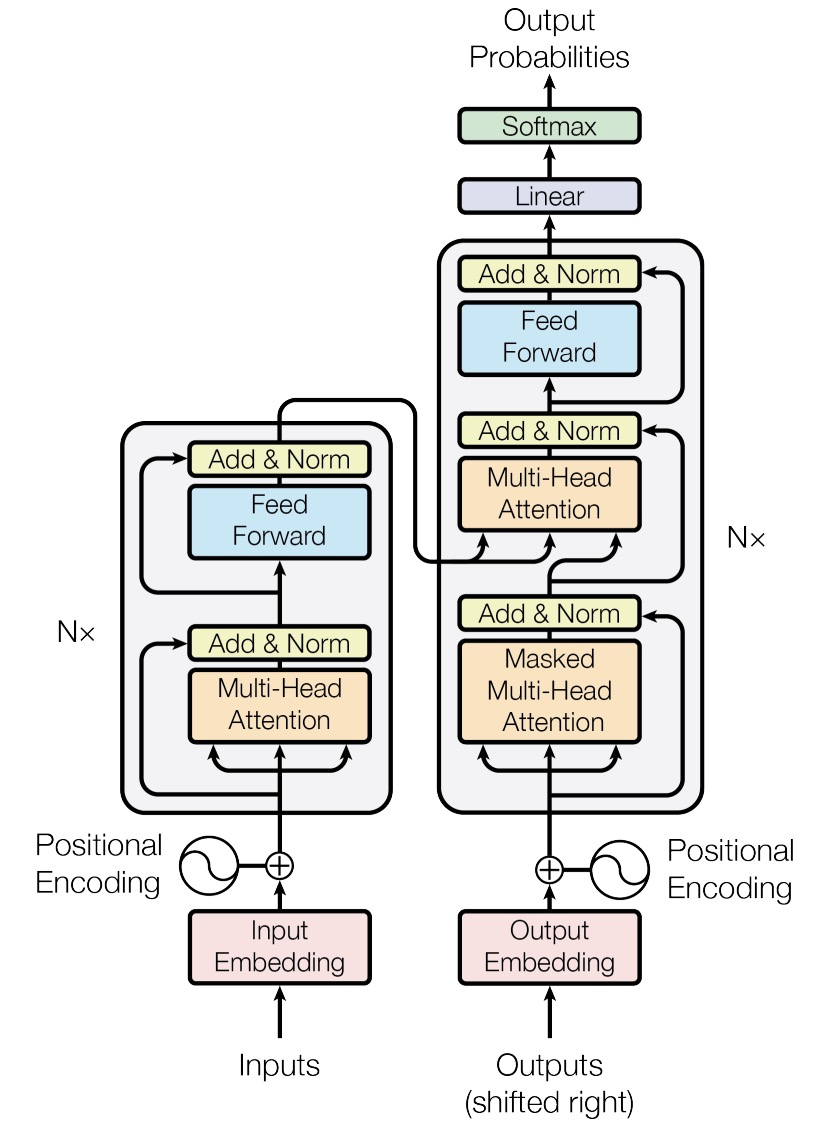
\includegraphics[width=4in]{figures/xulun/transformer.jpg}
  \caption{Transformer 结构框架\cite{vaswani2017attention}}
  \label{fig1:transformer}
  \end{figure}
Transformer 是一个基于注意力机制,特别是自注意力机制的模型,它彻底放弃了循环
神经网络(RNN)和卷积神经网络(CNN)的使用。如\figref{fig1:transformer}, 
Transformer 模型包含两个
主要部分:编码器(左边)和解码器(右边)。每个部分都由多个相同的层
堆叠而成,每层包含了自注意力机制和前馈神经网络,具体描述在\tabref{tab1:encoder}和\tabref{tab1:decoder}中。

\begin{table}[h!]
  \centering
  \small
  \begin{tabular}{lp{10cm}}
  \toprule
  \textbf{子层} & \textbf{描述} \\
  \midrule
  多头自注意力机制 & 允许模型在处理一个单词时,同时考虑句子中的其他单词。 \\
  \midrule
  前馈神经网络 & 它是一个简单的全连接网络,对每个位置的表示应用相同的线性变换。 \\
  \bottomrule
  \end{tabular}
  \caption{编码器结构描述。}
  \label{tab1:encoder}
  \end{table}
  
  \begin{table}[h!]
  \centering
  \small
  \begin{tabular}{lp{10cm}}
  \toprule
  \textbf{子层} & \textbf{描述} \\
  \midrule
  多头自注意力机制 & 与编码器中的自注意力机制类似,但有额外的掩码(Masking)来防止位置获取未来位置的信息。 \\
  \midrule
  编码器-解码器注意力 & 允许解码器关注编码器的输出。 \\
  \midrule
  前馈神经网络 & 结构与编码器的前馈神经网络一致。 \\
  \bottomrule
  \end{tabular}
  \caption{解码器结构描述。}
  \label{tab1:decoder}
  \end{table}

%\textbf{编码器}由相同的层组成。每个层包含两个子层:
%
%多头自注意力机制(Multi-Head Self-Attention):允许模型在处理一个单词时,同时考虑句子中的其他单词。
%
%\textbf{前馈神经网络}(Feed-Forward Neural Network):它是一个简单的全连接网络,对每个位置的表示应用相同的线性变换。
%解码器
%
%\textbf{解码器}同样由多个个相同的层组成,但每个层包含三个子层:
%
%\textbf{多头自注意力机制}(Multi-Head Self-Attention):与编码器中的自注意力机制类似,但有额外的掩码(Masking)来防止位置获取未来位置的信息。
%
%\textbf{编码器-解码器注意力}(Encoder-Decoder Attention):允许解码器关注编码器的输出。
%
%\textbf{前馈神经网络}(Feed-Forward Neural Network):结构跟encoder的前馈神经网络一致。

在Transformer的结构中,注意力机制扮演着核心角色。自注意力机制、缩放点积注意力和多头注意力共同构成了Transformer模型中处理序列数据的基础。

\textbf{自注意力机制(Self-Attention)}
是Transformer结构的基石,它允许模型在处理序列的每个元素时,考虑到序列中的所有其他元素。自注意力的计算公式如下:
\[ \text{Attention}(Q, K, V) = \text{softmax}\left(\frac{QK^T}{\sqrt{d_k}}\right)V \]
其中,\(Q\)、\(K\)、\(V\) 分别表示查询(Query)、键(Key)和值(Value),\(d_k\) 为键的维度。

\textbf{缩放点积注意力(Scaled Dot-Product Attention)}是自注意力机制的一种具体实现,通过缩放因子调整查询和键的点积计算。它提供了一种有效的方法来评估输入元素间的相似度。缩放点积注意力的公式为:
\[ \text{Scaled Dot-Product Attention}(Q, K, V) = \text{softmax}\left(\frac{QK^T}{\sqrt{d_k}}\right)V \]

\textbf{多头注意力(Multi-Head Attention)}
多头注意力机制通过将自注意力分解为多个``头'',在不同的表示子空间中并行执行,从而捕捉输入数据的多样化特征。多头注意力的计算公式为:
\[ \text{MultiHead}(Q, K, V) = \text{Concat}(\text{head}_1, \text{head}_2, \dots, \text{head}_h)W^O \]
其中,每个头 \(\text{head}_i\) 的计算为 \(\text{Attention}(QW_i^Q, KW_i^K, VW_i^V)\),\(W_i^Q\)、\(W_i^K\)、\(W_i^V\) 和 \(W^O\) 是模型中的可学习权重矩阵。

Transformer模型通过其创新的自注意力机制和编码器-解码器架构,为处理复杂的自然语言任务提供了强大的工具。

\subsubsection*{2) Transformer的衍生模型}

随着NLP技术的不断进步,Transformer的衍生模型,如BERT、GPT、XLNet和RoBERTa,
将Transformer结构与无监督学习结合,
可以在不同NLP任务上实现前所未有的性能,无需每个任务重新训练。
这些模型虽采用不同预训练目标和数据集,但依然可根据使用的Transformer结构分类:

\begin{equation*}
  \text{衍生模型} \left\{
      \begin{array}{l}
        \text{Encoder模型(如BERT、RoBERTa),称为自编码模型} \\ 
        \text{Decoder模型(如GPT、XLNet),称为自回归模型。}
      \end{array}
  \right.
\end{equation*}

%\begin{itemize}
%  \item Encoder模型(如BERT、RoBERTa),称为自编码(auto-encoding) Transformer模型
%  \item Decoder模型(如GPT, XLNet),称为自回归(auto-regressive) Transformer模型。
%\end{itemize}


\subsubsection*{Encoder模型}

Encoder 模型只使用 Transformer 模型中的 Encoder 模块,也被称为
自编码(auto-encoding)模型。在每个阶段,注意力层都可以访问到原始输入
句子中的所有词语,即具有``双向''注意力。
Encoder 模型通常通过破坏给定的句子(例如随机遮盖其中的词语),
然后让模型进行重构来进行预训练,最适合处理那些需要理解整个句子语义的任务,
例如句子分类、命名实体识别(词语分类)、抽取式问答。
BERT 是第一个基于 Transformer 结构的纯 Encoder 模型,它在提出
时横扫了整个 NLP 界,在流行的 GLUE 基准上超过了当时所有的最强模型。
随后的一系列工作对 BERT 的预训练目标和架构进行调整以进一步提高性能。
目前,纯 Encoder 模型依然在 NLP 行业中占据主导地位。下面简略介绍一下 
BERT 模型及它的变体RoBERTa。

\subsubsection*{BERT 模型}

BERT是基于 Transformer 架构的自然语言处理模型。它采用 Transformer 的编
码器部分来学习文本中单词或子单词之间的上下文关系。与传统的单向模型不同,
BERT 的编码器一次性读取整个单词序列,因此,虽然通常被描述为``双向''模型,
但更准确地说,它是非定向的。

BERT 的训练涉及两种主要策略:Masked LM (MLM)和Next Sentence Prediction (NSP)。
Masked LM (MLM):在输入序列中随机选择大约15\%的单词并用特殊的[MASK]标记替换,然
后模型尝试预测这些被遮盖的单词。这需要在编码器的输出顶部添加一个分类层,并且通过词嵌入矩
阵将输出向量转换为词汇量,最后使用 softmax 函数计算每个单词的概率。BERT 的损失函数
仅考虑遮盖值的预测。

Next Sentence Prediction (NSP):BERT 接受成对的句子作为输入,并学习预
测第二个句子是否逻辑上紧跟在第一个句子之后。在输入中,50\%是连续的句子对,另一
半则是随机的句子对。在输入模型之前,每个输入序列的开始位置会添加一个特殊的[CLS]标记,
每个句子的末尾添加[SEP]标记,同时引入句子嵌入和位置嵌入。为了预测第二个句子是否跟随
第一个句子,模型将[CLS]标记的输出转换为一个二维向量,并使用 softmax 计算其为连续句子的概率。

BERT 在多个基准测试上取得了显著的成绩,包括 
GLUE、SQuAD、SWAG\cite{zellers2018swag}、CLOTH\cite{xie2018large}、
DREAM\cite{sun2019dream}和 SQuAD 2.0。
BERT 通过这种方式,在理解语言的多个方面,尤其是上下文理解方面,取得了新的突破。然而,由
于其复杂的结构和依赖于大量数据的特点,BERT 在一些情况下难以解释,并且在处理特定类型的
语言数据时可能存在泛化问题。尽管如此,BERT 仍然是自然语言处理领域的一个重要里程碑,并
为后续的模型如 XLNet、RoBERTa 等奠定了基础。

\subsubsection*{RoBERTa 模型}
RoBERTa 模型代表了在深度学习和自然语言处理领域中对
BERT模型的一个重要的进化步骤。这种进化不仅基于对BERT潜力的深入挖掘,而且体
现了对预训练语言模型的深刻理解。在这一过程中,RoBERTa的开发者们采用了四个创
新和优化措施,旨在全面提升模型的性能和适应性。

首先,关于数据集的扩展和训练时长的增加,这些改变源于一个核心理念:更多的数据和
更长的训练周期能够使模型捕捉到更为复杂和微妙的语言模式。通过将数据量从BERT的16GB增
加到160GB,并将训练迭代次数从100K提升至500K,RoBERTa能够在更广泛和多样化的文本上学
习,从而提升其对于复杂语言结构的理解能力。

动态掩码的引入是RoBERTa另一个创新之处。与BERT的静态掩码不同,RoBERTa在每个epoch
中对文本采用不同的掩码模式。这种方法有效防止了模型对固定掩码模式的过度适应,从而推动模型
学习更加泛化的语言表示。具体而言,这种动态掩码策略是在训练过程中实时应用的,确保即使同一
文本在不同的训练阶段也会呈现出不同的掩码模式,增加了训练的多样性和复杂性。

此外,去除BERT中的下一个句子预测(NSP)任务也是一个关键决策。尽管NSP被设计来提高模型
对句子间关系的理解,但研究发现,在去除这一任务后,RoBERTa在多项下游任务中的表现有了显
著提升。这表明对于模型的优化,有时候减法也是一种有效的策略。

再者,RoBERTa在训练中对样本长度的处理也展示了其对复杂语言模式理解的重视。通过在训
练中始终使用全长(512个令牌)的序列,RoBERTa强化了对长距离依赖关系的学习,这对于
处理更为复杂的语言结构至关重要。

这些改进使得 RoBERTa 在多个基准测试(如 GLUE、RACE\cite{lai2017race}、SQuAD 等)
中取得了领先性能,甚
至超过了人类的表现。
综合来看,RoBERTa的这些创新和优化措施共同构成了其卓越性能的基础。通过在大规模数据
集上进行深入训练,实施动态掩码机制,精简训练任务,以及优化样本长度处理,RoBERTa不仅
巩固了BERT作为一种强大的语言模型的地位,也为后续的NLP研究提供了宝贵的参考和启示。


\subsubsection*{Decoder模型}
Decoder 模型只使用 Transformer 模型中的 Decoder 模块。在每个阶段,对
于给定的词语,注意力层只能访问句子中位于它之前的词语,即只能迭代地基于已经生
成的词语来逐个预测后面的词语,因此也被称为自回归(auto-regressive)模型。
下面就简要介绍一些常见的Decoder 模型。

\subsubsection*{GPT 模型}
GPT基于Transformer架构开发,主要使用了该架构的 Decoder 部分。
GPT 结合了 Transformer Decoder 架构和迁移学习方法,
在大量开放在线数据上进行无监督预训练,特别是在 BookCorpus 数据集上。
其预训练任务是根据上文预测下一个单词,从而使模型能够在没有限制的情况下学习语言特征。
此外,GPT 还通过微调适应各种下游任务,如文本蕴含、语义相似性、情感分析等,在包括
SNLI、MNLI、ROC、COPA 和 GLUE 等多个 NLP 基准
测试中取得了显著效果。

然而,GPT 也存在一些局限性,如高计算要求、预训练数据的不完整性及不准确性,
以及在处理高词汇变化的数据方面的泛化问题。

\subsubsection*{XLNet 模型}
XLNet的出现在自然语言处理(NLP)领域引发了显著关注,特别是它在
特定任务中相较于BERT的显著性能提升,标志着NLP模型发展的一个新阶段。这种
模型不仅继承了自回归语言模型的强大特性,同时也融合了自编码语言模型(如BERT)的优
势,创造了一种新的、更为复杂和有效的预训练机制。

XLNet的核心在于它的创新性预训练目标——排列语言模型(Permutation LM)。在
BERT中,模型预训练是通过随机选择一些单词并将其替换为[MASK]标记来进行的,
然后模型被训练来预测这些被掩盖的单词。然而,这种方法导致了一个问题:在实
际应用中,即微调(fine-tuning)阶段,输入数据中并不存在[MASK]标记,这可
能导致预训练和微调之间的不一致性。
为了解决这个问题,XLNet引入了排列语言模型。在这种模型中,对于一个给定长度
的句子,模型会考虑所有可能的单词排列组合。在每次训练迭代中,
模型会随机选择一种排列,并基于这种排列来预测单词。具体来说,对于一个句子中
的每个位置,
模型尝试预测这个位置的单词,给定在这个特定排列中它之前的所有单词。
这种方法有效地模拟了自回归(autoregressive)语言模型的特性,
同时也使模型能够在预训练中学习到上下文的全面信息。

在与BERT的比较中,XLNet的预训练机制展现出三个独特的优势:
首先,BERT通过在输入中随机遮盖某些词并预测这些词来进行训练,而
XLNet则采用了无需明显[MASK]标记的内部随机``遮盖''单词方法。这种差异使得
XLNet在预训练和微调阶段保持了更高的一致性,解决了BERT预训练与微调不一致的问题。

此外,XLNet在处理生成型任务上也表现出明显的优势。得益于其自回归特
性,XLNet能够在维持自然的从左到右的生成过程的同时,内部隐含上下文信
息,这对于生成连贯、流畅的文本尤为重要。

针对长文本的处理能力也是XLNet的一个亮点。它整合了
 Transformer XL\cite{dai2019transformer} 的技术,使
得在处理长文档类型的NLP任务时,相比BERT有着更为显著的优势。

总的来说,XLNet通过结合自回归和自编码语言模型的优势,通过其排列语言模型和注
意力掩码机制,有效地利用上下文信息。这些特性使得XLNet在多项NLP任务中,尤其是在
生成型任务和长文档处理方面,相较于BERT展现出更加卓越的性能。这种创新的预训练方法
不仅解决了先前模型的某些局限性,也为未来NLP模型的发展提供了新的方向。

%\textbf{小结}:
%在本节中,我们对一系列模型进行了深入分析。这些模型主要通过序列化训练数据来学习,
%并在常识性推理任务中表现出色。然而,研究过程揭示了这些模型的一些显著不足。
%首先,即使是经过大规模数据训练的预训练模型,也难以全面掌握全部常识性
%知识\cite{lin2020birds,peng2022copen}。实验结果表明,所有预训练
%语言模型在零样本探测任务上均优于随机猜测,这证明了它们在概念性知识获取方面的潜力。
%然而,即便经过微调,这些模型的准确率仍未能达到人类水平\cite{peng2022copen}。因此,
%探索如何将更多的常识性知识整合到现有模型中,以增强其概念性知识推理能力,成为了一个
%关键的研究方向。

%与此同时,我们也注意到,尽管大型预训练语言模型在NLP领域取得了显著进展并
%在现实世界中得到了广泛应用,
%但它们在处理领域外数据、抵御对抗性攻击\cite{mccoy2019right,jin2020bert}以及应对输入的微
%小扰动\cite{ebrahimi2018hotflip,belinkov2018synthetic}方面仍显脆弱。这些局限性
%可能会阻碍这些模型在实际环境中的安全部署,并影响用户对NLP模型的信任度。为了应对这些
%挑战,语言技术领域的研究者们正加大力度,旨在深入理解并解决这些鲁棒性问题。
%在下一节中,我们将进一步讨论自然语言推理任务中模型鲁棒性的相关研究。

\subsubsection{推理模型鲁棒性研究}
\label{sec1:robustness}
上一小节是我对我所研究的相关的推理方法的介绍,尽管大型预训练语言模型在NLP
领域取得了显著进展并
在现实世界中得到了广泛应用,
但它们在处理领域外数据、抵御对抗性攻击\cite{mccoy2019right,jin2020bert}以及应对输入的微
小扰动\cite{ebrahimi2018hotflip,belinkov2018synthetic}方面仍显脆弱。这些局限性
可能会阻碍这些模型在实际环境中的安全部署,并影响用户对NLP模型的信任度。为了应对这些
挑战,语言技术领域的研究者们正加大力度,旨在深入理解并解决这些鲁棒性问题。
在这一节中,我们将进一步讨论自然语言推理任务中模型鲁棒性的相关研究。
%接下来是对这些模型在具体任务上的鲁棒性的探究的相关工作,
包括模型的鲁棒性的测试和提高模型鲁棒性的相关方法。

\subsubsection*{1. 鲁棒性的定义和测试方法}

Wang等人(2022)\cite{wang2022measure}对模型的鲁棒性进行了定义:

\begin{definition}[鲁棒性]
在自然语言处理(NLP)模型中,\textbf{鲁棒性}指的是模型在面对不同分布的测试数据时保持性能的能力。
具体来说,对于一个输入 $x$ 和它的正确标签 $y$,对于一个在 $(x, y) \sim D$ 上训练的模型 
$f$ 及其对 $x$ 的预测 $f(x)$,鲁棒性是通过模型在测试数据 
$(x', y') \sim D'$(可能与 $D$ 分布不同)上的表现来衡量的。
通常使用诸如鲁棒准确率这样的指标来量化鲁棒性,
定义为 $E_{(x', y') \sim D'}[f(x') = y']$。
\end{definition}

在探讨模型鲁棒性的文献中,可以粗略地将他们分为两类:对抗性攻击下的鲁棒性和分布偏移下的鲁棒性。
对抗性鲁棒性关注在输入 $x$ 周围创建微小扰动 $\delta$ 形成 $x'$ 时模型的表现,
而分布偏移鲁棒性关注在自然发生的不同分布上的模型表现。
这些分类共同探讨 $D'$ 是合成分布偏移(如对抗性攻击)还是自然分布偏移。

\textbf{对抗性攻击下的鲁棒性}:
对抗性鲁棒性的研究主要集中在模型对输入的微小扰动($\delta$)的反应上,
即在原始输入 $x$ 周围引入扰动,形成 $x'$,并观察模型的响应。这类攻击通常通过添加
对人类几乎不可察觉的噪声,以欺骗模型做出错误判断。这种策略最初在计算
机视觉领域被广泛研究\cite{szegedy2014intriguing,goodfellow2014explaining},
随后扩展到自然语言处理(NLP)领域\cite{Marco2020acl,tan2020s,schwinn2023exploring,boucher2022bad},
凸显了对NLP模型进行全面鲁棒性评估的重要性。

\textbf{分布偏移下的鲁棒性}:
与之相对,分布偏移下的鲁棒性关注模型在不同自然分布的数据上的表现。
这类研究反映了现实世界数据多样性和复杂性的影响,如语法错误、方言、
语言差异等因素\cite{blodgett2016demographic, demszky2021learning},以及
同一任务在不同领域的新数据集上的表现。

%对于NLP模型的鲁棒性,已有多项工作尝试理解和测量其在不同任务中的表现
%\cite{tu2020empirical,sagawa2020investigation,geirhos2020shortcut}
%特别是在自然语言推理(Natural Language Inference, NLI)任务中,
%研究者们通过对错误分类样本的分析,确定了导致错误的常见原因,
%并据此构建压力测试集。
CheckList\cite{Marco2020acl}是一个结合了对抗性攻击和分布偏移下鲁棒性测试的方法论。
它借鉴软件工程中的``黑盒测试''方法,重点评估NLP模型在不同输入变化下的表现。这一方法论包括三
个核心部分:功能评估、测试方法和测试用例生成。

1)功能评估:此部分更多关注模型在处理各种NLP任务(如语义角色标注、命名实体识别等)时的能力,
为后续的鲁棒性测试奠定基础。

2)测试方法和测试用例:这里包括对抗性攻击下的鲁棒性和分布偏移下的鲁棒性两个方面。
对于前者,CheckList通过模拟对抗攻击中的微小变化或扰动(如情感分析中的句子轻微修改),
评估模型的反应\cite{goodfellow2014explaining}。它通过不变性测试(INT)和定向期望测试(DIR)等方法,
检验模型在处理对抗性攻击下的鲁棒性(如语法结构变化、情感强度变化)时的稳定性。同时在分布偏移的鲁棒性的测试中,
CheckList通过模板方法简化了大量有效测试用例的创建。
例如,可以创建一个模板``我\{NEGATION\}\{POS\_VERB\}这个\{OBJECT\}'',
并通过不同的词语组合生成多个测试句子,如``我不喜欢这个电影'',来评估模型对否定构造的处理能力。这些例子的主题和分布与原来的测试集已经完全不同。

总结来说,CheckList为NLP领域提供了一个全面的框架,
用于评估和提升模型在面对对抗性攻击和分布偏移时的鲁棒性。
这不仅有助于揭示模型的潜在薄弱环节,也为提高模型的整体鲁棒性提供了实践指导。


%除了CheckList以外,还有很多的压力测试数据集用来测试模型的鲁棒性,下面本文要介绍四个
%常识性推理模型比较常用的压力测试集:

%\textbf{Stress Test数据集}:
%在2018年,Naik及其团队推出了一种创新方法\cite{naik2018stress}来评估自然语言推理(NLI)
%模型的鲁棒性,被称为``Stress Test''。这个方法核心在于探索NLI模型如何应对语言的多样性和复杂性,
%特别是在真实推理能力方面。他们设计了一系列实验,仔细检验了模型在理解\textit{词汇重叠}、\textit{处理否定句}、
%\textit{识别反义词}、\textit{执行数值推理},以及\textit{应对长度不匹配}和\textit{语法错误的句子}等方面的能力。
%此外,这个测试还考察了模型在处理现实世界知识和模糊情境时的表现。
%这种多维度的测试不仅展示了NLI模型在复杂语言处理上的潜力,
%同时也揭示了它们的局限,为未来的研究和改进提供了方向。
%
%\textbf{HANs数据集}:
%在NLI领域的深入研究中,McCoy和同事们在2019年引入了HANs数据集\cite{mccoy2019right},
%致力于解决NLI模型过分依赖简单句法启发式的问题。这个数据集着重检验了模型是否只是依赖于词汇重叠、
%子序列和成分等表面特征来做出判断。研究者们精心设计了一系列模板,每个模板都旨在测试
%特定的启发式策略。这种方法确保了每个测试案例既具有合理性又富有挑战性。HANs数据
%集的发现表明,即使是先进的模型如BERT,在这些句法启发式上也可能表现不佳,揭示了
%这些模型在深层语言理解方面仍有很大的提升空间。
%
%\textbf{Adversarial-NLI(ANLI)数据集}:
%2020年,Nie及其团队引入了Adversarial-NLI(ANLI)数据集\cite{nie2020adversarial},
%标志着NLI领域的一次重大进步。ANLI采用了一种迭代的、对抗性的人机共同循环程序,
%不断地推进数据集的演进并带来新的挑战。在构建这个数据集的过程中,研究团队邀请了非专
%家的人类注释者基于给定的上下文来编写假设,随后使用这些假设的模型预测来引导更多的数据
%收集。这个过程的目的在于发掘并利用模型的弱点。ANLI的创新之处在于其动态和对抗性质,使
%其能够持续适应并挑战最先进的自然语言理解(自然语言推理)模型。这个数据集不仅测试了模型在不同来源
%和上下文中的适应性,而且还推动了自然语言推理领域的界限。
%
%\textbf{Generated FEVER Test数据集}:
%2019年,Schuster及其团队引入了Generated FEVER Test\cite{schuster2019towards},
%这是一个旨在解决事实验证模型中偏见问题的数据集。它检验了在FEVER数据集上训练的
%模型是否仅依赖于索赔中的表面线索而非进行基于证据的深入事实验证。通过创新地构建对称测试集,
%包含原始索赔-证据对及其对立对,Generated FEVER Test迫使模型超越表面线索,
%转向更深入的推理和证据评估。此外,数据集还包含一种重新加权方法,用于调整实例重要性,
%平衡n-gram与标签之间的相关性,特别是针对与特定标签紧密关联的短语。这项工作不仅增加了事
%实验证模型的挑战性,也在创建公平无偏见的数据集方面迈出了重要步伐,显示了模型在处理复杂
%和需要深层理解的情境时的性能下降,从而强调了提升模型在理解和验证事实方面能力的必要性。
%
%这些研究展示了在自然语言处理中,尤其是在自然语言推理任务上,
%针对分布偏移和模型鲁棒性的持续探索的重要性。未来的研究可能会更深
%入地探讨如何系统地识别和应对这些挑战,以及如何整合这些策略以提高NLP系统
%在现实世界应用中的公平性和有效性。
%
\subsubsection*{2. 增强模型鲁棒性的方法}
在自然语言推理领域,增强模型的鲁棒性是一个关键目标。
我们可以将这些增强方法分为两个主要类别:数据增强方法和基于模型和训练方案的方法。

1) 数据增强,作为优化大规模神经网络模型性能的核心策略,
在自然语言处理领域的应用尤为关键。本文概述了几种主要的文本数据增强技术及其在学术研究中的应用,展示了它们如何为自然语言推理任务带来显著的性能提升。

\textbf{回译(Back-translation)}\cite{sennrich2016improving,edunov2018understanding,xie2020unsupervised}:
通过将文本从一种语言翻译到另一种语言,再翻译回原语言,创造出文本的新变体,从而增加数据的多样性。

\textbf{c-BERT词替换}\cite{wu2019conditional}:
运用BERT模型来识别并替换文本中的关键词汇,生成文本的新版本,以此来丰富语料库。

\textbf{混合(Mixup)}\cite{guo2019augmenting,chen2020mixtext}:
通过在不同文本样本之间进行线性组合,创造全新的文本实例。

\textbf{截断(Cutoff)}\cite{shen2020simple}:
分为两类:Token截断,即随机选取Token,将对应Token的嵌入整行置零;特征截断,
即随机选取嵌入的特征,将所选特征维度整列置零。

2) 基于模型和训练方案的方法,一般指的是调整模型结构来增强模型在自然语言推理任务当中的鲁棒性。
最常用的方法是\textbf{对抗性训练}\cite{zhu2019freelb,jiang2020smart},
这种方法通过在词嵌入层引入微小的扰动,合成附加样本,提高模型对异常输入的鲁棒性。
该方法通过梯度反传生成对抗性扰动,并加到原始嵌入矩阵上,产生增强样本,
通常应用于有监督训练场景。

在Qu(2020年)\cite{qu2020coda}的研究中,通过比较这些模型增强技术
在RoBERTa模型上处理自然语言推理任务(MNLI)的效果,发现回译和对抗性训练在提升模型
性能方面效果显著,明显优于c-BERT、混合和截断技术。因此,将回译作为自然语言推理任务中的一
种强有力的基准进行数据增强方法比较,是一种合理的策略。这些研究成果不仅强调了数据增强在提
升模型性能方面的重要性,还为选择适当的数据增强策略提供了宝贵的指导。

\subsubsection{推理模型可解释性研究}
\label{sec1:interpretability}
%上一小节是对模型鲁棒性的一些发现和增强的研究,
%但是我们可以看出即使是覆盖面很广的Checklist也只能说明模型在某些方面,
%比如``semantic role labeling'',``role labeling''或者对抗攻击下的鲁棒性测试,
%但是无法说明到底是什么原因导致的我们可以看出即使是覆盖面很广的Checklist也只能说明模型在某些方面的能力是不足的
%这种解释并不具体,而且里面还涉及人工书写templete,成本较高。

%其他的针对模型不鲁棒的原因的探索还有hypothesis-only 
%和 attention map,hypothesis-only是为了探究分类或者多项选择模型在没有前提只有选项的情况下能否做出正确推理的一种评估模型从
%只看选项这种模式中获益的程度来评估模型是不是没有学习到推理能力,就像我们常说的``三短一长选一长''这种偏差,这种方式从一定程度上说明了问题,
%但是并不完全严谨,因为毕竟模型的真实输入是包含题目的前提的,测试的时候输入的改变可能引起推理方式的改变,
%这种变化不能完全说明原来的推理模式是完全不关注推理能力而是只关注spurious features的。这个方式的另一个弊端就是必须复现模型,如果是模型比较庞大但是资源有限的情况下就很难进行分析。
%
%attention map跟前两种方法相比是一种更直接的white-box的方式,
%大家可以根据attention的权重来分析模型的表现,这看似最科学的方法却已经被证明并不可靠,attention的权重
%并不完全具有可解释性的含义

%所以如何更好的解释模型的表现,比如不鲁棒,就成了一个很重要的课题。

\subsubsection*{1. 模型鲁棒性的限制}
在前一节对模型鲁棒性的深入探讨中,我们注意到这些研究虽然关注了特定任务
(如``语义角色标注''和对抗攻击)下的模型表现,但未能充分解释模型鲁棒性差背后的推理机制\cite{hendrycks2020pretrained}。
例如,Checklist方法\cite{Marco2020acl}
在评估模型某些方面的能力时,未能深入挖掘导致模型不足的根本原因。

\subsubsection*{2. 短路行为的识别及其影响}
这引出了一个关键问题:模型在处理复杂任务时是否真正进行深度推理,
或仅仅是依赖于数据中的简单模式或偏差。这种现象被称为``短路行为''(short-circuit behavior)\cite{huangacombating},
在自然语言推理(NLI)任务中表现尤为明显。McCoy等人(2019)\cite{mccoy2019right}的研究表明,
在NLI任务中,模型可能倾向于依赖关键词或句子结构,而忽略两个句子之间真正的逻辑关系。

\subsubsection*{3. 探索短路行为的方法}

%\Shan{attention map这里有个图, hypothesis only这里加个例子}
为了深入分析和量化机器学习模型中的短路行为,研究人员开发
了``仅假设''测试(``hypothesis-only'')\cite{gururangan2018annotation}和
注意力图(attention map)\cite{vig2019multiscale}这两种方法。这些方法都旨在评
估在缺乏充分上下文信息的情况下,模型是否
过度依赖于选项本身的特征。

1) 仅假设测试

``仅假设''测试的核心思想是检验模型在仅凭假设(即问题或选项本身)的情况下的表现。
这种测试通常用于评估自然语言理解模型。在这种测试中,模型只被提供假设部分,而没
有相应的前提或上下文信息,比如在 \secref{sec1:challenge} 中提到的SNLI的例子,只提供假设
``A man is pushing a baby carriage'' 而不提供前提,让模型猜测前提跟假设之间的关系。
从人的角度来看,
解决这个问题是不可能的,因为问题本身有缺陷,很难做出选择,但是如果模型依然做出跟有前提时一致的结果,
研究者就可以判断模型可能过度依赖于假设中的某些关键词或短语,而忽
略了理解整体意义所必需的上下文。

这种方法的优点在于它能够揭示模型可能的短路行为,即模型可能仅凭借假设
中的关键信息做出判断,而不是进行全面的理解。然而,它的一个限制是无法完全反映
模型在处理真实场景时的推理模式。在现实世界的任务中,模型通常需要综合考虑全面的上下文信息。

2)注意力图

注意力机制是深度学习中的一种重要技术,它帮助模
型聚焦于输入数据的关键部分。注意力图是一种可视化工具,它展示
了模型在做出决策时对不同输入部分的关注程度。通过观察这些图,研究者
和开发者可以更直观地理解模型的决策过程,识别模型关注的是哪些信息。

尽管注意力图提供了一个看似直观的方式来解释模型的行为,但其可靠性
和解释性并非总是确定的。研究表明,即使是通过注意力机制突出显示的部分,也不
一定准确地反映了模型决策的真正依据\cite{jain2019attention}。这意味着,虽然
注意力图为我们提供了洞察模型决策过程的一个窗口,但它并不能完全代表模型的内部工作机制。

总的来说,这两种方法都为理解和评估模型提供了有价值的工具,但它们各有局限性。
理解这些方法的优缺点有助于更全面地评估机器学习模型的行为和决策过程。

%为了更好地理解和量化短路行为,``仅假设''测试(``hypothesis-only'')\cite{gururangan2018annotation}
%和注意力图(attention map)\cite{vig2019multiscale}这两种方法应运而生。
%它们旨在评估模型是否在缺乏完整上下文的情况下,过度依赖于选项本身。
%然而,``仅假设''测试虽然揭示了模型可能的短路行为,但并不能完全反映模型在真实场景下的推理模式。
%同样,尽管注意力图为理解模型的决策过程提供了直观的白盒视角,
%但它的可解释性并非总是可靠\cite{jain2019attention}。

\subsubsection*{4. 数据集偏差对模型性能的影响}
此外,模型的鲁棒性失败有时也可以归因于数据集偏差。
例如,Lewis等人(2021)\cite{lewis2021question}指出,问答模型在训练和测试数据重叠显著的情况下表现更差,
凸显了数据集在模型泛化能力评估中的重要性。在自然语言推理任务中,数据集偏差同样影响
模型性能的准确估计\cite{bras2020adversarial}。

综上所述,为了深入理解和解释模型的推理能力,特别是在面对短路行为时,
我们需要开发更精确的测试方法和分析工具。这不仅将提高模型的透明度和可靠性,
而且将优化它们在复杂真实世界任务中的应用。


%transformer 非常值得参考
%https://transformers.run/back/transformer/
%
%https://zhuanlan.zhihu.com/p/70257427
%
%https://towardsdatascience.com/what-is-xlnet-and-why-it-outperforms-bert-8d8fce710335
%https://www.jianshu.com/p/7677e1a5813c
%
%首先介绍AI 五个范式的变化,然后在五个范式变化中常识性推理相关的研究的相应变化。主要是方法的变化
%https://zhuanlan.zhihu.com/p/615507319
%
%常识性推理的现有研究:综述当前关于常识性推理的研究,包括主要的理论框架、模型和实现方法。
%
%
%可解释AI的相关研究:探讨可解释人工智能的相关工作,特别是那些与常识性推理相关的研究。
%
%
%稳定性在AI系统中的研究:分析稳定性在人工智能系统中的作用,特别是在常识性推理方面的应用。
%
%技术和方法的比较:比较现有技术和方法在处理可解释性和稳定性方面的优势和局限性。
%
%研究差距和挑战:识别当前研究中的空白和挑战,为您的研究定位。
\fi

\subsection{研究内容和贡献}
%我的研究围绕常识性推理领域中的三个重要挑战(\secref{sec1:challenge}中描述)展开:
%第一,提升模型常识性推理能力的挑战;第二,
%解析模型鲁棒性不足的原因的挑战;第三,增强常识性推理模型鲁棒性的挑战。
%针对这些挑战,我们深入分析了现有研究(如\secref{sec1:related}所述),
%特别关注了推理模型和方法(\secref{sec1:approachs})、
%常识性推理模型鲁棒性(\secref{sec1:robustness})
%以及常识性推理模型可解释性(\secref{sec1:interpretability})方面的研究进展。
%下面我将介绍针对这三个挑战我的主要研究内容和贡献。整体结构在\figref{fig1:structure}中表示。
我的研究重点围绕常识性推理领域中的三个关键挑战展开,
如第一节(见 \secref{sec1:challenge})所述。首先是提高模型在常
识性推理方面的能力,其次是解析模型在鲁棒性方面的不足的原因,以及
最后一个挑战,即增强常识性推理模型的鲁棒性。

在下文中,我将介绍我在应对这三大挑战方面的主要研究内容及研究的贡献。
我的研究的整体结构和逻辑框架在图 \figref{fig1:structure} 中有清晰的展示。

\begin{figure}[th]
  \centering\includegraphics[width=5in]{figures/xulun/structure.eps}
  \caption{研究内容的整体结构。}
  \label{fig1:structure}
  \end{figure}


\subsubsection{基于知识增强的常识性推理研究}

\subsubsection*{1. 研究内容}
在应对常识推理任务的首个挑战,即增强模型在常识性推理方面的能力时,
我们的研究聚焦于目前领先的神经网络方法,比如BERT。我们深入分析了这些方法的应用。
虽然神经网络在常识推理任务中展现出强大的性能,
但根据Lin等人的研究\cite{lin2020birds,peng2022copen},在处理常识性知识时,
这些方法仍有提升的空间,特别是在精确把握和表达这些知识时。

为了在常识性推理领域实现进一步的突破,我们选择了一个极具挑战性的任务:
预测叙事故事的结尾。这一任务的设计灵感来源于早期关于故事理解的研究\cite{meehan1977tale},
并随后演化为预测故事中可能发生事件的任务\cite{chambers2008unsupervised}。我们的研究在ROC
故事填空测试数据集\cite{mostafazadeh2016corpus}上进行了实验,
该数据集特别设计用于评估这种预测能力,它要求参与者从两个备选结局中
选择一个最符合四句话故事情境的结局。通过这些实验,我们旨在深入探究并提升模型在
理解和预测故事结尾方面的能力。

相关研究的初步探索集中在如何计算候选结局与故事情境句子之间的语义相似度。
这通常包括对故事句子进行多维度表征,
例如通过句子中词向量的聚合\cite{mikolov2013distributed},应用
sentence2vec\cite{kiros2015skip},DSSM\cite{huang2013learning}或采
用其他创新特征\cite{schwartz2017story}。最新的方法趋向于采用双层结构:
一是利用LSTM\cite{hochreiter1997long},GPT\cite{radford2018improving}或
BERT\cite{devlin2018bert}等预训练语言模型构建句子的深层表征;
二是在ROC数据集上对分类模型进行微调,形成一个全面的故事情境表征。

在此基础上,我们提出了一种新颖的方法,专注于识别和优化故事中的关键概念。
我们发现,在故事推理过程中,将注意力集中在特定关键概念上,而非全部词汇,可以
更有效地指引至正确的结局。因此,我们设计了一种策略,在利用语言模型之前,通过
突出重要概念并降低不重要概念的影响力,来简化句子。这种方法有效地降低了模型处理
的噪音,并使其更专注于捕捉故事的核心信息。这些经过优化的句子被视为事件和概念的集
合,而这些概念在ConceptNet\cite{speer2017conceptnet}——一个全面覆盖常识推理所
需知识的开放领域知识图谱中有所定义。

此外,我们不仅注重于句子内概念的序列化处理,而且还将结构化的常识知识整合进
句子表征中。通过融入预训练的概念嵌入到故事句子表征中,我们能够更准确地捕捉故事情
境与结局之间的关键概念联系。例如,通过\textit{CapableOf}和\textit{MotivatedBy}这样
的预定义关系,我们能够揭示``long for break''与``have a rest''之间的联系,从而在故事中实现更精准的推断。

值得强调的是,我们的方法在ROC故事填空测试数据集上展示了卓越的性能。
尽管现有研究已在故事结局预测任务上取得了一定的进展,但这些成果主要集中
在原始数据集的验证部分。为了确保我们的方法的有效性和泛化能力,我们避免了使
用原始数据集的验证集,而是特意构建了一个新的训练集,该训练集与测试集不共享统
计特征。这种严谨的实验设计使我们的评估结果更加可靠,同时也证明了我们所提出方法
在提高故事理解和预测能力方面的显著效果。

\subsubsection*{2. 主要贡献}

本研究在常识性推理领域引入了一种创新且有效的方法论。我们实施
了一种精心设计的句子简化策略,专注于故事中关键概念的提炼。这种方法不仅
降低了模型处理的复杂性,而且通过集中处理核心信息,极大地提高了模型捕捉
故事情节的精准度。通过将这些精化的概念与ConceptNet数据库中的丰富结构化
知识结合,我们在故事推理任务的准确性上实现了显著的提升。
%这种方法的效果不
%仅体现在故事结局预测的准确率上,更在于其在增强模型处理故事中常识性知识的
%能力方面取得的重大进步。

在实验方法上,我们通过精心筛选和优化的训练数据集来确保了评估的公正性和准
确性。这种方法学的应用不仅提升了故事结局预测的性能,还为常识性推理中结
构化知识的有效运用提供了新的视角。本研究的贡献不仅在于推动了常识性推理领域
的发展,也为未来相关领域的研究提供了宝贵的方法和见解。

\subsubsection{推理模型鲁棒性不足的可解释性分析}
\subsubsection*{1. 研究内容}

从\figref{fig1:structure}中可见,挑战二和挑战三均源于同一现象:推理模型
的鲁棒性不足。尽管多种推理模型在常识性推理任务上取得了显著的成就,但它们在处理
对抗性数据或与训练环境不同的场景时表现出了鲁棒性不足的缺陷。

在探究推理模型鲁棒性不足的原因时,关键在于分析模型处理信息的方法和重点。
研究表明,模型可能过度依赖数据的某些特定结构元素,例如,
在处理\textit{前提}和\textit{假设}的关系时,
它们可能只关注\textit{假设}部分,而忽略了前提与假设之间的逻辑联系\cite{naik2018stress,mccoy2019right,schuster2019towards,nie2020adversarial}。
这揭示出模型可能主要学习数据中的统计偏差,也就是所谓的偏见线索(bias cues)或者
虚假线索(spurious cues)。

对这一现象出现的原因一种假设是数据集的构建方式存在偏见。模型往往学习特定于
数据集的简化规则或者偏见,而非解决问题的通用策略。例如,在自然语言处理中,如
果一个数据集中的大多数``正确''样本都包含某个特定词汇,模型可能仅依赖这个词
汇做出判断,而未深入理解句子间的逻辑关系。这种简化学习方式导致模型在面对
结构或上下文有差异的新数据时变得脆弱,无法有效适应或正确解释。如果这种线索刚好在\textit{假设}部分,
那可能就会造成模型只关注\textit{假设}部分。

为验证模型可能过度关注数据特定结构元素的假设,研究者们开发了``仅假设''测试\cite{gururangan2018annotation}和
注意力图\cite{vig2019multiscale}
这两种方法来分析和量化这一现象。尽管这些工具在解析和评估模型行为方面
发挥着关键作用,它们在深入探讨数据偏见如何影响模型核心机制方面存在局限性。
因此,深入研究数据偏见对模型机制的具体影响已成为一个紧迫且重要的研究课题。

对此问题,我们设计了两种测试框架来应对这一挑战。第一种是宏观层面的测试框架,基于统计特
征来进行评估;第二种则是微观层面的详细统计分析框架。

%从\figref{fig1:structure}中我们可以看出挑战二和挑战三都来源一个现象,
%就是推理模型的鲁棒性差这个现象
%虽然很多推理模型在众多常识性推理任务上取得了显著成就,
%但是它们在处理对抗性数据或不同于训练环境的场景时仍显脆弱。
%这种局限性通常源于模型对数据集中特定模式的过度依赖,而非深入理解问题本
%质\cite{naik2018stress,mccoy2019right,schuster2019towards,nie2020adversarial}。

%虽然已有一些研究努力揭示了模型学习过程中的
%一些不足,如CheckList\cite{},但对于模型学习到的具体内容还需更加精细和系统的分析。
%因此,我们提出了两种测试框架:一种是宏观层面上基于统计特征的测试框架,
%另一种则是微观层面的详细统计分析框架。

%在解决第三个挑战时,即深入探讨常识性推理模型鲁棒性不足的根本原因,
%正如\ref{sec1:interpretability}小节所述,
%我们发现模型鲁棒性的评估过程不仅揭示了模型的潜在不足,如通过工具Checklist等所指出的,
%而且还暴露了模型可能倾向于学习短路(short-circuits)或虚假特征(spurious features)。
%然而,这些评估方法虽然提供了宝贵的见解,但在深入探究模型确切学到了什么方面,
%尚存在一定的探索空间。这意味着,虽然已有一些研究努力揭示了模型学习过程中的
%一些特征,但对于模型学习到的具体内容和其背后的复杂动态,还需更加精细和系统的分析。
%因此,我们提出了两种测试框架:一种是宏观层面上基于统计特征的测试框架,
%另一种则是微观层面的详细统计分析框架。

\subsubsection*{宏观层面的统计特征测试框架}

在宏观层面,我们的研究主要集中于分析自然语言推理任务中的虚假线索问题。
我们注意到,尽管人类在处理这类问题时通常会分析问题前提与假设之间的逻辑关系,
许多NLP模型却倾向于主要关注假设部分,忽略了深入的逻辑分析。这种现象往往是由
于数据集中的人为偏差所引起。

在评测和分析数据集方面,我们提出了一种基于统计学线索发现的方法。
这个方法首先应用统计学公式来拟合``仅假设''模型,以便识别数据集中最具代表
性的统计特征。这种方法不仅揭示了数据集中的偏见和虚假线索,还为我们提供了一
种衡量数据集质量的有效工具。

进一步地,我们设计了一种多次采样测试方法,将测试数据划分为简单和困
难两类。这种划分旨在衡量模型在处理复杂推理任务时的真实能力,同时量
化比较简单和困难子集之间的性能差异。通过这种方法,我们能够评估模型是
否过度依赖于数据中的简单线索,从而揭示模型在不同情境下的潜在弱点。

此外,这种宏观评估方法不仅揭示了数据集的质量,还为我们提供了关于模型在
逻辑推理能力上的深刻见解。这种方法的应用有助于我们理解模型在解决自然语言推理任务时的
潜在限制,并指导我们如何改进模型以提高其泛化能力和鲁棒性。

\subsubsection*{微观层面的统计分析框架}
在更细致的层面,我们采用了微观统计分析框架--ICQ(``I-see-cue'',即``我发现线索'')框架,
这一工具旨在揭示和分析自然语言推理任务中数据集和模型的偏见性线索。ICQ框架的
应用分为两个主要领域:一是探索数据集中潜藏的偏见线索;二是评估偏见线索对模型性能的影响。

在数据集分析方面,ICQ框架旨在识别可能在数据集制作过程中不经意间引入的偏见性线索。
这些线索可能表现为特定词汇的使用、独特的短语结构或特别的语境模式。通过分析
这些线索的词汇频率、共现模式以及它们与目标标签的关联性,ICQ揭示了潜在的误
导源,增强了我们对数据集如何影响模型预测的理解。

在模型分析方面,ICQ重点分析自然语言推理模型如何在训练过程中学习和依赖这些线
索。我们采用了准确性测试和分布测试两种方法,以全面了解模型对数据集中
的偏见性线索的敏感度。准确性测试揭示了模型在处理包含或缺失特定线索的数
据样本时的表现,从而展示了模型对这些偏见性线索的依赖程度。而分布测试则
通过可视化分析,探究了特定特征分布的变化如何影响模型的预测性能,为我们提供了更直观的理解。

将这两种测试方法结合,ICQ框架为我们提供了一个全面的视角,以分析和评估
模型在学习和反应偏见性线索方面的行为。这种综合性的分析方法不仅增强了我们
对模型行为的认识,还促使我们在发现偏见时采取相应措施,以提高模型在处理具有潜
在偏见的复杂数据时的鲁棒性和推理能力。这对于构建更加公正、高效的自然语言推理系统具有重要意义。

%在更细致的层面,我们采用了微观统计分析框架,该框架结合模型的表现对测试集进行多维特征划分。
%通过这种方法,我们能够对模型在各个特征上的准确性测试和分布测试的表现进行深入分析,
%进而解释模型是否对某些分布不均衡的特征过于敏感。此外,我们还开发了一种可视化工具,
%以直观地展示这些测试结果,帮助研究人员更有效地识别和理解模型性能差异的潜在原因。

%\subsubsection*{方法和应用}

%通过深入分析神经网络模型在自然语言推理、论证分析和常识推理等任务中的表现,
%我们注意到这些模型可能倾向于利用数据集中的表面统计模式来预测正确答案。例如,
%在SNLI数据集中的多项选择问题中,模型可能仅依赖假设就能找到正确答案,这揭示了数据
%集中手工制作假设的人为误差。
%
%为应对这些问题,我们提出了ICQ(``I-see-cue'',即``我看到线索'')框架,这
%是一个灵活的统计分析工具,用于识别多项选择自然语言推理数据集中的简单但有影响力的
%线索。与传统方法相比,ICQ无需额外的测试案例即可识别自然语言推理数据集中的偏见。它采用黑
%盒测试方法,不仅评估模型如何利用这些偏见,而且为理解自然语言推理任务中的偏见提供了全面的视角。
%
%我们在各种自然语言推理数据集上部署ICQ,探测了模型在训练期间可能学到的线索。ICQ有
%助于深入理解模型如何学习潜在偏见,并为其实际应用提供了宝贵的见解。

\subsubsection*{2. 主要贡献}

本研究的主要贡献在于开发了这两种创新的分析框架,
它们为深入理解并提升常识性推理模型的鲁棒性提供了新的视角。
通过宏观和微观的方法,我们能够全面评估模型在面对复杂数据时的行为,
特别是在识别和处理潜在的虚假特征方面。这不仅有助于揭示模型可能的薄弱环节,
也促进了对模型学习机制的深入理解,为未来设计更为健壮和可解释的人工智能系统奠定了基础。

本研究的主要贡献在于开发了这两种创新的分析框架,
它们为深入理解常识性推理模型的鲁棒性不足的现象提供了新的视角。
%本研究的主要贡献在于深度探究和分析自然语言理解(自然语言推理)任务中的数据集和模型之间的复杂相互作用,特别是通过宏观和微观角度的综合分析,揭示了数据集中的偏见性线索及其对模型行为的影响。

在宏观层面,我们分析了自然语言推理数据集的结构和内容,探究了如何在数据
集创建过程中可能不经意间引入的偏见性线索。通过识别这些数据集中的特
定词汇使用、独特的短语结构,我们深入理解了这些偏见是如何形成的,以及它们可
能如何导向模型的预测。

微观层面的分析则集中在应用ICQ框架,一个专为分析模型对数据集中偏见性线索
的响应而设计的工具。通过ICQ,我们进行了准确性测试和分布测试,深入探讨了模型
如何在训练过程中对这些线索产生依赖,以及这种依赖如何影响模型的推理能力和整体性
能。ICQ的应用使我们能够更细致地观察模型对特定特征分布变化的敏感性,为理解模型行为提
供了更加丰富和直观的视角。

这两个层面的分析相辅相成,它们共同揭示了自然语言推理任务中数据集与模型之间的复杂关系,尤其
是在理解和处理偏见性问题时。本研究不仅为理解自然语言推理系统中的数据集和模型交互提供了深
入的见解,也为构建更加公平、有效且鲁棒的自然语言推理系统提供了实践上的指导。这些贡献对于未
来在该领域的研究和应用具有重要的意义,为改进数据集质量和提升模型处理能力提供了支持。

\subsubsection{提升常识性推理模型鲁棒性的数据增强策略}

\subsubsection*{1. 研究内容}
%在应对常识性推理模型鲁棒性不足的挑战时,
%我们在\secref{sec1:robustness}中探讨了模型鲁棒性的定义和测试方法。
%研究指出,尽管神经网络模型在多个任务上表现出色,其鲁棒性的不足却严重限制了模型的泛化能力。
%并且在上一节对模型鲁棒性不足的解释中,我们也发现了数据偏差对模型的巨大影响。
%为此,我们提出了创新的数据增强方法,旨在提高模型的泛化能力并减少数据统计偏差。
本研究着眼于提升常识性推理模型在自然语言推理任务中的鲁棒性的挑战,
尤其是在处理多项选择题(MCQs)时面临的挑战。多项选择题是评价常识性推理任务的常用格式,
涵盖因果推理~\cite{roemmele2011choice}、故事结尾预
测~\cite{mostafazadeh2016corpus,huang20story}、论
证理解~\cite{habernal2018argument}以及阅读理解~\cite{yu2020reclor}等任务
等多个领域。虽然这些格式在理论上被认为
是有效的评估工具,但最新的研究发现,许多先进的神经网络模型在处理这类问题时,并
没有真正理解问题的逻辑和语义,而是依靠数据中的统计特征或偏见进行判断。这一发
现揭示了一个重要的问题:在自然语言推理任务中,这些模型展现出了一种我们称之为``短路行为''的现象。

这种``短路行为''指的是在MCQs问题中,模型在没有充分理解问题内容的情况下,依靠数据
中的表面规律或偏见来作出判断。这一行为不仅限制了模型的泛化能力,也挑战了我们评
估其真实理解能力的方法。因此,在本研究中,我们将探索和开发新的方法和技术,旨在更
精确地识别和克服这种行为,从而提高模型在各类自然语言推理任务中的鲁棒性和有效性。

为了深入探究和量化这种``短路行为'',我们超越了传统的``仅选项测试''方法。我们发
展了一种新颖的``代理测试''方法,这种方法不仅从宏观层面评估模型的行为,而且通过构建
专门针对``短路行为''设计的新题目,远离了传统的``仅假设''框架。这种代理测试方法能够
更精准地揭示模型在面对复杂任务时的真实处理机制。

为了进一步增强数据处理能力,我们采用了``交叉''和``变异''两种数据增强策略。
这些策略旨在创造具有挑战性的新训练实例,推动模型超越对数据中表面统计规律的依赖,
深入理解问题的本质。

``交叉''操作灵感来自生物遗传中的染色体交叉过程。具体操作是,我们将两个不同问题的选项进行互换,
以创造全新的问题实例。例如,从两个不同的MCQs中各取一个选项,交换它们的位置,从而生成具有新
组合的问题。这种方法在模型的训练中引入了额外的复杂性和多样性,迫使模型去更深层次地理解问题
和选项之间的关系。

而``变异''操作则是对原始问题的某些元素进行细微的调整或修改,以增加问题的复杂性和多样性。这类
似于在生物进化中的基因突变,通过对问题或选项中的关键词或短语进行轻微的变化,产生新的问题版
本。这些创新性操作
能够产生全新的、具有挑战性的训练实例,促使模型超越表面的统计规律,
深入学习问题的内在逻辑和结构。

将这些策略应用于当前领先的神经网络模型,如BERT\cite{devlin2018bert}、XLNet\cite{yang2019xlnet}
和RoBERTa\cite{liu2019roberta},并在COPA\cite{roemmele2011choice}、ROC\cite{mostafazadeh2016corpus}、ARCT\cite{habernal2018argument}和
RECLOR\cite{yu2020reclor}等多个基准数据集上进行测试。我们的实验结果显示,这些数据增强策略显著提高了模型在对
抗性数据环境中的准确性,并在原始测试集上也实现了性能的提升。


\subsubsection*{2. 主要贡献}
在本研究中,我们主要贡献在于开发了两种高级的数据增强方法,
旨在提高常识性推理模型在多样化数据环境下的鲁棒性。
灵感来源于生物学的``交叉''和``变异''的数据生成方法的应用
经过了在多个基准数据集上的全面测试,证明了它们不仅能够提升模型在``短路问题''代理测试中
的表现,而且也能在标准评估环境下维持或提高性能。通过这些创新,我们的研究不只是强化了模型对多
样化和对抗性数据的处理能力,也为提升AI系统在真实世界应用中的泛化能力和可靠性提供了新的视角
和工具。

%本研究的主要贡献在于系统性地提高了常识性推理模型在多项选择
%题(MCQs)中的鲁棒性,尤其突出在自然语言理解任务的复杂环境中。核心成
%果涵盖了对现有自然语言推理模型中普遍存在的``短路行为''的深入识别与评估,以及针对该
%问题的创新性解决方案的开发和实施。
主要贡献可以细分为下面三点:

\textbf{1) 深入揭示和评估``短路行为''}: 我们首次系统性地揭示了模型处理MCQs任务时的一种关
键弱点——``短路行为'',即模型依赖于数据中的偏见或统计特征而非深入理解上下文和逻辑关
系。通过开发``代理测试'',我们不仅扩展了传统的测试范围,而且专门针对这种行为进行了精准的评估。

\textbf{2) 开发创新的数据增强策略}:``交叉''和``变异'': 我们提出并实施了两种创新的数据增强策略,即``交叉''和``变异''。这些策略有效地引入了更高的问题复杂性和多样性,迫使模型超越对表面统计规律的依赖,深入理解问题的本质。这一策略在提高模型对复杂任务的理解和处理能力方面展现了显著效果。

\textbf{3) 显著提升模型鲁棒性和性能}: 应用这些策略于领先的神经网络模型并在多个基准
数据集上进行测试后,我们的实验结果证实了这些方法不仅在压力测试中显著提升了模型的准确性,
而且在常规测试环境中也增强了模型的整体性能。这一成果标志着我们的方法不仅成功地解决了``短路行为''
的问题,而且在提高模型在多样化和对抗性数据环境下的整体鲁棒性方面取得了重要进展。

总体而言,本研究为自然语言推理领域提供了关于模型行为深度理解的新视角,并为提升模型在复
杂数据环境中的泛化能力和可靠性提供了创新且有效的工具和方法,对构建更加鲁棒和可靠
的自然语言推理系统具有重要的实际意义。


\subsection{章节安排}

在本研究的绪论中,我们对常识性推理的研究背景进行了深入剖析,全面探讨了
人工智能和自然语言处理领域的发展历程,以及在常识性推理领域所面临的挑战。针对
这些挑战,我们提供了一个概括性的概述,介绍了为应对每项挑战而开展的研究内容及其主
要贡献,特别强调了在提升常识性推理能力、增强模型鲁棒性和深化模型可解释性方面
所取得的进展。接下来的第三至五章将对每项研究进行更加具体的介绍。

第二章中,我们对与常识性推理紧密相关的关键研究领域进行了详细的梳理,包括任
务的界定、基准数据集的构建、推理模型的方法论,以及这些模型在鲁棒性和可解释性
方面的最新研究进展。我们对数据集和推理模型的方法论进行了系统性的介绍,这些内
容将在后续章节中被频繁引用。

在第三章中,我们着重探讨了如何有效提升模型在常识性推理方面的能力,这是应对
常识性推理领域的首个核心挑战。本章详细介绍了我们提出的一种新颖方法论,这包
括故事中关键概念的识别与处理,以及通过精简关键概念来减轻模型对次要概念的依赖。此
外,本章还探讨了如何通过融合结构化常识知识来深化对故事情境的理解。我们在ROC数据集
上进行的实验展示了通过概念简化和知识图谱融合技术,我们的方法如何显著提升故事结局预测的准确性。

第四章深入探讨了解析常识性推理模型鲁棒性不足的原因,并提出了两种用于深化理解模型性
能的分析框架。我们首先开发了一个宏观层面的统计特征测试框架,用以评估模型在识别和
学习虚假特征的能力。随后,我们引入了微观层面的详细统计分析框架(ICQ),对模型在不同特
征上的表现进行了深入的分析。这些框架展示了如何为设计更健壮和可解释的AI系统提供新的方法和视角。

第五章则聚焦于提高常识性推理模型鲁棒性的关键策略,特别是在面对多样化和对抗性数据环境
时的性能提升。本章介绍了两种创新的数据增强方法:通过在训练数据中注入噪声以减少统计偏
差,以及灵感来源于生物学中的``交叉''和``变异''机制的方法,以创造新的训练实例。这些方法在
多个基准数据集上的测试结果表明,它们能够显著提升模型的鲁棒性,减少``短路''问题,同时在标
准测试集上保持或提升性能。

第六章主要对本论文的工作进行总结,并展望未来可能的研究方向。在这一章节中,我们将回顾
研究的主要成果,并讨论未来研究可能探索的新领域。

\newpage
\null
\newpage

\newpage
\fancyhead[LH]{上海交通大学学位论文}
\fancyhead[RH]{第二章\quad 研究现状}
\setcounter{figure}{0}
\setcounter{table}{0}
\section{研究现状}
\label{sec1:related}
在上一节的内容中,我们回顾了过去十年间人工智能(AI)和自然语言处理(NLP)领
域所取得的显著进展,并探讨了常识性知识领域的进步如何为常识性推理研究提供重要支撑。
此外,我们还分析了在这常识性推理领域所面临的挑战,概述了我们在应对这些挑战时主要的研究内容和贡献。
为本章内容的深入探讨奠定了基础。本章旨在全面介绍常识性推理的研究现状,
涵盖从主要任务和评估基准到近年来流行的方法和模型,以及这些模型在可
解释性和鲁棒性评估方面的研究进展。

本章首先聚焦于常识性推理领域的核心任务及其相关评估基准(benchmarks),以
此为出发点,探讨了任务的具体内容、目标和挑战。随后,我们将深入讨论推理模型
的方法论,包括符号方法、早期统计方法以及神经网络方法,并详细分析这些方法的
优势和局限性。这些数据集和推理方法将在后续章节中将被频繁引用。

接下来,本章将重点探讨推理模型鲁棒性的研究。这部分内容包括鲁棒性的定义、测
试方法,以及用于增强模型鲁棒性的各种策略。我们将深入分析模型所面对的多样化和对
抗性数据类型,并探索提升这些模型鲁棒性的有效途径。

最后,本章将探讨推理模型的可解释性研究,包括模型鲁棒性不足现象分析、模型鲁棒性不足的
原因的假设和验证方法。
这一部分的内容对于理解模型在复杂环境下的行为模式及其背后的原因至关重要。

综上所述,本章将为读者提供一个全面而深入的视角,以理解常识性推理领域的当
前研究现状,包括其核心任务、评估基准、方法论以及鲁棒性和可解释性的研究进展。



%在上一节中,我们细致回顾了过去十年间人工智能(AI)和自然语言处理(NLP)领域所取得的重大进步。我们不仅探讨了这些进步对于常识性推理研究的重要性,
%还分析了在这一研究领域中所面临的挑战。本章将深入介绍常识性推理的研究现状。
%我们首先将探讨此领域所涵盖的主要任务及其相关的评估基准(benchmarks),随后,
%会详细讲述近年来流行的方法和模型,以及这些模型在鲁棒性方面的评估方法(包括解释性评估)和提升策略。

\subsection{任务}
\label{sec1:task}


在常识性推理领域,存在多个关键任务\cite{storks2019recent},每个任务都在理解和推动人工智能发展中发挥着至关重要的作用。以下为这些任务的详细介绍:
\begin{enumerate}
  \item \textbf{Reference Resolution(指代消解)}:
  指代消解任务涉及识别文本中特定表达式(如代词或短语)所指代的对象。这一任务对于自然语言处理至关重要,它不仅要求理解语言的上下文,还要求捕捉到语言的隐含意义。复杂句子中的多个名词和代词之间的准确指代关系识别,
  不仅需要深入理解句中实体间的关系和上下文环境,有时更需借助外部常识性知识\cite{morgenstern2016planning,davis2017first}。
  指代消解是理解复杂文本和对话的基础,对于提升机器的语言理解能力至关重要。

  \item \textbf{Question Answering(问题回答)}:
  这个任务要求对特定文本片段进行深入理解,以回答有关该文本的问题。这不仅考验了机器在处理语法和词汇基础上的能力,
  也考验了其在理解文本、提取关键信息、逻辑推理乃至应用外部知识等方面的能力。机器必须能够理解文本的深层含义,
  并在必要时利用广泛的背景知识来进行回答。

  \item \textbf{Textual Entailment(文本蕴涵)}:
  文本蕴涵是由Dagan等人(2005)\cite{dagan2005pascal}定义的,指的是文本与假设之间的方向性关系,其中如果一个典型人根据文本会推断假设为真,
  则可以说文本蕴含假设。一些基准测试通过要求识别矛盾来扩展这项任务,例如第四和第五届RTE挑战\cite{giampiccolo2008fourth,bentivogli2009fifth}。
  与问题回答相似,文本蕴涵任务需要利用多种简单的语言处理技能,例如命名实体识别和共指解析。
  不同于问题回答,文本蕴涵还需要理解一个典型人可能做出的推断,因此常识性知识对于这个任务至关重要。

  \item \textbf{Plausible Inference(合理推理)}:
  Davis和Marcus(2015)\cite{davis2015commonsense}定义的合理推理任务要求系统在有限上下文中做出合逻辑的、中间性的或不确定性的结论。
  这涉及到在故事中断的关键时刻,选择或生成最合理的后续事件。系统不仅需理解给定信息,
  还需运用常识性知识和逻辑推理预测最可能的结果。

  \item \textbf{Intuitive Psychology(直觉心理学)}:
  %\Shan{注意这里ROC举的例子}
  直觉心理学是合理推理任务中的一个重要领域,涉及通过行为推断情感和意图,这是人类的一项基本能力。
  有些基准测试在某些示例中涉及这个主题。%例如ROC\cite{mostafazadeh2016corpus}在表\ref{tab:table1}中的求婚例子,
  直觉心理学任务集中于理解和推断人类行为背后的动机、情感和意图。系统需要理解文本中的事实信息,并对人物的心理状态和社会互动进行深刻洞察。

  \item \textbf{Multiple Tasks(多任务)}:
  一些基准测试由几个单独的语言处理或推理子任务组成,以便在统一的格式下学习和测试不同的阅读理解技能,
  比如bAbI\cite{weston2016towards}和GLUE\cite{wang2018glue}。这些基准可以用作诊断工具,
  以确定模型在不同领域的表现。子任务通常是从各种已存在的基准测试中重新框定的\cite{white2017inference}。
  这些基准对于全面评估和提高人工智能系统的语言处理能力至关重要。
\end{enumerate}

\subsection{基准数据集}
\label{sec1:benchmarks}
%\Shan{注意之后所有arct\_adv改成STS}
%在探索常识性推理领域时,本文重点关注了\secref{sec1:task}所提及的若干关键任务。
%这些任务对于理解和推进人工智能的发展起着至关重要的作用。特别地,本节深入探讨了与这
%些任务紧密相关的主要数据集。这些数据集不仅为研究者提供了丰富的实验资源和标准化评估基准,
%而且直接映射出当前自然语言处理技术的成就与挑战。下面的表格(\tabref{tab1:datasets})列出
%了与各种任务类型相关的关键数据集。

在探索常识性推理领域时,我们特别关注了\secref{sec1:task}中提及的若干关键任务,
每个任务都在理解和推动人工智能发展方面扮演了至关重要的角色。本小节重点介绍了
与这些任务紧密相关的主要数据集。这些数据集不仅为研究提供了丰富的实验材料和
标准化的评估基准,还直接反映了当前自然语言处理技术的发展水平及其面临的挑战。
下面的表格(\tabref{tab1:datasets})详细展示了各种任务类型相关的关键数
据集,包括SNLI\cite{bowman2015large}、MNLI\cite{williams2018broad}、
QNLI\cite{wang2018glue}、COPA\cite{roemmele2011choice}、
ROC\cite{mostafazadeh2016corpus}、SWAG\cite{zellers2018swag}、
RACE\cite{lai2017race}、RECLOR\cite{yu2020reclor}、
FEVER\cite{thorne2018fever}、
STS\cite{schuster2019towards}、
ARCT\cite{habernal2018argument}、
CQA(CommonsenseQA)\cite{talmor2019commonsenseqa}和
Ubuntu\cite{lowe2015ubuntu}。


接下来,我们将对\tabref{tab1:datasets}中提到的每个数据集的格式以及其主要特点进行详细介绍,
以更深入地理解它们在评估不同推理任务中的作用和重要性。

\begin{table}[th!]
  \centering
  \scriptsize
  \begin{tabular}{
  >{\centering\arraybackslash}p{0.15\textwidth}|
  >{\centering\arraybackslash}p{0.20\textwidth}|
  >{\centering\arraybackslash}p{0.10\textwidth}|
  p{0.28\textwidth}}
      \toprule
      \textbf{数据集} & \textbf{任务类型} & \textbf{任务格式} & \textbf{特点} \\ 
      \midrule
      SNLI & 文本蕴涵 & 分类 & 成对句子判断蕴涵关系 \\ 
      \midrule
      MNLI & 文本蕴涵 & 分类 & 多体裁文本蕴涵 \\ 
      \midrule
      QNLI & 文本蕴含,问题回答 & 分类 & 问题与回答的判断 \\ 
      \midrule
      ROC & 合情推理 & 多项选择 & 选择故事合理结尾 \\ 
      \midrule
      COPA & 合理推理 & 多项选择 & 因果或效果的选择 \\ 
      \midrule
      SWAG & 合情推理 & 多项选择 & 预测情境后续 \\ 
      \midrule
      RACE & 合情推理 & 多项选择 & 中高中水平阅读理解 \\ 
      \midrule
      RECLOR & 合情推理 & 多项选择 & 逻辑推理阅读理解 \\ 
      \midrule
      FEVER & 合理推理 & 分类 &用于评估模型在事实验证方面的能力 \\ 
      \midrule
      STS & 合情推理 & 分类 &  测试声明和相应证据的准确性\\ 
      \midrule
      ARCT & 问题问答 & 分类 & 论证有效性评估 \\ 
      \midrule
      CQA & 问题问答 & 多项选择 & 评估常识性知识理解 \\ 
      \midrule
      Ubuntu & 问题问答 & 多项选择 & 对对话模型的评估 \\
      \bottomrule
  \end{tabular}
  \caption{常识性推理数据集概览。}
  \label{tab1:datasets}
\end{table}




%接下来,我们将对\tabref{tab1:datasets}中提到的每个数据集进行更深入的介绍,以便更好地理解它们在各自任务中的应用和重要性
1. SNLI(Stanford Natural Language Inference):
如\tabref{tab1:datasets}所示,Stanford Natural Language Inference(SNLI),
由Bowman等人于2015年提出(参见文献\cite{bowman2015large}),是一项基准测试。它包含近60
万个句子对,旨在执行类似于第四和第五届RTE挑战(参见文献\cite{giampiccolo2008fourth,bentivogli2009fifth})
的三种推理任务。除了标准的蕴涵、矛盾和中立标签,SNLI数据集还特别包含了五种群体判断标签,
这些标签反映了对每个判断的信心程度和一致性水平。

2. MNLI(Multi-Genre Natural Language Inference): 
由Williams等人提出\cite{williams2018broad},包含433,000个示例,是目前最大的自然语言推理语料库之一。
它涵盖了十种不同体裁的书面和口语英语,旨在涵盖现代标准美国英语使用的全部多样性。
所有体裁都出现在测试和开发集中,但只有五种体裁包含在训练集中。
这种设计允许研究者评估模型在已知来源(匹配)和未知来源(不匹配)的测试示例上的表现。
MNLI数据集的目的是推动自然语言理解(NLU)领域的研究,特别是在领域适应和跨领域转移学习方面。

3. QNLI(Question Natural Language Inference)数据集\cite{wang2018glue}: 
是基于SQuAD(Stanford Question Answering Dataset)\cite{rajpurkar2016squad}构造的,
SQuAD由Rajpurkar等人(2016)提出,
专注于自然语言理解和问题回答任务。
SQuAD包含超过10万个问题,旨在从Wikipedia文章段落中找到问题的答案。
QNLI从SQuAD中提取段落和问题,转换成自然语言推理的形式,
即给定一个声明(问题)和一个文本片段(段落),要求模型确定文本是否包含该声明的答案。
这种转换允许QNLI评估模型在理解复杂文本及其隐含含义的能力,尤其是在深入分析和推理的背景下。

4. COPA(Choice of Plausible Alternatives)\cite{roemmele2011choice}: 由Roemmele等人在2011年提出,是一个专注于评估事件之间因果推理的任务。
这个任务需要常识知识来判断通常在世界上发生的事件。COPA提供一个前提和两个选择,
要求从中选择一个作为最合理的原因或效果,测试模型的向前或向后因果推理能力。
数据集包含1,000个这样的实例,是评估模型在理解和推理因果关系方面的能力的重要工具。

5. ROC\cite{mostafazadeh2016corpus}: 由Mostafazadeh等人在2016年提出,是一个专注于日常生活故事的语料库,包
含大约50,000个五句话故事。这些故事涵盖了丰富的因果和时间关系,
非常适合于学习和评估常识性知识。其中大约3,700个故事被指定为测试用例,
每个测试案例包含一个合理和一个不合理的备选故事结尾,供模型在故事闭幕测试中进行选择。
这个测试是Chambers和Jurafsky(2008)提出的
叙事任务\cite{chambers2008unsupervised}的一个更具挑战性的替代方案,
旨在评估模型理解故事情节和进行逻辑推理的能力。

6. SWAG(Situations With Adversarial Generations)\cite{zellers2018swag}: 由Zellers等人(2018)提出,
是一个包含大约113,000个文本开头的基准数据集,每个文本开头有四个可能的结尾。
这个基准测试旨在评估模型在情境推理方面的能力。

7. RACE数据集\cite{lai2017race}: 由Lai等人在2017年开发,
是一个专为评估模型在阅读理解任务上的能力而设计的挑战性数据集。
它包含了来自中国中学和高中英语考试的28,000篇文章,共计约98,000个多项选择题。
这些问题不仅覆盖了广泛的主题,而且往往设计得非常巧妙和具有挑战性,
经常要求对文章中的多个句子或段落进行深入推理。与一般的阅读理解数据集不同,
RACE中的问题和候选答案通常无法通过简单的文本匹配直接找到答案,
而是需要模型进行高级的推理和理解,这使得RACE成为评估和提升自然语言理解系统的一个重要工具。

8. RECLOR数据集\cite{yu2020reclor}: 由Yu等人于2020年提出,
旨在评估逻辑推理能力在阅读理解中的应用。
该数据集从标准化的研究生入学考试(如GMAT和LSAT)中提取了6,138个逻辑推理问题,
每个问题都包括一个上下文段落、一个问题和四个选择答案,其中只有一个是正确的。
RECLOR的设计特点是它要求模型不仅理解给定文本,还需要进行深入的逻辑推理,
以便在多个选择中找到正确答案。这种设计使RECLOR成为一个具有挑战性的数据集,
用于测试和提高自然语言处理模型在复杂逻辑推理方面的能力。

9. FEVER\cite{thorne2018fever}: 由Thorne等人于2018年提出,是一个大规模的事实提取和验证数据集。
该数据集包含185,445个声明,这些声明是通过修改从Wikipedia提取的句子生成的,
并在没有句子原文的情况下进行了验证。声明被分为三类:支持(Supported)、
反驳(Refuted)或信息不足(NotEnoughInfo),由标注者进行分类,
其一致性达到0.6841 Fleiss kappa。对于前两类,标注者还记录了形成其判断所需的证据句子。
FEVER数据集的设计旨在提供一个挑战性的测试平台,帮助推动针对文本来源的声明验证领域的进步。
该数据集通过对声明和正确证据的标注实现了31.87%的最高准确率,而如果忽略证据,
准确率达到50.91\%

10. STS(Symmetric Test Set)\cite{schuster2019towards}: 旨在解决在流行的FEVER\cite{thorne2018fever}数据集中出现的偏见问题。
由Schuster等人提出,这个新的``Symmetric Test Set''
包含956个声明-证据对。每个原始声明-证据对都被人工生成了一个具有相同关系(
支持或反驳)但表达不同、相反事实的合成对。这个测试集的构造完全消除了模型仅依赖于声明中线索的能力。

11. ARCT(Argument Reasoning Comprehension Task)\cite{habernal2018argument}: 由Habernal等人于2018年提出,
专注于评估模型在理解和分析论证性文本方面的能力。
该数据集提供了在线新闻文章评论中的论证结构,包括约2,500个例子。
每个例子包含一个观点、一个支持或反对该观点的论据,以及两个备选的保证(warrant),
其中只有一个能正确地支持论证。任务是识别出正确的保证。ARCT的挑战在于,
许多论证的保证并非直接表达,而是隐含在论证中,需要模型通过外部知识进行推断。
这种设计使ARCT成为一个有价值的工具,用于推动自然语言处理模型在理解、
分析和推理论证性文本方面的进步。

12. CQA是CommonsenseQA\cite{talmor2019commonsenseqa}数据集的缩写,由Talmor等人于2019年提出,是一个针对常识性知识的问答(QA)基准测试。它
包含9,500个三项选择问题,旨在测试模型在解决涉及常识性推理的问题上的能力。
每个问题都要求从ConceptNet这一常识性知识图中的三个相连概念中消除一个目标概念的歧义。
CommonsenseQA的设计确保了问题不仅直接针对常识性关系,而且所需的常识性知识领域对日常使用
来说相当全面,从而在自然语言处理领域中提供了一个具有挑战性的评估基准。

13. Ubuntu对话语料库\cite{lowe2015ubuntu}由Lowe等人创建,是一个大规模的多轮对话数据集,
用于研究非结构化对话系统。该数据集包含近100万个对话,超过700万次发言,
以及1亿个词汇。这些对话来源于2004年至2015年间的Ubuntu聊天日志,
主要用于技术支持和问题解答。Ubuntu对话语料库结合了对话状态跟踪挑战数据集中的多轮
对话特性以及类似Twitter等微博服务的非结构化交互特性,为基于神经网络的对话系统研究提供了
丰富的实验资源。

\subsection{推理模型和方法}
\label{sec1:approachs}
为了有效地解决\secref{sec1:task}和\secref{sec1:benchmarks}中所述的基
准任务和数据集挑战,研究者们已经开发出了多样化的方法。这些方法的
发展覆盖了从初期的符号逻辑与统计方法,到近年来深度学习和神经网络技术的广泛应用。
本节旨在简要概述早期的符号逻辑和统计方法,同时将更加深入地讨论在当前和历史基准任务中
广泛采用的代表性神经网络方法,展现它们在现代智能系统推理能力形成中的核心作用。

\subsubsection{符号方法}
符号方法在自然语言推理的应用源起于古典逻辑和演绎推理理论,
如亚里士多德的逻辑理论(亚里士多德,1989)\cite{smith1989prior},并逐渐
发展至现代数学逻辑,例如摩根(1847)\cite{de1847formal}和
布尔(1854)\cite{boole1854investigation}提出的形式逻辑框架。
这些方法依靠逻辑形式和推理过程,对人类智力和推理能力的理解产生了深刻影响。
在人工智能和语言学领域,例如麦卡锡(1968)\cite{mccarthy1959programs}和
Lakoff(1970)\cite{lakoff1970linguistics}的研究,符号方法为机器
的常识推理和语言的语义表示奠定了基础。此外,符号方法也在处理语言问题上显示出
独特价值,如Peirce(1883)\cite{peirce1883theory}提出的逻辑归纳方法
和贝叶斯网络\cite{dechter2013reasoning}。

符号方法在初期RTE挑战中的应用取得了显著成就。例如,Raina、Ng和Manning(2005)\cite{raina2005robust}的研
究通过将句子转化为逻辑形式,并使用逻辑规则与手工编写的映射进行推理,实现了高准确率。然
而,这种方法在大规模数据集的应用上存在局限性,因为手动编写的逻辑规则和映射难以涵
盖语言和语义现象的广泛多样性\cite{kamath2018survey}。

\subsubsection{早期统计方法}
自20世纪90年代中期至2010年代初,统计方法在自然语言处理领域占据了主导地位。
这些方法依赖于精心设计的工程特征和传统统计模型,如决策树\cite{ng2000machine}和朴素
贝叶斯分类器\cite{glickman2006applied}。它们被广泛应用于从词汇特征到更复杂的语
言特征分析,在RTE挑战中所展现的是这些统计方法在理解和解析语言现象方面的潜力和
效果\cite{dagan2005pascal,haim2006second}。

早期统计方法的重大贡献在于它们为理解语言现象提供了基础框架。然而,它
们在处理大规模和高复杂度数据集时表现欠佳。这些方法的性能通常仅略高于随机猜测,
其效率受限于特征工程的复杂度和数据的多样性\cite{haim2006second,lai2014illinois}。尽
管早期统计方法为深度学习方法的发展奠定了基础,但它们在理解语言的深层结构和复杂性方面逐渐显得不足。

\subsubsection{神经网络方法}
神经网络方法在自然语言处理领域,特别是在自然语言推理任务中,
代表了从早期的基于统计方法到复杂神经网络架构的显著进步。这一转变得益于大数据的可用性,
它促使研究人员能够开发并训练更大、更深的神经网络模型,这些模型在多个自然语言推理基准测试中
取得了卓越的成绩。\figref{fig1:neuralmodel}展示了自然语言推理任务中一些典型神经网络
模型的关键组成部分,主要包括预训练的语言表征、推理模型的核心架构,以及针对特定任务设计的输出层。

\begin{figure}[th]
\centering\includegraphics[width=4in]{figures/xulun/neuralmodel.eps}
\caption{自然语言推理任务中神经网络模型的关键组成部分。}
\label{fig1:neuralmodel}
\end{figure}

神经网络方法的基石是词或语言的分布式表征,即词向量或(embedding),这些通常通过在大规模文
本语料库上训练神经网络得到。早期的词嵌入模型,如word2vec\cite{mikolov2013distributed}和
GloVe\cite{pennington2014glove},提供的是上下文无关的静态表示。这意味
着无论目标词出现在何种语境中,其嵌入向量都保持固定不变,这在处理词义多样性和
上下文相关性方面存在局限性。

为了克服这些限制,研究者们发展了基于上下文的词表示模
型,如GPT\cite{radford2018improving}和BERT\cite{devlin2018bert}。这些
模型为同一词汇在不同上下文中提供不同的嵌入向量,使得对语言复杂性的捕捉更为精确。
这些预训练模型可以直接用作下游任务的特征,也可针对特定应用场景进行微调。
例如,GPT和BERT模型采用了一种设计,其中只有很少的部分是特定于特定任务的。
这意味着,当这些模型被用于不同的下游任务(如文本分类、问答系统等)时,我们只需
要对模型的最后几层进行少量的调整,比如改变输出层的结构或者修改损失函数,就
能够使模型适应新的任务。这种设计提供了高度的灵活性,允许同一个预训练模型在
多种不同的任务中有效工作,而无需对模型本身进行大规模的重构。

%例如,GPT
%和BERT的最少任务特定参数设计使得在适配不同下游任务时可以通过简单修改最终层和损失函数来灵活调整。

在词嵌入层之上,为了满足不同下游应用的具体需求,研究者们开发了多种网络架构。
其中包括循环神经网络(RNN),如长短期记忆网络(LSTM\cite{hochreiter1997long})和
门控循环单元(GRU\cite{cho2014learning}),以及
Transformer架构\cite{vaswani2017attention}。这些网络架构
的选择依赖于特定任务的性质和要求。

针对不同的任务,这些网络架构的输出层也会有所不同。例如,在分
类任务中,常用的输出层包括线性层或多层感知器(MLP),并结合softmax函数来
生成概率分布,从而实现类别的预测。而在语言生成任务中,通常采用语言解码器(Decoder)来
生成连贯的文本序列。

神经网络方法的发展不仅增强了系统处理语言多样性和复杂性的能力,还推动了深层次语言
理解和推理能力的提升。接下来,我们将详细探讨几种在神经模型领域的经典方法,


\begin{itemize}
  \item 词向量或嵌入的方法:如 \textbf{FastText}\cite{joulin2017bag},
  \item 在词嵌入层之上的特定网络架构:如 \textbf{ESIM}\cite{chen2017enhanced},
  \item 预训练的上下文表示模型:如 \textbf{GPT}、 \textbf{BERT}、
   \textbf{XLNet}\cite{yang2019xlnet} 和 \textbf{RoBERTa}\cite{liu2019roberta}。
\end{itemize}

\subsubsection*{1. 词向量或嵌入的方法:FastText}

FastText结合了简单的线性模型和高效的词嵌入技术,例如层次化Softmax和n-gram特征,以有效地处理文本分类任务。

1)模型架构
%\Shan{这里有个fasttext的图}

\begin{figure}[th]
  \centering\includegraphics[width=4in]{figures/xulun/fasttext.eps}
  \caption{FastText模型架构。}
  \label{fig1:fasttext}
  \end{figure}

如\figref{fig1:fasttext}所示, FastText模型架构主要有三部分构成:输入层(input)、
隐藏层(hidden)和输出层(output),这个结构跟word2vec的CBOW\cite{mikolov2013efficient}的模型架构
非常相似。

CBOW(Continuous Bag of Words)模型是自然语言处理领域的
一种关键技术,主要用于词嵌入(word embeddings)。这个模型是Word2Vec的
一部分,由Google的研究团队开发。CBOW的核心思想是使用一个词的上下文(即它周围的词)
来预测这个词本身。它通过将上下文中的词转换为向量(通常是one-hot编码),然后在模型的
隐藏层中计算这些向量的平均值或总和,从而得到一个特征表示。最后,在输出层,CBOW
模型会预测目标词,输出是词汇表上所有单词的概率分布。

在训练过程中,CBOW模型通过调整网络的权重来减少预测词和实际词之间的差距,从而学习到
词汇的向量表示。这些词向量能够捕获词汇之间的复杂语义和语法关系,非常适用于各种自然
语言处理任务,如文本分类、情感分析等。

相较于CBOW,FastText模型在某些方面采取了不同的方法。我们可以根据FastText模型的三个主要层级(输入层、隐藏层和输出层)来介绍其架构,
并在此过程中对比其与CBOW模型的相似之处和不同之处。

\subsubsection*{输入层}
\begin{itemize}
    \item \textbf{FastText}:在FastText中,输入层接收的是单个文档中的多个单词及其n-gram特征。这些特征不仅包括单词本身,还包括其字符级别的n-gram表示,这增加了对文本的深层次理解。
    \item \textbf{CBOW}:而在CBOW中,输入层接收的是目标单词的上下文单词,通常仅限于单词本身,没有额外的字符级特征。
    \item \textbf{异同点}:两者都处理单词的向量表示,但FastText在输入数据的丰富度和维度上更为先进,包含了字符级的n-gram特征。
\end{itemize}

\subsubsection*{隐藏层}
\begin{itemize}
    \item \textbf{FastText和CBOW}:在这两个模型中,隐藏层的作用都是对输入层的多个词向量进行叠加和平均处理。这一过程形成了一个隐藏的特征表示,用于后续的预测或分类。
    比如在\figref{fig1:fasttext}中,针对一个包含$N$个n-gram特征($x_{1}$,$x_{2}$ ...,$x_{N-1}$,$x_{N}$)的句子。这些特征被编码并平均处理,以形成隐藏向量。
    \item \textbf{异同点}:两者在隐藏层的处理方式上十分相似,主要是对输入的词向量进行集合和平均。
\end{itemize}

\subsubsection*{输出层}
\begin{itemize}
    \item \textbf{FastText}:FastText的输出层用于文档分类,其输出是文档对应的类别标签。FastText采用分层Softmax,有效减少了计算复杂度,加快了训练速度。
    \item \textbf{CBOW}:CBOW模型的输出则是预测目标单词,基于上下文单词来预测中心单词。
    \item \textbf{异同点}:这是两个模型最显著的不同之处。FastText专注于文档级别的分类,而CBOW则关注于单词级别的预测。
\end{itemize}

总结来说,FastText与CBOW在输入层的数据类型和输出层的目标上有着显著
的不同,而在隐藏层的处理方式上则较为相似。FastText的设计使其在处理大规模文
本分类任务时更加高效,同时其输入层的丰富特征表示也提高了模型对文本的理解能力。


2)概率模型

模型使用Softmax函数来计算预定义类别的概率分布。在训练过程中,模型的目标是最小化数据集中所有文档的负对数似然,公式如下:
\begin{equation}
  - \frac{1}{M} \sum_{M=1}^{M} \log(f(BAx_m))
\end{equation}
其中$M$表示文档的总数,$x_m$代表第$m$个文档的标准化词特征包,$y_m$是对应的类别标签,$A$和$B$是模型的权重矩阵,$f$是Softmax函数。

3)FastText的关键特点

\begin{itemize}
  \item \textbf{层次化 Softmax}:当类别数量庞大时,为降低计算成本,模型采用基于Huffman编码树的层次化Softmax,将训练时的计算复杂度从$O(kh)$降至$O(h \log_2(k))$。
  \item \textbf{N-gram特征}:为了部分考虑词序,FastText使用n-gram作为附加特征。通过散列技巧和大量的bins(对bigram使用10M个bins,其他情况下使用100M个bins),实现了n-gram的高效映射。
\end{itemize}

4)模型优势和限制:

\textbf{优势}: FastText通过结合线性模型的简单性和词嵌入技术的优势,有效地处理了文本分类任务。模型不仅利用了BoW来把握单词的分布信息,还通过n-gram特征来部分考虑词序。在面对大规模类别时,层次化Softmax确保了其高效性,使其特别适用于大规模文本分类任务。

\textbf{限制}:尽管FastText在处理罕见词方面取得了一定的进步,但它在捕捉词在不同上下文中的语义变化方面仍有所不足。此外,作为一种静态词嵌入方法,它无法有效解决自然语言推理任务中的复杂推理任务。


\subsubsection*{2. 在词嵌入层之上的特定网络架构:ESIM}

在自然语言推理领域,采用词嵌入技术的网络架构已经取得了显著的发展,
特别是在长短时记忆网络(LSTM)的运用上。Bowman等研究者\cite{bowman2016fast}利用基本的LSTM架构,
在推理任务中实现了重要的突破,为随后的研究工作提供了坚实的基础。
继此之后,Munkhdalai和Yu在2016年\cite{munkhdalai2017neural}提出了一种创新
的网络模型。这个模型不仅结合了基于序列的LSTM编码和递归网络,而且还融入了复杂的注意力机制。

在这一系列进展中,ESIM(增强序列推理模型)因其在LSTM基础上的创新设计和性能提升而引人注目。
ESIM不仅整合了双向长短时记忆网络(BiLSTM)的高效处理能力,还引入了树型长短时
记忆网络(Tree-LSTM),以优化对结构化数据的处理。这种独特的结合让ESIM在处理自
然语言中的序列和结构信息方面表现卓越,其性能超越了先前的模型。

ESIM模型的整体架构可以在\figref{fig1:esim}中查看。下面,我将详细介绍ESIM
模型的各个组成部分,包括它们的结构和功能。

\begin{figure}[th]
  \centering\includegraphics[width=4in]{figures/xulun/esim.eps}
  \caption{ESIM模型架构。}
  \label{fig1:esim}
  \end{figure}

1)输入编码(Input Encoding)

在ESIM模型的输入编码阶段,我们采用两种编码方式来处理不同特征的输入数据:BiLSTM和Tree-LSTM。这一阶段的目标是将输入数据的前提和假设转换为丰富的向量表示,为后续的推理过程打下坚实基础。

\textbf{BiLSTM编码}:

对于前提 \( p \) 中的每个词 \( p_i \) 和假设 \( h \) 中的每个词 \( h_j \),BiLSTM网络编码它们为隐藏状态 \( \bar{p}_i \) 和 \( \bar{h}_j \)。这里 \( l_p \) 和 \( l_h \) 分别表示前提和假设中的词数。BiLSTM通过考虑每个词的上下文信息,生成了更加全面的词表示。
\begin{align}
    \bar{p}_i &= \text{BiLSTM}(p_i), \quad \forall i \in [1, \ldots, l_p] \\
    \bar{h}_j &= \text{BiLSTM}(h_j), \quad \forall j \in [1, \ldots, l_h]
\end{align}

\textbf{Tree-LSTM编码}:

当输入数据呈现树状特征(如解析树)时,可以采用Tree-LSTM进行编码。Tree-LSTM是传统LSTM的扩展,特别适用于处理具有层次结构的数据。

\textbf{传统LSTM}:传统的LSTM通过输入门、遗忘门和输出门控制信息的流入、保存和输出,从而有效地处理序列数据。
以下公式详细描述了这些门的功能\footnote{这里的$h_t$是隐藏状态,跟假设h并无关系}:
\begin{align}
    f_t &= \sigma(W_f \cdot [h_{t-1}, x_t] + b_f) \quad \text{(遗忘门)} \\
    i_t &= \sigma(W_i \cdot [h_{t-1}, x_t] + b_i) \quad \text{(输入门)} \\
    o_t &= \sigma(W_o \cdot [h_{t-1}, x_t] + b_o) \quad \text{(输出门)} \\
    \tilde{C}_t &= \tanh(W_C \cdot [h_{t-1}, x_t] + b_C) \quad \text{(候选记忆单元)} \\
    C_t &= f_t \odot C_{t-1} + i_t \odot \tilde{C}_t \quad \text{(记忆单元更新)} \\
    h_t &= o_t \odot \tanh(C_t) \quad \text{(隐藏状态)}
\end{align}

\textbf{Tree-LSTM}:Tree-LSTM在每个节点上引入了左右子节点的遗忘门,以更好地处理树形结构中的信息流。以下公式展示了Tree-LSTM如何更新每个树节点的隐藏状态:
\begin{align}
    h_t &= \text{TrLSTM}(x_t, h_{Lt-1}, h_{Rt-1}) \quad \text{(节点更新)} \\
    o_t &= \sigma(W_{ox} x_t + U_{Lo} h_{Lt-1} + U_{Ro} h_{Rt-1}) \quad \text{(输出门)} \\
    c_t &= f_{Lt} \odot c_{Lt-1} + f_{Rt} \odot c_{Rt-1} + i_t \odot u_t \quad \text{(记忆单元更新)} \\
    f_{Lt} &= \sigma(W_{f} x_t + U_{LLf} h_{Lt-1} + U_{LRf} h_{Rt-1}) \quad \text{(左子节点遗忘门)} \\
    f_{Rt} &= \sigma(W_{f} x_t + U_{RLf} h_{Lt-1} + U_{RRf} h_{Rt-1}) \quad \text{(右子节点遗忘门)} \\
    i_t &= \sigma(W_{ix} x_t + U_{Li} h_{Lt-1} + U_{Ri} h_{Rt-1}) \quad \text{(输入门)} \\
    u_t &= \tanh(W_{cx} x_t + U_{Lc} h_{Lt-1} + U_{Rc} h_{Rt-1}) \quad \text{(候选记忆单元)}
\end{align}

2)局部推理建模(Local Inference Modeling)

在局部推理建模阶段,ESIM模型通过注意力机制计算前提 \( p \) 和假设 \( h \) 之间每对隐藏状态的相似度 \( e_{ij} \),以建立局部推理关系。
\begin{align}
    e_{ij} = \bar{p}_i^T \bar{h}_j
\end{align}
使用这些权重 \( e_{ij} \) 来计算前提中每个词与假设中每个词之间的加权表示。
\begin{align}
    \tilde{p}_i &= \sum_{j=1}^{l_h} \frac{\exp(e_{ij})}{\sum_{k=1}^{l_h} \exp(e_{ik})} \bar{h}_j, \quad \forall i \in [1, \ldots, l_p] \\
    \tilde{h}_j &= \sum_{i=1}^{l_p} \frac{\exp(e_{ij})}{\sum_{k=1}^{l_p} \exp(e_{kj})} \bar{p}_i, \quad \forall j \in [1, \ldots, l_h]
\end{align}

3)推理合成(Inference Composition)

在推理合成阶段,ESIM模型结合局部推理信息 \( mp \) 和 \( mh \),通过将原始向量、它们的差异和逐元素乘积组合在一起,捕捉前提 \( p \) 和假设 \( h \) 之间的细微差异。
\begin{align}
    mp &= [\bar{p}; \tilde{p}; \bar{p} - \tilde{p}; \bar{p} \odot \tilde{p}] \\
    mh &= [\bar{h}; \tilde{h}; \bar{h} - \tilde{h}; \bar{h} \odot \tilde{h}]
\end{align}

4)池化(Pooling)

最后,ESIM模型通过池化操作将这些信息转换为固定长度的向量,以便于最终的分类任务。这一步骤通过平均池化和最大池化操作,减少了输入序列长度对结果的影响。
\begin{align}
  v &= [\text{vp}_{\text{ave}}; \text{vp}_{\text{max}}; \text{vh}_{\text{ave}}; \text{vh}_{\text{max}}]
\end{align}
通过结合这些池化结果,ESIM模型得到一个全面的表示,能够用于下游的分类任务。

\subsubsection*{3. 预训练的上下文表示模型}
近年来,自然语言处理领域经历了一场由预训练模型和嵌入向量发展所引领的革命。
这些技术不仅能直接作为特征使用,还可针对特定下游任务进行微调。
它们主要基于大量无监督文本数据训练,实现了从语义理解到具体应用的重大飞跃。

早期的预训练词嵌入模型,如word2vec\cite{mikolov2013distributed}和
GloVe\cite{pennington2014glove},在多个领域被广泛应用。但这些模型有一个局限:
它们是上下文无关的,即在不同上下文中使用相同嵌入向量,无法捕捉词义多样性。最
近的研究通过引入基于上下文的词嵌入模型解决这一问题,代表模型包括GPT、BERT及其变
体XLNet和RoBERTa。

在深入介绍这些模型之前,了解它们共同依赖的核心架构--Transformer--是关键。2017年,Google在其
开创性论文\cite{vaswani2017attention}中首次提出了Transformer结构,
这在序列处理和翻译任务上是一大进步,超越了传统的循环神经网络(RNN)。
Transformer的关键创新是自注意力机制,使模型能同时处理序列中的每个元素,
并有效捕捉长距离依赖。

接下来,我将详细介绍基础的transformer模型基本框架和之后的衍生出的模型结构。

\subsubsection*{1) Transformer的基本架构}

\begin{figure}[th]
  \centering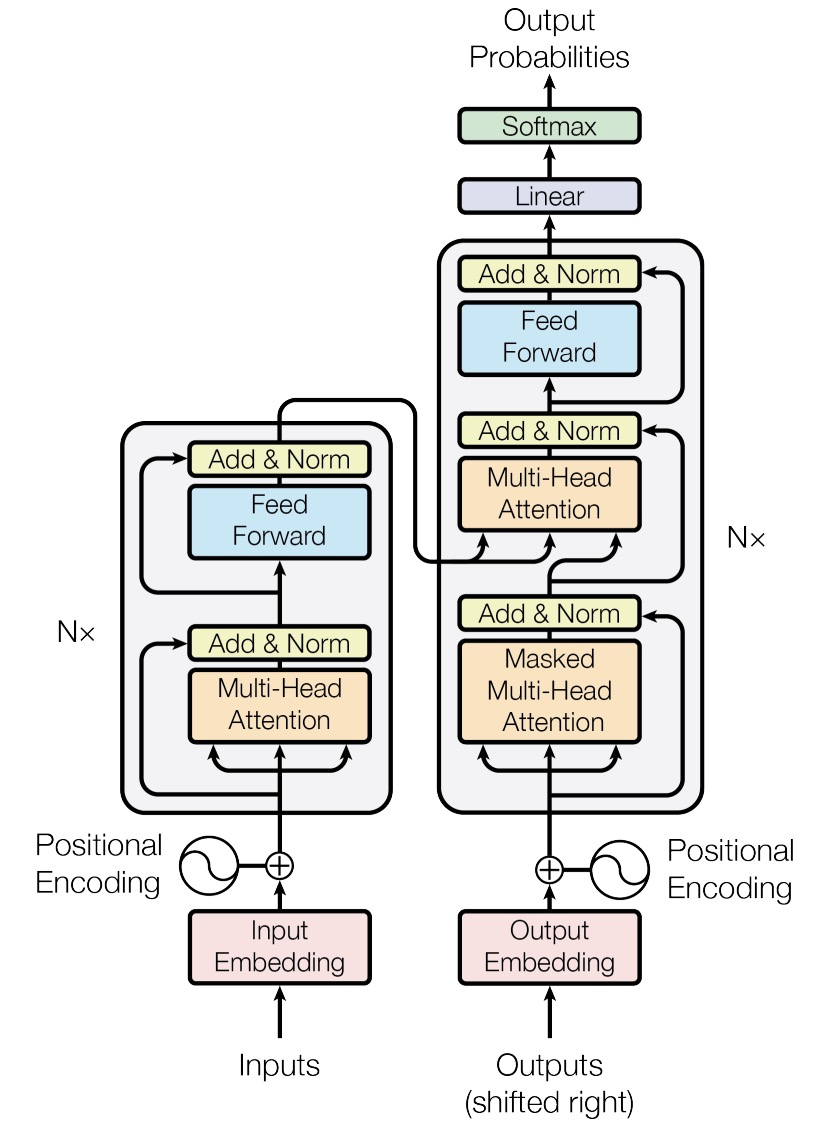
\includegraphics[width=4in]{figures/xulun/transformer.jpg}
  \caption{Transformer 结构框架\cite{vaswani2017attention}。}
  \label{fig1:transformer}
  \end{figure}
  Transformer 是一个基于注意力机制,特别是自注意力机制的模型,
  从根本上摒弃了传统的循环神经网络(RNN)和卷积神经网络(CNN)。
  如\figref{fig1:transformer}, 
  Transformer 模型包含两个
  主要部分:编码器(图左侧)和解码器(图右侧)。这两部分均由数个结构一致的层组成,其
  中每一层都融合了自注意力机制和前馈神经网络。

  \textbf{编码器的介绍}

  Transformer的编码器部分由六个相似的层构成,每层包括两个主要子结构:
  \begin{itemize}
    \item 多头自注意力机制:作为编码器的核心,这一机制使得模型在处理序列中的每个元素时能同时关注其他元素,从而深刻理解整个序列的上下文关系。
    \item 逐位置的前馈网络:这个全连接网络层对序列中每个位置的数据进行独立的线性变换,进一步加强了模型对位置信息的处理能力。
  \end{itemize}
  此外,编码器的每个子层均采用残差连接和层归一化策略,有效防止了深层网络中梯度消失问题的发生,保障了信息的流畅传递。
  
  \textbf{解码器的介绍}

  解码器部分的结构与编码器相似,也是由六个层组成,但在子结构上有所不同,主要包括:
  \begin{itemize}
    \item 掩码多头自注意力机制:与编码器类似,但增加了掩码功能,防止解码器在生成序列时提前获取未来的信息,从而确保了信息生成的时序性。
    \item 编码器-解码器注意力:这一机制使解码器能够关注编码器的所有输出,为序列的生成提供了完整的输入序列上下文。
    \item 逐位置的前馈网络:与编码器的前馈网络相同,它独立处理序列中每个位置的信息。
  \end{itemize}
  解码器的每个子层同样使用残差连接和层归一化,增强了模型的稳定性和训练效率。

  \textbf{缩放点积注意力(Scaled Dot-Product Attention)}

  在Transformer模型中,\textit{缩放点积注意力}(Scaled Dot-Product Attention)起
  着核心作用。它通过计算\textit{查询}($Q$)和\textit{键}($K$)之间的点积,
  来量化序列元素间的关联程度。为了在高维空间中保持梯度的稳定,缩放点积注意力机制将
  点积结果除以\textit{键}的维度$d_k$的平方根进行缩放。其数学表达式为:
  \begin{equation}
      \text{Attention}(Q, K, V) = \text{softmax}\left(\frac{QK^\top}{\sqrt{d_k}}\right)V
  \end{equation}
  其中$V$代表\textit{值}(Value),而softmax函数确保输出的归一化。这种设计使
  得每个元素的输出成为输入值的加权和,其中权重反映了元素间的相关性。
  
  这个机制不仅提升了Transformer在处理长距离依赖问题上的能力,其并行计算特性
  也大大提高了模型的效率。

%\textbf{自注意力机制(Self-Attention)}
%是Transformer结构的基石,它允许模型在处理序列的每个元素时,考虑到序列中的所有其他元素。自注意力的计算公式如下:
%\[ \text{Attention}(Q, K, V) = \text{softmax}\left(\frac{QK^T}{\sqrt{d_k}}\right)V \]
%其中,\(Q\)、\(K\)、\(V\) 分别表示查询(Query)、键(Key)和值(Value),\(d_k\) 为键的维度。

%\textbf{缩放点积注意力(Scaled Dot-Product Attention)}是自注意力机制的一种具体实现,通过缩放因子调整查询和键的点积计算。它提供了一种有效的方法来评估输入元素间的相似度。缩放点积注意力的公式为:
%\[ \text{Scaled Dot-Product Attention}(Q, K, V) = \text{softmax}\left(\frac{QK^T}{\sqrt{d_k}}\right)V \]

\textbf{多头注意力(Multi-Head Attention)}

多头注意力机制是Transformer架构中的一个关键创新,它的设计旨在使模型能够同时从
不同的表示子空间捕获信息。这一机制的核心在于,它不是单一地应用注意力机制,而是将其
分解为多个并行的``头'',每个头独立地关注输入数据的不同方面,从而提高了模型整体的处理能
力和灵活性。

在多头注意力机制中,每个头都独立地执行缩放点积注意力的操作。这一过程可以分为以下几个步骤:

\textbf{头的分割与独立运算}:输入的查询($Q$)、键($K$)和值($V$)首先被分割成多个头,每个头对应一组不同的权重矩
阵 $W_i^Q$、$W_i^K$ 和 $W_i^V$。这些权重矩阵是模型中的可学习参数,用于将输
入映射到相应的子空间中。其中每个头的计算公式为:
\begin{equation}
\text{head}_i = \text{Attention}(QW_i^Q, KW_i^K, VW_i^V)
\end{equation}

\textbf{缩放点积注意力}:已经介绍过。在每个头中,我们对映射后的查询、键和值执行缩放点积注意力计算。
这包括计算查询和键的点积,根据键的维度进行缩放,应用softmax函数获取注意力权重,最后用
这些权重加权求和值。

\textbf{拼接与输出映射}:计算完所有头的缩放点积注意力后,将它们的输出拼接起来,
再通过一个额外的权重矩阵 $W^O$ 进行映射,得到最终的输出:
\begin{equation}
\text{MultiHead}(Q, K, V) = \text{Concat}(\text{head}_1, \text{head}_2, \dots, \text{head}_h)W^O
\end{equation}

多头注意力机制的引入,使Transformer模型能够同时捕获序列的不同特征(如语法、语义等),
并处理各种复杂的依赖关系。这种机制的优势在于其并行性和灵活性,使得模型在处理复杂的序列任
务时更加高效和准确。

通过这种细致的解释,我们可以更深刻地理解多头注意力机制的工作原
理及其在Transformer模型中的重要作用。这种机制不仅是Transformer的核心创新之一,
也是推动当前自然语言处理领域发展的关键技术。

%多头注意力机制通过将自注意力分解为多个``头'',在不同的表示子空间中并行执行,从而捕捉输入数据的多样化特征。多头注意力的计算公式为:
%\[ \text{MultiHead}(Q, K, V) = \text{Concat}(\text{head}_1, \text{head}_2, \dots, \text{head}_h)W^O \]
%其中,每个头 \(\text{head}_i\) 的计算为 \(\text{Attention}(QW_i^Q, KW_i^K, VW_i^V)\),\(W_i^Q\)、\(W_i^K\)、\(W_i^V\) 和 \(W^O\) 是模型中的可学习权重矩阵。
%
%Transformer模型通过其创新的自注意力机制和编码器-解码器架构,为处理复杂的自然语言任务提供了强大的工具。

\subsubsection*{2) Transformer的衍生模型}

随着NLP技术的不断进步,Transformer的衍生模型,如BERT、GPT、XLNet和RoBERTa,
将Transformer结构与无监督学习结合,
可以在不同NLP任务上实现前所未有的性能,无需每个任务重新训练。
这些模型可根据使用的Transformer结构分类:

\begin{equation*}
  \text{衍生模型} \left\{
      \begin{array}{l}
        \text{Encoder模型(如BERT、RoBERTa),称为自编码模型。} \\ 
        \text{Decoder模型(如GPT、XLNet),称为自回归模型。}
      \end{array}
  \right.
\end{equation*}




\subsubsection*{Encoder模型}

Encoder 模型只使用 Transformer 模型中的 Encoder 模块,也被称为
自编码(auto-encoding)模型。在每个阶段,注意力层都可以访问到原始输入
句子中的所有词语,即具有``双向''注意力。
Encoder 模型通常通过破坏给定的句子(例如随机遮盖其中的词语),
然后让模型进行重构来进行预训练,最适合处理那些需要理解整个句子语义的任务,
例如句子分类、命名实体识别(词语分类)、抽取式问答。
BERT 是第一个基于 Transformer 结构的纯 Encoder 模型,它在提出
时横扫了整个 NLP 界,在流行的 GLUE 基准上超过了当时所有的最强模型。
随后的一系列工作对 BERT 的预训练目标和架构进行调整以进一步提高性能。
目前,纯 Encoder 模型依然在 NLP 行业中占据主导地位。下面简略介绍一下 
BERT 模型及它的变体RoBERTa。

\subsubsection*{BERT 模型}

BERT是基于 Transformer 架构的自然语言处理模型。它采用 Transformer 的编
码器部分来学习文本中单词或子单词之间的上下文关系。与传统的单向模型不同,
BERT 的编码器一次性读取整个单词序列,因此,虽然通常被描述为``双向''模型,
但更准确地说,它是非定向的。

BERT 的训练涉及两种主要策略:Masked LM (MLM)和Next Sentence Prediction (NSP)。
Masked LM (MLM)是在输入序列中随机选择大约15\%的单词并用特殊的[MASK]标记替换,然
后模型尝试预测这些被遮盖的单词。这需要在编码器的输出顶部添加一个分类层,并且通过词嵌入矩
阵将输出向量转换为词汇量,最后使用 softmax 函数计算每个单词的概率。BERT 的损失函数
仅考虑遮盖值的预测。

Next Sentence Prediction (NSP)策略是BERT 接受成对的句子作为输入,并学习预
测第二个句子是否逻辑上紧跟在第一个句子之后。在输入中,50\%是连续的句子对,另一
半则是随机的句子对。在输入模型之前,每个输入序列的开始位置会添加一个特殊的[CLS]标记,
每个句子的末尾添加[SEP]标记,同时引入句子嵌入和位置嵌入。为了预测第二个句子是否跟随
第一个句子,模型将[CLS]标记的输出转换为一个二维向量,并使用 softmax 计算其为连续句子的概率。

BERT 在多个基准测试上取得了显著的成绩,包括 
GLUE、SQuAD、SWAG\cite{zellers2018swag}、CLOTH\cite{xie2018large}、
DREAM\cite{sun2019dream}和 SQuAD 2.0。
BERT 通过这种方式,在理解语言的多个方面,尤其是上下文理解方面,取得了新的突破。然而,由
于其复杂的结构和依赖于大量数据的特点,BERT 在一些情况下难以解释,并且在处理特定类型的
语言数据时可能存在泛化问题。尽管如此,BERT 仍然是自然语言处理领域的一个重要里程碑,并
为后续的模型如 XLNet、RoBERTa 等奠定了基础。

\subsubsection*{RoBERTa 模型}
RoBERTa 模型代表了在深度学习和自然语言处理领域中对
BERT模型的一个重要的进化步骤。这种进化不仅基于对BERT潜力的深入挖掘,而且体
现了对预训练语言模型的深刻理解。在这一过程中,RoBERTa的开发者们采用了四个创
新和优化措施,旨在全面提升模型的性能和适应性。

首先,关于数据集的扩展和训练时长的增加,这些改变源于一个核心理念:更多的数据和
更长的训练周期能够使模型捕捉到更为复杂和微妙的语言模式。通过将数据量从BERT的16GB增
加到160GB,并将训练迭代次数从100K提升至500K,RoBERTa能够在更广泛和多样化的文本上学
习,从而提升其对于复杂语言结构的理解能力。

动态掩码的引入是RoBERTa另一个创新之处。与BERT的静态掩码不同,RoBERTa在每个epoch
中对文本采用不同的掩码模式。这种方法有效防止了模型对固定掩码模式的过度适应,从而推动模型
学习更加泛化的语言表示。具体而言,这种动态掩码策略是在训练过程中实时应用的,确保即使同一
文本在不同的训练阶段也会呈现出不同的掩码模式,增加了训练的多样性和复杂性。

此外,去除BERT中的下一个句子预测(NSP)任务也是一个关键决策。尽管NSP被设计来提高模型
对句子间关系的理解,但研究发现,在去除这一任务后,RoBERTa在多项下游任务中的表现有了显
著提升。这表明对于模型的优化,有时候减法也是一种有效的策略。

再者,RoBERTa在训练中对样本长度的处理也展示了其对复杂语言模式理解的重视。通过在训
练中始终使用全长(512个令牌)的序列,RoBERTa强化了对长距离依赖关系的学习,这对于
处理更为复杂的语言结构至关重要。

这些改进使得 RoBERTa 在多个基准测试(如 GLUE、RACE\cite{lai2017race}、SQuAD 等)
中取得了领先性能,甚
至超过了人类的表现。
综合来看,RoBERTa的这些创新和优化措施共同构成了其卓越性能的基础。通过在大规模数据
集上进行深入训练,实施动态掩码机制,精简训练任务,以及优化样本长度处理,RoBERTa不仅
巩固了BERT作为一种强大的语言模型的地位,也为后续的NLP研究提供了宝贵的参考和启示。


\subsubsection*{Decoder模型}
Decoder 模型只使用 Transformer 模型中的 Decoder 模块。在每个阶段,对
于给定的词语,注意力层只能访问句子中位于它之前的词语,即只能迭代地基于已经生
成的词语来逐个预测后面的词语,因此也被称为自回归(auto-regressive)模型。
下面就简要介绍一些常见的Decoder 模型。

\subsubsection*{GPT 模型}
GPT 模型是第一个使用了Transformer架构进行预训练的大型语言生成模型。这个模型标志着自然语言处
理中一个重要的转变点。
GPT 结合了 Transformer Decoder 架构和迁移学习方法,
在大量开放在线数据上进行无监督预训练,特别是在 BookCorpus 数据集上。
其预训练任务是根据上文预测下一个单词,从而使模型能够在没有限制的情况下学习语言特征。
此外,GPT 还通过微调适应各种下游任务,如文本蕴含、语义相似性、情感分析等,在包括
SNLI、MNLI、ROC、COPA 和 GLUE 等多个 NLP 基准
测试中取得了显著效果。

然而,GPT 也存在一些局限性,比如它主要使用单向(向前)自注意力机制,这意味
着在处理文本时,每个词只能看到它前面的词,这限制它对上下文的理解。

\subsubsection*{XLNet 模型}
XLNet 模型也基于Transformer Decoder架构,但采用了双向
(或更准确地说是排列敏感的)上下文处理。XLNet通过排列语言
建模(Permutation LM)来同时学习文本的前向和后向依赖。
XLNet的出现在自然语言处理领域引发了显著关注,特别是它在
特定任务中相较于BERT的显著性能提升,标志着NLP模型发展的一个新阶段。这种
模型不仅继承了自回归语言模型的强大特性,同时也融合了自编码语言模型(如BERT)的优
势,创造了一种新的、更为复杂和有效的预训练机制。

XLNet的核心在于它的创新性预训练目标——排列语言模型。在
BERT中,模型预训练是通过随机选择一些单词并将其替换为[MASK]标记来进行的,
然后模型被训练来预测这些被掩盖的单词。然而,这种方法导致了一个问题:在实
际应用中,即微调(fine-tuning)阶段,输入数据中并不存在[MASK]标记,这可
能导致预训练和微调之间的不一致性。
为了解决这个问题,XLNet引入了排列语言模型。在这种模型中,对于一个给定长度
的句子,模型会考虑所有可能的单词排列组合。在每次训练迭代中,
模型会随机选择一种排列,并基于这种排列来预测单词。具体来说,对于一个句子中
的每个位置,
模型尝试预测这个位置的单词,给定在这个特定排列中它之前的所有单词。
这种方法有效地模拟了自回归(autoregressive)语言模型的特性,
同时也使模型能够在预训练中学习到上下文的全面信息。

在与BERT的比较中,XLNet的预训练机制展现出三个独特的优势:
首先,BERT通过在输入中随机遮盖某些词并预测这些词来进行训练,而
XLNet则采用了无需明显[MASK]标记的内部随机``遮盖''单词方法。这种差异使得
XLNet在预训练和微调阶段保持了更高的一致性,解决了BERT预训练与微调不一致的问题。

此外,XLNet在处理生成型任务上也表现出明显的优势。得益于其自回归特
性,XLNet能够在维持自然的从左到右的生成过程的同时,内部隐含上下文信
息,这对于生成连贯、流畅的文本尤为重要。

针对长文本的处理能力也是XLNet的一个亮点。它整合了
 Transformer XL\cite{dai2019transformer} 的技术,使
得在处理长文档类型的NLP任务时,相比BERT有着更为显著的优势。

总的来说,XLNet通过结合自回归和自编码语言模型的优势,通过其排列语言模型和注
意力掩码机制,有效地利用上下文信息。这些特性使得XLNet在多项NLP任务中,尤其是在
生成型任务和长文档处理方面,相较于BERT展现出更加卓越的性能。这种创新的预训练方法
不仅解决了先前模型的某些局限性,也为未来NLP模型的发展提供了新的方向。


\subsection{推理模型鲁棒性研究}
\label{sec1:robustness}
上一小节是我对我所研究的相关的推理方法的介绍,尽管大型预训练语言模型在NLP
领域取得了显著进展并
在现实世界中得到了广泛应用,
但它们在处理领域外数据、抵御对抗性攻击\cite{mccoy2019right,jin2020bert}以及应对输入的微
小扰动\cite{ebrahimi2018hotflip,belinkov2018synthetic}方面仍显脆弱。这些局限性
可能会阻碍这些模型在实际环境中的安全部署,并影响用户对NLP模型的信任度。为了应对这些
挑战,语言技术领域的研究者们正加大力度,旨在深入理解并解决这些鲁棒性问题。
在这一节中,我们将进一步讨论自然语言推理任务中模型鲁棒性的相关研究。
%接下来是对这些模型在具体任务上的鲁棒性的探究的相关工作,
包括模型的鲁棒性的测试和提高模型鲁棒性的相关方法。

\subsubsection{鲁棒性的定义和评估方法}

Wang等人(2022)\cite{wang2022measure}对模型的鲁棒性进行了定义:

\begin{definition}[鲁棒性]
在自然语言处理模型中,\textbf{鲁棒性}指的是模型在面对不同分布的测试数据时保持性能的能力。
具体来说,对于一个输入 $x$ 和它的正确标签 $y$,对于一个在 $(x, y) \sim D$ 上训练的模型 
$f$ 及其对 $x$ 的预测 $f(x)$,鲁棒性是通过模型在测试数据 
$(x', y') \sim D'$(可能与 $D$ 分布不同)上的表现来衡量的。
通常使用诸如鲁棒准确率这样的指标来量化鲁棒性,
定义为 $E_{(x', y') \sim D'}[f(x') = y']$。
\end{definition}

在探讨模型鲁棒性的文献中,可以粗略地将他们分为两类:对抗性攻击下的鲁棒性和分布偏移下的鲁棒性。
对抗性鲁棒性关注在输入 $x$ 周围创建微小扰动 $\delta$ 形成 $x'$ 时模型的表现,
而分布偏移鲁棒性关注在自然发生的不同分布上的模型表现。
这些分类共同探讨 $D'$ 是合成分布偏移(如对抗性攻击)还是自然分布偏移。

\textbf{对抗性攻击下的鲁棒性}:
对抗性鲁棒性的研究主要集中在模型对输入的微小扰动($\delta$)的反应上,
即在原始输入 $x$ 周围引入扰动,形成 $x'$,并观察模型的响应。这类攻击通常通过添加
对人类几乎不可察觉的噪声,以欺骗模型做出错误判断。这种策略最初在计算
机视觉领域被广泛研究\cite{szegedy2014intriguing,goodfellow2014explaining},
随后扩展到自然语言处理领域\cite{Marco2020acl,tan2020s,schwinn2023exploring,boucher2022bad},
凸显了对NLP模型进行全面鲁棒性评估的重要性。

\textbf{分布偏移下的鲁棒性}:
与之相对,分布偏移下的鲁棒性关注模型在不同自然分布的数据上的表现。
这类研究反映了现实世界数据多样性和复杂性的影响,如语法错误、方言、
语言差异等因素\cite{blodgett2016demographic, demszky2021learning},以及
同一任务在不同领域的新数据集上的表现。


CheckList\cite{Marco2020acl}是一个结合了对抗性攻击和分布偏移下鲁棒性测试的方法论。
它借鉴软件工程中的``黑盒测试''方法,重点评估NLP模型在不同输入变化下的表现。这一方法论包括三
个核心部分:功能评估、测试方法和测试用例生成。

1)功能评估:此部分更多关注模型在处理各种NLP任务(如语义角色标注、命名实体识别等)时的能力,
为后续的鲁棒性测试奠定基础。

2)测试方法和测试用例:这里包括对抗性攻击下的鲁棒性和分布偏移下的鲁棒性两个方面。
对于前者,CheckList通过模拟对抗攻击中的微小变化或扰动(如情感分析中的句子轻微修改),
评估模型的反应\cite{goodfellow2014explaining}。它通过不变性测试(INT)和定向期望测试(DIR)等方法,
检验模型在处理对抗性攻击下的鲁棒性(如语法结构变化、情感强度变化)时的稳定性。同时在分布偏移的鲁棒性的测试中,
CheckList通过模板方法简化了大量有效测试用例的创建。
例如,可以创建一个模板``我\{NEGATION\}\{POS\_VERB\}这个\{OBJECT\}'',
并通过不同的词语组合生成多个测试句子,如``我不喜欢这个电影'',来评估模型对否定构造的处理能力。这些例子的主题和分布与原来的测试集已经完全不同。

总结来说,CheckList为NLP领域提供了一个全面的框架,
用于评估和提升模型在面对对抗性攻击和分布偏移时的鲁棒性。
这不仅有助于揭示模型的潜在薄弱环节,也为提高模型的整体鲁棒性提供了实践指导。

\subsubsection{提升推理模型鲁棒性的方法}
在自然语言推理的领域中,关键的目标之一是增强模型的鲁棒性。为此,我们通常采
用两种主要策略:一是数据增强技术,用于丰富训练材料;二是优化模型架构和训
练流程,以提升模型的内在强度和适应能力。

1) 数据增强,作为优化大规模神经网络模型性能的核心策略,
在自然语言处理领域的应用尤为关键。我们概述了几种主要的文本数据增强技术及其在学术研究中的应用,
展示了它们如何为自然语言推理任务带来显著的性能提升。

\textbf{回译(Back-translation)}\cite{sennrich2016improving,edunov2018understanding,xie2020unsupervised}:
通过将文本从一种语言翻译到另一种语言,再翻译回原语言,创造出文本的新变体,从而增加数据的多样性。

\textbf{c-BERT词替换}\cite{wu2019conditional}:
运用BERT模型来识别并替换文本中的关键词汇,生成文本的新版本,以此来丰富语料库。

\textbf{混合(Mixup)}\cite{guo2019augmenting,chen2020mixtext}:
通过在不同文本样本之间进行线性组合,创造全新的文本实例。

\textbf{截断(Cutoff)}\cite{shen2020simple}:
分为两类,第一类叫做Token截断,即随机选取Token,将对应Token的嵌入整行置零;第二类是特征截断,
即随机选取嵌入的特征,将所选特征维度整列置零。

2) 优化模型架构和训练流程的方法,一般指的是调整模型结构来增强模型在自然语言推理任务当中的鲁棒性。
最常用的方法是\textbf{对抗性训练}\cite{zhu2019freelb,jiang2020smart},
这种方法通过在词嵌入层引入微小的扰动,合成附加样本,提高模型对异常输入的鲁棒性。
该方法通过梯度反传生成对抗性扰动,并加到原始嵌入矩阵上,产生增强样本,
通常应用于有监督训练场景。

在Qu(2020年)\cite{qu2020coda}的研究中,通过比较这些模型增强技术
在RoBERTa模型上处理自然语言推理任务(MNLI)的效果,发现回译和对抗性训练在提升模型
性能方面效果显著,明显优于c-BERT、混合和截断技术。因此,将回译作为自然语言推理任务中的一
种强有力的基准进行数据增强方法比较,是一种合理的策略。这些研究成果不仅强调了数据增强在提
升模型性能方面的重要性,还为选择适当的数据增强策略提供了宝贵的指导。

\subsection{推理模型可解释性研究}
\label{sec1:interpretability}

\subsubsection{推理模型鲁棒性不足的现象}

在本节中,我们聚焦于推理模型在处理常识性推理任务时所表现出的鲁棒性不足问题。虽
然这些模型在标准测试环境中取得了显著成就,但它们在遭遇对抗性数据或与训练环境
显著不同的场景时,却显露出不足\cite{naik2018stress,mccoy2019right,schuster2019towards,nie2020adversarial,Marco2020acl}。

以CheckList\cite{Marco2020acl}为例,该研究通过对模型进行重新测试,涵盖
了多种不同能力,结果显示模型性能与原始测试结果相比有显著
差异。这一发现揭示了模型在鲁棒性方面的严重不足。然而,尽管CheckList在揭露
模型学习过程中的一些缺陷上取得了进展,比如在``语义角色标注''等任务下的表现,
它却未能深入分析导致模型鲁棒性不足的根本原因。

\subsubsection{推理模型鲁棒性不足的原因的探究}

在深入探究推理模型鲁棒性不足的问题时,关键在于分析模型处理信息的方式和焦点。
一种常见的假设是,这些模型可能过于专注于数据的特定结构元素,例如,它们可能
只关注\textit{前提}-\textit{假设}关系对中的\textit{假设},而忽视了前提与假设之间的逻辑联系。这种假设揭示了一个更深层
次的问题:模型可能主要学习了数据中的
统计偏差\cite{naik2018stress,mccoy2019right,schuster2019towards,nie2020adversarial},
也就是所谓的偏见线索(bias cues)或虚假线索(spurious cues)。

这种现象的根源在于数据集的构建方式。由于数据集的特定特征或模式,模型往往不是
学习解决问题的通用策略,而是学习特定于该数据集的简化规则。举个例子,在自然
语言处理任务中,如果某个数据集中绝大多数标记为``正确''的样本都包含某个特定的词汇,模型
可能就会简单地依赖这个词汇来做出判断,而没有真正理解句子之间的逻辑关系。这种简化的
学习方式使模型在面对结构或上下文有所不同的新数据时显得脆弱,无法有效适应或正确解释。
如果这种线索刚好在\textit{假设}部分,
那可能就会造成模型只关注\textit{假设}部分。

因此,探究推理模型的鲁棒性不足,我们不仅要关注模型本身的处理机制,也需要深入理解数据
集构建的影响。


\subsubsection{推理模型鲁棒性不足的原因的验证}

在前面探讨推理模型鲁棒性不足的原因时,研究人员提出了一个关键假设:
模型可能过分专注于数据的特定结构元素,如仅关注推理任务中\textit{假设}部分而忽略了\textit{前提}。
为了验证这个假设,研究者们开发了``仅假设''测试\cite{gururangan2018annotation}和注意力图\cite{vig2019multiscale}这两种方法,
旨在深入分析验证和量化此现象。

\subsubsection*{仅假设测试}

``仅假设''测试的核心思想是检验模型在仅凭假设(即问题或选项本身)的情况下的表现。
这种测试通常用于评估自然语言理解模型。在这种测试中,模型只被提供假设部分,而没
有相应的前提或上下文信息,比如在 \secref{sec1:challenge} 中提到的SNLI的例子,只提供假设
``A man is pushing a baby carriage'' 而不提供前提,让模型猜测前提跟假设之间的关系。
从人的角度来看,
解决这个问题是不可能的,因为问题本身有缺陷,很难做出选择,但是如果模型依然做出跟有前提时一致的结果,
研究者就可以判断模型可能过度依赖于假设中的某些关键词或短语,而忽
略了理解整体意义所必需的上下文。

这种方法的主要优势在于能够揭示模型潜在的缺陷:模型可能
仅依赖假设中的关键信息来作出判断,而不是实现全面的理解。然而,其局限性
在于它不能完全展现模型在处理真实场景时的推理模式。这是因为模型在训练阶段所
依赖的数据包含了前提,而在测试时使用的数据结构却与之不同,仅包含假设而无前提。这
种结构变化导致的差异和信息损失是该方法无法克服的。

\subsubsection*{注意力图}

注意力机制是深度学习中的一种重要技术,它帮助模
型聚焦于输入数据的关键部分。注意力图是一种可视化工具,它展示
了模型在做出决策时对不同输入部分的关注程度。通过观察这些图,研究者
和开发者可以更直观地理解模型的决策过程,识别模型关注的是哪些信息。

然而,注意力图的直观性并不总是代表其可靠性或准确性。
研究\cite{jain2019attention}指出,即使模型通过注意力机制
突出显示的部分,也可能并不准确地代表模型决策的真实依据。这表明,
尽管注意力图提供了一个理解模型决策过程的窗口,但它不应被视为模
型内部工作机制的完整映射。

虽然``仅假设''测试和注意力图作为工具在解析和评估模型行为方面扮演着关键角色,
但它们的分析深度有限。这些方法虽然能在一定程度上揭示模型中的偏见,但在深入探讨数
据中的偏见如何影响模型的核心机制方面,仍显不足。因此,对数据偏见如何具体作用于模型
的机制进行深入研究,已成为当前一个亟待解决的重要课题。



\subsection{本章小结}

在本章中,我们全面而深入地探讨了常识性推理领域的核心要素。章节始
于对该领域的基本任务和评估标准的深度分析,揭示了其核心内容、目标和所面
临的挑战。随后,我们对推理模型的发展历程进行了细致的梳理,从符号方法、早
期统计方法,一直到神经网络方法,并对这些方法的优势和局限性进行了详尽的讨论。特
别地,对于常识性推理中的神经网络方法,我们进行了深入的阐述,这些方法和模型将在后
续章节中反复出现和引用。

章节接下来转向推理模型鲁棒性的研究,详细探讨了鲁棒性的定义、测试
方法,以及提升模型鲁棒性的多种策略。我们对模型在处理多样化和对抗性
数据时的挑战进行了深入的剖析,并探索了增强模型适应性和鲁棒性的有效方法。
最终,本章还深入讨论了推理模型的可解释性研究,特别是模型鲁棒性不足的表现、原
因的假设以及这些假设的验证方法。

综合来看,本章旨在为读者提供一个全景式的视角,深刻理解常识性推理领域的最
新研究趋势和发展,包括其核心任务、评估基准、方法论以及鲁棒性和可解释性研究的最新进展。

\newpage
\null
\newpage

\newpage
\fancyhead[LH]{上海交通大学学位论文}
\fancyhead[RH]{第三章\quad 基于知识增强的常识性推理研究}
\setcounter{figure}{0}
\setcounter{table}{0}
\section{基于知识增强的常识性推理研究}
在本研究中,我们致力于解决常识推理领域的关键挑战:增强模型的常识性推理能力。
在\secref{sec1:related}中,我们已经深入探讨了当前领域内的领先技术,特别是BERT等先进
的神经网络方法。尽管神经网络在常识推理任务中已显示出卓越的性能,
但根据Lin等人的研究\cite{lin2020birds,peng2022copen},在精确处理和表达常识性知识方面,
这些方法仍有进一步提升的空间。

针对这一挑战,我们选择了一个具有挑战性的任务作为研究重点:预测叙事故事的结局。这一
任务的灵感源自早期的故事理解研究\cite{meehan1977tale},并随时间演进,扩展为预测故
事中可能事件的任务\cite{chambers2008unsupervised}。我们的实验是在ROC故事填
空测试数据集\cite{mostafazadeh2016corpus}上进行的,这一数据集为我们提供了评
估模型性能的有效平台。

为了在这一领域实现突破,我们提出了一种注重故事中关键概念识别与
优化的新方法。这种方法通过专注于故事的关键元素,而非全体词汇,旨在简化句
子结构,减少干扰信息,从而提升模型在捕捉故事核心内容方面的效能。此外,我们
采用了一种将结构化的常识知识融入句子表达的策略,通过结合结构化预训
练的概念嵌入(embedding),增强
了模型在理解故事情境与结局之间关键概念联系的能力。

通过将这些精细化的概念与丰富结构化知识相结合,我们不仅深化了对故事情节的理解,
也在故事推理任务的准确度上取得了显著的提升。这一成果标志着我们在常识推理任务
处理方面迈出了重要的一步。

\subsection{概述}
\label{sec2:intro}
在叙事故事中预测``接下来会发生什么''是人工智能中常识推理的一个重要并且富有挑战性的任务。
故事理解最初在规划和目标搜索的背景下被研究~\cite{meehan1977tale},这是人工智能中最重要的问题之一。
随着研究的深入,这一任务逐渐演变为预测故事中可能接踵
而至的事件~\cite{chambers2008unsupervised}。众多研究聚焦于一个标准数据集
——故事填空测试(ROC)~\cite{mostafazadeh2016corpus}。这个挑战要求从两个备选
结局中选出一个与四句话故事情境最为吻合的结局,如\figref{fig:story}(a)所示。

\begin{figure}[th]
  \centering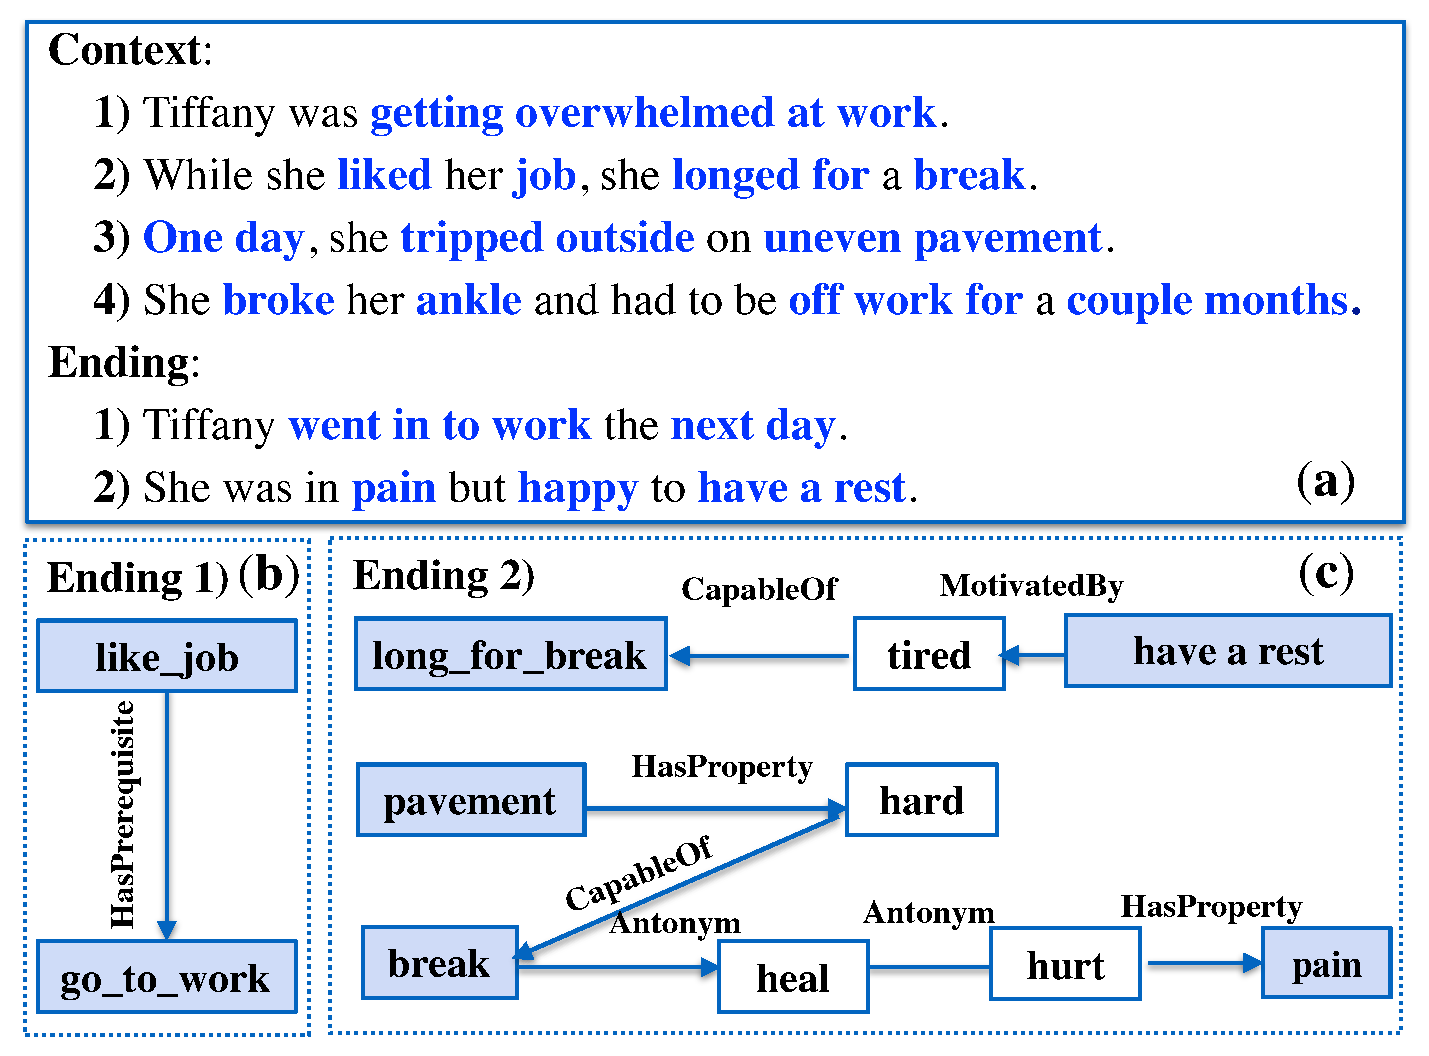
\includegraphics[width=4in]{figures/story/story_example}
  \caption{故事填空任务中的一个例子。在(b)和(c)中,蓝色框内的单词代表故事中的关键概念;白色框内的单词虽非故事概念,但作为桥接节点发挥作用。}
  \label{fig:story}
  \end{figure}

先前的研究成果表明,结构化的常识知识对于深化故事理解颇具
帮助~\cite{li2019story}。例如,观察\figref{fig:story}(b)和(c),我们
不难发现,结构化知识有助于通过分析词汇间的逻辑联系来推断故事的
可能结局。更有趣的是,仅凭
借关键词(在图中以蓝色高亮显示)就能做出推理,这些词汇在推理过程中提
供了丰富信息,而无需解析全文。相对而言,其他未突出显示的词汇不仅信息量较少,
甚至可能由于其模糊的语义而对分类器造成干扰。例如,``Tiffany''这一名字常与珠宝相关联,
将这层含义引入故事情境中,往往会产生负面效果。

受以上观察的启发,我们从两个方面运用常识知识来优化故事的表达方式。
首先,我们通过从ConceptNet~\cite{speer2017conceptnet}中提炼关键概念,对
句子进行简化处理。ConceptNet作为一个社区策划的开放领域知识图谱,涵盖了绝大多数
常识推理所需的知识,从而实现了{\em 句内}概念的有效表示。其次,我们通过
融入ConceptNet知识图谱中的预训练概念嵌入,将结构化的常识知识引入故事句
子的表达中。例如,在\figref{fig:story}(c)中,``long for break''与``have a rest''之间
通过{\em CapableOf}和{\em MotivatedBy}关系边相连。这些连接为我们在故事中``串联起关键点'',帮
助我们进行更加深入和有意义的推理分析。

%在面对常识推理任务中的首个挑战(\ref{sec1:challenge}节):提升模型常识性推理能力的挑战时,
%本研究聚焦于当前最为前沿的方法——神经网络方法(\ref{sec1:approachs}节),
%并对其进行了深入分析。尽管神经网络在常识推理任务中表现出色,
%但有工作\cite{lin2020birds}指出,在处理常识性知识时,这些方法仍有改进空间,
%特别是在准确把握和表达常识性知识方面。为了在这一领域取得进一步突破,
%我们选择了一个具有挑战性的任务——``预测叙事故事结尾''。
%这一任务源自早期关于故事理解的研究\cite{meehan1977tale},
%后演变为预测故事中可能发生事件的任务\cite{chambers2008unsupervised}。
%本研究在 ROC 数据集\cite{mostafazadeh2016corpus},也就是故事填空数据集,
%上进行了实验评估,该数据集要求从两个备选结局中选择一个与四句话故事情境最为契合的结局。

%最初的故事填空测试尝试主要集中在计算候选结局与故事情境句子间的语义相似度上。
%这通常需要对故事句子进行某种形式的表示,如通过平均句子中的词
%向量\cite{mikolov2013distributed},应用sentence2vec\cite{kiros2015skip},
%DSSM\cite{huang2013learning}或其他特征\cite{schwartz2017story}。近期的方法
%更倾向于采用两层架构:首先使用LSTM\cite{hochreiter1997long},GPT\cite{radford2018improving}或BERT\cite{devlin2018bert}等预训练语言
%模型从庞大的语料库中构建每个句子的表示,然后在ROC数据集上对分类模型进行微调,
%以融合成完整的故事情境表示。



%在这些方法中,故事的完整句子被采用。早期模型对
%句子中的每个单词平等对待,而后续更先进的语言模型,如基于
%注意力机制的模型,为不同单词赋予了不同的权重。这些权重通常是从
%大型语料库中隐式学习得到的,而常识性知识在其中虽然存在,但相对稀
%疏。从\figref{fig:story}(a)中可以看出,通过专注于关键词(用蓝色高亮表示)而
%非所有单词,可以更准确地找到正确的结局。实际上,其他未高亮的单词可能因其
%模糊不清的含义而干扰下游分类器。例如,提及``Tiffany''这个名字可能会误导读者
%联想到珠宝,从而对故事情境产生不利影响。

%基于这些观察,我们提出在使用语言模型表示之前,通过保留被认为重
%要的标记来简化句子,即将不重要的标记的权重降至零。我们将句子建模为一系列
%事件和概念,这些概念在ConceptNet\cite{speer2017conceptnet}中有定义,
%一个社区策划的开放领域知识图谱,包含了大量常识推理所需的知识。ConceptNet的优势在
%于:i)事件和概念以简单短语的形式定义,无需复杂的结构,便于运
%行时匹配;ii)概念间的关系由人类定义,从而更为准确。如\figref{fig:story}(a)所示,
%每个蓝色短语(多词表达)都与ConceptNet中的某一概念相匹配,共同构成理解故事的
%关键要素。这种方法虽简单,但直观有效。在本研究中,我们从两方面利用常识知识来改进故事表征。

%首先,我们通过从句子中提取一系列ConceptNet概念来简化每个句子,
%从而获得\textbf{句内}概念表征。通过简化句子,我们实质上减少了
%训练数据中的噪音和变化,使得即使在有限的数据量下也能获得更好的性能。
%接着,我们使用来自大型语料库的预训练语言模型来获取每个简化句子的语义表
%征。我们采用了在故事结局推理任务上取得良好成绩的典型编码
%方法\cite{roemmele2017rnn,mostafazadeh2016corpus,devlin2018bert},并
%将展示简化如何显著提高这些编码方法的准确性。

%其次,我们通过将故事句子表征与预训练的概念嵌入结合,将ConceptNet中的
%结构化常识知识纳入其中。这些嵌入编码了存在于ConceptNet知识图谱中的关键概念之
%间的关系,如故事情境和结局之间的联系。例如,在\figref{fig:story}(c)中,
%``long for break''与``have a rest''之间通过\textit{CapableOf}和\textit{MotivatedBy}关系相联系。
%这些关系边缘帮助我们在故事中``串联起关键点'',
%从而使我们能够沿着故事情节进行更深入、更有意义的推理。

尽管已有的方法在故事结局预测任务上的研究取得了显著进展,但这些成果多是基于
原始ROC数据集的验证分割实现的。已有研究表明,验证集可能受到注释偏差的影
响\cite{gururangan2018annotation,sharma2018tackling},这意味着其中包含
的统计特征可能会被学习,而不需要真正理解故事。因此,在本研究中,我们未使用验证集,
而是创建了一个新的训练集,与测试集之间不共享统计线索,从而最大限度地减少训练与测
试之间的信息泄露。

本研究的主要贡献是在常识性推理领域引入了一种创新且有效的方法论。我们实施
了一种精心设计的句子简化策略,专注于故事中关键概念的提炼。这种方法不仅
降低了模型处理的复杂性,而且通过集中处理核心信息,极大地提高了模型捕捉
故事情节的精准度。通过将这些精化的概念与ConceptNet数据库中的丰富结构化
知识结合,我们在故事结局预测的准确率上实现了显著的提升。
同时,在实验方法上,我们通过精心筛选和优化的训练数据集来确保了评估的公正性和准
确性。

\subsection{相关工作}
\label{sec2:related}

我们的研究是在故事填空任务的背景下进行的,受到了三个研究领域的启发:
脚本学习、常识性知识,以及文本推理中的标注偏差。接下来,我们将对这些领域进行详细的回顾。

\subsubsection*{故事填空任务}

故事填空任务\cite{mostafazadeh2016corpus}的目的是
为了评估故事理解和常识性推理的能力。众多基准方
法\cite{mihaylov2017story,mostafazadeh2016story}通过
测量情境句子与结局在向量空间中的语义相似度,来评定候选结局的合理性。
可以采用不同的句子表征方法,比如对word2vec的平均\cite{mikolov2013distributed}、
entence2vec\cite{kiros2015skip}和DSSM\cite{huang2013learning}。另外,句子长
度和字符n-gram等风格特征,也在区分正确与错误结局方面发挥作用\cite{schwartz2017story}。

近年来,多种深度学习方法被用于解决ROC任务。这些方法中的大多数遵循两层架构:
首先构建每个句子的表征,然后将其聚合为整个故事情境的表征。句子表征可以通过LSTM、
GRU和注意力层\cite{wang2017conditional,zhou2019story}从词嵌入中得
到,或者通过预训练模型如Sentence2vec\cite{roemmele2017rnn,srinivasan2018simple}和
GPT\cite{radford2018improving,chen2018incorporating}生成。同样地,情境表征可以通
过递归层\cite{cai2017pay}、注意力层\cite{li2018multi}或简单串联\cite{bugert2017lsdsem}对所
有情境句子的语义进行编码。通过结合浅层特征和DNN模型,还可以进一步提高任务的准确性。

\subsubsection*{统计脚本学习}

``脚本''指的是一系列预定、固定模式的事件序列,用以定义特定的活动,它
对文本理解十分重要\cite{chambers2009unsupervised, regneri2011learning, schank1975scripts}。早
期研究\cite{schank2013scripts,mooney1985learning}通过从文本中构建知识
库来学习脚本。近期,研究人员运用统计模型从大量数据中提取不同类型的表示,包括无监督
地学习叙事模式和脚本\cite{chambers2009unsupervised,regneri2011learning},以及
事件模式和框架\cite{chambers2011template,balasubramanian2013generating,sha2016joint,huang2016liberal}。为了推理这些
知识,研究人员试图将事件预测问题转化为语言模型范式\cite{pichotta2014statistical,rudinger2015script,hu2017happens}。对
于故事填空任务,语义语言模型(SemLM)\cite{peng2016two}作为框架级别的语言模型,能够有
效表示事件的顺序语义\cite{li2018multi,chaturvedi2017story}。此外,基于规则
的方法\cite{lin2017reasoning}为给定情境中的显式事件制定了匹配规则。其他
一些工作\cite{modi2014inducing,regneri-etal-2010-learning,modi2016event}则将事
件映射到语义嵌入表示中,这可能导致数据稀疏问题。

\subsubsection*{文本推理中的常识性知识}
在许多推理任务中,常识性知识被证明是非常有效的,如阅读理
解\cite{mihaylov2018knowledgeable}和对话生成\cite{liu2018knowledge}等领
域。最近,ConceptNet已被纳入到ROC模型中。例如,\cite{chen2018incorporating}提出了一
种基于概念嵌入相似度的简单而有效的常识性特征。文献\cite{guan2018story}则通过聚合句子中每
个概念标记相邻的概念嵌入,来扩展每个概念的语义。在我们的研究中,常识性知识的
运用主要表现在两个方面:一是作为简化过程的指导原则,二是作为增强每个句子语义的额外资源。

\subsubsection*{文本推理中的标注偏差}
在多个文本推理数据集中,如SNLI\cite{bowman2015large}和MNLI\cite{gururangan2018annotation},已经
发现存在广泛的标注偏差。一些研究致力于通过人工\cite{sharma2018tackling}或采用
对抗性方法\cite{zellers2018swag}来自动生成具有额外标注的新数据集。文献\cite{roemmele2017rnn}提供了一种生成错误样
本的简单但有效的方法。其他研究则关注于避免偏见的模型\cite{clark2019don,zhao2018gender}。尽管这些
方法可能减少收集新数据集的工作量,但它们难以迁移到其他模型上,这是其主要局限性。

\subsection{基于常识知识增强的故事结局预测框架}
\label{sec2:approach}

\begin{figure*}
  \centering
  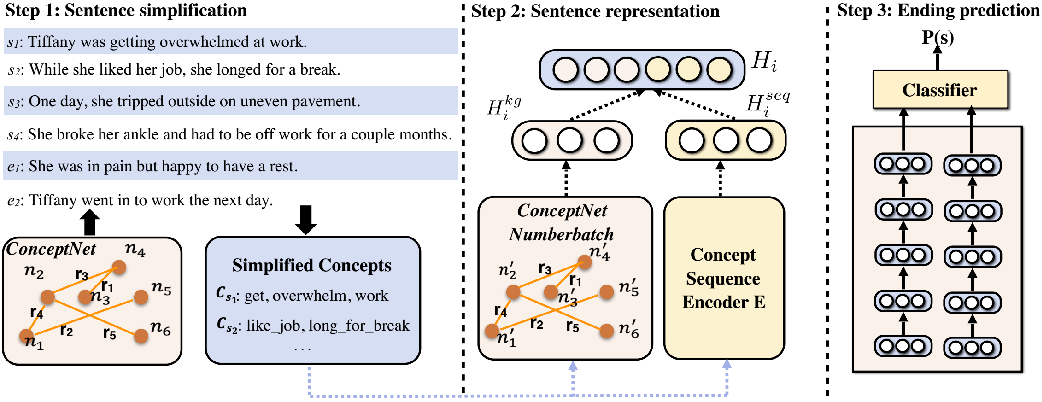
\includegraphics[width=\columnwidth]{figures/story/model}
  \caption{框架概览:我们的框架分为三个主要步骤:句子简化、句子表征和结局预测。${n_1,...n_6}$ 表示ConceptNet中的标记节点,${r_1,...r_6}$ 代表节点间的常识关系。${n_1^{'},...n_6^{'}}$ 是在ConceptNet上训练得到的对应向量。}
  \label{fig:model}
  \end{figure*}

考虑到一个包含$L$个句子 $\textbf{s} = (s_1, s_2, ..., s_L)$ 的故事情境,
我们的任务是从两个候选结局句子 $e_1$ 和 $e_2$ 中预测出正确的结局。
我们提出的方法旨在通过引入ConceptNet中的常识知识,来改进和扩展故事句子的表示,
以便更准确地预测故事结局。如\figref{fig:model}所示,该框架包括以下三个主要步骤:
句子简化(Sentence simplification)、句子表征(Sentence representation)
和故事结局预测(Ending prediction)。

\subsubsection{概念提取与句子简化}
\label{sec2:sentence_simplification}
我们的目标是从包含N个单词的输入句子 $s = {w_1, ..., w_N}$ 中提取
一系列关键概念和事件 $C_s$。我们选择ConceptNet~\cite{speer2017conceptnet} 作为这
些概念和事件的来源,因为它覆盖了广泛的常识知识。ConceptNet中的概念和事件通常由一到两
个单词的短语表达,例如``break ankle''。但在实际语境中,人们可能会使用更多样化的表达方
式,如``break her ankle''。为了弥补这种差异,我们开发了一种模糊匹配启发式方法,允许
在ConceptNet中的概念短语中加入最多 $\lambda$ 个额外单词以便在输入句子中实现模糊匹配。

面临的另一个挑战是,提取的概念可能在输入句子中相互重叠。
例如,从句子``She hope it would come back for more later''中,我们能提
取出``hope''、``\textbf{come back}''、``\textbf{come for}'' 和 ``more''等概念。在
这种情况下,我们将保留所有有意义的概念。随后,我们会从 $C_s$ 中移除那些被其他概念
完全覆盖的重复概念。例如,``come''会被``come back''覆盖,因此从列表中删除。

完整的简化算法展示在 \algoref{alg:simplify} 中,其中 $|c|$ 表示
概念 $c$ 包含的单词数量。

\begin{algorithm}[tb]
    \small
    \caption{句子简化算法}
    \label{alg:simplify}
    \textbf{Input}: ConceptNet $C$, sentence $s=\{w_1, ..., w_N\}$\\
    \textbf{Output}: Concept sequence $C_s$ 
    \begin{algorithmic}[1] %[1] enables line numbers
    \Procedure{Simplify}{$C, s$}
      \State {$C_s \gets \{\}$}
      \For {$c \in C$}
        \For {$w_i \in s$}
          \State {$t \gets \{w_i, w_{i+1}, ..., w_{i+|c|+\lambda}\}$}
          \If {$c ~\textrm{is a subsequence of}~t $}
            \State {$C_s \gets C_s + \{c\}$}
          \EndIf
        \EndFor
      \EndFor
      \For {$c_k \in C_s$}
       \If{$\exists c \in C_s \textbf{and}~\textrm{$c_k$ is contained by $c$}$}
       \State {$C_s \gets~\textrm{remove $c_k$ from}~C_s$}
       \EndIf
      \EndFor 
      \State \textbf{return} {$C_s$ }
      \EndProcedure
    \end{algorithmic}
    \end{algorithm}
    
    \subsubsection{句子表征构建}
    \label{sec2:represent}

    经过简化后,原始句子 $s$ 被转换为在 $s$ 中相同顺序的概念序列 $C_s$。这些
    概念通常通过ConceptNet中的关系连接边相互关联,实际上形成了ConceptNet的一个概念子
    图,代表着重要的结构化知识。接下来,我们将介绍对概念序列和概念子图的编码方法。这
    两种嵌入的组合成为原始输入句子的完整表示。

\subsubsection*{概念序列编码}
经过简化过程,句子的概念序列通过序列编码器 $E$ 转换为向量表示
。在本研究中,我们选用了DSSM\cite{huang2013learning}、SKBC\cite{roemmele2017rnn} 和 
BERT\cite{devlin2018bert}等带有预训练文本表示的文本分类模型。
详细信息将在\secref{sec2:baselines}中描述。为了减少编码器的词汇量,
概念序列 $C_s$ 被转换为扁平化的单词序列 $s'$,即 $C_s$ 中所有概念的
单词拼接。与原始句子相比,$s'$ 是一个简化的单词序列,已经丢弃了与常识无
关的信息。例如,在上述情况下,简化序列为``hope come back come for more''。我
们认为每个概念中的连续信息至关重要,尽管它们不构成一个连贯的句子,但仍然被保留。

然后,简化序列 $s'$ 被输入到序列编码器中,将 $s'$ 映射成一系列上下文嵌入 $H^{seq}$:
\begin{equation}
H^{seq} = E\left(s^{'}\right)
\end{equation}

\subsubsection*{概念图编码}
除了简化句子中的扁平化概念序列外,概念之间的关系对于预测
故事结局也极为重要。以往的研究\cite{chen2018incorporating,guan2018story} 已经表
明,引入ConceptNet中的结构化知识能够补充故事中的常识性推理。与现有研究不同的
是,我们不是生成手工特征,而是将结构化的常识知识直接纳入句子表征中。
Numberbatch\footnote{https://github.com/commonsense/conceptnet-numberbatch}
是ConceptNet知识图谱的预训练概念嵌入,涵盖超过2,000,000个常见概念,并在其他常
识表示任务中已被证明有效\cite{speer2017conceptnet2}。给定从句子中提取的概
念序列 $C_s$,我们将结构化知识表示 $H^{kg}$ 定义为所有概念的向量总和:
\begin{equation}
H^{kg} = \sum_{c \in C_s}{Numberbatch(c)},
\end{equation}
其中 $Numberbatch(c)$ 表示概念 $c$ 的向量。如果概念不在
Numberbatch中,我们通过平均Numberbatch中所有构成词的向量来近似其概念向量。

最终,句子 $s$ 的完整表示定义为两个组成部分的结合:$H_s=[H_s^{seq}; H_s^{kg}]$。

\subsubsection{结局预测模型设计}
\label{sec2:classifier}
为了从两个候选项中预测正确的结局,我们分别将两个候选结局与上下文句子结合起来。
我们应用不同的分类器来判断
哪个由5句话组成的故事 $\textbf{s}=(s_1, s_2, s_3, s_4, e),e\in{e_1,e_2}$ 更可能
是正确的: 
\begin{equation}
    P\left( y|s \right) = \left\{
        \begin{matrix}
        \cos \left( H_{s_{[1:4]}}, e \right) & \text{e.g., DSSM} \\ 
        \text{softmax}\left( H_{s_{[1:4]}}, e \right) & \text{e.g., BERT} \\
        \text{softmax}\left( \text{GRU}\left( H_{s_{[1:4]}}, e \right) \right) & \text{e.g., SKBC}
        \end{matrix}
    \right.
    \end{equation}
        
    其中 $H_{s_{[1:4]}}$ 是 ${s_1, s_2, s_3, s_4}$ 的表示向量。
    分类目标 $y\in{1,2}$ 对应于两个候选结局 e1 和 e2。

    通过这种方法,我们能够有效地结合常识性知识和深度学习技术,
    以更准确地预测故事的结局。通过这一框架,我们不仅提高了结局预测的准确性,
    同时也增加了对故事情境的理解深度,使得预测过程更加符合人类的常识推理方式。

%其中 $H_{s_{[1:4]}}$ 是 ${s_1, s_2, s_3, s_4}$ 的表示。分类目标 $y\in\{1,2\}$ 对应于 e1 和 e2。

\subsection{实验}
\label{sec2:experiment}

在本节中,我们将展示我们的实验设计及结果分析,以评估我们提出的方法在故事结
局预测中的有效性。首先,我们介绍了与我们方法相比较的几种基线模型,这些模型涵盖
了当前故事理解领域的多种典型技术。随后,我们深入讨论了训练和测试数据集的构建,特
别强调了新数据集的创建及其在实验中的重要作用。

实验结果和分析部分主要集中于展示不同模型在测试数据集上的表现,以及我们的简化后的概念序列编码和概
念图编码方法对提高模型性能的影响。此外,我们还比较了不同的句子简化策略,并探讨了
概念嵌入对故事结局预测的作用。最后,实验还包括了对训练数据规模和训练时间影响的分析。

总体而言,这一节旨在通过详尽的实验和细致的分析,全面展示我们方法在提高
故事结局预测准确性方面的有效性和潜力。

\subsubsection{基线模型与方法}
\label{sec2:baselines}
我们的方法与两组基线模型进行了比较。首先,正如\secref{sec2:intro}所述,
预训练的故事表征对于选择正确的故事结局非常重要。我们在三种典型的模型上应用了
基于概念的故事表征技术:DSSM、SKBC和BERT。这些模型通过不同的机制和分类方法进行预训练,
并代表了当前流行的预训练模型。


\textbf{DSSM}\cite{mostafazadeh2016corpus} 计算字符串对在连续语义空间中的相似性。
在故事结局预测任务中,DSSM将四句话的上下文和第五句话映射为语义向量,不考虑字符顺序的原始计数。
使用三个300维隐藏层对上下文和备选结局进行编码。测试时,DSSM选择余弦相似性较高的备选结局。

\textbf{SKBC}~\cite{roemmele2017rnn} 基于Skip-thought\cite{kiros2015skip},
适用于多个语义分类问题。其架构基于GRU-GRU\cite{hochreiter1997long}。我们采用与
SKBC相同的设置,但在1000节点GRU隐藏层前增加了0.4的dropout。应用二元
交叉熵函数来最大化正确结局的选择概率。所有实验均使用200的批量大小和20个训练周期。

我们在BookCorpus数据集\cite{zhu2015aligning} 上使用2400维的语言
模型\cite{kiros2015skip}\footnote{\url{https://github.com/ryankiros/skip-thoughts}} 
训练概念序列表示,该数据集包含11,038本书的文本。

\textbf{BERT}\cite{devlin2018bert},
基于Transformer\cite{vaswani2017attention} 开发,这个模型的结构我们在第一章已经介绍了。
有几种可用的预训练BERT模型,它们在模型中使用的层数和参数数量上有所不
同(基本版本有12层变压器块、768隐藏大小和12个自注意头,共计110M参数;
大型版本有24层变压器块、1024隐藏大小和16个自注意头,共
计340M参数)。我们选择了基本版本,它是在BookCorpus上预训练的。

我们的方法应用于这些模型上。对于简化方法,我们根据经验
将额外间隔 $\lambda$ 固定为1,因为更大的间隔虽然有助于发
现更多概念,但可能引入噪声。例如,在``Sally went home and wondered about her parents' marriage''中,
当 $\lambda$ 等于2和3时,我们会错误地获得``go wonder''和``go about''。
此外,结构化知识表示采用来自Numberbatch的300维向量。

第二组基准方法涵盖了多种类型的模型:这包括基于特定特征构建的方法、使用生成模型的方法,
以及一些与前述DSSM、SKBC和BERT等模型在方法论上相近的先进技术。

\textbf{FES-JOINT}\cite{peng2017joint} 结合了框架、实体和情感的特征。这个无监督的联合模型通过计算给定上下文的条件概率来选择适当的结局。

\textbf{SeqMANN}\cite{li2018multi} 考虑了多个浅层特征,包括POS标签、词嵌入、字符特征、情感否定和SemLM\cite{peng2016two}特征。

\textbf{GMSA}\cite{guan2018story} 通过多源注意力生成故事结局,并引入ConceptNet邻域信息。我们比较生成结局和两个备选结局之间的相似性。

\textbf{CGAN}\cite{wang2017conditional} 使用生成对抗网络(GAN),应用GRU生成训练数据增强的错误结局。

\textbf{SIMP}\cite{srinivasan2018simple} 使用Skip-thought句嵌入,并使用多层密集网络分类器编码整个故事,以确定正确的结局。

\textbf{GPT}\cite{radford2018improving} 通过训练文本表示的语言模型并进行线性微调,取得了巨大的进步。GPT也像BERT一样使用Transformer单元。

\textbf{ISCK}\cite{chen2018incorporating} 将情感和上下文与结局之间的常识特征纳入\cite{radford2018improving}的文本表示中,可以获得一些改进。

\textbf{TransBERT}\cite{li2019story} 不仅利用了大规模未标记数据中的一般语言知识,还利用了三个语义相关的转移任务,包括自然语言推理、情感分类和下一步动作预测,对BERT进行预训练和初始化。

\subsubsection{训练和测试数据集}
\label{sec2:dataset}
\subsubsection*{1. 数据集的选择与挑战}
在先前的研究中,为了训练故事结局预测分类模型,研究者普遍使用
了ROC验证分割,这个数据集包含3742个带有正确和错误
结局标注的项目。这些项目被进一步分割为两部分,每部分含有1871个案例,
分别作为训练集和测试集。这种方法在训练集上进行模型训练后,在测试集上取得
了良好的表现。然而,这种方法存在明显的局限性:首先,用于训练的案例数量相对较少,
可能限制了模型的学习能力;其次,由于训练集和测试集之间的偏见一致性,可能导致评估
结果不够公平或准确。

此外,\cite{sharma2018tackling}的研究指出,这些由错误结局标注
的验证集由于存在人为创作偏见,不应作为训练资源。类似地,\cite{niven2019probing}的研究发
现,BERT在论证推理理解任务\cite{habernal2018argument}中的表现完全依赖于数据集中的虚假
统计线索。这些发现表明,仅使用ROC验证分割进行训练和测试可能无法准确反映模型在实际应用中的效果。

\subsubsection*{2. 新数据集的构建}
基于以上考虑,我们决定采用不同的方法来构建训练和测试数据集。
我们的目标是创建一个新的、规模更大且更公正的数据集,以更准确地
评估故事结局预测模型的性能。这一决定得到了我们在Amazon Mechanical Turk (AMT)上征集
的ROCStories及其错误结局中的初步实验的支持。如表格\tabref{tab2:hate}所示,我们发
现特定词汇(例如``hate'')在错误结局中出现的频率远高于正确结局,暗示了潜在的信息泄露问题。
\begin{table}
  \small
  \centering
  \begin{tabular}{lccc}
  \toprule
  \textbf{数据集}& 正确结局& 错误结局 &总数\\
  \midrule
  验证集 & 3  & 70 &73\\
  测试集  & 4  & 69 &73\\
  \bottomrule
  \end{tabular}
  \caption{ROC验证集(ROC(V))和测试集(ROC(T))中单词``hate''出现在正确和错误结局的频率。}
  \label{tab2:hate}
  \end{table}

针对这一问题,我们重新评估了几种表现优异的算法以及我们的方法。
这些算法和方法仅在验证集(ROC(V))的结局部分进行训练。
ROC测试集的结果展示在\tabref{tab2:end}中。作为基线,
我们还包括了人类表现,即5名未经过验证集训练、仅凭常识判断的人
类标注者的平均准确率。人类得分远低于部分``优秀''算法的情况表明,这
些算法并非真正运用``常识'',而是依赖于训练数据中的模式。

最近发
布的修订版本$ROC_v1.5$~\cite{sharma2018tackling}
\footnote{$ROC_v1.5$ 发布在\url{https://competitions.codalab.org/competitions/15333\#participate-submit\_results},但目前已关闭,我们无法获取含有正确标签的完整数据集。我们呈现的结果是在测试阶段结束之前获取的。}
%\footnote{$ROC_v1.5$ 发布在 \url{https://competitions.codalab.org/competitions/15333#participate-submit_results},
%但目前已关闭,我们无法获取含有正确标签的完整数据集。我们呈现的结果是在测试阶段结束之前获取的。}
旨在减少ROC中的人为偏见。然而,即使在$ROC_v1.5$中,仅以结局为依据的结果仍然高
于人类表现\cite{sharma2018tackling}。此外,它只包含了规模更小的验
证集和测试集。因此,这个数据集并不一定解决了在故事闭环测试中提供合适的训练
和测试资源的问题。尽管如此,我们还是在$ROC_v1.5$上展示了我们模型的结果
(详见\secref{sec2:result})。

\begin{table}
  \small
  \centering
  \begin{tabular}{lcc}
  \toprule
  \textbf{模型}& ROC(V) (\%) &ROCS*(Tr) (\%)\\
  \midrule
  SIMP& 72.60 &59.86\\
  SKBC&72.76&58.18\\
  GPT& 77.77 &57.93\\
  $\text{TransBERT}_{\text{BASE}}$&79.0&54.52\\
  $\text{TransBERT}_{\text{LARGE}}$&75.84&54.30\\
  \midrule
  人类& 62.40&62.40\\
  \bottomrule
  \end{tabular}
  \caption{在ROC(V)和ROCS*(Tr)上仅使用结局训练的各种模型的测试准确率。}
  \label{tab2:end}
  \end{table}

%ROCStories数据集的创新使用
%为了解决这些问题,我们选择为ROCStories语料库自动添加错误结局,
%创建新的训练数据集。我们遵循了Roemmele等人\cite{roemmele2017rnn}的方法,
%通过随机和向后方法为ROC训练集中的98161个故事生成错误示例。这种方法简单但有效,
%能够生成无偏见的错误选项。我们将新生成的数据集命名为ROCS*。为了确保数据平衡,
%我们将ROCS分为训练集(ROCS(Tr))和验证集(ROCS(V)),比例为4:1。我们在
%表格\tabref{tab:end}中展示了仅使用这些结局进行机器学习的模型性能,与人类表现
%进行了比较,证明了我们重构的训练数据集的有效性。

为了解决这些问题,我们选择自动为ROCStories语料库添加错误结局,创建一个新的训练数据集。
我们遵循了Roemmele等人\cite{roemmele2017rnn}的方法,通过随机和向后方法为ROC训练集
中的98161个故事生成错误示例。随机方法将每个故事的结局替换为训练集中另一个故事的随机选定结局
,而向后方法则通过替换故事的最后一句话来生成错误示例。从这六个备选结局中(4个来自随机,
2个来自向后),我们随机选择一个以确保正确和错误数据的平衡。这样生成的数据集被称为ROCS*。
我们将ROCS分为训练集(ROCS(Tr))和验证集(ROCS*(V)),比例为4:1。

在表格\tabref{tab2:end}中,我们发现仅使用结局进行机器学习的模型表现比
人类在我们重构的训练数据集上的表现更差,这反映出了我们数据集构建的有效性。
这个数据集在一定程度上弥补了偏见信息泄露的问题。值得注意的是,在以下所有提
及的训练数据集、验证数据集和测试数据集中,我们指的是我们新创建的数
据集:ROCS*(Tr)、ROCS*(V)和ROC(T)。

\subsubsection*{3. ConceptNet的应用}
在构建新数据集的过程中,我们面临概念上的词汇表外(OOV)问题。
我们选择ConceptNet作为我们简化资源的主要原因是它覆盖了大量由多种来
源(如WordNet、DBPedia和OpenCyc)构建的常识性知识。如表格\tabref{tab:size2}所示,
在训练集和验证集中,不到0.020\%和0.017\%的结局句子完全不包含概念,这表明ConceptNet在覆盖广泛的概念领域方
面的有效性。
\begin{table}
  \small
  \centering
  \begin{tabular}{lccc}
  \toprule
  \textbf{数据集}&总故事数&上下文零概念数&结局零概念数  \\
  \midrule
  训练集& 157058 &0&26\\
  验证集&39264&0&8\\
  测试集&3742&0&0\\
  \bottomrule
  \end{tabular}
  \caption{训练集、验证集和测试集中故事(上下文和正确或错误结局)的总数和上下文或结局中不含概念的故事数。}
  \label{tab:size2}
  \end{table}

综上所述,我们通过创新地构建训练和测试数据集,并有效利用ConceptNet,
旨在提高故事结局预测模型的准确性和公正性。我们的方法强调了在减少训练数据中的偏见
和信息泄露方面的重要性,为模型的实际应用提供了更可靠的基础。
在之前的研究中,为了训练故事结局预测分类模型,

\subsubsection{实验结果和分析}
\subsubsection*{1. 端到端结果}
\label{sec2:result}

首先,我们展示了三种基线模型结合简化后的概念序列编码方法和概念图编码方法的端到端结果。
然后,我们评估了在ROC上使用新数据集训练的其他模型。

\begin{table}
\small
\centering
\setlength{\tabcolsep}{0.7mm}{
\begin{tabular}{lcccc}
\toprule
$\textbf{模型}$ &原始 (\%)&简化(\%)&概念图编码(\%)&简化+概念图编码 (\%) \\
\midrule
DSSM& 54.04&58.79&54.0&58.2 \\
SKBC&64.70&68.13&65.12&\bf{69.7} \\
$\text{BERT}_{\text{BASE(Ours)}}$&56.54&57.34& 59.43&60.24 \\
\bottomrule
\end{tabular}}
\caption{在ROC测试集上应用简化后的概念序列编码和概念图编码方法的端到端准确率。
原始=基线模型,简化=简化后的概念序列编码方法,概念图编码=概念图编码方法。}
\label{tab2:main}
\end{table}

\begin{table}
\small
\centering
\setlength{\tabcolsep}{0.7mm}{
\begin{tabular}{lcccc}
\toprule
$\textbf{模型}$ &原始 (\%)&简化(\%)&概念图编码(\%)&简化+概念图编码 (\%)\\
\midrule
DSSM& 54.30& 57.83&54.35 &58.53\\
SKBC&64.56& 67.30&65.45 &\bf{67.97}\\
$\text{BERT}_{\text{BASE(Ours)}}$&56.88&58.02&59.79&60.97\\
\bottomrule
\end{tabular}}
\caption{在$ROC_v1.5$测试集上应用简化后的概念序列编码和概念图编码方法的端到端准确率。}
\label{tab2:main1.5}
\end{table}

\tabref{tab2:main}和\tabref{tab2:main1.5}显示了所有三种典型的
预训练故事表征模型均从我们的简化后的概念序列编码方法和概念图编码方法中受益。在\tabref{tab2:main}中,
SKBC和DSSM分别通过简化后的概念序列编码方法实现了3.43\%和4.75\%的显著提升。
$\text{BERT}_{\text{BASE}}$通过简化后的概念序列编码方法获得了0.8\%的提升,通
过概念图编码方法获得了2.89\%的提升(与原始模型相比)。
这是因为BERT包含了Transformer单元,它是一种注意力机制。
BERT可以从预训练中学习信息量大的权重。
我们的简化后的概念序列编码方法甚至可以帮助减少BERT对信息量小的词的权重。
DSSM+CE(CE 是概念图编码)的表现不如DSSM,主要是因为DSSM是一个词袋模型,
它将前四个句子作为一个整体进行建模。使用概念图编码时,
我们必须将所有四个句子的嵌入求和,
然后与DSSM的输出向量连接作为最终的表征。
这样做不可避免地会丢失顺序信息。从\tabref{tab2:main1.5}
中我们也可以得出相同的结论:简化和概念嵌入可以促进故事结局的预测。

\begin{table}
\small
\centering
\begin{tabular}{lc}
\toprule
$\textbf{模型}$ & 准确率 (\%)\\
\midrule
DSSM(实现)& 54.04\\
GMSA& 61.20\\
CGAN& 60.90 \\
SeqMANN(实现)& 59.74\\
SIMP(实现)&61.09\\
FES-LM(实现)&61.60\\
ISCK(实现)& 62.21 \\
GPT(实现)& 63.46\\
SKBC(实现)&64.70\\
$\text{BERT}_{\text{BASE(Ours)}}$(实现)&56.54\\
$\text{BERT}_{\text{BASE}}$(实现)&61.46\\
$\text{BERT}_{\text{LARGE}}$(实现)&64.67\\
$\text{TransBERT}_{\text{BASE}}$(实现)&61.46\\
$\text{TransBERT}_{\text{LARGE}}$(实现)&61.89\\
\midrule
SKBC+Simp+CE(Ours)&\bf{69.7}\\
\midrule
人类& 100\\
\bottomrule
\end{tabular}
\caption{在ROC上的故事结局预测实验结果,Simp是简化后的概念序列编码,CE是概念图编码。}
\label{tab2:all-models}
\end{table}

\tabref{tab2:all-models}展示了我们新训练和验证数据集上其
他先前研究的结果(详见\secref{sec2:dataset})。
大多数基线模型都是严格按照原论文中的设置,并使用我们提出的新训练数据实现的。
$\text{BERT}_{\text{BASE(Ours)}}$使用BookCorpus重新训
练了$\text{BERT}_{\text{BASE}}$的语言模型。我们实现
的$\text{BERT}_{\text{BASE}}$和$\text{BERT}_{\text{LARGE}}$使用
我们的训练数据进行微调,并且尊重原始语言模型的参数设置。在之前的研究中SKBC有
最好的报告结果,准确率为64.7\%。
$\text{BERT}_{\text{LARGE}}$达到了64.67\%的准确率,
在所有基线中排名第二。这表明BERT在处理大量
文本数据时具有强大的学习表示能力。
我们的$\text{BERT}_{\text{BASE}}$表现不如基础
版本,因为我们仅使用BookCorpus重新
训练了语言模型。尽管更大的语料库,如维基百科,可
能带来更好的结果,但我们只是想展示
我们的简化后的概念序列编码和概念图编码方法的有效性。BERT
的不佳表现可能是由于训练数据中较少的偏
差线索所致。这与\cite{niven2019probing}的工作一致,
该工作对抗性地生成测试
集,并导致结果急剧下降。采用我们方法的SKBC达到了69.7\%的准确率,
在我们的实验中表现最佳。它比我们测试的任何其他常用模型都表现更好。
请注意,我们的实验不是为了证明某种特定算法的优越性,
而是为了展示我们提出的故事表征方法(即简化后的概念序列编码和概念图编码)
适用于多种模型。人类的表现为100\%,
可以视为上限\cite{mostafazadeh2016corpus}。所有结果都是基于5次独立运行的平均值。

\subsubsection*{2. 不同简化策略的比较}
\label{sec2:simplify}

\begin{table}
\small
\centering
\begin{tabular}{lcc}
\toprule
\textbf{事件类型} & 未应用概念图编码的准确率 (\%) & 应用概念图编码的准确率 (\%)\\
\midrule
全词(SKBC)& 64.70 & 65.12\\
\midrule
5-TUPLE&55.12 &57.83\\
FES&60.12 &63.66\\
Ours(Simp)& 68.13 &{\bf 69.70} \\
\bottomrule
\end{tabular}
\caption{在ROC上对SKBC应用不同类型事件简化后的概念序列编码的效果(未应用概念图编码)。}
\label{tab2:sse}
\end{table}

\begin{table}
\small
\centering
\setlength{\tabcolsep}{0.7mm}{
\begin{tabular}{lccc}
\toprule
\textbf{事件类型}& 简化前 & 事件 & 简化后 \\
\midrule
5-TUPLE&10.02&1&3.43\\
FES&10.02&1.52&8.95\\
Ours(Simp)&10.02&3.78&4.90\\
\bottomrule
\end{tabular}}
\caption{采用不同事件类型进行简化对词序列长度的影响。简化前 = 简化前平均词数,简化后 = 简化后平均词数,事件 = 提取的平均事件数。}
\label{tab2:size}
\end{table}

理解故事需要理解事件序列。为了评估简化后的概念序列编码方法在故事结局预测任务中的有效性,
我们比较了两种事件表征方式,即5-TUPLE\cite{pichotta2016learning}和
FES\cite{peng2017joint},它们分别依赖于依存解析或语义角色标注(SRL)。
5-TUPLE将事件表示为五元组 $(v, e_s, e_o, e_p, p)$\footnote{ROC故事使用Stanford CoreNLP工具进行5-TUPLE解析。},
其中 $v$ 是动词原形,不能为 $null$,$e_s$、$e_o$ 和 $e_p$ 分别代表主语、
直接宾语和介词宾语的名词参数,$p$ 是连接 $v$ 和 $e_p$ 的介词。另一种事
件表征FES则联合模型化不同语义知识方面:
框架\footnote{语义框架基于PropBank框架的语义角色标注注释。}、
实体和情感。与原论文不同,我们将这三个方面都以\textit{字符串}形式
而非\textit{向量}表示(例如,情感标签\textit{POSITIVE}而非情感的独热向量表示)。

\tabref{tab2:sse} 显示了在相同SKBC模型架构上应用这些简化后的概念序列编码
的效果。由于丢失过多信息,5-TUPLE只达到了55.12\%的准确率。如\tabref{tab2:size}所示,
简化后的平均词数仅为3.43。虽然FES带来了更多信息,但提取框架的流程容易导致错误传播。

\subsubsection*{3. 概念嵌入的影响}
\label{sec2:ce}
\tabref{tab2:sse} 同样表明,所有事件序列表征都能从结
合ConceptNet上预训练的概念图编码中受益。Simp和Simp+CE的结果显示
,概念之间的关联能引入额外知识,这是无法通过语言模型直接学习到的。

\subsubsection*{4. 训练数据规模}
\label{sec2:datasize}

\begin{figure}
\centering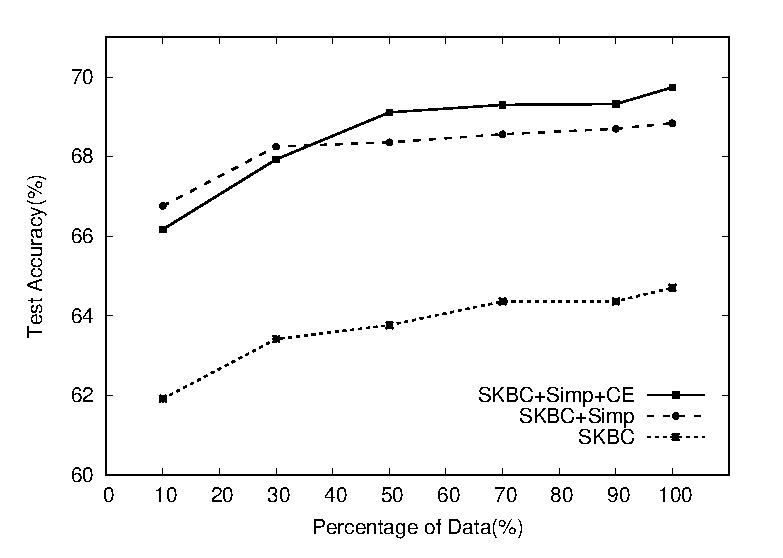
\includegraphics[width=0.8\columnwidth]{figures/story/trend}
\caption{不同训练数据规模下的准确率。}\label{fig2:trend}
\end{figure}

\figref{fig2:trend} 对比了在增加的训练数
据量(ROCS*(Tr))下,不同方法的模型性能。首先可以
看到,我们的两种方法(Simp和Simp+CE)即使在较少的训练数据下也
能表现出色。事实上,仅使用10\%的数据,它们就已经
超过了SKBC在全部数据下的准确率。其次,我们观察到与SKBC相
比,采用我们方法的模型在训练数据增加时提升更快,这一点从10\%到50\%数据量的斜率中尤为明显。
最后,比较有无概念嵌入的效果,我们发现,在没有结构化知识支持的情况下,模型难以利用更多训练数据。

\subsubsection*{5. 训练时间}
\label{sec2:time}
除了端到端准确率的提升外,简化后的概念序列编码方法还能将训练时间缩短至原来的三分
之一。这种效率提升得益于句子中词汇数量的减少和词汇表的缩小。ROC故事
中共有43,095个独特词汇,而从ConceptNet中提取的简化关键词汇仅有19,455个,这
大大减少了词汇表的大小。



\subsection{本章小结}

在本章中,我们专注于解决人工智能模型在理解和预测故事结局的任务中面临的一个核心挑战:
如何提升模型的常识性推理能力。考虑到故事理解涉及广泛而复杂的常识知识,
我们选择了故事结局预测这一特别具有挑战性的任务作为我们研究的焦点。
为此,我们提出了一种新颖的方法论,旨在通过精确识别和分析故事中的关键常识概念和事件,
从而使模型能够更深入地沿故事线索进行推理。这种方法的创新之处在于,
它不仅关注故事的表意,而且深入挖掘故事结构中的隐含逻辑和关系。

我们的方法包括三个关键部分:首先是对故事句子的简化处理,以突
出关键概念和事件;其次是基于这些关键元素构建更加丰富和细致的故事表
示;最后是运用这种表示来预测故事结局。为了实现这一目标,我们结合了句子
的概念序列编码和ConceptNet预训练的概念图编码,这一步骤对于捕捉故
事中的深层关系至关重要。

在实验部分,我们使用了一个经过精心设计的数据集,旨在减少偏见和提
高预测的准确性。我们的模型与多种现有的基线模型(如DSSM、SKBC和BERT)进
行了对比。实验结果表明,我们的方法在减少训练数据中的偏见和信息泄露方面表现
优异。此外,我们还探讨了不同的简化策略和概念嵌入的影响,
发现结合ConceptNet的预训练概念嵌入能够显著提升模型性能。

最后,本章提出了未来研究方向,主要聚焦于如何显式表示故事中的常识关系,
以提升模型对预测结果的解释能力。这种方法的发展不仅能增强模型的透明度,
还能为未来的研究提供关于故事理解和推理机制的更深刻见解。







\newpage
\fancyhead[LH]{上海交通大学学位论文}
\fancyhead[RH]{第四章\quad 推理模型鲁棒性不足的可解释性分析}
\setcounter{figure}{0}
\setcounter{table}{0}
\section{推理模型鲁棒性不足的可解释性分析}
%\section{常识性推理任务中的偏差识别与评估架构}



%在本章节的开篇,我们将聚焦人工智能领域的一个关键挑战:解析推理模型鲁棒性差的原因。
%如\secref{sec1:interpretability}所述,我们认识到,尽管利用如
%CheckList工具的现有评估方法为理解模型的鲁棒性提供了关键洞见,但这些方法在揭
%示模型确切学习内容及其背后的复杂动态方面显得力不从心。这突显出一个研究空白:目
%前对模型所学内容及其背后的复杂机制的理解,仍然缺乏系统性和深度。
%
%应对这一挑战,我们可以从两个角度出发:数据的角度或者模型的角度。因为最终应用的模型
%实体是数据和模型结构共同作用的结果。在本节的研究中,我们主要从\textbf{数据的角度}进行分析解释。

在\secref{sec1:interpretability}中,我们深入探讨了模型在处理常
识性推理任务时表现的鲁棒性不足的现象以及这个现象的可解释性上。
虽然这些模型在标准测试环境下展现出色,但它们在面对对抗性数据或
与训练环境截然不同的情形时,却展现出显著的脆弱性。众多研究提出了一个
关键假设,即这种鲁棒性不足可能源自模型对数据中特定结构元素的过度依赖,
如偏见线索或虚假线索。这一假设背后的深层次原因在于数据集的构建方式,
这导致模型倾向于学习数据特有的简化规则而非广泛适用的解决策略。

为了对这一假设进行验证,研究者们引入了``仅假设''测试和注意力图等工具。
这些方法使研究者能够更深入地分析模型可能对数据中某些特定结构元素的过分关注。
然而,这些方法在解释模型行为方面存在一定的局限性。例如,``仅假设''测试并不能
充分展现模型在处理真实场景时的推理模式,因为它的测试数据结构与模型在训练阶
段所接触的数据结构并不一致。同样,尽管注意力图被用来揭示模型的焦点,但相关
研究表明,模型通过注意力机制突出显示的内容并不总是准确反映其决策的真实依据。
鉴于此,深入探索
数据偏见如何具体作用于模型的机制已成为一个迫切且重要的研究课题。

我们将在本章介绍两种创新的测试框架,用以深入分析并理解数据偏见对模型鲁棒性的影响。
首先,我们提出的宏观层面测试框架,通过将测试数据划分为简单(easy)和困难(hard)两类,
对模型在识别和处理虚假特征方面的能力进行量化评估。此方法揭露了模型对特定统计规
律的过度依赖,帮助我们深入理解模型泛化能力的局限。

其次,我们引入了微观统计分析框架——ICQ(``I-see-cue'')框架,它通过多维特
征划分和细致的性能分析,探究模型在不同特征上的准确性和分布表现。此外,我们还
开发了一种直观的可视化工具,旨在更有效地识别和理解模型性能差异的根源。

总体而言,本研究的主要贡献在于这两种高度创新的分析框架,它们为深入解析常识性推理模型的鲁棒性不足问题
提供了新的路径。
%通过结合宏观与微观方法,我们能够全面
%评估模型在处理复杂数据时的行为模式,尤其是在识别和处理潜在虚假特征方面的能力。这些成
%果不仅揭示了模型的潜在薄弱环节,也为未来设计更加健壮且可解释的人工智能系统打下了坚实的基础。

\subsection{概述}
\label{sec4:intro}
深度神经网络模型在各种自然语言理解(NLU)任
务中取得了显著的成就,这些任务包括自然语言
推理~\cite{bowman2015large,wang2018glue}、论证分析~\cite{niven2019probing}、常
识推理~\cite{mostafazadeh2016corpus,roemmele2011choice,zellers2018swag}、阅读理
解~\cite{lai2017race}、问题回答~\cite{talmor2019commonsenseqa}和对话
分析~\cite{lowe2015ubuntu}。这些任务经常采用多项选择框架,正如在斯坦福
自然语言推理(SNLI)数据集的例子中所示(见 \exref{exp4:snli})。然而,近期研究~\cite{gururangan2018annotation,sanchez2018behavior,poliak2018hypothesis,checklist2020acl}揭示了
一些问题,特别是在这些模型对微小变化高度敏感的背景下,我们需要一个更为稳健且精确的评估机制。

\begin{center}
    \begin{example}\label{exp4:snli}
    SNLI 数据集中的自然语言推理示例,正确答案以斜体标出
    \begin{description}
    \item{Premise:} A swimmer playing in the surf watches a low flying airplane headed inland.
    \item{Hypothesis:} Someone is swimming in the sea.
    \item{Label:} \textit{a) Entailment.} b) Contradiction. c) Neutral.
    \end{description}
    \end{example}
    \end{center}
在处理类似 \exref{exp4:snli} 这样的任务时,人类通常依赖于前提和假设之
间的逻辑关系。与此相反,一些 NLP 模型可能会绕过这种逻辑推理,转而关注数据集
中嵌入的偏见,特别是在假设中的偏见~\cite{naik2018stress,schuster2019towards}。
这些偏见,如情感或表层 n-grams,可能为正确预测提供误导性线索。

当这些偏见在训练和测试数据集中普遍存在,并在预测上保持类似的分布时,我们将其
称为``人为虚假线索''(如图 \ref{fig4:cue_def} 所示)。例如,在 \exref{exp4:snli} 中,某
些模型可能过分依赖``someone''一词来做出判断。这种情况下,当这些线索缺失或改变时,可能会显
著影响模型的性能,凸显了识别这些线索以提高模型鲁棒性的重要性。

\begin{figure}[th]
\centering
\includegraphics[width=0.50\columnwidth]{figures/emnlp/cue_def.eps}
\caption{线索的示例。}
\label{fig4:cue_def}
\end{figure}


本研究旨在探讨如何在各类自然语言理解任务中识别和解决虚假线索的问题。
我们特别关注这些线索在数据集制作过程中如何产生,以及模型在训练过程
中如何学习并依赖这些线索。我们提出的方法旨在揭示这些线索,并帮助我们
深入理解它们如何影响模型的性能和推理能力。为此,我们将从宏观和微观两
个角度分析模型是否受到虚假线索的影响。

\subsubsection*{宏观角度分析}
我们提出了一种新方法,用以从宏观角度分析自然语言理解(NLU)任务中虚假线索的问题。
在探索人类处理这类问题的方式时,我们发现人们通常会仔细分析问题的前提和假设之间的
逻辑关系。然而,之前的研究~\cite{naik2018stress,schuster2019towards}显示,
许多自然语言处理(NLP)模型在处理类似问题时,往往只考虑假设部分,忽视了逻辑关系
的深入分析。这一现象在很大程度上归咎于数据集中人工制作的假设存在的瑕疵。

虽然``仅假设''测试在理论上是用于识别此类问题的有效方法,但它常依赖于特定
的、如BERT~\cite{devlin2018bert}这样的模型,这就需要进行模型的重新训练。
更重要的是,``仅假设''测试并不能
充分展现模型在处理真实场景时的推理模式,因为它的测试数据结构与模型在训练阶
段所接触的数据结构并不一致。

在我们的研究中,我们开发了一种轻量级框架,专注于识别多项选择自然语言
推理数据集中的关键且影响力显著的线索。尽管不是所有多项选择题都包含前
提、假设和标签,但我们在第 \ref{sec4:approach1} 节中详细介绍了如何将
这些元素标准化。我们的框架以词汇为基础,利用它们作为构建线索的关键特征,因
为词汇在大多数现代机器学习方法中是自然语言建模的基石。此外,即便是复杂的语
言特征,如情感、风格和观点,也通常是基于词汇特征。

我们的实验展示了,基于词汇的线索在检测数据集中的统计偏差方面,与资源消
耗更大的``仅假设''方法同样有效。这一发现对于理解和改进模型的推理能力至关重要。

此外,我们还设计了一种方法,将测试数据基于问题是否能仅通过线索特征被
正确回答的能力,划分为简单和困难两个子集。数据集中困难部分的相对大小是衡
量其整体质量的重要指标,其中困难部分占比越大,表明数据集质量越高。这种划分
同时也是一种``压力测试'',可用于评估模型的真实推理能力。两个子集间的分类准确
率差异揭示了模型在不同情境下的潜在薄弱环节。

%最后,我们还提出了一种划分训练数据的简单方法,将其分为简单和困难两部分。这样做的目的是,通过让模型专注于更复杂的线索,从而提高其在处理困难问题时的推理能力。

综上所述,这个宏观层面的方法的研究贡献有两个。首先,我们开发了一种轻量级但有效的方法,用
于评估和识别自然语言理解数据集中的统计偏见和虚假线
索(\secref{sec4:approach1}、\secref{sec4:experiment1} )。
另外,我们通过将测试数据划分为简单和困难两部分,根据信息泄露程度来
评估模型的真实推理能力,从而量化比较这两部分的性能差异(\secref{sec4:experiment1} )。

\subsubsection*{微观角度分析}
在微观层面上,我们的研究着重于区分数据集中预先嵌入的
线索与模型在训练过程中所学习的线索。传统的偏见检测与缓解工具,
如 AI Fairness 360 工具包~\cite{bellamy2018ai},尽管主要聚焦
于数据集中的偏见,但在处理模型训练过程中产生的偏见时,它们往往显示出局限性。

现有的方法,例如``仅假设''测试和 CheckList,虽然能够揭示模型的脆
弱性,却不是专门为识别模型学习的线索而设计的。具体来说,``仅假设''测试能
够突显出数据集中的某些问题,如仅凭假设就能得出正确答案的情况,但这并未涵盖
模型在训练和预测过程中使用的完整数据上下文,因此无法全面反映模型的整体能力。

同样地,虽然 CheckList 采用了软件工程中的黑盒测试原则,通过对预
定义语言特征的额外压力测试案例来审视模型的弱点,但它对精心设计的模板的
依赖限制了其应用范围。这种方法能够揭示模型的脆弱性,
%类似于我们在上一章
%节构造的代理测试(参见\secref{sec3:approach} 节),
但它并不能清楚地揭
示模型实际从数据中学到的具体知识或特征。

尽管我们的宏观架构能够在一定程度上分析模型受到数据中虚假线索的影响程度,
但它难以具体指出受到哪些特定线索的影响。

为了克服这些局限,我们引入了 ICQ(``I-see-cue'',意为``我发现线索''),
一个灵活的统计分析框架\footnote{代码和数据集可在 \url{https://github.com/flora336/icq} 获取}。
ICQ 的设计哲学与传统方法完全不同,它能够在不需要额外测试案例的情况下,有效识别多项选择
 NLU 数据集中的偏见。采用黑盒测试方法,ICQ 能够评估模型如何利用这些偏见,从而为理解
  NLU 任务中的偏见提供全面且深入的见解。

我们通过在不同的 NLU 数据集上部署 ICQ 来验证其有效性,并探索模型在训练
期间可能学习到的线索。ICQ 的应用极大地促进了我们对于诸如 ChatGPT%\footnote{\url{https://chat.openai.com/}}
这类模型如何学习潜在
线索的深入理解,并提供了选择合适提示的示例,为模型的优化提供了重要的指导。

综上所述,我们的微观研究主要提供了以下几点贡献:
\begin{itemize}
\item 我们推出了 ICQ,这是一种轻量级且功能强大的工具,专门用于识别 
NLU 数据集中的统计偏见和线索。我们还提出了简单而有效的测试方法,以量化和
直观地评估模型是否在其预测中利用了虚假线索。
\item 我们对十个流行的 NLU 数据集和四个模型进行了全面的统计偏见问题
评估,从而证实了先前的发现并揭示了新的见解。我们还提供了一个在线演示系
统,展示结果并邀请用户评估他们自己的数据集和模型。
\item 通过一个案例研究,我们深入探讨了 ChatGPT 如何学习潜在偏见,并为
其实际应用提供了宝贵的建议。
\end{itemize}

\subsection{相关工作}
\label{sec3:related}

我们的工作涉及三个研究方向:虚假特征分析、偏见计算和数据集过滤。

\subsubsection*{虚假特征分析}
近年来,虚假特征分析在自然语言处理(NLP)领域获得了越来越多的关注。研究表明,许多 NLP 模型能够在多项选择题形式的自然语言理解问题中取得良好表现,有时甚至无需深入理解问题的核心内容。这类现象在某些研究中被称为``仅假设''测试~\cite{sharma2018tackling,srinivasan2018simple,zellers2018swag}。此外,研究发现,这些模型对于假设中的微小但语义重大的变化并不敏感,推测这种``仅假设''表现可能源于假设中的词语与答案标签之间的简单统计关联~\cite{sanchez2018behavior}。

虚假特征可分为词汇化和非词汇化两类~\cite{bowman2015large}。词汇化特征主要包括 n-gram 词标和交叉 n-gram 词标,而非词汇化特征则涉及词汇重叠、句子长度以及前提和假设之间的 BLEU 分数。词汇化分类的细化,如否定、数值推理和拼写错误,也在文献中得到了探讨~\cite{naik2018stress}。另一方面,非词汇化特征如词汇重叠、子序列和成分被进一步细化,同时也考虑了句法结构重叠~\cite{mccoy2019right}。此外,\cite{sanchez2018behavior}为未见过的词汇标记提供了额外的词汇化特征。

\subsubsection*{偏见计算}
偏见计算关注于量化线索的严重性。一些研究尝试通过仅假设训练或从嵌入中提取与特定标签相关的特征来隐式编码线索特征~\cite{clark2019don,he2019unlearn,yaghoobzadeh2019robust}。其他方法则采用统计指标来计算偏见。例如,\cite{yu2020reclor}使用在特定标签下观察到某个词的概率来对词进行偏见排名。LMI(局部互信息)被用于评估线索并在某些模型中进行重权~\cite{schuster2019towards}。然而,这些研究并没有充分解释为什么选择这些指标而非其他指标。此外,\cite{Marco2020acl}提供了一种测试数据增强方法,但它没有评估偏见的程度。

\subsubsection*{数据集过滤}
数据集过滤是一种通过减少数据集中人为制作特征来提高数据集质量的方法。
事实上,本研究评估的 SWAG 和 RECLOR 等数据集就是采用这种过滤方法的变体生成的。这种方法通过反复扰动数据实例,直到目标模型无法再很好地拟合所得数据集为止。一些方法不是通过预处理数据来去除偏见,而是在训练过程中根据每个阶段的决策排除带有偏见的样本~\cite{yaghoobzadeh2019robust}。\cite{bras2020adversarial}探讨了基于模型的数据集线索减少算法,并设计了一种使用迭代训练的算法。这种方法比人工标注更通用、更高效,但它严重依赖于所使用的模型。不幸的是,不同模型可能会捕捉到不同的线索,因此这些方法可能并不完全。

本节涉及的三个主要研究方向对于当前人工智能领域至关重要。虚假特征分析揭示了模型可能依赖的非理想特征,偏见计算提供了量化这些特征的方法,而数据集过滤旨在减少数据集中的人为制作特征,以提高其整体质量。这些研究方向为理解和改善 NLP 模型在处理自然语言任务时的表现提供了重要的视角和工具。

\subsection{任务表述}

在本节中,我们将介绍如何将自然语言推理任务的数据集 $X$ 中的问题实例 $x$ 进行标准化表述。对于数据集 $X$ 中的每个问题实例 $x$,我们定义其为以下形式:
\begin{equation}
x = (p, h, l) \in X,
\end{equation}
\noindent
其中 $p$ 代表推理的上下文,即给定的情景或陈述,类似
于例子~\ref{exp4:snli}中的``前提'';$h$ 是针对上下文 $p$ 的假设
或断言;$l \in \mathcal{L}$ 是一个标签,用于描述上下文 $p$ 和假设 $h$ 之间的关系类型。

在不同的自然语言推理任务中,关系集合 $\mathcal{L}$ 的大小可能会有
所不同。通常,这种关系集合能够涵盖任务所需表达的所有可能关系类型。例
如,在一个典型的自然语言推理问题中,包含一个\textit{前提}($p$)、一
个\textit{假设}($h$)和一个描述前提与假设之间关系的\textit{标签}($l$)。对
于描述\textit{蕴涵}、\textit{矛盾}和\textit{中立}三种不同关系的场景,关系集
合 $\mathcal{L}$ 的大小为 $|\mathcal{L}| = 3$。

我们认为,这种通用形式能够适用于大多数具有区分性的自然语言推理任
务。在第~\ref{sec4:dynamic}节中,我们将进一步讨论如何将不同类型的自然语言推理任务
转换为这种标准化表述,以便于进行更系统和统一的分析。这种标准化的方法不仅有助于
简化任务的理解和实现,还为后续的模型训练和评估提供了清晰的指导。

%在本节中,我们将深入探讨两种架构,用于识别和评估数据集及其模型中的偏差:
%一种是宏观架构,另一种是微观架构。我们会详细说明这些架构如何揭示数据和模型学习中的偏差信息。
\subsection{宏观偏差识别与评估架构}
\label{sec4:approach1}
在宏观架构中,我们专注于使用统计特征来评估数据集内的偏差。首先,我们
对自然语言推理任务进行通用化的表述。随后,通过计算与每个标签关
联的词汇频率,我们设计了衡量词汇和标签相关性的指标,称之为``线索分数''。这些
分数揭示了潜在的偏差模式。我们进一步利用简单的统计模型来汇总这些分数,并据此作出
预测。最后,我们展示了如何利用这些快速预测方法,将数据集划分为``简单''和``困难''两部分。

\subsubsection{线索度量}

对于给定的数据集\(X\),我们收集其中所有词汇的集合\(\mathcal{N}\)。线索度量是衡量
特定词在不同标签下出现频率的不平衡性。对于集合中的词\(w\),我们用以下八种方法中的一
种来计算其线索分数\(f_{\mathcal{F}}^{(w,l)}\)。我们将这些度量分为两大类:前四
种基于简单统计数据,后四种则涉及欧几里得空间中的角度概念。

设\(\mathcal{L'} = \mathcal{L} \setminus \{l\}\),我们定义
\begin{equation}
\#(w, \mathcal{L'}) = \sum_{l' \in \mathcal{L'}} \#(w, l').
\end{equation}

\textbf{频率(Freq)}
最基础的度量是词汇和标签的共现频率,其中\(\#()\)\ 表示简单计数。这个度量
旨在捕捉词汇在特定标签下的原始频率:
\begin{equation}
f_{Freq}^{(w,l)} = \#(w, l).
\end{equation}

\textbf{相对频率(RF)}
相对频率在频率的基础上进行扩展,考虑了词汇在所有标签下的总频率。公式如下:
\begin{equation}
f_{RF}^{(w,l)} = \frac{\#(w, l)}{\#(w)}.
\end{equation}

\textbf{条件概率(CP)}
标签\(l\)在词\(w\)下的条件概率是另一种重要的度量,用于捕捉特定条件下的概率分布:
\begin{equation}
f_{CP}^{(w,l)} = p(l|w) = \frac{\#(w, l)}{\#(w)}.
\end{equation}

\textbf{点互信息(PMI)}
点互信息是信息论中用于衡量词汇和标签关联强度的常用指标。当词汇和标签共现的频率超出独立出现的预期频率时,PMI值较高。其定义如下,其中\(p(w)\)和\(p(l)\)分别是\(w\)和\(l\)的概率,\(p(w,l)\)是它们的联合概率:
\begin{equation}
f_{PMI}^{(w,l)} = \log \frac{p(w,l)}{p(w)p(l)}.
\end{equation}

\textbf{局部互信息(LMI)}
局部互信息是PMI的变体,它通过词汇和标签的联合概率加权PMI,给予频繁出现的词汇-标签对更多重视:
\begin{equation}
f_{LMI}^{(w,l)} = p(w, l)\log \frac{p(w,l)}{p(w)p(l)}.
\end{equation}

\textbf{比率差异(RD)}
比率差异衡量词汇-标签比率与整体标签比率之间的绝对差异,有助于识别特定标签不成比例相关的词汇:
\begin{equation}
f_{RD}^{(w,l)} = \left|\frac{\#(w, l)}{\#(w, \mathcal{L'})} - \frac{\#(l)}{\#(\mathcal{L'})}\right|.
\end{equation}

\textbf{角度差异(AD)}
角度差异类似于比率差异,但通过使用反正切函数,考虑了比率之间的非线性关系,
使度量对异常值更加稳健:
\begin{equation}
f_{AD}^{(w,l)} = \left| \arctan\frac{\#(w, l)}{\#(w, \mathcal{L'})} - \arctan \frac{\#(l)}{\#(\mathcal{L'})} \right|.
\end{equation}

\textbf{余弦(Cos)}
余弦度量将\(v_w=[\#(w, l), \#(w, \mathcal{L'})]\)和\(v_l = [(\#(l), \#(\mathcal{L'})]\)视为二维空间中的两个向量。
如果\(v_w\)和\(v_l\)共线,则意味着\(w\)没有提供误导性信息。
否则,\(w\)可能是虚假线索,因为它倾向于与某个特定标签\(l\)更频繁共现。
这个度量通过几何方式量化了词汇-标签关系的相似性:
\begin{equation}
f_{Cos}^{(w,l)} = \cos(v_w, v_l).
\end{equation}

\textbf{加权功率(WP)}
加权功率结合了余弦度量和基于频率的加权,强调了高频词汇的重要性,帮助
优先考虑对模型影响更大的线索:
\begin{equation}
f_{WP}^{(w,l)} = (1-f_{Cos}^{l})\#(w)^{f_{Cos}^{l}}.
\end{equation}

总结来说,我们可以将词\(w\)相对于标签\(l\)的线索分数表示
为\(f^{(w,l)}\),省略方法下标\(\mathcal{F}\)。这些度量从多个角
度提供了关于词汇和标签之间关联性的洞见,有助于识别潜在的虚假相关性。

\subsubsection{聚合方法}

我们可以使用简单的方法 \(\mathcal{G}\) 来聚合问题实例 \(x\) 中的词语线索分数以作出预测。这些方法旨在易于实现和计算效率高,鉴于线索特征的低维性。

\textbf{平均值和最大值}

预测标签最直接的方法是选择具有最高平均或最大\textit{线索分数}的标签。

\begin{equation}
    \mathcal{G}_{\text{average}} = \mathop{\arg\max}_{l} \left(\frac{\sum_{w}f^{w,l}}{|x|}\right), \quad l \in \mathcal{L}, w \in \mathcal{N}
\end{equation}

\begin{equation}
    \mathcal{G}_{\text{max}} = \mathop{\arg\max}_{l} \left(\max_w(f^{w,l})\right),
    \quad l \in \mathcal{L}, w \in \mathcal{N}
\end{equation}

\textbf{线性模型}

为了更好地利用\textit{线索分数}进行预测,我们采用了两种简单的线性模型:SGDClassifier和逻辑回归。模型的输入是问题实例 \(x\) 中每个标签的\textit{线索分数}的连接向量:
\begin{equation}
\text{input}(x) = [ f^{(w_1, l_1)}, \ldots, f^{(w_d, l_1)}, f^{(w_1, l_2)}, \ldots, f^{(w_d,l_2)}, \ldots, f^{(w_1,l_t)}, \ldots, f^{(w_d,l_t)}]
\end{equation}
在实际应用中,输入向量被填充到相同长度。线性模型的训练损失为:

\begin{equation}
    \hat{\phi}_n = \mathop{\arg\min}_{\phi_n} \left(\text{loss}\left(\mathcal{G}_{\text{linear}}(\text{input}(x); \phi_n)\right)\right)
\end{equation}

损失是根据黄金标签 \(l_g\) 和预测标签 \(\mathcal{G}_{\text{linear}}(\text{input}(x); \phi_n)\) 计算的。 \(\phi_n\) 表示在 \(\mathcal{G}_{\text{linear}}\) 中最小化 \(l_g\) 的损失的最优参数。

\subsubsection{多项选择题的标准化转换}
\label{sec4:dynamic}

到目前为止,我们关注的是具有固定选项集的多项选择题(MCQs)。
然而,一些语言推理任务涉及到具有非固定选项的MCQs,如ROC数据集。在这些情况下,
我们可以将原始故事分为两个统一实例,\(u_1=(\text{context}, \text{ending1}, \text{false})\) 和 \(u_2=(\text{context}, \text{ending2}, \text{true})\)。
我们预测每个实例的标签概率,\(\mathcal{G}(\text{input}(u_1); \phi)\) 和 \(\mathcal{G}(\text{input}(u_2); \phi)\),并选择具有更高概率的结局作为预测。


\subsubsection{数据集难度层级分类方法}
本小节旨在介绍一种区分数据集中问题难度的方法,通过预测结果将问题分类为简单或困难。这种分类依赖于一个聚合模型,其核心在于利用词频特征进行有效预测。该方法不仅有助于评估模型在处理各种难度问题时的性能,而且能够揭示数据集中的潜在信息泄露。

具体来说,我们对数据集中的每个问题进行预测。如果问题被模型正确预测,我们则将其标记为``简单'';
如果预测失败,则标记为``困难''。通过这一流程,我们可以将整个数据集有效地分为两个子集,
即简单问题集和困难问题集,进而更深入地理解模型的性能及其在不同情境下的应用潜力。
我们可以按照以下步骤将数据集分为简单和困难的问题,参见算法\ref{alg4:easyhard}:
\begin{algorithm}[H]
    \caption{将数据集分为简单和困难部分}
    \label{alg4:easyhard}
    \begin{algorithmic}[1]
    \Require dataset $\mathcal{D}$, aggregation model $\mathcal{G}$, number of folds $n$, number of iterations $k$
    \State Initialize a counter $C$ for each question $q$ in $\mathcal{D}$ as 0
    \For{$i = 1$ to $k$}
    \State Perform $n$-fold random split of $\mathcal{D}$ into ${P_1, P_2, \dots, P_n}$
    \For{$j = 1$ to $n$}
    \State Train $\mathcal{G}$ on ${P_1, P_2, \dots, P_{j-1}, P_{j+1}, \dots, P_n}$
    \State Test $\mathcal{G}$ on $P_j$
    \For{each question $q$ in $P_j$}
    \If{$q$ is correctly predicted}
    \State Increment $C[q]$
    \EndIf
    \EndFor
    \EndFor
    \EndFor
    \State Label each question $q$ in $\mathcal{D}$ as easy if $C[q] > \frac{k}{2}$, otherwise label as hard
    \State Split $\mathcal{D}$ into easy and hard parts based on the labels
    \end{algorithmic}
    \end{algorithm}
具体来说分成以下六个步骤:
\begin{enumerate}
\item 对数据进行 \(n\) 折随机划分。
\item 在 \(n-1\) 部分上训练聚合模型。
\item 采用循环赛方式,在剩余的部分上测试聚合模型。
\item 每个问题测试一次后,根据模型的预测结果为其分配``简单''或``困难''标签。
\item 重复此过程多次(例如 \(k\) 次迭代),并根据 \(k\) 次迭代中的多数标签为每个问题标记。
\item 最后,根据每个问题的最终标签,将数据集分为简单和困难两部分。
\end{enumerate}
此算法使我们能够更好地理解模型在不同难度级别上的表现,并仅使用统计特征分析数据集的信息泄露。通过测量词语和标签之间的相关性,
聚合线索分数以进行预测,并根据难度将数据集进行分割,我们可以评估模型的真实推理能力,
并解决由虚假线索引起的潜在问题。这个过程旨在计算效率高、易于实现,适用于广泛的自
然语言推理任务。

\subsection{微观偏差识别与评估架构}
\label{sec4:approach2}
在微观层面上,偏差识别和评估涉及对数据集的深入分析,
以发现和评估潜在的偏见和不平衡。这种分析要求我们关注数据的具体细节,
如语言特征和模型对这些特征的响应。本节首先介绍了作为分析基础的关键语言特征,
然后描述了我们的ICQ框架,它是对这些特征进行系统化检查和评估的工具。
\subsubsection{相关语言特征}
\label{sec4:extract}
在微观偏差分析的第一步中,我们关注数据集中的特定语言特征,
这些特征可能揭示或促成了偏见的形成。如先前的研
究~\cite{naik2018stress,checklist2020acl}所示,我们考虑以下关键语言特征:

\indent\textbf{词汇}:数据集实例中前提或假设中特定词汇的存在。

\indent\textbf{情感}:实例的情感值,计算为单个词语情感极性的总和。

\indent\textbf{时态}:实例的时态特征(过去、现在或未来),由根动词的词性标记决定。

\indent\textbf{否定}:实例中负面词汇(例如``no''、``not''或``never'')的存在,通过依存解析确定。

\indent\textbf{重叠}:至少有一个词(排除停用词)同时出现在前提和假设中。

\indent\textbf{命名实体识别(NER)}:实例中命名实体(例如PER、ORG、LOC、TIME或CARDINAL)的存在,使用NLTK NER工具检测。

\indent\textbf{拼写错误}:实例中至少存在一个拼写错误,使用预训练的拼写模型识别。

对于多项选择数据集,除了重叠外的所有特征仅应用于假设。

\subsubsection{ICQ框架}
在确定了关键的语言特征后,我们引入ICQ框架(如~\figref{fig4:framework}所示),
它是一个三阶段的过程,包括数据提取、线索发现和模型探测。ICQ框架专注于系统地分析这些语言特征,
以揭示潜在的偏差和不一致。

\textbf{数据提取阶段(Data Extraction)}:在这一阶段,我们从数据集中提取包含特定语言特征$f$的实例。
这一步骤是识别潜在偏见的基础。

\textbf{线索发现阶段(Cue Discovery)}:紧接着,我们对提取出的实例进行深入分析,以识别其中的潜在线索。
这涉及到对每个预定义特征的详细检查。

\textbf{模型评估阶段 (Model Probing)}:最后,我们进行两项测试:``准确性测试''(Accuracy Test)和``分布测试''(Distribution Test)。
这些测试旨在评估模型对不同特征的反应,以及这些反应是否揭示了模型的任何偏见或不平衡

%如~\figref{fig4:framework}所示,ICQ框架包括三个阶段:数据提取、线索发现和模型探测。
%在数据提取阶段,从数据集中提取包含特定语言特征$f$的实例。线索发现阶段识别预定义特征中的潜在线索。
%最后,模型探测阶段进行两项测试:``准确性测试''和``分布测试''。我们将在下面更详细地讨论这些阶段。

\begin{figure}[th]
\centering
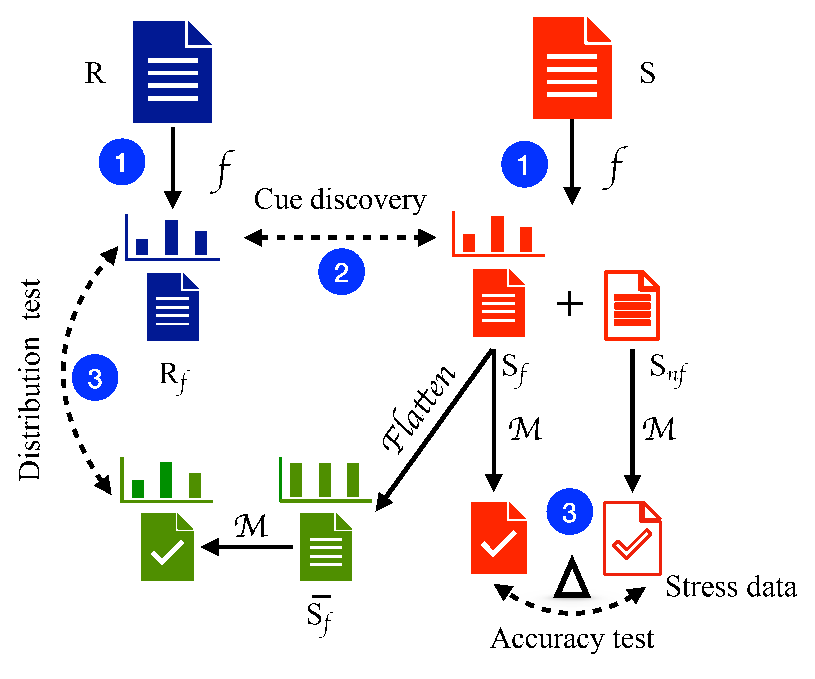
\includegraphics[width=0.8\columnwidth]{figures/emnlp/framework.eps}
\caption{ICQ工作流程。 \textcircled{1}:数据提取阶段; \textcircled{2}:线索发现阶段;
\textcircled{3}:模型探测阶段。$f$=特定特征,$R$=训练数据,$S$=测试数据,$R_f$=提取的训练数据,
$S_f$=提取的测试数据,$S_{nf}$=不包含特征$f$的剩余测试数据,$\overline{S_f}$=平衡化测试数据(flatten),$\mathcal{M}$=特定模型。}
\label{fig4:framework}
\end{figure}

我们将在下面更详细地讨论这些阶段:
\subsubsection*{1. 数据提取阶段}
\label{sec4:evaldata}
在确定了关键的语言特征之后,我们的系统首先执行的任务是构建数据提取器。对于每个特征值 \(f\),提取器的角色是处理整个数据集并识别与该特定特征值相关联的实例。具体来说,如果数据集中的某个实例包含了这个特征,那么这个实例就会被选中,并归入包含该特征的子集中。这一步是识别特征在数据集中分布和表现的基础。

\subsubsection*{2. 线索发现阶段}
\label{sec4:cuenessdiscovery}

接下来,我们针对每个特征 \(f\),将其对应的提取器应用于数据集 \(X\) 的训练和测试部分,分别标记为 \(R\) 和 \(S\),如图 \ref{fig4:framework} 所示。这导致了基于特征的实例聚类,形成了训练实例子集 \(R_f\) 和测试实例子集 \(S_f\)。一个特征被视为潜在的数据集线索,当且仅当它同时存在于训练和测试数据中。

为了计算提取集的标签分布偏差,我们使用均方误差(MSE)和Jensen-Shannon Divergence(JSD)~\cite{lin1991divergence}。线索得分反映了数据集 \(X\) 针对特征 \(f\) 的偏见程度。

均方误差(MSE)计算方法如下:
\begin{equation}
MSE(F) = \frac{1}{|\mathcal{L}|} \sum_i (y_i - \overline{y_i})^2
\end{equation}
其中,\(y_i\) 表示在提取数据集 \(F\) 中标签 \(l_i\) 的实例数,而 \(\overline{y_i}\) 是每个标签的平均实例数。较大的 \(MSE(F)\) 意味着更尖锐的标签分布,指示了更显著的偏见。

如果提取的训练集 \(R_f\) 和提取的测试集 \(S_f\) 展示出类似的偏见,那么它们分布之间的JSD将会很小。JSD的计算公式为:
\begin{equation}
JSD = \frac{1}{2}\left (Q(R_f) \parallel A \right ) + \frac{1}{2}\left (Q(S_f) \parallel A \right ),
\end{equation}
其中 \(A = \frac{1}{2}\left (Q(R_f) + Q(S_f) \right )\)。函数 \(Q()\) 表示提取数据集的标签分布。

最后,我们定义线索得分,用以衡量数据集 \(X\) 针对特征 \(f\) 的偏见程度:
\begin{equation}
cue(f, X) = \frac{MSE(R_f)}{\exp(JSD(R_f, S_f))}
\end{equation}
这个得分结合了标签分布的不均衡(MSE)和在训练与测试集之间分布的一致性(JSD),从而提供了一个全面的偏见指标。

\subsubsection*{3. 模型测试阶段 (Model Probing)}
\label{sec4:modelprobing}
在前两个结算,我们探讨了数据集 \(X\) 可能受特定线索 \(f\) 影响的可能性。
然而,关键的问题在于,基于这个数据集训练出的模型是否真的会利用这一线索。这不仅
与数据集的特性有关,而且还取决于模型的结构和训练机制。为了深入探索这一点,在第三阶段介绍
了一套框架,用于探测和评估在有偏数据集上训练的模型是否以及在多大程度上利用了特定线
索 \(f\)。此框架包括两种测试方法:准确性测试和分布测试。

\subsubsection*{准确性测试}
\label{sec4:accuracytest}
准确性测试旨在评估模型在含有和不含有特定特征 \(f\) 的数据子集上的表现差异。
这种比较能够揭示模型在面对不同数据情景时的泛化能力。具体来说,如果模型在包含特
定特征 \(f\) 的数据子集上表现更佳,这通常意味着模型已经学会利用这一特征进行预测。

在准确性测试中,我们专注于测量模型 \(M\) 在两个测试集上
的表现:一个是包含特征 \(f\) 的测试集 \(S_f\),另一个是不包含特征 \(f\) 的测
试集 \(S_{nf}\)。我们通过以下公式计算这两个测试集上准确率的差异:

\begin{equation}
\Delta Acc(f) = acc(S_f) - acc(S_{nf})
\end{equation}

这里的 \(\Delta Acc\) 值揭示了模型在处理包含和不包含特定
特征的数据子集时性能的变化。$\Delta Acc$的正值或负值表明模型在比较包含
和不包含特定特征的数据子集时性能变化的方向。正值表明模型利用该特征进行预测,
而负值则意味着模型在泛化或对该特征的敏感性上存在困难。
$\Delta Acc$的绝对值大小反映了模型性能受到特定特征存在或缺失的影响程度。
较大的绝对值表明模型更依赖或对该特征更敏感,而较小的绝对值则表明模型更健壮,
对特征的存在或缺失影响较小。


\subsubsection*{分布测试 (Distribution Test)}
\label{sec4:distributiontest}
分布测试着重于通过视觉化的方式检查特定特征的分布变化如何影响模型的预测性能。
这一测试的第一步是在提取的测试集 \(S_f\) 中创建
一个``平衡化''测试集 \(\overline{S_f}\)。我们通过平
衡化标签分布来实现这一点,即从每个标签类别中随机移除实例,直到所有
类别的实例数量相等。这一过程主要包括以下几个步骤:

\begin{itemize}
  \item 1)确定最小标签实例数量:首先检查所有标签类别的实例数量,找到其中最少
  的实例数量,这将成为我们平衡化的目标。
  \item 2)调整其他标签的实例数量:对于实例数量超过最小类别的标签,我们
  随机移除多余的实例,使其数量与最小类别相等。这一过程独立地应用于每个标签类别。
  \item 3)创建平衡化的测试集:经过上述处理,我们得到了一个每个标签实例
  数量相同的平衡化测试集。这种均衡对于后续测试至关重要,因为它确保了评
  估模型时对所有标签的公平对待。
\end{itemize}

通过这种方法,我们能够有效地评估模型对不同标签类别的处理能力,尤其是在面
对均衡分布的数据时的表现。

接下来,我们将模型应用于这个平衡化的压力测试集并获取预测结果。然后,我
们比较这些预测结果的标签分布与提取的训练数据 \(R_f\) 的标签分布。这样做的
目的是检查模型是否在预测时偏向于特定标签,尤其是当这些标签在训练数据中与特定线
索相关联时。即使测试集的输入已经被平衡处理,模型可能仍然会放大这种分布上的偏见。
我们希望通过这种比较来识别模型的潜在偏差。

综上所述,准确性测试和分布测试在评估模型对特定特征的敏感性和反应上互为补充。
分布测试专注于特征分布的变化对模型性能的影响,而准确性测试更关注模型在处理含有
和不含有特定特征的数据子集时的表现。通过结合这两种方法,我们能够从不同角度全
面评估模型对特定特征的反应。如果两种测试都显示模型对某个特征高度敏感,我们可以
更加自信地推断模型确实在利用该特征进行预测。


\subsection{实验}
\label{sec4:experiment}
在本节中,我们会首先介绍我们探究的任务和相对应的数据集,而后实验的结果和分析我们会根
据前面的方法的介绍也分成两部分,就是宏观结果分析和微观结果分析。
\subsubsection{实验数据集}

本研究的实验覆盖了12个相关的数据集,旨在涵盖两大类任务:自然语言推理分类任
务和多项选择问题。这些数据集在规模、来源、结构和挑战性方面各具特色,提供了一个全面的研究
背景。如\tabref{tab4:datasets_exp} 所示,我们展示了数据集的分类和一些实例。
\tabref{dataset_intro} 中详细列出了这12个数据集的关键特征。

\begin{table*}[th]
\centering
\includegraphics[width=\columnwidth]{figures/iconip/datasets_exp.eps}
\caption{数据集示例和归一化版本。}
\label{tab4:datasets_exp}
\end{table*}

大部分数据集基于人工编写的假设,但CQA\cite{talmor2019commonsenseqa}和
SWAG\cite{zellers2018swag}则由基于LSTM的语言模型生成。数
据集不仅在规模上不同,来源和构成方式也各有特点。部分数据集
(如STS\cite{schuster2019towards}和SWAG)引
入了对抗性实验,增添了数据多样性和挑战性。

\begin{table}[h]
\small
\centering
\begin{tabular}{lcccccc}
\toprule
\textbf{数据集} &数据大小 & 数据来源& AE& 人类表现(\%)\\ \midrule
ROC & 3.9k & CD &No &100.0 \\
COPA & 1k & CD &No &100.0 \\
SWAG & 113k & LM &Yes & 88.0\\
SNLI & 570K & CD &No &80.0\\
QNLI & 11k & CD &No &80.0\\
MNLI & 413k & CD & No &80.0\\
RACE & 100k & CD &No &94.5\\
RECLOR & 6k & CD &No &63.0\\
CQA & 12k & CD &No &88.9\\
ARCT & 2k & CD &No &79.8\\
STS& 4k & CD &Yes & - \\
Ubuntu & 100k &随机选择 & No & - \\
\bottomrule
\end{tabular}
\caption{\label{dataset_intro} 数据集中假设收集的方法。
AE = 对抗性实验, LM = 语言模型, CD = 众包, 人类表示人类在数据集上的表现。}
\end{table}


\subsubsection*{自然语言推理分类任务数据集}

在自然语言推理任务中,模型需要判断给定文本对之间的逻辑关系。本研究中包含的自然语言推理数据集有:

\begin{itemize}
    \item \textbf{SNLI}\cite{bowman2015large}:拥有570K个实例,通过人类标注构建而成,旨在测试模型理解自然语言的能力。
    \item \textbf{QNLI}\cite{wang2018glue}:含有11K个问题-答案对,主要通过众包方式收集,挑战模型在问题回答方面的性能。
    \item \textbf{MNLI}\cite{williams2018broad}:具有413K个实例,也是通过众包方式构建,用以评估模型在不同文体和话题上的推理能力。
\end{itemize}

这些数据集的共同点在于它们都要求模型从给定的前提和假设中推断出正确的结论。

\subsubsection*{多项选择问题数据集}

多项选择问题要求参与者(或模型)从多个选项中选择一个正确答案。本研究涉及的相关数据集包括:
\begin{itemize}
    \item \textbf{ROC}\cite{mostafazadeh2016corpus} 
    和 \textbf{COPA}\cite{roemmele2011choice}:分别包含3.9K和1K个实例,这些数据集主要通过众包方式收集,用于评估模型在故事理解和因果推理方面的能力。
    \item \textbf{SWAG}(含113K实例)和 \textbf{Ubuntu}\cite{lowe2015ubuntu}(包含100K实例):分别由基于LSTM的语言模型和随机选择方式生成,用于测试模型在生成连贯性和上下文理解方面的性能。
    \item \textbf{RACE}\cite{lai2017race}(含100K实例)、\textbf{RECLOR}\cite{yu2020reclor}(含6K实例)、\textbf{CQA}(含12K实例)、
    \textbf{ARCT}\cite{habernal2018argument}(含2K实例)及 \textbf{STS}(含4K实例):这些数据集通过众包方式收集,每个都提供独特的挑战,如文本理解、逻辑推理和论证分析。
\end{itemize}

\subsubsection{宏观结果分析}
\label{sec4:experiment1}
我们进行了实验,以展示我们框架在两个方面的有效性:
首先,我们应用我们的方法来检测线索,6种不同任务的12个\textbf{数据集}(\tabref{tab4:datasets_exp}所示)中量化信息泄露量。
其次,我们评估了一些流行的NLP\textbf{模型}在被分为简单和困难两部分的原始测试集上的真实推理能力。

\subsubsection*{1. 数据集线索检测效果评估}
我们的线索检测效果评估实验分为以下部分:量化信息泄露的方法论、线索评估技术和度量标准、与数据集中偏差的揭示。
\subsubsection*{量化信息泄露的方法论}

在本研究中,我们专注于量化数据集中信息泄露或偏差的程度。为此,我
们开发了一种新的度量标准,命名为 $\mathcal{D}$,其定义
为 $\mathcal{D} = \text{Acc} - \text{Majority}$。在这个
公式中,$\text{Acc}$ 表示模型仅基于虚假线索的准确率,而 $\text{Majority}$ 代表通过
多数投票机制得到的准确率。

这一度量标准的核心在于评估和比较两种不同情境下的准确率,从而揭示数据集中
存在的潜在线索。具体来说:

\begin{itemize}
  \item \textbf{$\mathcal{D}$ 的高绝对值}:这意味着数据集中存在大量的线索,这些线索可能被模型用来做出预测。换句话说,如果 $\mathcal{D}$ 的值很高,这通常指示数据集中存在明显的信息泄露问题,可能导致模型偏向于特定的线索,而不是学习到更深层次的、真实的推理模式。
  \item \textbf{$\mathcal{D}$ 的低值}:较小的 $\mathcal{D}$ 值并不直接指示偏差较少,而是可能意味着训练和测试数据之间的信息``泄露''较少。这可以被解释为模型不过度依赖于数据集中的特定线索,从而可能展现出更加均衡和泛化的学习能力。
  \item \textbf{$\mathcal{D}$ 值的正负}:如果 $\mathcal{D}$ 为正,这表明模型在预测时正在利用这些线索。它为研究者提供了一个有力的工具,用于判断模型是否在依赖数据集中的特定信息,而非进行真实的、基于内容的推理。
\end{itemize}

这种方法论的通用性使其适用于评估任何多项选择类型的数据集。通过应用这一
度量标准,我们能够有效地识别和量化不同数据集中的信息泄露问题,从而为进一步的
分析和改进提供了坚实的基础。

\subsubsection*{线索评估技术和度量标准}

%\subsection*{综合评估方法的选择}
为了深入探究我们研究中的线索检测效果,我们采用了一种核心技术——``仅假设方法'',
将其作为评估虚假线索存在的标准。这种方法独特之处在于,它仅考虑假设部分的信息,
而不涉及问题的前提。通过这种方式,如果模型仅凭假设就能准确预测答案,这可能揭示
了数据集中的偏见或泄露。

%\subsection*{方法的简化与实施}
进一步地,为了简化评估过程并寻找类似于``仅假设方法''的有效度量,我
们实施了四种更为简单的方法:平均值分类器(Ave)、最大值分类器(Max)、随机
梯度下降分类器(SGDC)和逻辑回归(LR)。这些方法基于不同逻辑,旨在从不同角
度评估和解释数据集中的线索。这些方法在~\ref{sec4:approach1}中详细阐述

%\subsection*{线索类型的分析}
我们的方法与``仅假设方法''最显著的区别在于依赖的线索类型。我
们的方法着重于可解释的、基于词汇的线索,相比之下,``仅假设方法''则涉
及更复杂、不易解释的线索。这种差异不仅揭示了我们方法的独特性,也强调了
我们在方法选择上的多样性。

%\subsubsection对比``仅假设模型''}
%
%\subsection*{实验设计的考量}
我们的研究主要关注于\textbf{评估和验证我们提出的偏差检测方法}。这种方法的核心在于与传统的基于仅假设模型的表现进行对比分析。
我们的目标是证明我们的方法在识别多项选择数据集中的虚假统计线索方面的有效性,
进而彰显我们所做工作的贡献。

在这一实验框架下,我们采用了皮尔逊相关系
数(Pearson Correlation Coefficient, PCC)来衡量我们的
方法与已有的仅假设模型之间的相似度。这里,我们特别关注了FastText和BERT这两种
模型。我们的分析覆盖了12个不同的数据集,并运用了八种线索分数度量方法和四种聚合算法。

分析结果,如表\ref{best_method}所展示的,突出表明了
在所有12个数据集中,CP线索分数与逻辑回归模型的结合展示出与仅假设
模型(例如FastText和BERT)高度的相关性。与FastText和BERT模型相比,我
们的方法在PCC得分上分别达到了97.17%和97.34%。这些显著的结果使我们得
出结论,CP线索分数和逻辑回归模型的结合为评估所有数据集提供了一种强有力的方法。
%为了详细了解这些数据,可以参考附录中的完整信息。

\begin{table}[th]
\scriptsize
\centering
\setlength{\tabcolsep}{3pt}
\begin{tabular}{cccc|ccc|ccc|ccc}
\toprule
     & \multicolumn{3}{c|}{Ave}      & \multicolumn{3}{c|}{Max}      & \multicolumn{3}{c|}{SGDC}       & \multicolumn{3}{c}{LR}     \\ \midrule
     & FT & BERT & P     & FT & BERT & P     & FT & BERT & P     & FT & BERT & P     \\ \midrule
PMI  & 90.87       & 96.23   & 93.55 & 95.37       & 79.82   & 87.59 & 97.81       & 91.01   & 94.41 & 97.14       & 96.05   & 96.6  \\
LMI  & 65.13       & 49.18   & 57.16 & 34.52       & 30.71   & 32.62 & 69.88       & 79.06   & 74.47 & 77.46       & 81.21   & 79.33 \\
AD   & 84.62       & 72.49   & 78.56 & 90.75       & 73.02   & 81.89 & 93.73       & 76.24   & 84.98 & 97.56       & 86.91   & 92.24 \\
WP   & 86.87       & 73.09   & 79.98 & 92.47       & 79.87   & 86.17 & 94.0        & 22.59   & 56.53  & 61.28       & 75.55   & 65.86 \\
RD   & 96.59       & 93.82   & 95.21 & 98.23       & 91.04   & 94.63 & 94.30       & 93.98   & 94.14 & 94.21       & 95.59   & 94.90 \\
Cos  & 94.84       & 82.94   & 88.89 & 92.73       & 75.40   & 84.07 & 98.08       & 87.86   & 92.97 & 87.38       & 78.44   & 82.91 \\
Freq & 68.00       & 50.02   & 59.01 & 34.45       & 30.67   & 32.56 & 64.08       & 67.11   & 65.60 & 74.58       & 88.64   & 81.61 \\
CP   & 93.09        & 96.61   & 94.85 & 95.29       & 79.80   & 87.54 & 97.19       & 96.16   & 96.67 & 97.17       & 97.34   & \textbf{97.26} \\ 
\bottomrule
\end{tabular}
\caption{\label{best_method} 在12个数据集上,我们的方法的$\mathcal{D}$与FastText和BERT的``仅假设''模型的$\mathcal{D}$之间的皮尔逊分数。其中,P表示BERT和FastText(简称FT)的平均皮尔逊相关系数。}
\end{table}

基于这些发现,我们坚信基于CP的方法是一种强大的工具,能够识别数据集中的关键词特征。这是通过计算
我们在\ref{sec4:approach1}章节中描述的``线索度''来实现的。
此外,CP线索和逻辑回归模型的结合为确定多项选择数据集受信息泄露影响的
程度提供了一个有效的度量标准,这对于我们的研究领域来说是一个重要的贡献。

此外,我们通过绘制偏差分数$\mathcal{D}$,来可视化我们的发现,
并对我们的CP+LR方法与两种仅假设
模型(FastText和BERT)在12个数据集上的表现进行
了比较,如\figref{fig4:d_figure}所示。图中的线条的一致性显示了我们
的方法与仅假设模型之间的强相关性。

\begin{figure}[th]
    \centering
    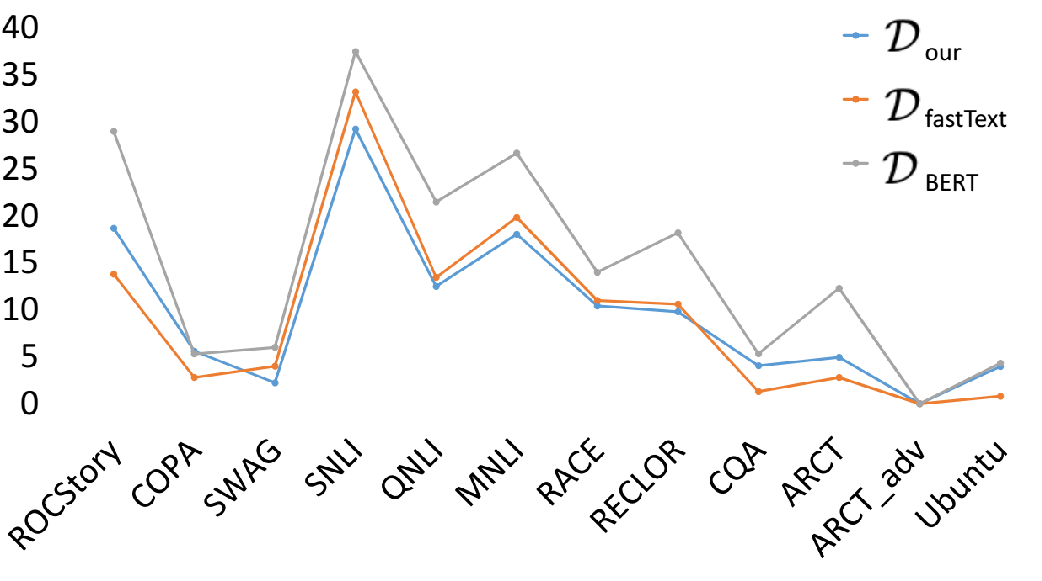
\includegraphics[width=0.65\columnwidth]{figures/iconip/d_figure.pdf}
    \caption{所有12个数据集上三种预测模型的偏差分数。}
    \label{fig4:d_figure}
    \end{figure}
综上所述,我们的方法有效地识别并量化了数据集中的偏差,并且与
仅假设模型的高度相关性进一步证明了我们方法的有效性和合理性。

\subsubsection*{数据集中偏差的揭示}
\textbf{为了更准确地识别那些存在问题的数据集},我们基于实验结果制定了一套详尽的标准。这
套标准的核心在于,如果一个模型在任何给定的线索特征上的偏差$\mathcal{D}$超
过10\%,我们就认定该数据集存在显著问题。这一简洁的评判标准使我们能迅速
辨认出那些含有严重统计线索问题的数据集。

在表\ref{tab4:best_acc}中,我们展示了四种简单分类模型在12个不同数据集上的最
高准确率,以及与多数选择(Majority)的偏差。这一表格详尽记录了使用词语线索
特征时,在各数据集上的选择结果。


\begin{table}[th]
    \small
    \centering
    \begin{tabular}{lcccccc}
    \toprule
    \textbf{数据集} &多数选择 & \multicolumn{2}{c}{Word Cues}  \\ \midrule
                                         & (\%)                 &  Acc.(\%) & $\mathcal{D}(\%)$ \\ \midrule
    ROC & 50.0            & 68.68          & \textbf{18.68}   \\
    COPA        & 50.0           & 55.60           &  5.60                \\
    SWAG       & 25.0           & 27.23           &   2.23                \\
    SNLI          & 33.33      & 62.57           &  \textbf{29.24}      \\
    QNLI         & 50.0           & 62.49            &  \textbf{12.49}   \\
    MNLI         & 33.33      & 51.37            &\textbf{18.04}        \\
    RACE        & 25.0          & 35.42            &   \textbf{10.42}   \\
    RECLOR       & 25.0           & 34.80            &   9.80   \\
    CQA          &20.0            & 23.42            &  3.42      \\
    ARCT        & 50.0            & 54.95           &  4.95      \\
    STS& 50.0           &50                 &0.0      \\
    Ubuntu   & 1.0               &4.96              &3.96      \\
    \bottomrule
    \end{tabular}
    \caption{\label{tab4:best_acc} 我们的四种简单分类模型在12个数据集上的最高准确率和与多数选择的偏差。}
    \end{table}

根据这个标准,我们识别出ROCStories、SNLI、MNLI、QNLI、RACE和RECLOR等
数据集存在大量统计线索问题。如表所示,这些数据集中的$\mathcal{D}$值显著高
于10\%的阈值,表明它们包含大量可以被模型利用的虚假统
计线索。例如,在ROCStories数据集中,我们的方法实现的最高准确率比随机选择高
出20.92\%,而在SNLI数据集中,这一比例甚至高达33.59\%。这进一步证明了这些数据集中存在的问题。

另外,我们也观察到,在未经过对抗性过滤且受到人为干预的数据集,例如
ARCT,存在更多的虚假统计线索。在对ARCT数据集进行的人工调整中
,我们发现准确率有显著变化(从54.95\%降至50\%),这表明人为干预对数据集质量的影响。
    
综上所述,在表格中我们报告了四种简单分类模型在12个数据集上的最高准
确率以及与多数选择的偏差。我们的发现表明,偏差$\mathcal{D}$是一个有效的工具,可
以用来识别和评估数据集中存在的词语线索问题。

总的来说,我们对问题数据集的深入分析和标准化方法,能够帮
助研究人员识别出含有大量统计线索问题的数据集。这一关键洞见将有
助于发展更加健壮的模型,使其不那么依赖于表面的统计线索,而是能够更深入地理解和处理复杂的数据。


\subsubsection*{2. 模型推理能力的评估}

\textbf{为了探究模型是否学习了数据集中的线索特征},并因此做出有偏见的选择,
本研究提出了一种方法来评估模型是否受到数据集中线索的影响。我们假设,
如果一个模型确实受到这些线索的影响,那么它在简单和困难部分的表现将会有所不同。
这种表现上的差异被称为\textbf{性能差距},它反映了模型的健壮性。
一个健壮的模型,理论上应当对虚假信息不敏感,并在简单和困难两部分的测试中
表现出类似的性能。尤其是在困难部分的表现,是衡量模型能力的一个重要指标。

%表\ref{tab4:gap_acc}展示了三种不同的模型——BERT、ESIM和FastText——在六个数据集上的
%性能差距。表格中的数据显示了这些模型在简单和困难测试部分上的表现差异,突出
%了各模型对线索特征的敏感程度。

\begin{table}[th]
    \small
    \centering
    \begin{tabular}{ccllll}
    \toprule
    数据集                                     & \multicolumn{1}{c}{模型} & \multicolumn{1}{c}{原始测试} & \multicolumn{3}{c}{线索分类}                                                                                        \\ \midrule
                                                 &                            & \multicolumn{1}{c}{(\%)}      & \multicolumn{1}{c}{简单} & \multicolumn{1}{c}{困难} & \multicolumn{1}{c}{\textbf{差距}} \\ \midrule
    \multicolumn{1}{c}{\multirow{3}{*}{SNLI}}   & BERT                       & \multicolumn{1}{l}{90.48}    & 94.99                         & 83.02                         & 11.97                         \\
    \multicolumn{1}{c}{}                        & ESIM                       & \multicolumn{1}{l}{87.44}    & 93.27                         & 77.77                         & 15.50                         \\
    \multicolumn{1}{c}{}                        & FastText                   & \multicolumn{1}{l}{54.74}    & 73.16                         & 24.23                         & 48.93                        \\ \midrule
    \multicolumn{1}{c}{\multirow{3}{*}{MNLI}}   & BERT                       & \multicolumn{1}{l}{85.10}    & 90.60                         & 79.30                         & 11.30        \\
    \multicolumn{1}{c}{}                        & ESIM                       & \multicolumn{1}{l}{76.82}    & 85.80                         & 67.34                         & 18.46                    \\
    \multicolumn{1}{c}{}                        & FastText                   & \multicolumn{1}{l}{47.15}    & 66.88                         & 26.31                         & 40.56                    \\ \midrule
    \multicolumn{1}{c}{\multirow{3}{*}{QNLI}}   & BERT                       & \multicolumn{1}{l}{88.89}    & 90.92                         & 85.54                         & 5.37             \\
    \multicolumn{1}{c}{}                        & ESIM                       & \multicolumn{1}{l}{72.17}    & 78.55                         & 61.66                         & 16.89                \\
    \multicolumn{1}{c}{}                        & FastText                   & \multicolumn{1}{l}{66.33}    & 80.94                         & 42.26                         & 38.67                 \\ \midrule
    \multicolumn{1}{c}{\multirow{3}{*}{ROC}}    & BERT                       & \multicolumn{1}{l}{90.54}    & 93.53                         & 84.01                         & 9.52             \\
    \multicolumn{1}{c}{}                        & ESIM                       & \multicolumn{1}{l}{65.42}    & 72.49                         & 50.00                         & 22.49                  \\
    \multicolumn{1}{c}{}                        & FastText                   & \multicolumn{1}{l}{62.91}    & 71.16                         & 44.90                         & 26.26                 \\ \midrule
    \multicolumn{1}{c}{\multirow{3}{*}{RACE}}   & BERT                       & \multicolumn{1}{l}{90.54}    & 93.53                         & 84.01                         & 9.52                           \\
    \multicolumn{1}{c}{}                        & ESIM                       & \multicolumn{1}{l}{65.42}    & 72.49                         & 50.00                         & 22.49                       \\
    \multicolumn{1}{c}{}                        & FastText                   & \multicolumn{1}{l}{62.91}    & 71.16                         & 44.90                         & 26.26                        \\ \midrule
    \multicolumn{1}{c}{\multirow{3}{*}{RECLOR}} & BERT                       & \multicolumn{1}{l}{48.40}    & 61.68                         & 41.74          & 19.93         \\
    \multicolumn{1}{c}{}                        & ESIM                       & \multicolumn{1}{l}{40.40}    & 52.69                         & 34.23                         & 18.46                 \\
    \multicolumn{1}{c}{}                        & FastText                   & \multicolumn{1}{l}{31.60}    & 43.11                         & 25.83                         & 17.29                          \\ 
    \bottomrule
    \end{tabular}
    \caption{\label{tab4:gap_acc} 模型在简单和困难测试数据集上的性能差距(\%)。}
    %模型捕捉单词的分布分数作为线索特征进行决策。}
    \end{table}

我们评估了3个典型的模型——BERT~\cite{devlin2018bert}、ESIM~\cite{chen2017enhanced}和FastText~\cite{joulin2017bag}——在6个``差''数据集上的表现,分别代表不同的复杂性层级:

\textit{FastText}: 这个模型将句子视为n-gram的集合,并试图独立预测每个答案的正确概率。在
这个模型中,单词的表示是基于300维的GloVe嵌入。在多项选择的设置中,FastText选择
得分最高的答案作为预测结果。由于其简单的结构,FastText在处理文本时可能更依赖于表
面的词汇特征,这可能导致在复杂的推理任务中性能不足。

\textit{ESIM}: 这个模型通过引入局部推理建模来增强其性能。它在两个片段局部对齐后,对前提和假
设之间的推理关系进行建模。我们使用GloVe嵌入对自己的ESIM模型进行训练,并选择得分最高
的答案。ESIM通过在前提和假设之间建立更复杂的关系来处理任务,这使其在处理需要深层次理
解的任务时表现更好。

\textit{BERT}:BERT模型基于Transformer架构,这是目前深度学习领域非常流行的一种结构。它的训练是在两个无监督的任务上进行的,
这两个任务分别是:遮蔽语言模型(MLM)和下一句预测(NSP)。这些
训练是在BooksCorpus和英文维基百科的文本上完成的。有多种预训练的
BERT模型可用,它们在层数和参数数量上有所不同。我们选择的是一
个基础版本,具有12层Transformer块、768个隐藏单元和12个自注意力头,共计110M个参数。
BERT对前提和假设的连接(带有分隔符)进行了3个周期的微调,以预测基于前提和假设的关系。
BERT的这种架构使其能够在处理需要广泛上下文理解和复杂推理的任务时表现出色。


这些模型在不同数据集上的表现及其在简单和困难部分之间的差距如\tabref{tab4:gap_acc}所示。简单和困难部分之间的差距通常在10-50%之间。
相比之下,人类在困难集上仍然能够保持良好的表现,这表明这些模型可能在某种程度上都受到了各自数据集中统计线索的影响。``组合''意味着我们汇总了由词语线索做出的选择。
对于``组合''而言,简单部分是其他两个线索特征简单部分的并集,而困难部分是两个其他困难部分的交集。我们发现``组合''通常会导致更大的差距。

在对比三个模型的性能差距时,我们发现BERT、ESIM和FastText的差距依次增大。
例如,FastText在SNLI数据集上的性能差距高达48.93\%,而BERT为11.97\%。这表明BERT可能
比其他两个模型更具健壮性。然而,所有模型在六个数据集上的性能差距均超过了10\%,这暗示
即便是BERT也受到了数据集中线索的影响。

值得注意的是,最高分数的模型并不总是最稳定的。例如,在RACE和RECLOR数据
集上,尽管BERT的整体准确率更高,但它的性能差距比其他模型更大。ESIM在RACE
上的差距相对较小,但考虑到其在困难测试数据上的表现接近随机选择,我们不能简
单地认为ESIM更优。此外,ESIM在RACE和RECLOR数据集上表现出较大的收敛困难。

综合来看,我们提出了一种新的模型评估方法,即通过困难数据测试来考察模型的准确率和
健壮性。通过性能差距分析,我们可以深入理解模型的局限性,并努力改进它们。通过减少性
能差距,我们可以开发出即使在具有挑战性情境下也能保持高性能的更健壮模型。

\subsubsection{微观结果分析}
\label{sec4:experiment2}


\begin{table}[htbp]
   \centering
    \scriptsize
    \begin{tabular}{p{0.09\textwidth}
    >{\centering}p{0.10\textwidth}
    >{\centering}p{0.08\textwidth}
    >{\centering}p{0.08\textwidth}
    >{\centering}p{0.08\textwidth}
    >{\centering}p{0.08\textwidth}
    c}
    \toprule
    数据集 & Top Cues & Cueness & FT  & ES & BT & RB\\ 
        &	& \%	& ($\Delta$)& ($\Delta$)& ($\Delta$)& ($\Delta$) \\ \hline
    \multirow{5}{*}{SNLI} 
    & ``sleeping'' & 13.95 & 30.3 &6.81 & 5.34& 4.87 \\                                                                    
    & ``no'' & 13.33 & 18.09 &3.32 & 2.05& 2.6 \\
    & ``because'' & 9.24 & 18.89 &4.88 & 5.61& 4.31 \\
    & ``friend'' & 8.82 & 22.96 &6.66 & 3.51& 3.05 \\
    & ``movie'' & 7.73 & 16.64 &0.06 & 9.47& -0.19 \\
           \midrule 
    \multirow{5}{*}{QNLI} 
    & ``dioxide'' & 4.52 & 9.78 &-0.06 & 4.97& 10.56 \\                                                                    
    & ``denver'' & 4.26 & 13.59 &7.14 & 2.23& 3.11 \\
    & ``kilometre'' & 4.24 & 4.85 &6.43 & 4.67& 2.55 \\
    & ``mile'' & 3.95 & 7.16 &15.64 & -1.65& -6.65 \\
    & ``newcastle'' & 3.8 & 3.44 &12.0 & 0.89& -1.23 \\
           \midrule 
    \multirow{5}{*}{MNLI} 
    & ``never'' & 10.4 & 29.15 &26.41 & 9.86& 10.6 \\                                                                      
    & ``no'' & 8.98 & 19.49 &20.17 & 1.2& 3.32 \\
    & ``nothing'' & 8.98 & 25.5 &26.84 & 5.11& 4.32 \\
    & ``any'' & 6.79 & 20.4 &19.39 & 7.76& 3.74 \\
    & ``anything'' & 5.73 & 18.43 &15.74 & 3.31& 1.14 \\
           
    \midrule 
    \multirow{5}{*}{ROC} 
    & ``threw'' & 12.99 & 1.28 &4.69 & 10.88& 0.97 \\                                                                      
    & ``now'' & 8.68 & -10.01 &14.51 & 1.75& 5.69 \\
    & ``found'' & 8.16 & -2.31 &4.45 & 5.12& -3.13 \\
    & ``won'' & 7.71 & 2.43 &0.74 & 1.05& 5.51 \\
    & ``like'' & 7.3 & 4.77 &10.06 & 8.81& 1.67 \\
           \midrule 
    \multirow{5}{*}{COPA} 
    & ``went'' & 3.61 & -10.83 &6.46 & 7.92& 1.04 \\                                                                       
    & ``got'' & 2.74 & 5.45 &-9.89 & -12.52& -10.3 \\
    & ``for'' & 2.14 & 10.11 &-1.89 & 9.05& 11.58 \\
    & ``with'' & 1.38 & -15.64 &-6.98 & 3.3& 13.82 \\
    & TYPO & 0.84 & -12.46 &-2.33 & 3.8& -8.22 \\
           \midrule 
    \multirow{5}{*}{SWAG}
    & ``football'' & 7.38 & 6.13 &8.55 & 1.2& 1.55 \\
    & ``anxious'' & 6.65 & 7.55 &-4.67 & -6.66& -1.67 \\
    & ``concerned'' & 6.19 & 12.6 &4.58 & 8.27& -5.66 \\
    & ``skull'' & 5.73 & -2.77 &0.49 & 8.43& 3.49 \\
    & ``cop'' & 5.01 & 2.79 &5.3 & -0.92& -0.04 \\
           \midrule 
    
    \multirow{5}{*}{RACE} 
    & ``above'' & 13.74 & 8.73 &-8.43 & -0.22& -1.92 \\                                                                    
    & ``b'' & 12.84 & 16.97 &-4.8 & 3.52& -3.45 \\
    & ``c'' & 11.83 & 15.69 &-6.94 & 8.6& -7.6 \\
    & ``probably'' & 6.77 & 9.91 &-0.06 & -3.8& 2.86 \\
    & ``may'' & 4.2 & 7.75 &-3.45 & -6.67& -1.8 \\
           
           \midrule 
    \multirow{5}{*}{RECLOR} 
    & ``over'' & 2.07 & 1.76 &-2.94 & -1.35& -4.12 \\                                                                      
    & ``result'' & 1.97 & -3.29 &-2.69 & -1.78& -3.7 \\
    & ``explanation'' & 1.81 & -6.33 &-1.73 & -2.76& -7.24 \\
    & ``proportion'' & 1.68 & -5.64 &-4.69 & 2.37& -2.16 \\
    & ``produce'' & 1.4 & 4.54 &-2.98 & -14.36& -3.7 \\
           \midrule 
    \multirow{5}{*}{ARCT} 
    & ``not'' & 3.74 & -2.54 &7.45 & -0.97& -11.96 \\                                                                      
    & NEGATION & 2.85 & 3.49 &10.04 & 6.28& -8.23 \\
    & ``n't'' & 2.52 & 10.3 &5.89 & 9.49& 4.84 \\
    & ``always'' & 2.25 & -4.66 &38.21 & -4.35& -8.26 \\
    & ``doe'' & 2.06 & -0.73 &-3.69 & -1.15& -7.22 \\
           \midrule 
    STS& OVERLAP & 1.96e-10 & 1.65 &-0.25 & 2.73& 0.57 \\ \midrule
    \multicolumn{3}{c|}{$\sum(|.|)$ (Model weakness)} 	& 469.8 & 361.4 & 227.7 & 216.2 \\
    \bottomrule 
    \end{tabular}
    \caption{数据集、每个数据集的前5个线索和每个模型在这些线索上的准确率偏差$\Delta$。}
    \label{tab4:bias}
    \end{table}
    %\clearpage
    在节中,我们将重点讨论关于线索发现、
模型探测和分析的成果以及有关ChatGPT模型评估的案例分析。
这一整套框架已经在我们的在线演示中得到实现和展示。

\subsubsection*{1. 数据集中的线索发现} 

我们利用在\secref{sec4:approach2}中描述的方法,对不同数
据集中的线索进行了识别和分析。具体来说,我们首先运用本研究定义的各种特征,
对每个数据集的训练和测试数据进行筛选。在\tabref{tab4:bias}的左半部分,我们展示了每个
数据集中发现的前五个主要线索及其相应的线索得分。

以STS数据集为例,这是一个经过精心平衡的对抗性数据集,我
们在其中只识别出一个线索——OVERLAP,且该线索的得分非常低。这一发现并不出
乎意料,因为OVERLAP作为我们列出的特征中唯一涉及前提和假设标记的``二阶''特征
,很可能已经避开了数据创建者创造的偏见。

在大多数情况下,我们发现的主要线索都是词汇特征。除了OVERLAP之外,
我们还在列表中发现了如NEGATION和TYPO等特征。有趣的是,当我们将关注
的线索扩展到前十个时,情感(SENTIMENT)和命名实体识别(NER)特征也显
现出来。值得注意的是,我们还发现了一些以往其他研究报告中提到的、被认为
有偏见的特征,比如ARCT中的``not''和NEGATION,MNLI和SNLI中的``no'',以
及ROC中的``like''。尤其在MNLI数据集中,我们发现所有五个识别出的线索都与负
面词汇相关,这表明该数据集可能包含了显著的人为痕迹,从而可能导致模型的脆弱性。

此外,我们还注意到某些词汇线索揭示了问题中的特定句法、语义或情感模式。例如,SNLI
数据集中的``because''表明了因果关系的存在;ROC中的``like''通常与积极情感相关
;RACE中的``probably''和``may''表达了不确定性等。这些发现可作为修订数据集时的重要线索。

\subsubsection*{2. 模型偏见的探测和分析}
为了深入探索模型是否受到数据集中特定线索或特征的影响,我们在
原始训练集上对四种模型——FastText、ESIM、BERT和RoBERTa——进行了训练。与
之前的宏观测试相比,我们新增了RoBERTa模型的研究。作为BERT的改进版本,RoBERTa通过
在更大的数据集上训练、增加批量大小,并去除了一些原始BERT的目标,例如下一句预测(NSP),从
而显著提高了性能。这些改进使得RoBERTa在多种自然语言处理任务上表现更加出色。我们选用的
是RoBERTa的基础版(base version)进行测试。接下来,我们通过准确性和分布测试来评估这些模型。

\subsubsection*{准确性测试}
我们在\tabref{tab4:bias}中展示了测试结果。如\ref{sec4:accuracytest}所
述,$\Delta$值的正负号表示模型在含有和不含特定特征的数据子集之间性能变化的方
向。$\Delta$的绝对值大小则反映了模型性能受这些特征影响的程度。较大的$\Delta$值表
明模型对特定特征有更强的依赖或敏感性,而较小的值则意味着模型更加健壮。

在\tabref{tab4:bias}的底部,我们观察到,跨越所有十个
数据集,$\Delta$绝对值的总和遵循以下顺序:RoBERTA $<$ BERT $<$ ESIM $<$ FastText。这
与我们之前的假设和社区对这些模型的普遍看法一致。然而,对单个数据集和特征的细致检查揭示
了更复杂的情况。例如,FastText倾向于捕捉单词级的线索,而不是深层次的语义线索,而像BERT和
RoBERTa这样的更复杂模型则对结构性特征(如NEGATION和SENTIMENT,实际上是词汇类别)更
敏感。这种差异可以通过FastText的设计理念来解释,它更专注于单词层面,而不是句法或语义结构。

有趣的是,FastText对TYPO特征显示出了强烈的负相关性。我们推测,这可能是因
为FastText使用了更规范的词汇进行训练,因此对于文本中的拼写错误表现出了较低的容忍度。

\subsubsection*{分布测试}
\begin{figure}[th]
    \centering
    \begin{minipage}[b]{0.45\linewidth}
    \centering
    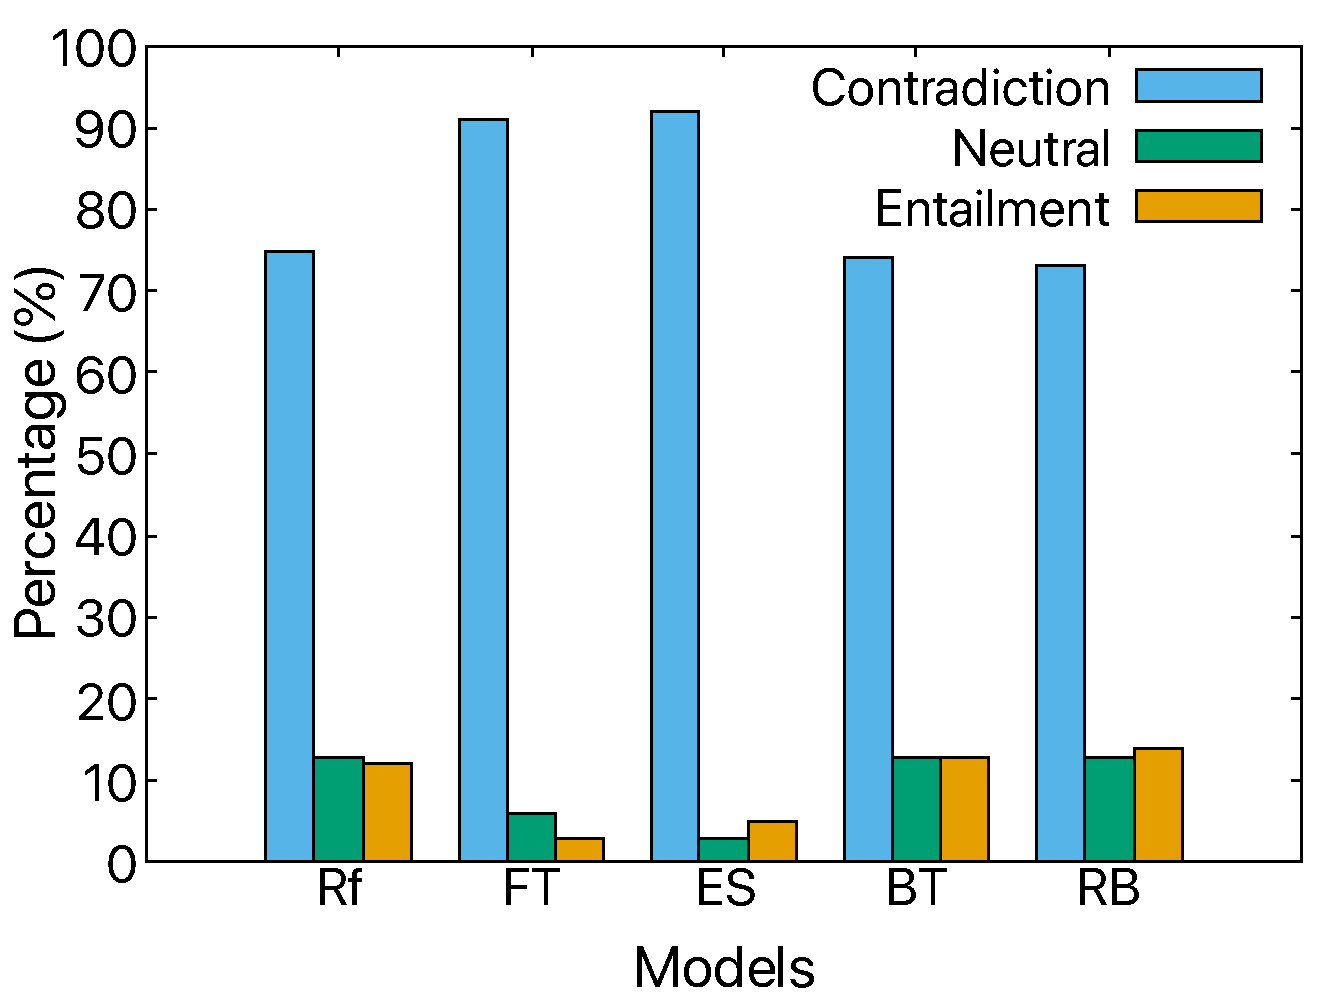
\includegraphics[width=\columnwidth]{figures/emnlp/no-mnli.pdf}
    \caption*{MNLI中的线索``no''} 
    \label{fig4:cue_no} 
    \end{minipage}
    \hspace{0.5cm} 
    \begin{minipage}[b]{0.45\linewidth} 
    \centering 
    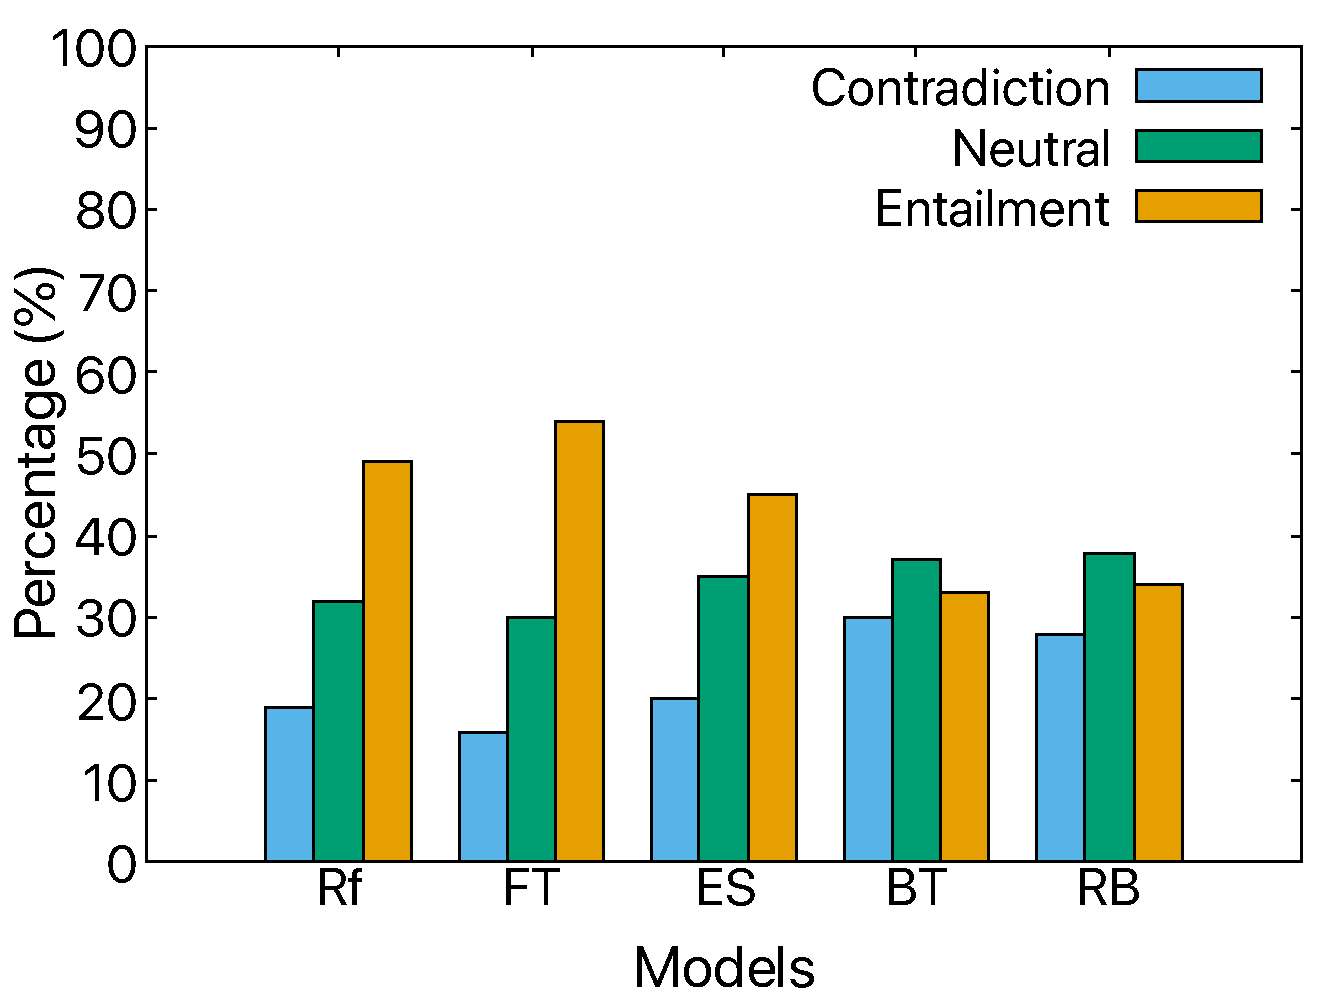
\includegraphics[width=\columnwidth]{figures/emnlp/speaking-snli.pdf} 
    \caption*{SNLI中的线索``speaking''}
    \label{fig4:cue_speaking}
    \end{minipage}
    
    \vspace{0.5cm}
    
    \begin{minipage}[b]{0.45\linewidth}
    \centering
    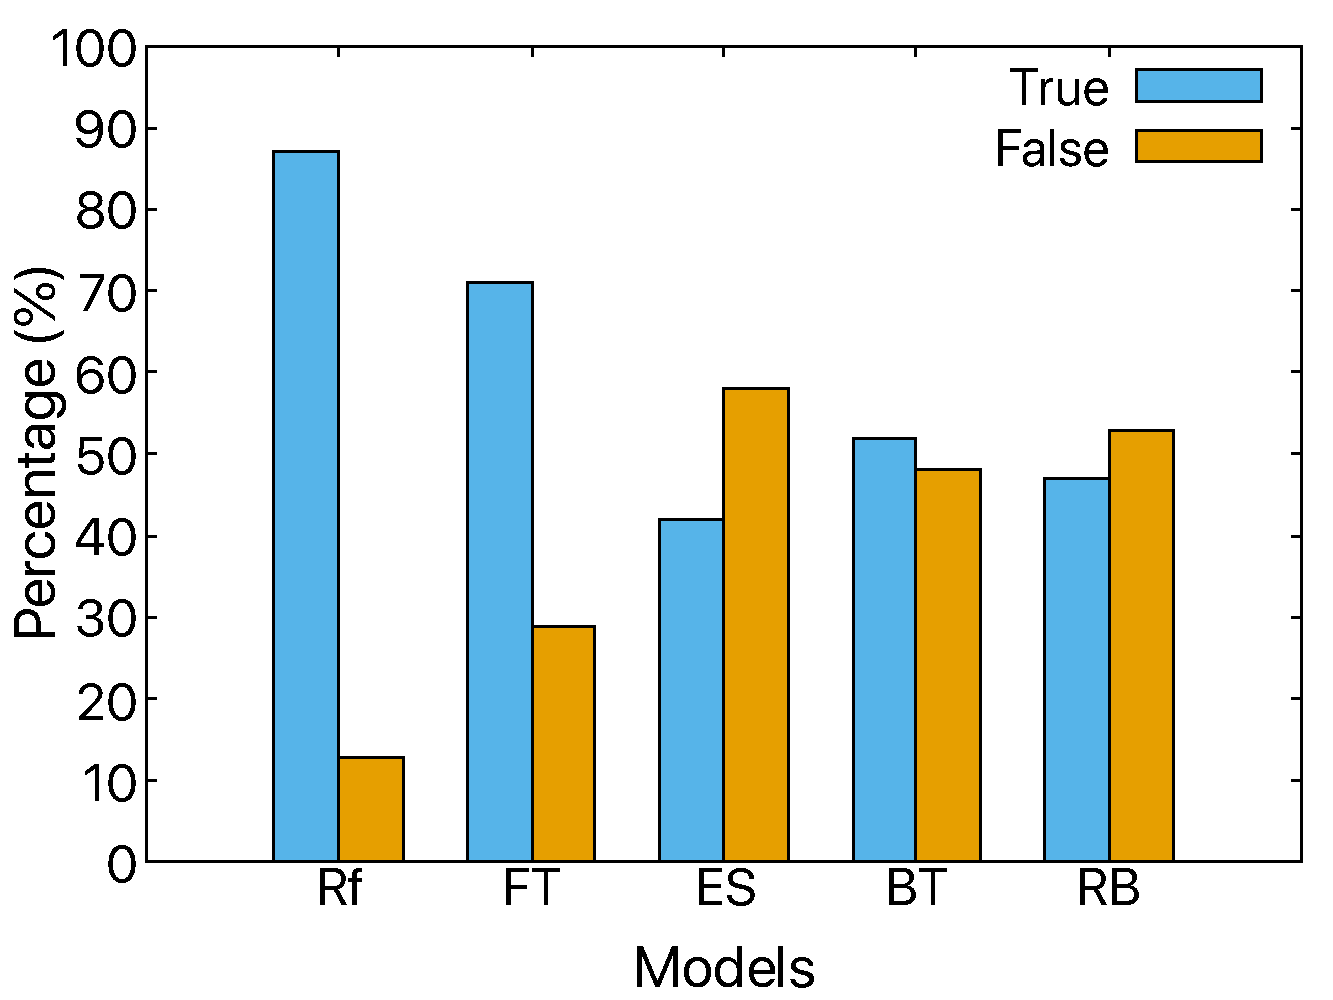
\includegraphics[width=\columnwidth]{figures/emnlp/above-arct.pdf}
    \caption*{ARCT中的线索``above''} 
    \label{fig4:cue_above} 
    \end{minipage}
    \hspace{0.5cm} 
    \begin{minipage}[b]{0.45\linewidth} 
    \centering 
    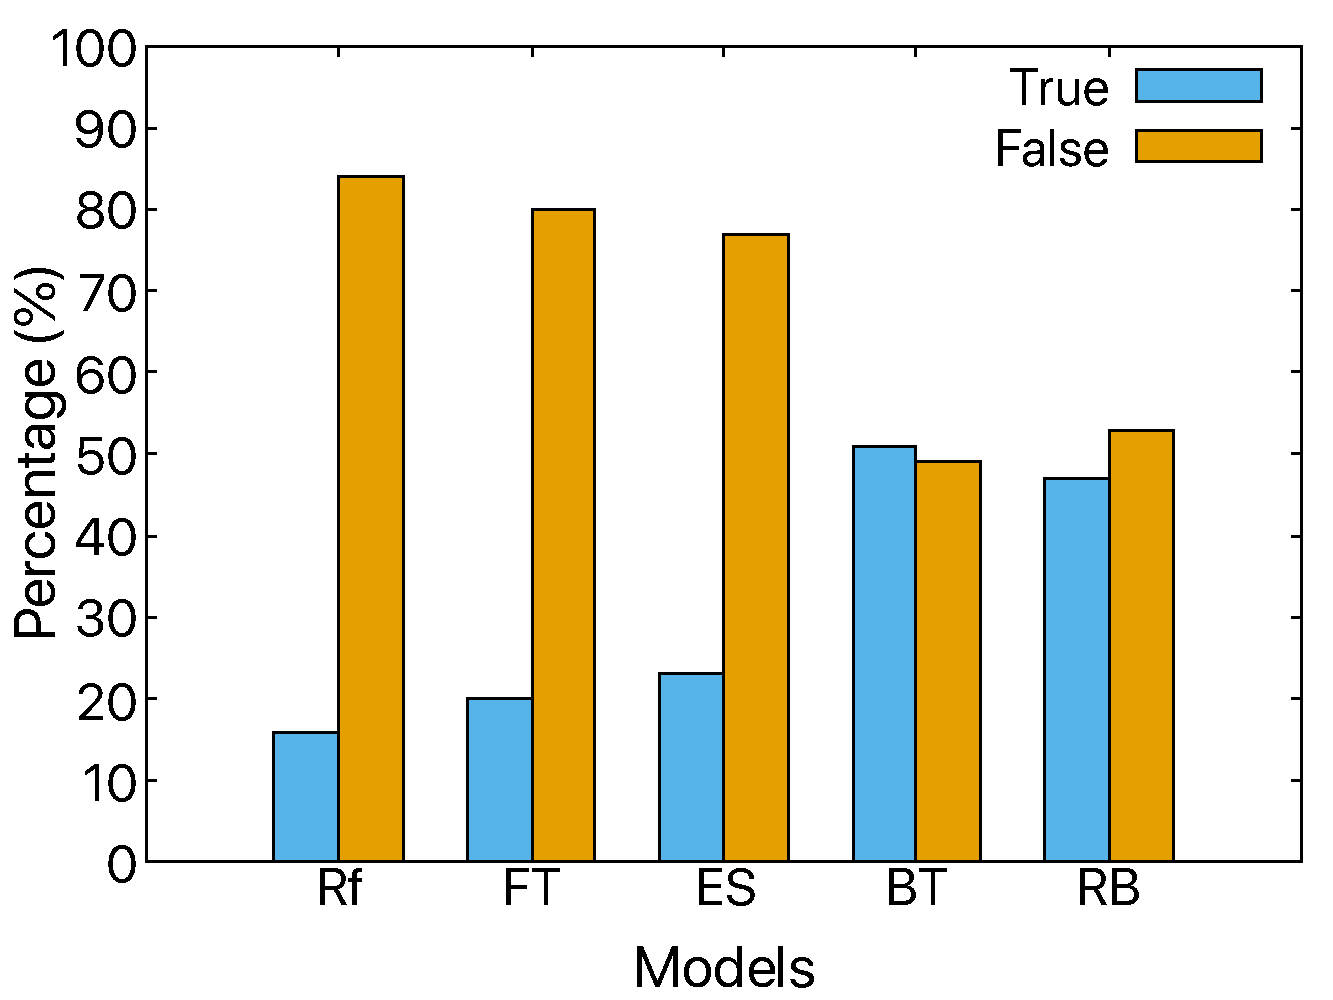
\includegraphics[width=\columnwidth]{figures/emnlp/threw-roc.pdf} 
    \caption*{ROC中的线索``threw''}
    \label{fig4:cue_threw}
    \end{minipage}
    \caption{四个不同模型的分布测试示例。}
    \label{fig4:cue_result}
    \end{figure}

在\figref{fig4:cue_result}中,我们展示了三个引人关注的发现。这些
柱状图代表了四个模型基于每个预测标签的分布百分比。$R_f$表示具有特定特征的训
练数据分布。我们注意到,在MNLI数据集中的``no''线索上,所有模型在\tabref{tab4:bias}中均获
得了正$\Delta$值,尤其是FastText。与准确性测试一致,我们发现在有``no''线索的情况
下,FastText和ESIM的预测标签分布偏差在\figref{fig4:cue_result}中得到了加强。它们
更倾向于预测``矛盾''类别,甚至超过了训练数据中的基线。与此相比,BERT和RoBERTa的预
测分布更加适度地遵循了训练数据。

尽管``no''线索在影响模型方面表现出一定的有效性,但``above''这一线索却并不那
么成功。\figref{fig4:cue_result}显示,在ARCT数据集中,ESIM的预测结果
分布与训练数据完全相反,这解释了\tabref{tab4:bias}中的$\Delta$值为-8.43,并
暗示即使数据中存在线索,模型也可能不会利用它。同样,BERT和RoBERTa在``speaking''线索
上的低$\Delta$值也解释了它们在\tabref{tab4:bias}中的表现。

特别地,``threw''线索为BERT提供了一个例外情况,因为在分布测试中的结果与准确性测试不一致:
尽管BERT在准确性偏差上表现很高,但其预测分布却相对均匀。我们并没有遇到很多这样的矛
盾情况。然而,当这种情况确实发生时,如在这个例子中,我们认为BERT可能没有真正利用``threw''这一
线索。

通过上述分析,我们不仅揭示了数据集中的线索和特征,还展示了这些线索对不同模型性能的影响。这
些发现为深入理解模型行为提供了宝贵的洞见,并为未来的数据集设计和模型开发提供了重要的指导.

\subsubsection*{3. 案例研究}
\label{sec4:mitigatingbiases}
\begin{figure*}[th]
\centering
\includegraphics[width=0.9\columnwidth]{figures/emnlp/prompt.eps}
\caption{提示语(prompt)。}
\label{fig4:prompt}
\end{figure*}
最近,OpenAI发布的大型语言模型(LLM)ChatGPT在自然语言处理(NLP)领
域引起了极大关注。ChatGPT,属于GPT-x系列模型\footnote{目前x的值为3.5或4,在我们的实验中,使用的是基于GPT-3.5的版本)}之一,
采用了类似InstructGPT\cite{ouyang2022training}的训练方法,即通过强化学习从人类反馈中学习(RLHF)。

在本节中,我们关注的是ChatGPT在零样本情况下是否受到偏见特征的影响。
具体来说,我们选择了一个聚焦于MNLI数据集中``no''一词的案例研究。我们的
目标是评估不同提示语的有效性,并基于这一单一偏见特征选择最佳提示语,以减轻偏见。

\subsubsection*{数据集}
\label{sec3:chatgptdata}
我们从MNLI数据集中挑选了测试实例,专注于``no''一词对ChatGPT性能的影响。
原始测试集包括3240个矛盾实例(Contradiction)、3463个蕴涵实例(Entailment)和3129
个中立实例(Neutral)。
含有``no''的实例分布为:矛盾229个,蕴涵38个,中立46个。

为了测试准确性,我们选取了所有含有``no''的313个实例,并从未包含``no''的测试集
中随机挑选了相同数量的实例,以确保评估的平衡性。

在分布测试中,我们从每种分类标签中各选取了38个含``no''的实例,共计114个。

\subsubsection*{提示语}
如图\ref{fig4:prompt}所示,我们设计了四种提示语。第一种由 ChatGPT 自行生成,
我们询问它关于 MNLI 任务的最佳提示语是什么,并得到了Prompt 1。
第二种提示语受到先前工作~\cite{qin2023chatgpt}的启发。
第三和第四种提示语在前两种提示语的基础上加入了``Let’s think step by step''\cite{kojima2022large}的元素,
采用了``思维链''(Chain of Thought, CoT)的方法,这种修改方式在
提高 InstructGPT 在推理任务上的性能方面已被证明有效,如 Ouyang 等人在 2022 年的研究\cite{ouyang2022training}所示。


\subsubsection*{ICQ结果}
\label{sec3:chatgptacc}

\begin{table}[th]
\centering
\scriptsize
\begin{tabular}{c|ccc}
\toprule
\textbf{提示语} & 准确率(含``no'') & 准确率(不含``no'') & $\Delta Acc$ \\ \midrule
P1  & 74.34& 77.32& -2.98   \\ \hline
P2&  75.42& 74.18 & 1.24 \\ \hline
P1 + CoT  & 78.35& 77.28&1.07  \\ \hline
P2 + CoT&  76.67& 76.40&  0.27 \\ \hline
 \bottomrule
\end{tabular}
\caption{准确性测试结果(\%)。P1=提示语1,P2=提示语2。}
\label{tab4:accuracy}
\end{table}

\begin{figure}[th]
\centering
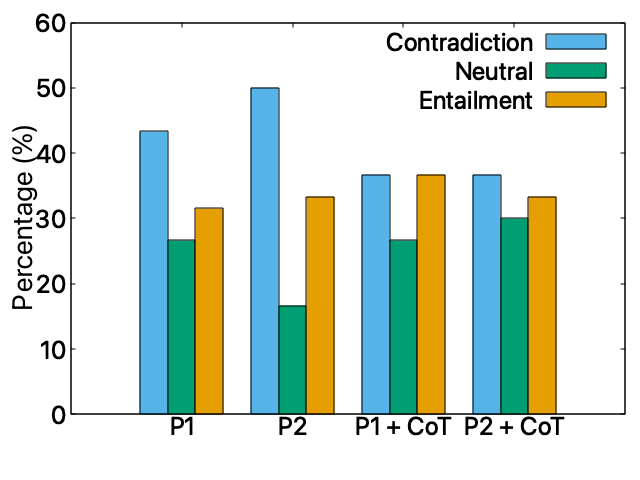
\includegraphics[width=0.6\columnwidth]{figures/emnlp/data/cue.png}
\caption{分布测试结果。}
\label{fig4:cue_chatgpt}
\end{figure}



我们使用不同的提示语对含有和不含有``no''的实例评估了模型的准确率。结果显示在\tabref{tab4:accuracy}中。
P1展示了负$\Delta$准确率,表明在存在``no''时难以泛化。
P2显示了正$\Delta$准确率,表明更好的泛化能力。
将``CoT''添加到两个提示语中都减少了偏见风险。
P1 + CoT在准确率(含``no'')方面显示了最显著的提升,但P2 + CoT有最小的绝对
$\Delta$准确率,表明对``no''的敏感性最低,是测试提示语中偏见风险最低的。

此外,我们分析了模型在不同提示语的压力测试集上的预测分布,如\figref{fig4:cue_chatgpt},该测试集包含了具有平衡标签分布的``no''一词。
分布测试结果揭示了P1和P2预测分布的不平衡,P1和P2倾向于预测矛盾。
添加``CoT''减轻了这些不平衡,导致更平衡的分布。
P2 + CoT在标签中呈现了最平衡的分布,支持其最低的偏见风险。

总之,我们的案例研究,特别是当关注``no''特征时,表明零样本ChatGPT可以受到偏见特征的影响。提示语的选择显著影响其性能。在评估``no''特征时,P2 + CoT在两项测试中显示了最低的偏见风险。``CoT''策略在减少这一特定特征的偏见风险方面似乎是有效的。然而,重要的是要注意,我们的发现,特别是关于``no''特征,表明ChatGPT推荐的自我提示语(P1)可能并不总是最优的。这强调了人类干预和持续探索的重要性,以优化性能并最小化偏见风险。未来的研究和结论将受益于更细致和针对特定特征的分析。

        

\subsection{本章小结}

在本章节的小结中,我们深入剖析了常识性推理模型鲁棒性不足的核心问题,并探讨了这一现象背后的深层原因。我们着重分析了模型在学习过程中缺乏人类的稳固推理能力,探求了模型究竟学习到了什么。为了深入理解这一问题,我们引入了两种创新的测试框架,目的是对相关问题进行更精细的分析与理解。

鉴于模型性能与数据密切相关,我们从宏观和微观两个角度出发,对数据中的偏见线索及模型的偏见进行了全面的评估和分析。在宏观层面,我们开发的测试框架通过对不同数据集上基于统计特征的简单分类模型的最高准确率进行评估,以及通过与多数选择(Majority)的偏差值来评估数据集中存在的偏差特征程度。我们将测试数据划分为简单(easy)和困难(hard)两类,以量化评估模型在识别和处理虚假特征方面的能力。这一方法揭示了模型对某些统计规律的过度依赖,有助于我们深入理解模型泛化能力的限制。

在微观层面,我们设计了ICQ(``I-see-cue'')框架。我们首先通过结合特征的分布不平衡性和训练集与测试集分布的相似性来定义``cueness score'',从而发现可能影响模型的关键特征,并评估数据集中存在的问题。ICQ通过多维特征划分和细致的性能分析,探究模型在不同特征上的准确性和分布表现。此外,我们还开发了一种直观的可视化工具,以更有效地识别和理解模型性能差异的根源。

值得一提的是,在微观分析中,我们还对ChatGPT进行了案例分析,证明了ICQ框架的广泛适用性,能够为多种模型提供深入的分析。

总体而言,本研究的主要贡献在于这两种高度创新的分析框架,它们为深入理解和提升常识性推理模型的鲁棒性开辟了新途径。通过结合宏观与微观方法,我们能够全面评估模型在处理复杂数据时的行为模式,特别是在识别潜在虚假特征方面的能力。这些成果不仅揭示了模型的潜在薄弱环节,也为未来设计更健壮、更可解释的人工智能系统奠定了一定的基础。
%iconip conclusion
%我们解决了自然语言理解和推理数据集中存在的统计偏差这一关键问题。我们提出了一个轻量级框架,
%自动识别多项选择自然语言理解(NLU)相关数据集中的潜在偏差,并评估为这些数据集设计的模型的健壮性。
%我们的实验结果证明了这一框架在检测数据集偏差和评估模型性能方面的有效性。此外,我们的方法在过滤有偏见的训练数据方面展现了潜力,
%从而促进了具有更强推理能力的模型的发展。

%作为未来的工作,我们计划进一步调查NLU数据集中偏差的本质,并探索更复杂的技术来检测和减轻这些偏差。
%此外,我们打算将我们的框架扩展到多项选择设置之外的其他类型的NLU任务。通过持续改进我们对数据集偏差及其对模型性能影响的理解,
%我们希望为开发更健壮、准确且可靠的NLU模型做出贡献,这些模型能够更好地泛化到现实世界应用中。

%我们的轻量级框架ICQ能够识别多项选择NLU数据集中的偏见和线索,从统计角度阐明模型行为。在多样化任务上的广泛实验验证了ICQ揭示数据集和模型偏见的效率。通过对ChatGPT的案例研究,我们探索了其线索,提供了实际指导。ICQ促进了我们对大型语言模型的理解和优化,推动了健壮、无偏见的人工智能系统的创建。

\newpage
\null
\newpage

\newpage
\fancyhead[LH]{上海交通大学学位论文}
\fancyhead[RH]{第五章\quad 提升推理模型鲁棒性的数据增强策略}
\setcounter{figure}{0}
\setcounter{table}{0}
\section{提升推理模型鲁棒性的数据增强策略}

在人工智能领域,常识性推理作为一项核心任务,其挑战在于赋予机器与人类相似的理解和决策能力。
尽管神经网络模型如BERT\cite{devlin2018bert}和RoBERTa\cite{liu2019roberta}
在ROC\cite{mostafazadeh2016corpus}、
COPA\cite{roemmele2011choice}、ARCT\cite{habernal2018argument}和RECLOR\cite{yu2020reclor}
等任务上取得了显著成就,它们在处理对抗性数据或不同于训练环境的场景时仍显脆弱。
这种局限性通常源于模型对数据集中特定模式的过度依赖,而非深入理解问题本
质\cite{naik2018stress,mccoy2019right,schuster2019towards,nie2020adversarial}。
在上一章对模型鲁棒性差的原因的解释中我们也验证了的确受到偏差数据的影响。

针对模型鲁棒性不足的问题,本章提出了一种数据增强方法,旨在提升常识性推理模型的鲁棒性。这
种方法通过创新的数据增强手段减少数据的简单统计偏差,从而增强模型的鲁棒性。

本研究的灵感来源于生物
学中的``交叉''和``变异''过程。这一策略模仿生物遗传中的染色体交叉和基因变异,
创造问题实例之间的新组合和变化。``交叉''操作涉及交换两个不同问题的选项,
而``变异''操作涉及对问题的某些部分进行微妙修改。这些操作产生新的、具有挑战
性的训练实例,促使模型超越表面的统计规律,深入学习问题的内在逻辑和结构。

这些策略被应用于领先的神经网络模型,并在多个基准数据集上进行
测试。实验结果显示,这些策略显著提高了模型在多样化和对抗性数据环境
中的鲁棒性,同时在标准测试集上保持或提升了性能。


\subsection{概述}
\label{sec3:intro}
选择题(MCQs)是一种常用的格式,
用于评估自然语言理解(NLU)能力,涵盖了因
果推理~\cite{roemmele2011choice}、故事结尾预
测~\cite{mostafazadeh2016corpus,huang20story}、论
证理解~\cite{habernal2018argument}以及阅读理解~\cite{yu2020reclor}等任务。
这些任务通常由一个情境描述(前提)和几个选择项组成。
例如,COPA 数据集~\cite{roemmele2011choice}通过 MCQs 
来测试常识性因果推理~\cite{luo2016commonsense},一个典型的例子如下:

\begin{example}\label{ex:copa}
    COPA 选择题示例:
    \begin{description}
        \item[Premise:] The man hurt his back.
        \item[Choice 1:] He stayed in bed for several days. \checksymbol
        \item[Choice 2:] He went to see a psychiatrist. \crosssymbol
        \end{description}
        \end{example}

近年来的研究开始探究高级神经模型在 NLU 推理问题上的强大表现。
特别是,研究发现许多模型可能并不是通过真正理解上下文与选项之间
的逻辑和语义联系来取得成功,而是通过利用训练和测试数据中的偏见或
统计特征。这一观点得到了``仅选项测试''(也称为``仅假设测试'')的
支持~\cite{sharma2018tackling,bras2020adversarial}。在这种测试中,
模型如 BERT 在没有前提的情况下也能正确回答问题。

我们将这种现象称为自然语言推理中的``短路''。虽然``仅假设测试''为短路行为
提供了一些证据,但我们认为它具有一定的局限性。即使模型在没有前提的情况下
能正确回答问题,也不一定意味着它在有前提时不会考虑前提。

为了更全面地测试这种``短路''现象,我们尝试了一种新方法:绘制模型在处
理完整问题时,最后编码层中单词间的注意力图。如图\ref{fig3:att-goodex}所示,
我们使用了来自 COPA(见\exref{ex:copa})的示例。注意力图清楚地展示了,在处理
完整问题时,模型对于第一个选项与前提之间的联系几乎没有关注,而当仅处理选项,无上下文时,
选项内单词之间的注意力保持不变。

\begin{figure}[th!]
\centering
\includegraphics[width=0.5\columnwidth]{figures/ecai/end_related.eps}
\caption{展示 BERT\cite{devlin2018bert} 在 COPA 问题上短路的注意力图。}
\label{fig3:att-goodex}
\end{figure}

尽管使用注意力图来手动检查模型的短路行为可以提供洞察,但这
一过程既繁琐又成本高昂。因此,我们开发了一种自动化的白盒测
试算法,使用阈值来模拟人类的视觉过程。但这种方法也有局限性:它
需要访问模型的内部代码,并且只适用于基于注意力的模型。

为了解决这些挑战,我们引入了一种新操作,称为``交叉'',用于 MCQ 问题实
例。这种操作通过交换两个 MCQs 的选项来模拟生物繁殖中的染色体交叉过
程。这对经常利用短路行为的模型提出了独特挑战,通过构建代理测试案例
可以在真实任务中检测这种行为。我们在三个最新的、强大的 NLU 推理模型上
进行了这种交叉测试,发现这些模型在实例级别的压力测试中表现出明显的
准确率下降,显示出短路行为。

在确认了短路行为的存在后,我们的目标是提高模型的鲁棒性。我们考虑了
使用挑战模型难度的压力测试生成更多训练实例的方法。但由于许多压力测
试对选项构建有限制,这限制了它们作为通用数据增强方法的有效性。然
而,交叉操作及其对应的``突变''操作提供了一个可行的解决方案。这些操作
不仅可以用于检测短路行为,还可以作为有效的数据增强技术,减少短路行为
的发生,从而提高 NLU 模型的整体鲁棒性。
为此,我们应用
交叉、突变和反向翻译~\cite{xie2020unsupervised}来增强 BERT、XLNet~\cite{yang2019xlnet} 和 RoBERTa~\cite{liu2019roberta} 在 ROC~\cite{mostafazadeh2016corpus}、COPA、ARCT~\cite{habernal2018argument} 和 RECLOR~\cite{yu2020reclor} 上的表现。
我们的实验显示,我们的方法让模型在压力测试上的准确性最多提高了多达 24\%,在原始测试数据上最多也提高了 10\%。

本研究主要贡献如下:

\begin{enumerate}
\item 我们提出了两种检测短路行为的方法:一种基于注意力权重阈值的白盒方法和一种受分子生物学启发的黑盒``交叉''测试。
\item 我们通过实验证实了三个强大、微调过的 NLU 推理模型中存在短路行为。
\item 我们建议使用交叉和突变操作来增强训练数据,鼓励模型考虑问题的上下文。我们的实验确认了这种方法的有效性,不仅在压力测试上,而且在原始测试数据上也显示出模型鲁棒性的显著提升。
\end{enumerate}

\subsection{相关工作}
\label{sec3:related}
我们的研究涉及四个个主要领域:虚假特征的影响、数据增强的有效性,数据集过滤的挑战和好处以及模型分析。

\subsubsection*{虚假特征的影响}
近期研究揭示了虚假特征在自然语言处理模型性能中的显著影响。具体来说,这些模
型倾向于依赖表面模式,例如词汇化特征(如n-gram及其交叉组合)和非词汇化特征(比如词汇重叠
、句子长度和BLEU分数)\cite{sharma2018tackling,srinivasan2018simple,zellers2018swag,bowman2015large,naik2018stress,joshi2022all}。
显著的一点是,某些NLP模型能够在多项选择问答任务中取得高准确率,即使它们没有
考虑上下文信息,这种现象通过``仅假设测试''暴露了模型对假设中细微但重要语义扰
动的不敏感性\cite{sanchez2018behavior,izmailov2022feature}。这些发现促
使我们直接对模型进行诊断,以减少仅依赖假设中的短路推理方式。

\subsubsection*{数据增强的应用和挑战}
数据增强技术已被广泛应用于增
强视觉和语言任务模型的鲁棒性~\cite{perez2017effectiveness,belinkov2017synthetic}。
然而,研究指出这种方法可能导致模型在增强数据集上过度拟合,从而限制了对新场景的泛
化能力~\cite{jia2017adversarial,ribeiro2018semantically,iyyer2018adversarial,liu2019inoculation,mccoy2019right}。我
们采用一种新策略,通过生成包含多样化``噪声''示例的增强数据,以防止模型过分依赖特定的虚
假线索。此外,我们还探索了一系列不依赖特定特征的增强方法,以降低模型依赖于选项短路推理的倾
向,这在以往研究中较少涉及~\cite{xie2020unsupervised,sennrich2016improving,cubuk2018autoaugment,cubuk2020randaugment,zhang2017mixup,feng2021survey}。

\subsubsection*{数据集过滤的挑战与创新}
在提升数据集质量的过程中,尝试通过移除某些人为特征来实现,但这种方法
可能过分依赖于模型本身的性能,从而影响其长期的稳定性和
可靠性~\cite{yaghoobzadeh2019robust, bras2020adversarial}。因此
,我们的研究中着重于开发一种创新策略,而非仅依赖于过滤现有数据集,以此提升
模型在处理复杂、真实世界数据时的鲁棒性和准确性。

\subsubsection*{模型分析}
自从大型预训练语言模型的出现,许多研究已经专注于分析这些模型的内
部机制,包括语言属性如何被编码在上下文化表示
和注意力头中~\cite{goldberg2019assessing,clark2019does,liu2019linguistic,tenney2019you}。与此相比
,我们的研究更加关注于模型的高级推理能力。我们通过设计挑战性数据集和执行所
谓的短路测试(一种压力测试),补充传统的挑战或基准数据集,从而测试模型是
否真正具备推理能力,尤其是在短路行为方面~\cite{belinkov2019analysis}。


%\subsection{短路现象代理测试和数据增强策略}
%\subsubsection{ecai概述}
%\label{sec3:approach}

%本节首先介绍我们用于测试模型短路的方法,然后修改部分方法以创建训练数据,以解决短路问题并增强模型的鲁棒性。
\subsection{短路问题的代理测试}
\label{sec3:approach1}
在这一节中,我们首先介绍了用于检测模型中短路现象的方法,
然后在下一节中我们对这些方法进行了一些修改,以便创建训练数据来解决短路问题并提高模型的鲁棒性。

由于目前没有现成的方法可以确切地证明模型在处理问题时是否发生了``短路'',我们设计
了两种作为短路代理测试的方法。这些方法能揭示模型是否倾向于采用短路的方式解决问题,
尽管它们不能直接证明短路本身,其作用类似于在天文学中对暗物质的探测。一种方法是在白
盒设置下检查模型的注意力图(Attention Weights, AW),另一种方法则是在黑盒设置下,通过对正确选项应用不同操作
来生成新的测试案例。
\subsubsection{白盒测试}

我们可以通过可视化基于注意力的模型的注意力图来直观地检测模型是否采用了短路。
考虑一个经过良好训练的模型和一个以 \textit{[CLS] 前提 [SEP] 选项 [SEP]} 格式正确回
答的多项选择题(MCQ),其中 \textit{[CLS]} 和 \textit{[SEP]} 是模型使用的分隔
符。在这种设置下,\textit{选项} 代表正确的选择。我们首先对输入进行分词处理,将这些
令牌序列输入到模型中,并从模型的最后一个编码器层提取所有注意力头的注意力图。

我们使用现成的工具\cite{vig2019multiscale}将注意力图可视化成用户友好的
形式,如\figref{fig3:att-goodex} 所示。然后,我们请人类注释者判断正确选
项到前提之间是否存在强的注意力连接。如果超过一半的注释者认为存在强连接,则
判断该 MCQ 没有采用短路解决。

%\begin{figure}[h!]
%    \centering
%    \includegraphics[width=0.6\textwidth]{example-image}
%    \caption{注意力图示例。}
%    \label{fig3:att-goodex}
%\end{figure}

虽然手动注释方法准确,但它成本过高,难以应用于大规模的测试。为了克服
这个问题,我们提出了一种基于规则的程序,自动检测模型在 MCQ 上的短路行为。具
体来说,我们通过对所有注意力头进行最大池化操作,将注意力图聚合成一个单一的图表
。然后,我们检查选项中的每个令牌与前提中的每个令牌之间是否存在至少
一个高于阈值 \( t_1 \) 的注意力分数,或至少两个高于阈值 \( t_2 \) 的分数。特
殊令牌如逗号和句号被排除在外。如果这两个条件都不满足,我们认为模型在这个 MCQ 上没
有发生短路。实践中,阈值 \( t_1 \) 和 \( t_2 \) 需要被调整以最大限度地模拟人类
的判断。相关的伪代码如下所示:

\begin{algorithm}
    \small
        \caption{注意力权重阈值}
        \label{AW}
    \hspace*{0.02in} {\bf Input:} 
    premise $P$, correct choice $C$, model $M$,  threshold $t_1$ and $t_2$. \\
    \hspace*{0.02in} {\bf Output:}
    binary 0/1 label $L$.
        \begin{algorithmic}[1]
            \State initialize counters $c_1$ and $c_2$ to 0.
            \State tokenize the formatted input as sequence of tokens $S$.
            \State feed $S$ into $M$ and extract the last layer's attention maps $Attn_{all}$.
            \State aggregate $Attn_{all}$ into $Attn_{max}$ by max-pooling over all attention heads.
            \For{$w_1$ in $C$}
            \For{$w_2$ in $P$}
            \If{$Attn_{max}(w_1, w_2)> t_1$}
                    $c_1$ += 1
            \EndIf
            \If{$Attn_{max}(w_1, w_2) > t_2$}
                    $c_2$ += 1
            \EndIf
            \EndFor
            \EndFor
            \State output 1 if $c_1>0$ or $c_2\geq 2$ and 0 otherwise.
        \end{algorithmic}
    \end{algorithm}
    
    这段伪代码是为了自动检测模型在处理多项选择题(MCQ)时是否采用了短路行为设计的。
    短路行为指的是模型在未充分理解问题内容的情况下快速做出判断。
    该程序旨在减少人工注释工作的高成本和劳动强度,实现自动化检测。下面是对伪代码的详细解释:

    \begin{enumerate}
        \item \textbf{初始化计数器}:设置两个计数器 \( c_1 \) 和 \( c_2 \),用于后续记录满足特定条件的注意力连接数。
        \item \textbf{分词处理}:将MCQ的输入(前提和选项)进行分词处理,转换成模型可以理解的令牌序列 \( S \)。
        \item \textbf{提取注意力图}:将令牌序列 \( S \) 输入到模型 \( M \) 中,并提取模型最后一层的注意力图 \( Attn_{all} \)。这个注意力图反映了模型在处理输入时各个令牌之间的关注程度。
        \item \textbf{注意力图聚合}:通过最大池化方法将所有注意力头的注意力图聚合成一个综合的图表 \( Attn_{max} \)。最大池化是一种常用的降维方法,旨在保留最重要的特征。
        \item \textbf{检测注意力连接}:遍历选项中的每个令牌 \( w_1 \) 和前提中的每个令牌 \( w_2 \),检查它们之间的注意力分数是否超过设定的阈值 \( t_1 \) 或 \( t_2 \)。如果超过 \( t_1 \),则 \( c_1 \) 加 1;如果超过 \( t_2 \),则 \( c_2 \) 加 1。这一步骤用于评估模型是否在关键词之间建立了足够的关注度。
        \item \textbf{输出结果}:根据计数器的值来判断模型是否在该 MCQ 上发生了短路。如果 \( c_1 \) 大于 0 或者 \( c_2 \) 大于等于 2,则认为没有发生短路,输出 1;否则输出 0,表明模型可能在这个问题上采用了短路策略。
    \end{enumerate}
    
    通过这种方法,可以自动化地评估模型是否在理解问题的深度上存在缺陷,从而提高对模型行为分析的效率。
\subsubsection{黑盒测试}
\label{sec3:proxy}
在多项选择题(MCQ)模型的评估中,基于注意力的测试方法虽然能够检测模型编
码器内部的短路现象,但对于评估整个端到端MCQ模型的短路行为却显得不足。这
主要是因为在基于注意力的预训练语言模型之上,MCQ模型通常还会包含额外的线性层,
这些层在处理和形成最终决策中起着关键作用。仅仅通过分析模型的注意力分配情况,我
们无法完全把握模型是如何综合这些层的信息来做出最终选择的。

为了全面评估MCQ模型是否存在短路行为,我们提出了一种自动的、端到端的、
与模型结构无关的黑盒测试方法。在这种测试中,我们首先观察模型在原始MCQ上的
表现。如果模型能正确回答,我们随后通过对正确选项实施某种``操作''来轻微修改问
题,进而生成一个新的错误选项。这个新生成的问题必须与原始问题共享相同的正确选
项。通过分析模型对修改后问题的响应,我们能推断出模型是否在原始问题上实际理解了
问题内容,还是仅仅依赖于短路策略。
    
    在我们的研究中,我们探讨了\tabref{tab3:proxyop}中列出的多种操作。这些操作中
    的一些已在先前的研究~\cite{checklist2020acl,abdou2020sensitivity}中提出,而其
    他一些则是我们首次提出的(用*标记)。每个操作都有具体的描述和示例,这些示例展示了如
    何从原始问题的选项中构建假选择。这些操作的目的是保持(p)或改变(c)选项的真实性。
\begin{table}[th]
    \centering
    \scriptsize
    \begin{tabular}{l|l}
            \toprule
            \textbf{Oper.} &\textbf{Description and Example}\\
            \hline
            \multirow{3}{*}{Neg+} & Add negation (c) \\
            & \textit{They called the police to come to my house. \checksymbol} \\
            & \textit{They {\color{olive}{didn't}}  called the police to come to my house. \crosssymbol} \\
            \hline
            \multirow{3}{*}{Neg-} &Remove negation (c) \\
            & \textit{Ben {\color{olive} never} starts working out. \checksymbol} \\
            & \textit{Ben starts working out. \crosssymbol}\\
            \hline

            \multirow{3}{*}{NER} &Randomly replace person names (c)\\
             & \textit{A big wave knocked {\color{olive} Mary} down . \checksymbol} \\
            & \textit{A big wave knocked {\color{olive} Kia} down . \crosssymbol} \\
            \hline
            \multirow{3}{*}{PR*} & Switch pronoun by gender or quantity (c)\\
    &\textit{{\color{olive} She} had a great time .\checksymbol} \\
    &\textit{{\color{olive} He} had a great time . \crosssymbol} \\
            \hline
            \multirow{3}{*}{PI*} &Instantiate pronoun by randome person (c) \\
    &\textit{{\color{olive} They} gave Tom a new latte with less ice . \checksymbol}\\
    &\textit{{\color{olive} Nathanael} gave Tom a new latte with less ice . \crosssymbol}\\
            \bottomrule
%               \hline
            \multirow{3}{*}{Adv} &Add adverbs for emphasis (c) \\
            &\textit{The ocean was a calm as a bathtub .\crosssymbol} \\
            &\textit{{\color{olive} In fact} the ocean was a calm as a bathtub .\crosssymbol} \\
            \hline
           \multirow{3}{*}{CO*} & Crossover: Swap the true choices between two questions (p)\\ 
&\textit{\color{olive}Josh got sick . \checksymbol} \\
&\textit{\color{olive}{She had a great time .\crosssymbol}}  \\
\hline
            \multirow{3}{*}{Syn} &Replace adj/adv with synonym (p) \\
            &\textit{Dawn felt {\color{olive} happy} about getting away with it . \crosssymbol} \\
            &\textit{Dawn felt {\color{olive} glad} about getting away with it . \crosssymbol} \\

    \bottomrule
           \multirow{3}{*}{MT*} & Mutate: Swap two consecutive words (c) \\
    & \textit{Deb said yes {\color{olive} to} {\color{olive} Tim} 's marriage proposal. \crosssymbol} \\
    & \textit{Deb said yes {\color{olive} Tim} {\color{olive} to} 's marriage proposal .\crosssymbol} \\
           \hline
\multirow{3}{*}{Voice} &Swap subject and object (c) \\
    & \textit{{\color{olive}{Kara}} asked {\color{olive}{the neighbors}}  not to litter in their yard . \checksymbol} \\
    &\textit{{\color{olive}{the neighbors}} asked  {\color{olive}{Kara}}  not to litter in their yard . \crosssymbol}\\
            \bottomrule
    \end{tabular}
    \caption{用于代理测试的操作。每个操作的第一行描述了操作本身,接
    下来的两行则提供了如何从原始问题的选项中构建假选择的示例。
    操作可能会维持(p)(\checksymbol $\rightarrow$ \checksymbol, \crosssymbol $\rightarrow$ \crosssymbol)或改变(c)选择的真实性
    (\checksymbol $\rightarrow$ \crosssymbol)。}
    \label{tab3:proxyop}
\end{table}
基于软件工程中边界测试的理念,我们将这些操作分为三个类别,这取决于构建的新选项的特性:
\begin{enumerate}
    \item 第一类包括语法和语义都正确,且新选项与原选项相似的情况;
    \item 第二类包括语法和语义都正确,但新选项与原选项明显不同的情况;
    \item 第三类则涉及语法或语义错误的选项。
\end{enumerate}
由于模型可能仅因为第三类中选项的错误而做出正确选择,而非基于对前提的深入理解,
因此这一类不适合用于测试短路现象。

%通过这些操作,我们能够测试模型是否仅根据选项的表面特征作出判断,
%而非深入理解前提和选项之间的关联。例如,添加否定词(Neg+)的操作旨
%在检测模型是否能理解简单的语义变化,而主被动转换(Voice)则测试模
%型是否能捕捉到语法结构的变化。
%尽管某些操作可能导致模型因为选项中的错误而正确回答代理问题,
%而不是基于对前提的深入理解,但这些操作依然对于揭示模型的潜在短路行为至关重要。

我们特别关注的操作包括第一类中的
否定~\cite{checklist2020acl}、NER~\cite{checklist2020acl} 和代词
扰动,以及第二类中的副词~\cite{abdou2020sensitivity}、交叉和同
义词~\cite{checklist2020acl,abdou2020sensitivity}操作。这
些操作被设计用来探索模型在不同方面的理解能力,包括语义、语法结构和上下文逻辑。

尽管大多数操作都是直观且易于理解的,但\textit{交叉}操作独特且值得特别关注。
这一操作的灵感来自分子生物学,在数据集中,我们随机抽取一个模型正确回答的MCQ,
并用其真实选项替换原始问题中的错误选项。在代理问题中,新的选项仍然是错误的。
这个操作可以通过\figref{fig3:cross}中的直观展示来解释。

\begin{figure}[th]
\centering
\includegraphics[width=0.8\columnwidth]{figures/ecai/cross.eps}
\caption{交叉操作示例:用两个问题的正确选项替换这些问题的错误选项,以此创建两个新的代理问题。}
\label{fig3:cross}
\end{figure}

%与第1和第2类中的所有其他操作相比,交叉提供了与原始问题最不同但从人
%类角度看更容易的代理问题。这是因为这两个选择可能完全无关。如果模型处
%理不当,可能更能表明短路。因此,交叉可能比其他测试是更好的短路测试。
%
%交叉操作的另一个优点是,我们可以以低成本为原始问题生成多个假
%选择,从而更彻底地测试每个原始问题。相比之下,大多数其他操作
%无法为原始选择产生足够数量的不同变体。

%总之,所提出的黑盒选项操作提供了一种更具普遍性且与模型无关的方法,
%用于检测 MCQ 模型中的短路。通过应用各种操作来创建代理问题,我们可以
%更准确地评估模型的性能和鲁棒性,为未来开发更好、更可靠的模型做出贡献。

与第一和第二类中的其他操作相比,交叉操作生成的代理问题与原始问题最为不同,
但从人类角度来看更易理解,因为这两个选项可能完全无关。如果模型处理不当,
可能会更明显地暴露出短路行为。因此,交叉操作可能是一种更有效的短路测试方法。

交叉操作的另一个优点是,它允许我们以低成本为每个原始问题生成多个假选择,
从而更全面地对每个原始问题进行测试。相比之下,大多数其他操作无法为原始选
择生成足够数量的不同变体。

总的来说,所提出的黑盒选项操作提供了一种更具普遍性且与模型无关的方法,
用于检测MCQ模型中的短路现象。通过应用各种操作来创建代理问题,我们可以更
准确地评估模型的性能和鲁棒性,为未来开发更好、更可靠的模型做出贡献。

\subsection{数据增强策略}

在进行多项选择题(MCQ)模型的代理测试时,如果发现模型倾向于简化处理(即``短路''现象),
那么它在面对非训练集中的、更复杂的数据(即域外数据)时,性能很可能会有所下降。针对这一
问题,一个有效的解决方法是通过数据增强来扩展训练数据集,从而促进模型在处理问题时更加
关注于前提和选项之间的深层次联系。尽管用于构建代理测试的操作也可应用于数据增强,但并非
所有操作都具备生成大量有效训练数据的能力。

在众多数据增强技术中,特别值得关注的是交叉和变异操作。这些操作可以被有效地集成到训
练数据中,以此提升模型在各类数据上的适应性和稳定性。

\subsubsection{交叉操作在数据增强中的应用}

作为数据增强的一种有效手段,交叉操作之所以出色,是因为它涉及将两个不同问题中
的正确答案相互交换。如果模型依赖于浅层的识别模式(即短路),这些正确答案可能会
带有误导性的信号。通过在训练数据中融入交叉操作,模型被迫必须依赖于前提的内容来判
断哪个选项是更为合理的。这种策略有效地迫使模型从单纯的关键词匹配,转向对问题内容
和上下文的深入理解。

\subsubsection{变异操作在数据增强中的应用}

变异操作主要有两种形式:一种是仅在正确答案中交换词汇;另一种是同时在正确和错误答
案中交换词汇。与交叉操作相比,变异操作可能更加有效地提升模型的鲁棒性。这是因为变
异操作不仅迫使模型依赖于前提内容来区分两个高度相似的选项,而且还让模型对选项中的
微小词序变化保持敏感。此外,这种操作还有助于加强模型对于语法和句式结构的理解。

\subsubsection{代理测试与数据增强的区别}

在使用交叉和变异操作时,理解它们在代理测试和数据增强中的不同用途至关重要。在代理
测试的场景中,这些操作被用于修改测试数据集,目的是评估模型是否能在复杂或欺骗性的
场景中保持准确性。相反,当这些操作被用于数据增强时,它们被应用于训练数据,目的是
增强模型的整体适应性和泛化能力。

综上所述,通过采用交叉和变异操作进行的数据增强不仅能够提升模型对前提和选项间关系的敏
感性,还能够加强模型对于细微词序变化的识别能力,从而在实际应用中实现更为精准和可靠的表现。

\subsection{实验}
\label{sec4:experiment2}

\begin{table}[ht]
    \centering
    \scriptsize
    \begin{tabular}{
    >{\centering\arraybackslash}m{0.08\textwidth}
    >{\raggedright\arraybackslash}m{0.25\textwidth}
    >{\raggedright\arraybackslash}m{0.45\textwidth}
    >{\centering\arraybackslash}m{0.03\textwidth}
    >{\centering\arraybackslash}m{0.03\textwidth}
    c}
        \toprule
        \textbf{数据集} & \textbf{前提} & \textbf{选项} & \textbf{训练集} & \textbf{测试集} \\
        \midrule
        ROC & Sarah was home alone. She wanted to stay busy. She turned on the TV. She found a reality show to watch. & Sarah then happily watched the show. \checksymbol \newline Sarah could not find anything to watch. \crosssymbol & 1871 & 1871 \\
        \midrule
        ARCT & \textbf{Reason}: Milk isn’t a gateway drug even though most people drink it as children. \newline \textbf{Claim}: Marijuana is not a gateway drug. & \textbf{Warrant 1}: Milk is similar to marijuana. \checksymbol \newline \textbf{Warrant 2}: Milk is not marijuana.\crosssymbol & 1210 & 444 \\
        \midrule
        RECLOR & \textbf{Context}: In a business...to financial prosperity. \newline \textbf{Question}: The reasoning in the argument is flawed because the argument & A: ignores the fact that in... the family's prosperity.\checksymbol \newline B: presumes, without... the family's prosperity.\crosssymbol \newline C: ignores the fact... even if they pay high wages.\crosssymbol \newline D: presumes, without providing...can succeed.\crosssymbol & 4638 & 500 \\
        \bottomrule
    \end{tabular}
    \caption{数据集示例。}
    \label{table3:dataset}
\end{table}

%\begin{table}[th!]
%	\centering
%	\scriptsize
%	\begin{tabular}{l|lccc}
%		\toprule
%		\textbf{Dataset} &\textbf{Premise}  & \textbf{Choices} & \textbf{Training size} & \textbf{Test size}\\
%		\midrule
%		\makecell[c]{ROC} &  \makecell[l]{Sarah was home alone.\\She wanted to stay busy.\\She turned on the TV.\\She found a reality show to watch.} &\makecell[l]{Sarah then happily watched the show.     \checksymbol 
%		\\Sarah could not find anything to watch. \crosssymbol }&\makecell[c]{1871}&\makecell[c]{1871}\\
%		\midrule
%		\makecell[c]{ARCT} &\makecell[l]{\textbf{Reason}: Milk isn’t a gateway drug even though \\ most people drink it as children. \\\textbf{Claim}: Marijuana is not a gateway drug.}&\makecell[l]{\textbf{Warrant 1}: Milk is similar to marijuana. \checksymbol \\
%		\textbf{Warrant 2}: Milk is not marijuana.\crosssymbol}&\makecell[c]{1210}&\makecell[c]{444}\\
%		\midrule
%		\makecell[c]{RECLOR} &\makecell[l]{\textbf{Context}:In a business...to financial prosperity. \\
%		\textbf{Question}:The reasoning in the argument\\  is flawed because the argument}&\makecell[l]{A: ignores the fact that in... the family 's prosperity.\checksymbol
%		\\B: presumes, without... the family's prosperity.\crosssymbol
%		\\C: ignores the fact... even if they pay high wages.\crosssymbol
%		\\D: presumes, without providing...can succeed.\crosssymbol}&\makecell[c]{4638}&\makecell[c]{500}\\
%		
%		
%		\bottomrule
%	\end{tabular}
%	\caption{Examples for three other datasets.}
%	\label{table:dataset}
%\end{table}


首先,我们将展示实验设置。其次,我们比较了几种测试操作符,用于发现短路问题。最后,我们评估了不同增强方法的模型在抵御短路方面的鲁棒性。

\subsubsection{实验设置}

本节将详细阐述我们的实验设置,涵盖所使用的数据集、模型细节,
以及我们为发现短路问题设计的测试操作符。
%此外,我们还将探讨如何
%评估不同增强方法对模型在抵御短路方面的鲁棒性。


% 数据集部分
\subsubsection*{数据集}

本研究使用了以下四个数据集,涉及不同的NLP任务,
以评估模型在多样化场景下的表现,具体示例在\ref{table3:dataset}中展示:

\textbf{ROC} 是一个故事结尾预测数据集,此数据集要求模型从两个备选故事结尾中选择一个与前四句话的故事前提相符合的。
每个案例包含一个短故事和两种可能的结尾,挑战在于理解故事情节并准确预测其合理结尾。

\textbf{COPA} 是因果推理数据集,其示例之前在~\secref{sec3:intro} 中展示过。给定一个前提情境,COPA 要求选择更合理、因果相关的选项。训练数据和测试数据各有 500 个实例。

\textbf{ARCT} 是论证理解数据集。ARCT包含一系列论证问题,要求连接原因和主张。
每个问题提供一组备选论据,模型需要选择最佳的论证选项。

\textbf{RECLOR} 是逻辑推理阅读理解数据集。RECLOR要求模型根据给定的文本段落进行逻辑推理,
以回答相关问题。这些问题设计来评估模型在理解逻辑结构和推理能力方面的性能。

% 模型部分
\subsubsection*{模型}

我们主要研究了三种基于预训练语言模型的流行分类器。预训练模型有多个版本,它们在层数和参数数量上有所不同。我们选择使用每种模型的基础版本。所有模型均在一台配备 GeForce GTX 1080 Ti GPU(11G RAM)和 Intel(R) Xeon(R) CPU E5-2630(128G RAM)的服务器上进行训练和测试。

在本研究中,我们评估了以下三种流行的基于预训练语言模型的分类器:

\begin{itemize}
    \item \textbf{BERT(BT)}:采用双向Transformer架构的模型。它通过大规模语料库的预训练,学习了丰富的语言表示。基础版BERT具有12个层、隐藏层大小为768、12个自注意力头,总共110M参数。这种模型在多种NLP任务上展示了出色的性能。

    \item \textbf{XLNet(XL)}:这是一种采用自回归方式训练的语言模型,结合了BERT的双向上下文理解能力。XLNet通过排列语言建模技术,使模型能够更有效地理解和预测文本中的词汇关系。

    \item \textbf{RoBERTa(RB)}:作为BERT的改进版本,RoBERTa通过在更大的数据集上训练、增加批量大小,并移除某些原始BERT目标,如下一句预测(NSP),来提升性能。这些改进使得RoBERTa在不同的NLP任务上表现更为出色。
\end{itemize}

所有模型均在配备GeForce GTX 1080 Ti GPU和Intel(R) Xeon(R) CPU的高性能服务器上进行训练和测试。


% 压力测试案例部分
\subsubsection*{压力测试案例}
根据\cite{checklist2020acl}的研究方法,
我们设计了一系列压力测试案例,用于评估不同数据增强方法对模型抵御短路的影响。
这些案例是根据\tabref{tab3:proxyop} 中介绍的代理操作创建的,
每种操作生成不同数量的测试案例。
如 \tabref{tab3:cases} 所示。为了评估
测试短路的能力,我们将
在下一节中使用这些测试案例的子集。

\begin{table}[th]
    \centering
    \scriptsize
    \begin{tabular}{c|rrrr}
    \toprule
    \textbf{压力测试} & \textbf{ROC} & \textbf{COPA} & \textbf{ARCT} & \textbf{RECLOR} \\ \midrule
    Neg+  &	1,797&492&	297&375	\\ \hline
    Neg-  &	94&	2&	152&	119\\ \hline
    NER  &	362&	0&	5&0	\\ \hline
    PR  &	1,073&	328&71&72	\\ \hline
    PI  &	     861&	219&	56&	91\\ \midrule
    Adv  &	1,850&496	&444	&500	\\ \hline
    CO  &	1,871&500	&444	&500	\\ \hline
    Syn&	653&	 25&	303&289	\\ \midrule
    MT  &	1,871&500	&444	&500	\\ \hline
    Voice  &	1,014&246	&174	&263	\\ \hline
    Total & 11,446  &  2,808 & 2,390 & 2,709 \\ \bottomrule
    \end{tabular}
    \caption{四个数据集中不同操作产生的压力测试案例数量。}
    \label{tab3:cases}
    \end{table}

% 短路测试部分
\subsubsection{模型短路问题测试}
\label{sec3:short_circuit}

在本节中,我们的目标是选择合适的测试操作符来进行短路测试,
并利用这些操作符来评估不同模型在处理多项选择题(MCQ)时短路的程度。

% 选择短路测试方法部分
\subsubsection*{选择短路测试方法}
\label{sec3:select-sc}

正如在\secref{sec3:proxy}中所讨论的,我们考虑了基于白
盒注意力方法(AW~\footnote{在此设置中,$t_1$ 和 $t_2$ 的阈
值分别调整为0.14和0.13,基于对100个人工标注案例的分析。
这些案例从四个数据集的训练数据中随机抽取。})和黑盒选项操作符中的一些
等效类别来评估短路问题。我们现在将研究哪些代理测试更适合短路评估。

根据\secref{sec3:proxy}的描述,每个测试操作符通过对模型选择
正确答案的测试案例进行方向性改变来生成新的测试案例。如果模型在操
作后仍然给出正确答案,我们认为它在该测试操作符下没有发生短路。假设
人类注意力标注、注意力权重阈值和每个选项操作符都是可行的代理测试,我
们可以获得9种不同的代理测试。

为了评估不同模型在处理多项选择题(MCQ)时的短路行为,
我们从ROC测试集中随机抽取了30个问题。这些问题已被三种不同的模型
——BERT、XLNet和RoBERTa——正确地回答过。为了进行短路测试,我们对每种模
型应用了一系列的代理测试,每种测试都旨在从不同角度评估模型是否倾向于采取短路策略。

每个代理测试为每种模型生成了一个30维的one-hot向量,称为``代理向量''。在这个向量中,
每个维度代表一个特定的MCQ,而向量中的值(1或0)表示模型在该MCQ上是否发生
了短路。具体来说,如果模型在某个MCQ上发生短路,相应的维度就被标记为1;否
则,就标记为0\footnote{对于某些不适用的代理测试MCQ,我们随机标记为1或0,以确保分析的一致性。}。

为了综合评估模型在所有代理测试下的表现,我们对每种模型计算了另
一个向量,这个向量代表了所有代理测试的汇总结果。具体操作是,
我们对每个MCQ的30维度进行多数投票。这意味着,对于每个MCQ,我们检查所有代
理测试的结果,并确定哪种结果(即发生短路或未发生短路)在所有测试中出现
得最频繁。最终,这种结果被认为是该MCQ的综合评估结果。通过这种方式,
我们能够从多个角度综合评估模型在特定问题上的短路概率,从而更全面地理解模型的短路行为。

%我们从ROC测试集中随机抽取了30个问题,这些问题已由BERT、XLNet和RoBERTa这
%三个模型正确回答。每个代理测试将为每个模型生成一个30维的one-hot向量(代理向量),其
%中1/0表示模型是否在特定MCQ上短路\footnote{对于某些代理测试不适用的MCQ,我们随
%机标记为1或0。}。然后,我们计算每个模型的另一个向量作为所有代理测试的集合结果,
%通过对每个30维度进行多数投票来确定。

代理测试类型的个体代理向量与集合向量之间较小的欧几里得距离表明了更高的可靠性。
完整结果见\tabref{tab3:agree}。我们发现CO和AW的结果通常更接近集合结果,
如较小距离所反映的那样。因此,我们认为CO和AW是更适合作为短路评估的代理测试。



%It is worth noting that we do not use human labeling results on attention maps as gold indicators. Because the attention map on each model is not a direct expression of the final decision for multiple-choice questions, but the expression of the premise and choices, which is an indirect information for reasoning.

\begin{table}[th]
    \scriptsize
    \centering
    \begin{tabular}{c|cccc}\hline
    \toprule  
    \textbf{测试类型} &BERT  & XLNet & RoBERTa  &Ave\\ 
     \midrule
    {Neg+}      &     3.16	&3.87&	\textbf{2.45}	&3.16\\
    \midrule
    {Neg-}&    3.74&3.74&	4.12&	3.87\\
    \midrule
    {NER}    &    3.87&	3.87	&4.12	&3.95\\
    \midrule
    {PR}&   4.0&	3.61&	3.87	&3.83\\
    \midrule
    {PI}&    3.74	&3.74&	3.74&	3.74\\
    \midrule
    {CO}            & \textbf{ 2.83}	&\textbf{2.63}	&2.83	&\textbf{2.76}\\
    \midrule
    {AW}   &  \textbf{2.45}	&3.46&	\textbf{2.45}	&\textbf{2.79} \\
    \midrule
    {Choice-only}   &     4.0&	3.74&	3.87&	3.87\\
    \midrule
    {Human}   &3.0&	\emph{2.55}&	3.0&	2.85\\
    \bottomrule
    \hline
    \end{tabular}
    \caption{\label{tab3:agree} 
    代理向量和集合向量在短路测试中的欧几里得距离(越小越好)。平均值是所有模型的平均分。
    每个模型的欧几里得距离最小的两个测试被加粗显示。}
    \end{table}

\subsubsection*{测试短路问题}
\label{sec3:fix-sc}
我们通过分析注意力权重(AW)和交叉(CO)分数来测试模型是否发生短路。
简而言之,较高的AW/CO分数意味着模型在解决问题时更加全面,不太可能简单
地``短路''。我们对BERT、XLNet和RoBERTa等多项选择分类器在四个不同的数
据集上进行了微调。在~\tabref{tab3:results}中,我们发现未经数据增强的原
始模型(灰色部分)在AW和CO分数上普遍较低,暗示它们更容易发生短路。举个例子,XLNet在ROC
数据集上的AW分数低至30\%以下,这表明在处理ROC数据集时,XLNet极有可能采取了短路策略。


\begin{table}[th!]
    \scriptsize
    \centering
    \begin{subtable}[t]{0.45\textwidth}
    \centering
    \begin{tabular}{l|cc|cc}\toprule
        & \multicolumn{2}{c|}{\bf Short circuit Tests} & \multicolumn{2}{c}{\bf Robustness Tests} \\ \cline{2-5}
    \textbf{Model} &\textbf{AW} &\textbf{CO} & \textbf{Original} &\textbf{Stress}\\ \hline
    \rowcolor{Gray}
    BT(w/o)&98.76&90.80&86.58&81.93\\
    BT+B&99.26&92.54&86.75&82.96\\
    BT+C&\textbf{99.69}&\textbf{98.47}&\textbf{87.07}&84.34\\
    BT+M&99.26&91.47&86.48&86.06\\
    BT+C+M&98.82&97.78&86.75&\textbf{88.60}\\
    \midrule
    
    \rowcolor{Gray}
    XL(w/o)&28.08&83.28&\textbf{90.81}&79.22\\
    XL+B&19.27&84.4&90.43&82.23\\
    XL+C&\textbf{64.58}&\textbf{98.81}&89.47&86.23\\
    XL+M&62.77&86.90&90.17&89.47\\
    XL+C+M&60.25&97.10&90.22&\textbf{92.64}\\
     \midrule
    \rowcolor{Gray}
    RB(w/o)&77.41&88.76&\textbf{92.73}&82.33\\
    RB+B&58.15&87.98&92.46&78.50\\
    RB+C&82.71&\textbf{99.3}&91.18&88.92\\
    RB+M&71.73&88.06&92.62&90.29\\
    RB+C+M&\textbf{93.31}&97.44&91.88&\textbf{93.06}\\
    \bottomrule
    \end{tabular}
    \caption{ROC}
    \end{subtable} 
    \hfill
    \begin{subtable}[t]{0.45\textwidth}
    \centering
    \begin{tabular}{l|cc|cc}\toprule
        & \multicolumn{2}{c|}{\bf Short circuit Tests} & \multicolumn{2}{c}{\bf Robustness Tests} \\ \cline{2-5}
    \textbf{Model} &\textbf{AW} &\textbf{CO} & \textbf{Original} &\textbf{Stress}\\ \hline
    \rowcolor{Gray}
    BT(w/o)&89.68&68.71&62.00&57.40\\
    BT+B&96.79&85.42&68.60&68.95\\
    BT+C&\textbf{98.35}&\textbf{97.25}&\textbf{72.80}&78.84\\
    BT+M&95.17&90.62&70.40&79.62\\
    BT+C+M&96.69&96.13&72.40&\textbf{80.68}\\
    \midrule
                         
    \rowcolor{Gray}
    XL(w/o)&93.16&60.26&61.40&57.71\\
    XL+B&91.46&65.51&63.20&61.06\\
    XL+C&45.13&\textbf{94.69}&\textbf{67.80}&75.42\\
    XL+M&76.85&57.23&62.20&71.10\\
    XL+C+M&\textbf{98.51}&83.93&67.20&\textbf{81.32}\\
    
    \midrule
    
    \rowcolor{Gray}
    RB(w/o)&80.89&78.01&76.40&74.85\\
    RB+B&\textbf{96.36}&83.64&77.00&80.26\\
    RB+C&89.62&\textbf{98.23}&\textbf{79.00}&83.31\\
    RB+M&62.26&84.30&72.60&83.53\\
    RB+C+M&61.89&92.70&74.00&\textbf{87.30}\\
    \bottomrule
    \end{tabular}
    \caption{COPA}
    \end{subtable} 
    \hfill
    \begin{subtable}[t]{0.45\textwidth}
    \centering
    \begin{tabular}{l|cc|cc}\toprule
        & \multicolumn{2}{c|}{\bf Short circuit Tests} & \multicolumn{2}{c}{\bf Robustness Tests} \\ \cline{2-5}
    \textbf{Model} &\textbf{AW} &\textbf{CO} & \textbf{Original} &\textbf{Stress}\\ \hline
    \rowcolor{Gray}
    BT(w/o)&\textbf{99.65}&78.52&63.96&58.08\\
    BT+B&99.34&61.18&68.47&56.21\\
    BT+C&98.37&\textbf{96.08}&\textbf{68.92}&65.73\\
    BT+M&98.67&74.42&67.79&69.65\\
    BT+C+M&98.00&90.0&67.57&\textbf{73.71}\\
    \midrule
                       
    \rowcolor{Gray}
    XL(w/o)&85.67&59.10&75.45&61.72\\
    XL+B&95.73&60.40&\textbf{79.05}&64.78\\
    XL+C&55.59&\textbf{92.45}&74.55&69.93\\
    XL+M&\textbf{95.74}&59.57&74.10&73.15\\
    XL+C+M&86.26&90.35&77.03&\textbf{79.11}\\
    \midrule
    
    \rowcolor{Gray}
    RB(w/o)&99.14&60.29&78.83&66.16\\
    RB+B&97.78&60.94&\textbf{81.31}&66.02\\
    RB+C&79.19&92.77&77.93&70.64\\
    RB+M&\textbf{100.00}&68.13&77.03&76.64\\
    RB+C+M&71.47&\textbf{93.39}&75.00&\textbf{78.97}\\
    \bottomrule
    \end{tabular}
    \caption{ARCT}
    \end{subtable} 
    \hfill
    \begin{subtable}[t]{0.45\textwidth}
    \centering
    \begin{tabular}{l|cc|cc}\toprule
        & \multicolumn{2}{c|}{\bf Short circuit Tests} & \multicolumn{2}{c}{\bf Robustness Tests} \\ \cline{2-5}
    \textbf{Model} &\textbf{AW} &\textbf{CO} & \textbf{Original} &\textbf{Stress}\\ \hline
    \rowcolor{Gray}
    BT(w/o)&82.46&50.88&45.60&33.91\\
    BT+B&86.01&61.73&\textbf{48.60}&35.99\\
    BT+C&80&\textbf{96.17}&47.00&47.72\\
    BT+M&82.48&58.55&46.80&50.02\\
    BT+C+M&\textbf{96.79}&87.16&43.60&\textbf{53.79}\\
    \midrule
                     
    \rowcolor{Gray}
    XL(w/o)&79.64&62.86&56.00&39.77\\
    XL+B&81.40&74.04&\textbf{57.0}&44.6\\
    XL+C&\textbf{87.87}&\textbf{98.90}&54.40&51.66\\
    XL+M&72.76&70.15&53.60&56.99\\
    XL+C+M&48.71&88.56&54.2&\textbf{58.63}\\
    \midrule
    \rowcolor{Gray}
    RB(w/o)&85.88&70.2&51.00&36.76\\
    RB+B&15.69&73.73&51.00&38.71\\
    RB+C&89.68&\textbf{96.83}&50.40&50.88\\
    RB+M&\textbf{100.00}&80.38&\textbf{52.00}&\textbf{59.95}\\
    RB+C+M&89.26&88.43&48.40&55.78\\
    \bottomrule
    \end{tabular}
    \caption{RECLOR}
    \end{subtable}
    \caption{\label{tab3:results} 短路和鲁棒性测试:对模型上在四个任务进行了带有或不带有(w/o)数据增强的测试。
    +B = 使用反向翻译进行数据增强,
    +C = 使用交叉(crossover)进行数据增强,+M = 使用变异(mutation)进行数据增强,
    CO = 交叉(crossover),AW = 注意力权重评估。
    压力测试包括 \tabref{tab3:cases} 中的所有案例。}
    \end{table}
    
\subsubsection{数据增强模型效果及分析}
\label{sec3:robust}
为了提高模型的整体鲁棒性,我们对BERT、XLNet和RoBERTa模型在
不同数据集上进行了压力测试,并提出了数据增强策略以提升它们的性能。
我们的分析显示,这些模型普遍缺乏鲁棒性,特别是在面对挑战性强的情景
时。为了应对这一问题,我们采用了交叉(+C)、变异(+M)以及这两者的组合
(+C+M)等数据增强方法,并将其效果与反向翻译(+B)作为基线进行比较。
    
\subsubsection*{模型弱点}
正如表~\ref{tab3:results}所示,BERT、XLNet和RoBERTa模
型在面临压力测试时表现出了明显的性能下降。例如,XLNet在ROC数据集上
训练时,其准确率下降了11.59\%,AW分数仅为28.8\%,这表明该模型在
处理ROC问题时可能过度依赖于短路策略。同样,在RECLOR和ARCT数
据集上,三个模型的性能也普遍下降约10\%,与较低的CO分数相符,暗
示短路问题可能是导致性能下降的一个原因。

\subsubsection*{数据增强}
为了缓解识别出的弱点,我们使用两种主要的数据增强方法对模型进行了训练:交叉
和变异,这些在前一节中已经讨论过。我们还通过构建同时包含这两种技术的训练数据
,组合了这两种方法(+C+M)。我们使用反向翻译~\cite{xie2020unsupervised} 作为数
据增强的基线,因为它在以前的工作中已显示出普遍性和有效性。扩展的数据量与原始数据量保持一致。

表~\ref{tab3:results} 展示了``原始测试''的结果。我们观察到,四种数据增强
方法不仅没有对模型在原始数据集上的性能产生负面影响,甚至可能帮助模型实现
更好的准确性。例如,在 ROC 数据集上,用交叉增强数据训练的 BERT 和 RoBERTa 模型的
准确率超过了基础模型,排名第一。交叉方法在 COPA 上也证明是有效的。尽管反向翻译在 A
RCT 和 RECLOR 上大多获得更高的分数,+C、+M 和 +C+M 方法与基础模型相比仅略微逊色。

考虑到表~\ref{tab3:results} 中的``Stress''列,我们发现不同方法显示出不同程度的
鲁棒性。总体而言,+C+M 方法在压力测试上表现最好,除了在 
RECLOR 数据集上训练 RoBERTa 的情况。这一结果表明,这种类型的数据可以
保护模型免受简单扰动的困扰,增强模型的鲁棒性。然而,反向翻译并没有显著提高
模型的鲁棒性。虽然单独的交叉方法可以在压力测试下有助于鲁棒性,但它不如 +M 和 +C+M 方法有效。

进一步分析使用短路测试的模型表明,交叉方法始终获得最高的 CO 分数,并且在 AW 
分数中通常排名最高。这一发现表明,用交叉数据增强训练的模型更有可能考虑前提,避免短路问题。

\subsubsection*{结果}
总之,我们的研究表明,在开发自然语言理解任务的机器学习模型时,解决模型的鲁棒性
和短路问题非常重要。通过研究 BERT、XLNet 和 RoBERTa 模型在不同数据集上的弱点,
我们发现这些模型在压力测试下普遍不具备鲁棒性,短路问题是导致它们不稳定的原因之一。

为了克服这些挑战,我们提出并评估了数据增强方法,包括交叉、变异以及两者的组合
(+C+M),并将它们与反向翻译基线进行了比较。我们的结果显示,这些数据增强技
术不仅保持或提高了模型在原始数据集上的性能,而且在压力测试下显著增强了模型的鲁
棒性。特别是,+C+M 方法在大多数情况下表现最佳。

此外,我们从短路测试的发现中得知,交叉方法始终获得最高的 CO 分数,并且在 AW 分数
中通常排名最高,表明用交叉数据增强训练的模型更有可能考虑前提,避免短路问题。

未来的工作可以探索额外的数据增强技术及其组合,以进一步增强模型的鲁棒性并减轻短
路问题。此外,调查这些增强方法在各种自然语言理解任务和语言中的可转移性
,可以为这些方法的普遍性提供有价值的见解。

\subsubsection{案例研究}
\label{sec3:case}

在我们的案例研究中,我们采用了一系列白盒测试,
专注于分析注意力模式的变化及其对模型决策的影响。

具体来说,我们选取了一个来自ROC数据集的例子进行详细分析,
如~\tabref{table3:dataset}所展示的那样。这个案例是围绕一个
基于BERT模型的注意力图进行的分析,如~\figref{fig3:roc_bert}所示。
在这个特定的例子中,我们观察到,前提中的词``show''与正确选项中的短语``real
ity show''在人类知识中具有显著的关联。

然而,在原始训练集上训练的BERT模型未能正确选出与前提中``show''相关的
选项,可能是因为在选择项和前提之间几乎没有形成有效的注意力连接。这一发现
表明,原始模型可能在处理这类问题时忽略了重要的上下文信息。

值得注意的是,经过交叉数据增强训练后的模型显示出了显著的改进。在这种
情况下,模型学会了更多地关注前提和前提与选择项之间的联系,例如,在我
们的案例中,它能够识别出``show''一词的重要性。类似的趋势也出现在经过变异
操作增强训练的模型(即``BT+M'')中,以及交叉和变异操作的组合(即``BT+C+M'')中。

这种注意力模式的变化揭示了一个重要的现象:在经过交叉(``BT+C'')、变异(``BT+M'')以及
这两者组合(``BT+C+M'')的增强数据训练的模型中,模型能够有效地结合前提中的信息,更准
确地从错误选项中区分出正确选项。相比之下,反向翻译(即``BT+B'')的注意力图显示出较为
浅色和稀疏的注意力区块,表明这种增强技术在帮助BERT模型建立选择项和前提之间的联系方
面并不十分有效。

%我们的案例研究是一系列白盒测试,展示了注意力模式的变化。
%
%我们选取了 ROC 中的一个例子,如~\tabref{table3:dataset} 所示。
%我们通过分析这个案例中基于 BERT 的模型的注意力图来探究 BERT 型模型,
%如~\figref{fig3:roc_bert} 所示。
%在这个例子中,前提中的词``show''与正确选择中的``reality show''一词从人
%类知识来看有着强烈的关联。

%在第四个句子前没有正向的注意力值,
%所以我们从有价值的部分截取它。
%在原始训练集上训练的 BERT 模型未能选出正确的选项,
%很可能是因为在选择和前提之间几乎没有注意力联系。
%经过 \textit{交叉} 数据增强训练后,
%模型学会了关注前提以及前提与选择之间的关系,
%例如,这个例子中的``show''。
%对于 \textit{变异} 操作(``BT+M'')在 \figref{fig3:roc_bert} 中也存在类似的趋势,
%以及 \textit{交叉} 和 \textit{变异} 操作的组合(``BT+C+M'')。
%这种注意力模式变化的背后原理是,
%在由 \textit{交叉} 操作(``BT+C'' 在 \figref{fig3:roc_bert}),
%\textit{变异}(``BT+M'' 在 \figref{fig3:roc_bert}),
%以及两者的组合(``BT+C+M'' 在 \figref{fig3:roc_bert})创建的 MCQ 中,
%模型需要结合前提中的信息,
%有效地从错误选项中区分出真正的``正确''选项。
%然而,在 \figref{fig3:roc_bert} 中的反向翻译(``BT+B'')的注意力图上,
%浅色和稀疏的注意力色块表明反向翻译无法在这个问题中帮助 BERT 很好地连接选择和前提。
%这些观察结果实证地证明了我们的方法在鼓励模型关注前提以减少短路方面的有效性。

\begin{figure}[h!]
    \centering
    \begin{minipage}{0.45\linewidth}
        \centering
        \fbox{\includegraphics[width=\linewidth]{figures/ecai/roc_b.eps}}
        \caption*{BT+B}
        \label{fig3:roc_b}
    \end{minipage}
    \hspace{0.5cm}
    \begin{minipage}{0.45\linewidth}
        \centering
        \fbox{\includegraphics[width=\linewidth]{figures/ecai/roc_c.eps}}
        \caption*{BT+C}
        \label{fig3:roc_c}
    \end{minipage}
    \hspace{1.5cm}
    \vspace{0.5cm}
    \begin{minipage}{0.45\linewidth}
        \centering
        \fbox{\includegraphics[width=\linewidth]{figures/ecai/roc_m.eps}}
        \caption*{BT+M}
        \label{fig3:roc_m}
    \end{minipage}
    \hspace{0.5cm}
    \begin{minipage}{0.45\linewidth}
        \centering
        \fbox{\includegraphics[width=\linewidth]{figures/ecai/roc_cm.eps}}
        \caption*{BT+C+M}
        \label{fig3:roc_cm}
    \end{minipage}
    \caption{在ROC数据集例子上,基于BERT模型的注意力图。}
    \label{fig3:roc_bert}
    \end{figure}

\subsection{本章小结}
在本章中,我们全面探讨了自然语言理解(NLU)模型在常识性推理任务中的鲁棒性问题
,特别关注了模型的``短路''现象。我们发现,尽管神经网络模型在多个任务中表现出
色,但它们在面对未知或对抗性数据时的脆弱性揭示了一个关键的缺陷:它们往往依赖于
数据中的表面规律而非深入理解,这限制了它们的泛化能力。我们将这种现象定义为``短路'',即模
型依赖简单规律而忽略深层次逻辑推理的倾向。

为了精确探测和深入分析NLU模型在处理多项选择题时的这种短路行为,我们采用了两种方法:白盒方法和黑盒方法。在白盒方法中,我们利用模型内部的注意力机制来观察模型如何在不同选项和前提之间分配关注度。这种方法直接反映了模型内部的决策过程,帮助我们理解模型是否在依赖关键词汇的浅层连接,而非深入理解语境。与此同时,黑盒方法通过在原始数据上施加特定的操作(如NER改变),
创造新的代理测试用例,来考验模型在不同情境下的表现。这些测试用例
的设计旨在模拟实际应用中可能遇到的多样化和复杂情境,从而检验模型的泛化
能力和逻辑推理能力。

针对模型短路问题,我们提出了一系列创新的数据增强技术,包括受生物学启发的``
交叉''和``变异''操作。这些技术通过改变原有数据集的结构,引入新的组合和变体,促使模型
在训练过程中不仅关注表面的统计规律,而是更加关注问题的内在逻辑和结构。在实验中,
我们将这些数据增强技术应用于包括BERT、RoBERTa和XLNet在内的先进神经网络模型,并
在包括ROC、COPA、ARCT和RECLOR四个主要的常识性推理基准数据集上进行了全面测试。结果
显示,这些增强技术显著提升了模型在多样化环境中的鲁棒性,同时在标准测试集上保持或提高了性能。

本章的研究不仅揭示了现有NLU模型在常识性推理任务中面临的挑战,还提供了解
决这些挑战的具体方法。我们的数据增强策略证明了模型的结构本身具有学习更好泛化
能力的潜力,但这种潜力常常因为模型过度依赖数据中的``短路''现象而未能充分发挥。未来的研究
可以在本研究的基础上,进一步探索和优化数据增强技术,以提升NLU模型在更广泛应用场景下的泛
化能力和鲁棒性。同时,探索这些方法在其他类型的自然语言处理任务中的应用,将是一个值得追求的方向。

\newpage
\null
\newpage




\newpage
\fancyhead[LH]{上海交通大学学位论文}
\fancyhead[RH]{第五章\quad 全文总结}
\setcounter{figure}{0}
\setcounter{table}{0}
\section{全文总结}
\subsection{主要结论}
在本论文的收尾章节中,我们将综合回顾针对常识性推
理领域所进行的研究工作,这些研究旨在解决人工智能领域提升模型常识性推理能力,
鲁棒性和可解释性的关键挑战。通过一系列创新的
方法和实验,我们不仅推进了理论研究的边界,还为构建更加高效、鲁棒、和透明的人
工智能系统提供了实践基础。以下内容详细梳理了我们在提升常识性推理能力、增强模型
鲁棒性和提高模型可解释性这三个核心领域的主要成果。

\subsubsection*{1. 常识性推理能力的提升}
在常识性推理领域,本研究的核心成就是显著提升了模型在故事理解任务中的常识性
推理能力。我们针对的主要问题是:如何让模型更好地理解和预测故事的结局,特别是
在这些故事涉及到复杂的常识知识时。为了解决这一挑战,我们采用了一种多层次的方法。

首先,我们对故事中的句子进行了简化处理,这有助于模型更清晰地识别和理解故
事中的关键概念和事件。其次,我们基于这些关键元素,构建了一个更加丰富和细致
的故事表征,这意味着模型不仅仅处理文本的表面意义,而且还能理解故事的深层次结
构和含义。最后,我们利用这种复杂的表示来预测故事的结局。

为了进一步加强这一过程,我们结合了概念序列编码和利用ConceptNet预训
练的概念图编码。这一步骤是关键的,因为它帮助模型捕捉到故事中的深层关系和隐含
逻辑。实验结果表明,这种方法大幅减少了训练数据中的偏见和信息泄露,并且当结合
了ConceptNet的预训练概念编码向量后,模型的性能得到了显著提升。

\subsubsection*{2. 推理模型的可解释性研究}
在常识性推理模型的可解释性方面,本研究开创性地开发了两种测试框架,从宏
观和微观两个层面全面评估和分析模型的偏见。我们的目标是使模型的决策过程更加
透明和可理解。

宏观层面上,我们通过评估不同数据集上基于统计特征的简单分类模型的最高准
确率,以及与多数选择的偏差值,来评估数据集中存在的偏见特征程度。这种方法揭示
了模型对某些统计规律的过度依赖,有助于我们理解模型泛化能力的局限性。

微观层面上,我们设计了ICQ(``I-see-cue'')框架。这个框架通过结合特征的分布
不平衡性和训练集与测试集分布的相似性,来发现可能影响模型的关键特征,并评估数据
集中存在的问题。通过这种多维特征划分和细致的性能分析,我们能够探究模型在不同
特征上的准确性和分布表现。此外,我们还开发了直观的可视化工具,以更有效地识别
和理解模型性能差异的根源。

通过这些创新的分析框架,我们不仅深入理解了模型泛化能力的限制,还为设计更
健壮、更可解释的人工智能系统奠定了基础。

\subsubsection*{3. 推理模型的鲁棒性提升}
我们在自然语言推理模型的鲁棒性方面取得了进一步的进展。我们面临的主要
问题是:模型在处理未知或对抗性数据时表现出的脆弱性。我们发现,尽管这些模型在特定
任务上表现良好,但它们往往依赖于数据中的表面规律,而非深入的逻辑推理。这种现
象被我们定义为``短路'',指的是模型倾向于依赖简单规律而忽略深层次的逻辑推理。

为了说明``短路''这一问题,我们采用了两种方法:白盒方法和黑
盒方法。白盒方法让我们可以直接观察模型的内部决策过程,特别是模型是如
何在不同选项和前提之间分配注意力的。这有助于我们判断模型是否仅依赖于关键词汇
的浅层连接。而黑盒方法则通过在原始数据上进行特定的操作,例如改变命名实体,来
创造新的测试用例。这些测试用例模拟了实际应用中可能遇到的多样化和复杂情境,用于检验
模型的泛化能力和逻辑推理能力。

此外,我们还引入了一系列创新的数据增强技术,包括受生物学启发的``交叉''和``变异''操
作。这些技术通过改变原有数据集的结构,促使模型在训练过程中更加关注问题的内在逻辑
和结构,而非表面的统计规律。实验结果显示,这些技术显著提升了模型在多样化环境中的
鲁棒性,同时在标准测试集上保持或提高了性能。



\subsection{研究展望}
在人工智能的迅猛发展中,大型模型如ChatGPT的出现开启了一个新的时代,他们不仅在常识性推理领域,同时在更广泛的自然语
言处理领域展现了前所未有的能力。它们在处理语言、理解复杂情境、甚至生成创新内容方面的
表现,为我们揭示了AI技术未来的无限可能。然而,随着这些模型在各个领域的深入应用,我们也
逐渐意识到,要充分发挥它们的潜力,同时确保安全和可靠的应用,还需要在几个关键领域进行深入研究。
我认为在下一个阶段的研究当中是必然要拥抱大模型的,我的研究展望主要包括下面的三个方面。

首先,尽管大型模型在常识性推理任务上已取得显著进展,但它们在特定场景下的推理能力
仍有待加强。未来的研究需要关注如何通过结合更高级的算法和丰富的数据资源,进一步提升
这些模型在理解复杂逻辑、因果关系及多维问题上的能力。特别是在一些专业领域,如医疗诊
断或法律分析等,这种深化的推理能力将是关键。

接着,大型模型的``黑盒''特性使得它们的决策过程难以解释和理解。这不仅限制了它们在某
些场合的应用,也引发了关于透明度和可信赖度的问题。因此,深入探索和提高这些模型
的可解释性,将是实现更广泛应用的前提。这涉及到开发新的理论框架,使我们能够更清晰
地理解这些模型如何处理信息、做出决策,并向用户展示这一过程。

最后,随着大型模型越来越多地涉及处理敏感数据和执行重要任务,它们的安全性成为了一
个不可回避的议题。这不仅关系到个人隐私的保护,更涉及到国家安全层面的考量。因此,构
建全面的风险评估和管理体系,确保大型模型即使在处理高风险任务时也能保持稳定和安全,
是未来研究中的一项重要任务。

综合来看,未来在这些关键领域的研究不仅将推动大型模型在技术上的进一步发展,也将
帮助我们更好地融合人工智能技术与社会需求,确保这些先进技术的发展同时符合伦理标
准和安全要求。通过不断探索和创新,我们有望见证一个更智能、更安全、更可靠的人工
智能应用时代的到来。


%section{正文文字格式}
%\subsection{论文正文}
%论文正文是主体,一般由标题、文字叙述、图、表格和公式等部分构成。一般可包括理论分析、计算方法、实验装置和测试方法,经过整理加工的实验结果分析和讨论,与理论计算结果的比较以及本研究方法与已有研究方法的比较等,因学科性质不同可有所变化。\par
%论文内容一般应由十个主要部分组成,依次为:⒈封面,⒉中文摘要,⒊英文摘要,⒋目录,⒌符号说明,⒍论文正文,⒎参考文献,⒏附录,⒐致谢,⒑攻读学位期间发表的学术论文目录。\par
%以上各部分独立为一部分,每部分应从新的一页开始,且纸质论文应装订在论文的右侧。~\cite{aaa} \par
%\subsection{字数要求}
%\subsubsection{硕士论文字数要求}
%各学科和学部自定
%\subsubsection{博士论文字数要求}
%各学科和学部自定
%\subsection{本章小结}
%本章介绍了……





\newpage
\fancyhead[LH]{上海交通大学学位论文}
\fancyhead[RH]{参考文献}

%\addcontentsline{toc}{section}{参 \quad 考 \quad 文 \quad 献}
\addcontentsline{toc}{section}{\texorpdfstring{参\quad 考\quad 文\quad 献}{参考文献}}
\renewcommand\refname{参\quad 考\quad 文\quad 献}
%\begin{thebibliography}{1}
%\bibitem{1} 杨瑞林, 李力军. 新型低合金高强韧性耐磨钢的研究. 钢铁. 1999(7):41~45.
%\bibitem{2}  Schinstock, D.E., Cuttino, J.F. Real time kinematic solutions of a non-contacting, three dimensional metrology frame[J]. Precision Engineering. 2000, 24(1):70-76. 
%\bibitem{3} 温诗铸. 摩擦学原理. 北京:清华大学出版社. 1990:296-300.
%\bibitem{4} 贾名字. 工程硕士论文撰写规范[硕士论文].上海:上海交通大学. 2000.
%\bibitem{5} 姜锡洲.一种温热外敷药制备方案[P].中国专利:881056078,1983-08-12.
%\bibitem{6}]GB/T16159—1996,汉语拼音正词法基本规则[S].北京:中国标准出版社,1996.
%\end{thebibliography}

\bibliographystyle{plain}  % 选择一种样式
\bibliography{引用}  % 引用 `.bib` 文件,不需要扩展名


%\newpage
%\fancyhead[LH]{上海交通大学学位论文}
%\fancyhead[RH]{附录1}

%\addcontentsline{toc}{section}{附录}
%\section*{符号与标记(附录1)}

\newpage
\fancyhead[LH]{上海交通大学学位论文}
\fancyhead[RH]{学术论文和科研成果目录}

\addcontentsline{toc}{section}{攻读学位期间学术论文和科研成果目录}
\section*{攻读学位期间学术论文和科研成果目录}

[1] 一作:Shanshan Huang, Siyu Ren, Kenny Q. Zhu:
Combating Short Circuit Behavior in Natural Language Reasoning: Crossover and 
Mutation Operations for Enhanced Robustness. ECAI 2023: 1092-1099(已发表)

\noindent[2]一作:Shanshan Huang, Kenny Q. Zhu:
Statistically Profiling Biases in Natural Language Reasoning Datasets
 and Models. EMNLP 2023(findings)(已录用)

\noindent[3]一作:Shanshan Huang:
Can You Really Reason: A Novel Framework for Assessing Natural 
Language Reasoning Datasets and Models. ICONIP (15) 2023: 54-66(已发表)

\noindent[4]一作:Shanshan Huang, Kenny Q. Zhu, Qianzi Liao, Libin Shen, Yinggong Zhao:
Enhanced Story Representation by ConceptNet for 
Predicting Story Endings. CIKM 2020: 3277-3280(已发表)

\noindent[5]二作:Zhiyi Luo, Shanshan Huang, Kenny Q. Zhu:
Knowledge empowered prominent aspect extraction from 
product reviews. Inf. Process. Manag. 56(3): 408-423 (2019)(已发表)

\noindent[6]二作:Zhiyi Luo, Shanshan Huang, Frank F. Xu, Bill Y
uchen Lin, Hanyuan Shi, Kenny Q. Zhu:
ExtRA: Extracting Prominent Review Aspects 
from Customer Feedback. EMNLP 2018: 3477-3486(已发表)

\noindent[7]一作:Noise-Enhanced Commonsense Reasoning in NLP Models(在投)

\newpage
\fancyhead[LH]{上海交通大学学位论文}
\fancyhead[RH]{致\qquad 谢}

%\addcontentsline{toc}{section}{致\qquad 谢}
\addcontentsline{toc}{section}{\texorpdfstring{致\qquad 谢}{致谢}}

\section*{致\qquad 谢}





\end{document} 